%%%%%%%%%%%%%%%%%%%%%%%%%%%%%%%%%%%%%%%%%
% Beamer Presentation
% LaTeX Template
% Version 1.0 (10/11/12)
%
% This template has been downloaded from:
% http://www.LaTeXTemplates.com
%
% License:
% CC BY-NC-SA 3.0 (http://creativecommons.org/licenses/by-nc-sa/3.0/)
%
%%%%%%%%%%%%%%%%%%%%%%%%%%%%%%%%%%%%%%%%%

%----------------------------------------------------------------------------------------
%	PACKAGES AND THEMES
%----------------------------------------------------------------------------------------

\documentclass{beamer}

\mode<presentation> {

% The Beamer class comes with a number of default slide themes
% which change the colors and layouts of slides. Below this is a list
% of all the themes, uncomment each in turn to see what they look like.

\usetheme{default}
%\usetheme{AnnArbor}
%\usetheme{Antibes}
%\usetheme{Bergen}
%\usetheme{Berkeley}
%\usetheme{Berlin}
%\usetheme{Boadilla}
%\usetheme{CambridgeUS}
%\usetheme{Copenhagen}
%\usetheme{Darmstadt}
%\usetheme{Dresden}
%\usetheme{Frankfurt}
%\usetheme{Goettingen}
%\usetheme{Hannover}
%\usetheme{Ilmenau}
%\usetheme{JuanLesPins}
%\usetheme{Luebeck}
%\usetheme{Madrid}
%\usetheme{Malmoe}
%\usetheme{Marburg}
%\usetheme{Montpellier}
%\usetheme{PaloAlto}
%\usetheme{Pittsburgh}
%\usetheme{Rochester}
%\usetheme{Singapore}
%\usetheme{Szeged}
%\usetheme{Warsaw}

% As well as themes, the Beamer class has a number of color themes
% for any slide theme. Uncomment each of these in turn to see how it
% changes the colors of your current slide theme.

%\usecolortheme{albatross}
%\usecolortheme{beaver}
%\usecolortheme{beetle}
%\usecolortheme{crane}
%\usecolortheme{dolphin}
%\usecolortheme{dove}
%\usecolortheme{fly}
%\usecolortheme{lily}
%\usecolortheme{orchid}
%\usecolortheme{rose}
%\usecolortheme{seagull}
%\usecolortheme{seahorse}
%\usecolortheme{whale}
%\usecolortheme{wolverine}

%\setbeamertemplate{footline} % To remove the footer line in all slides uncomment this line
\setbeamertemplate{footline}[page number] % To replace the footer line in all slides with a simple slide count uncomment this line

\setbeamertemplate{navigation symbols}{} % To remove the navigation symbols from the bottom of all slides uncomment this line
}
\newenvironment{changemargin}[2]{%
\begin{list}{}{%
\setlength{\topsep}{0pt}%
\setlength{\leftmargin}{#1}%
\setlength{\rightmargin}{#2}%
\setlength{\listparindent}{\parindent}%
\setlength{\itemindent}{\parindent}%
\setlength{\parsep}{\parskip}%
}%
\item[]}{\end{list}}
%\usepackage[greek,german]{babel}
\usepackage{graphicx} % Allows including images
\usepackage{booktabs} % Allows the use of \toprule, \midrule and \bottomrule in tables
\usepackage{amsmath}
\usepackage{slashed}
\usepackage{color}
\usepackage{rotating}
%----------------------------------------------------------------------------------------
%	TITLE PAGE
%----------------------------------------------------------------------------------------

\title{LFV lephad analysis status report} % The short title appears at the bottom of every slide, the full title is only on the title page

\author{\underline{Author} \and Author} % Your name

\author{A.~Pathak, S.~Banerjee, P.N.~Dang and D.~Biswas}


\institute{\begin{minipage}{0.5\textwidth}\centering
\includegraphics[scale=0.1]{/afs/cern.ch/user/s/swaban/public/university-of-louisville-logo.png}
\end{minipage}}
\date{{LFV lephad meeting}\\\today\\} % Date, can be changed to a custom date


\begin{document}

\begin{frame}
\titlepage % Print the title page as the first slide
\end{frame}
%-----------------------------------------------
\begin{frame}
\frametitle{SR plots for $\mu\tau_{had}$}
\begin{normalsize}
\vspace*{0.2cm}
\includegraphics[width=1.03\textwidth,height=.30\textheight,type=png,ext=.png,read=.png]{/afs/cern.ch/user/a/atpathak/afswork/public/Pixel/LFV_Plots/Plots_Qframework_25Apr2018_Final_note/Slides_comp/mutau}\\
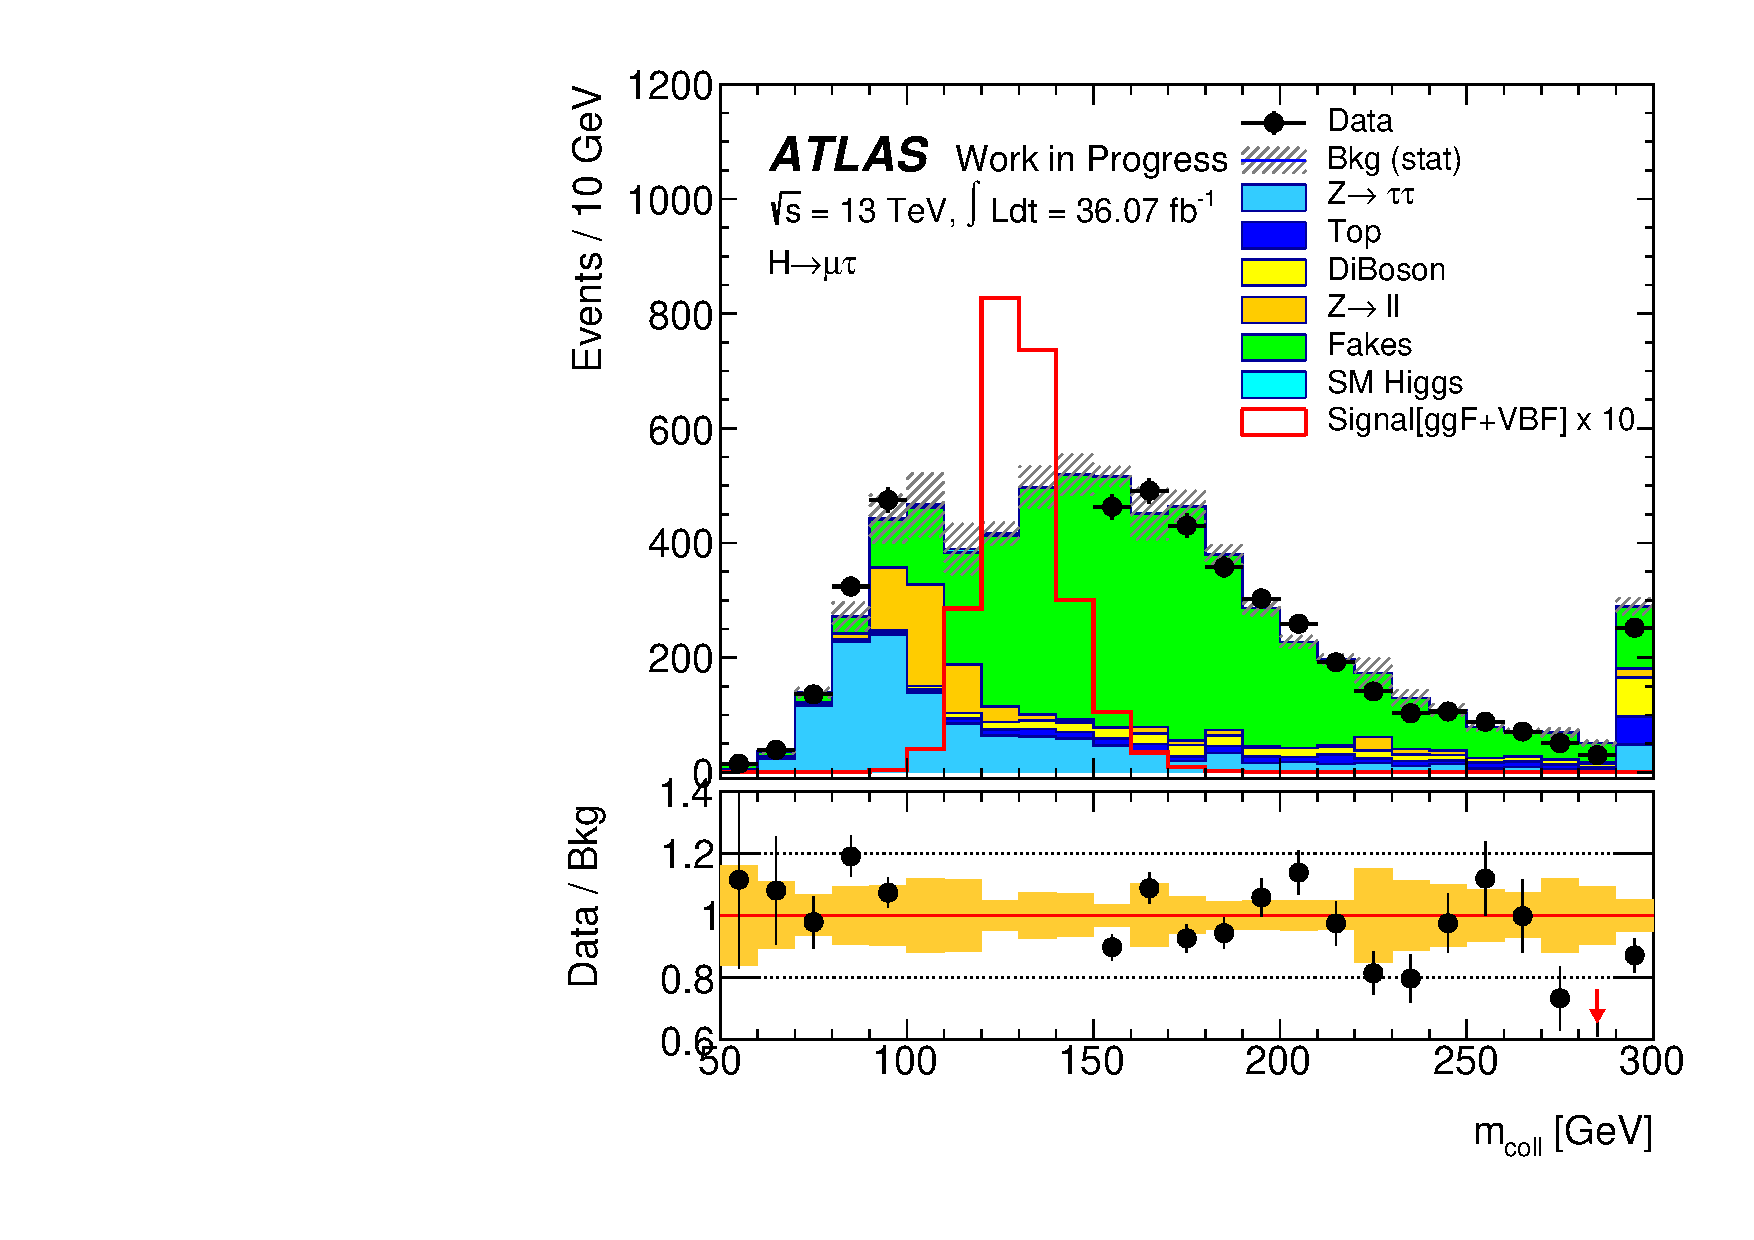
\includegraphics[width=.25\textwidth,height=.30\textheight,type=pdf,ext=.pdf,read=.pdf]{/afs/cern.ch/user/a/atpathak/afswork/public/Pixel/LFV_Plots/Plots_Qframework_25Apr2018_Final_note/plots_mcZll/mtau-CutTauMTSR1-collMassBL-lin}
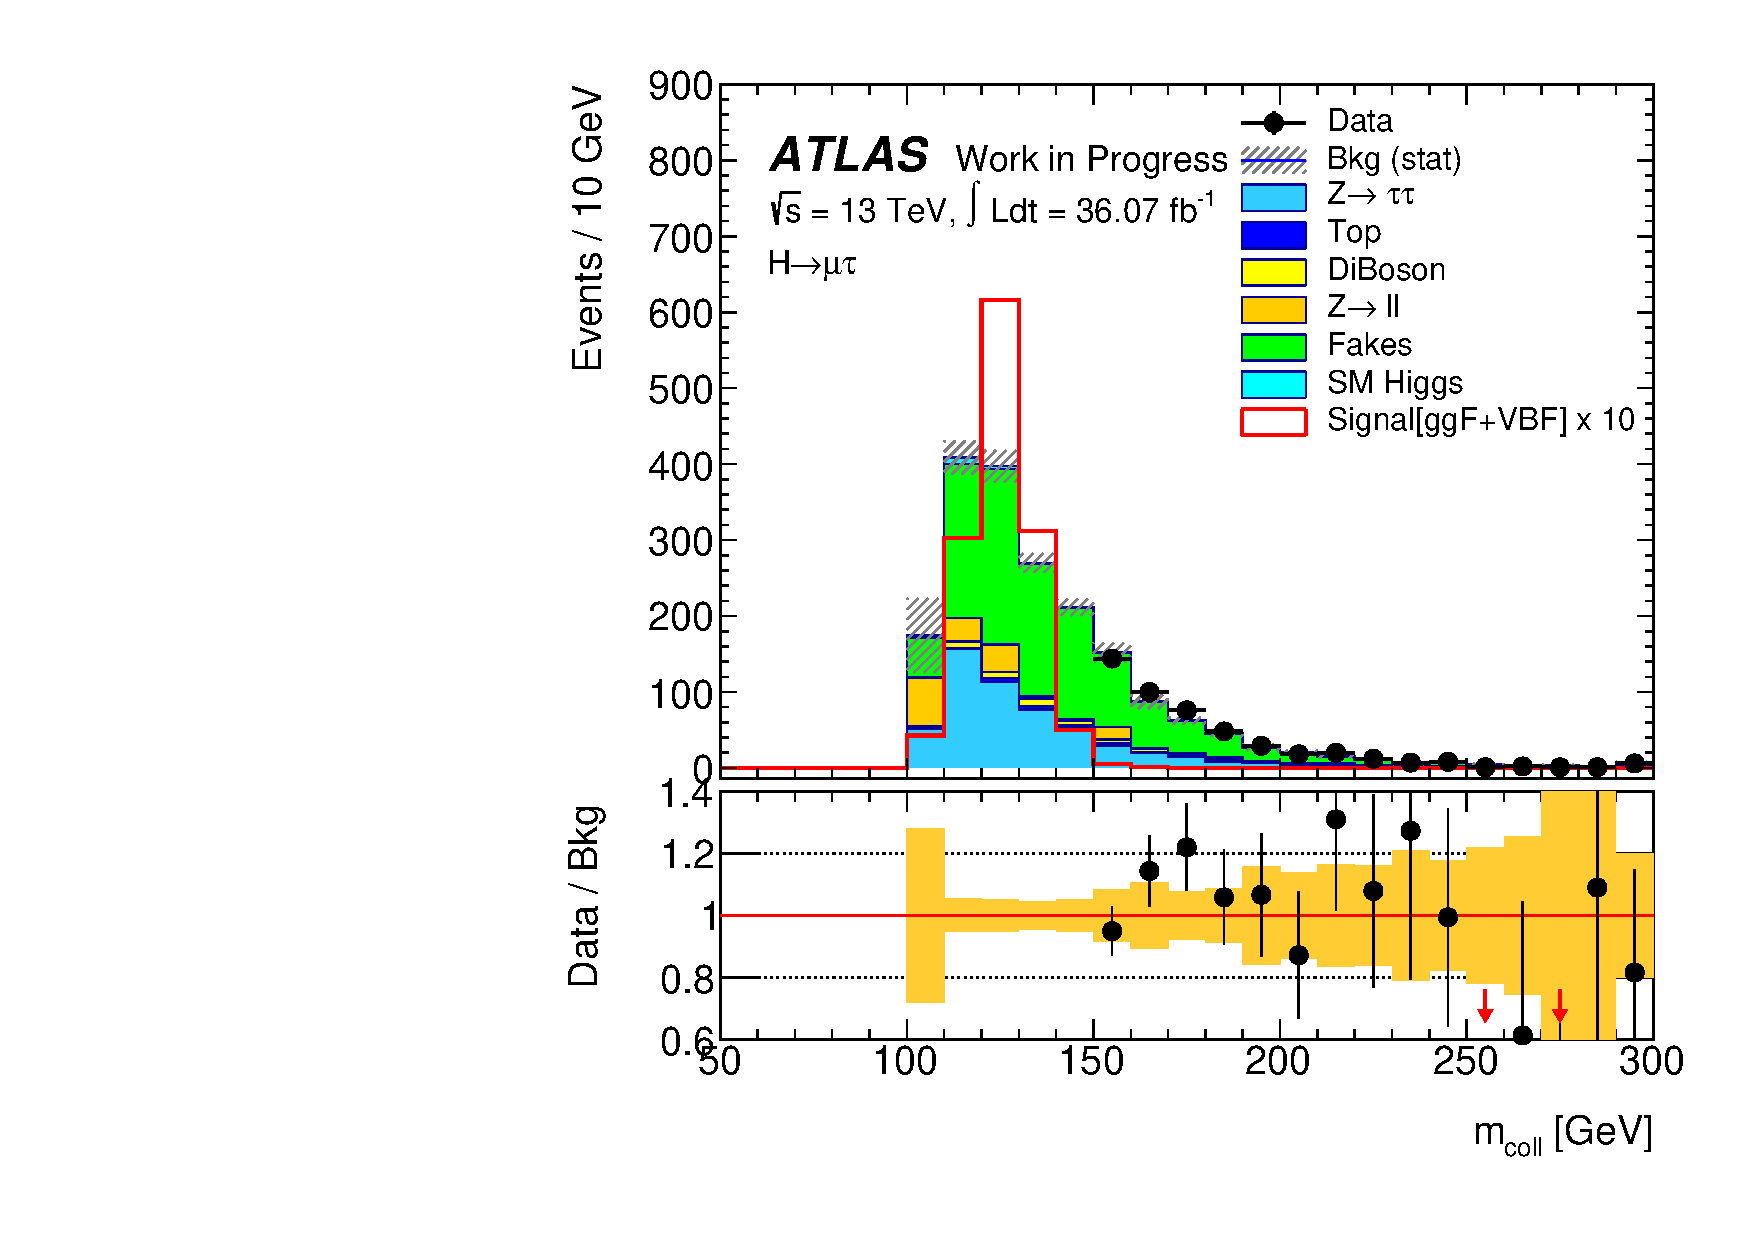
\includegraphics[width=.25\textwidth,height=.30\textheight,type=pdf,ext=.pdf,read=.pdf]{/afs/cern.ch/user/a/atpathak/afswork/public/Pixel/LFV_Plots/Plots_Qframework_25Apr2018_Final_note/plots_mcZll/mtau-CutTauMTSR2_Mvis-collMassBL-lin}
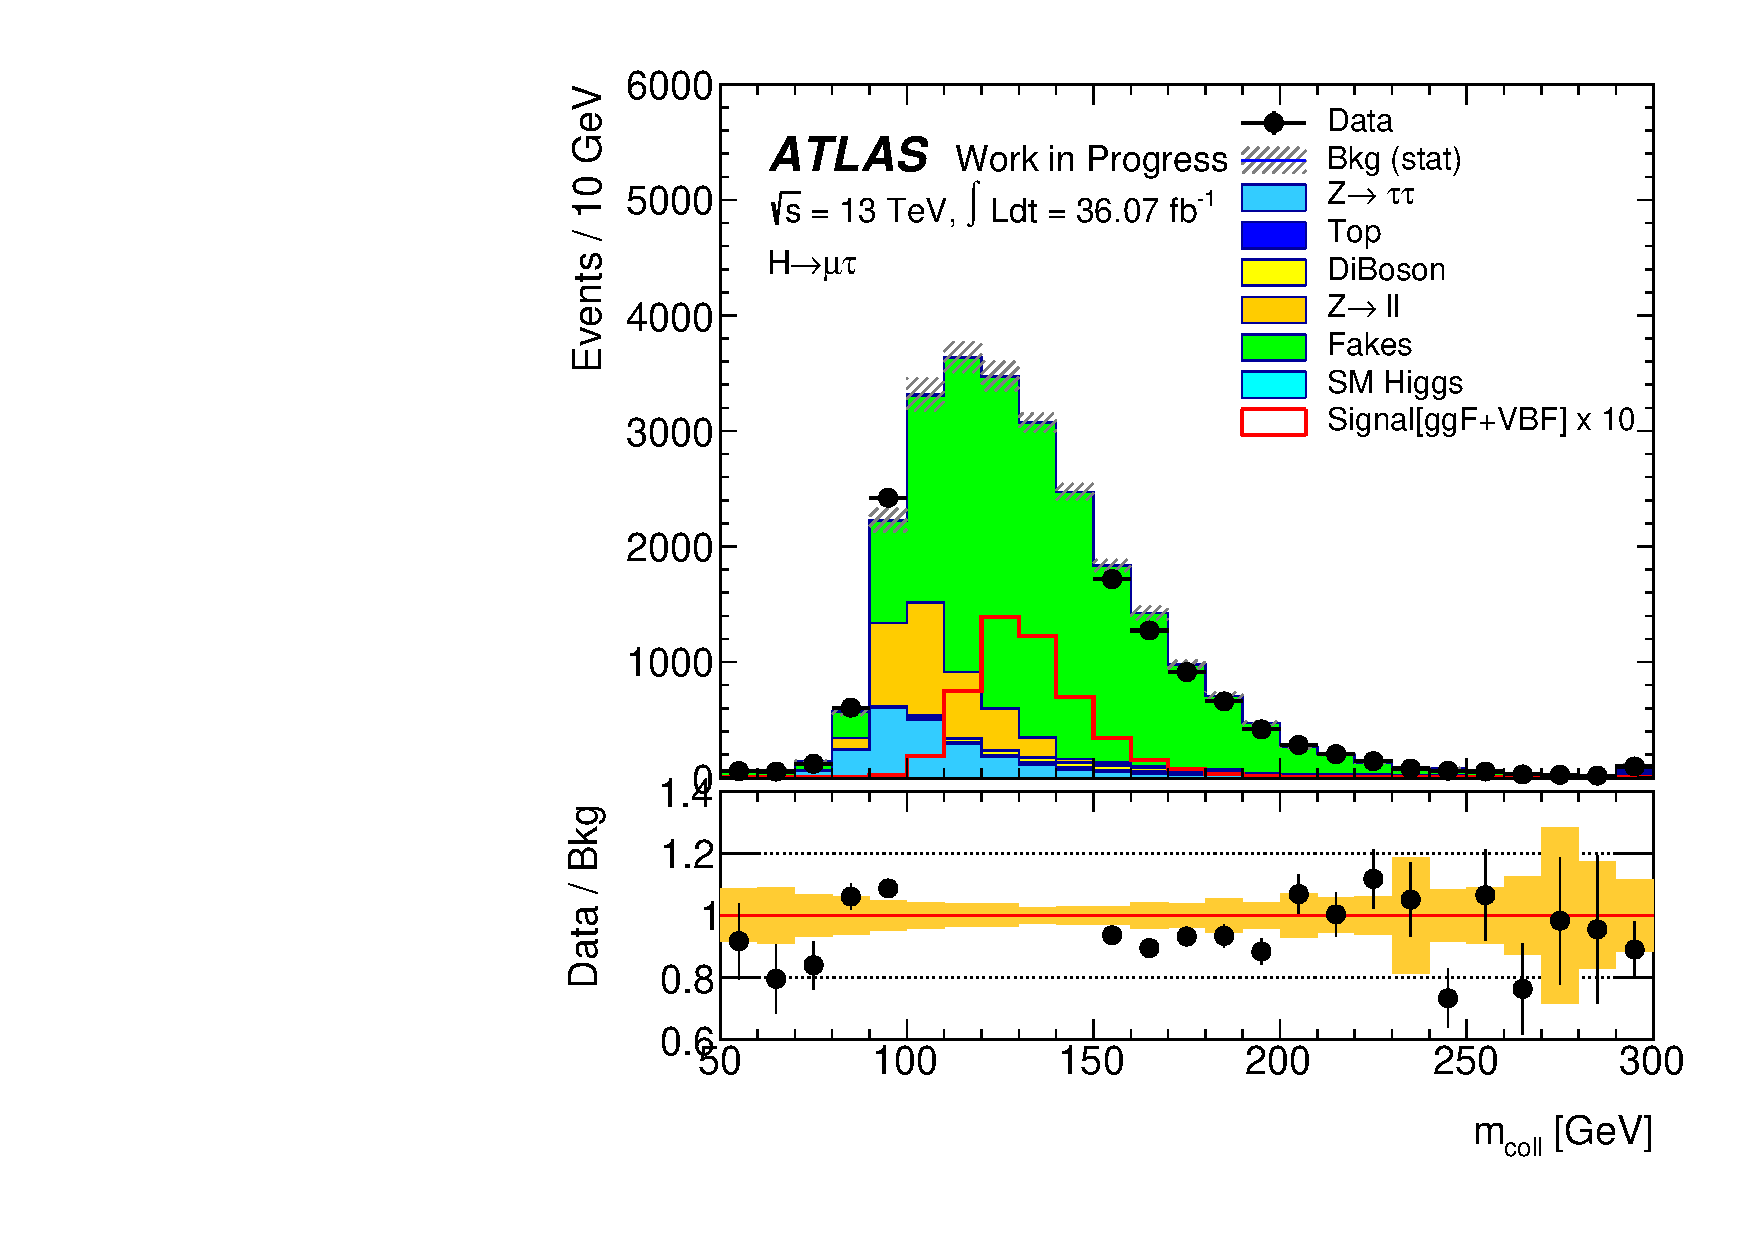
\includegraphics[width=.25\textwidth,height=.30\textheight,type=pdf,ext=.pdf,read=.pdf]{/afs/cern.ch/user/a/atpathak/afswork/public/Pixel/LFV_Plots/Plots_Qframework_25Apr2018_Final_note/plots_mcZll/mtau-CutTauPtSR3-collMassBL-lin}
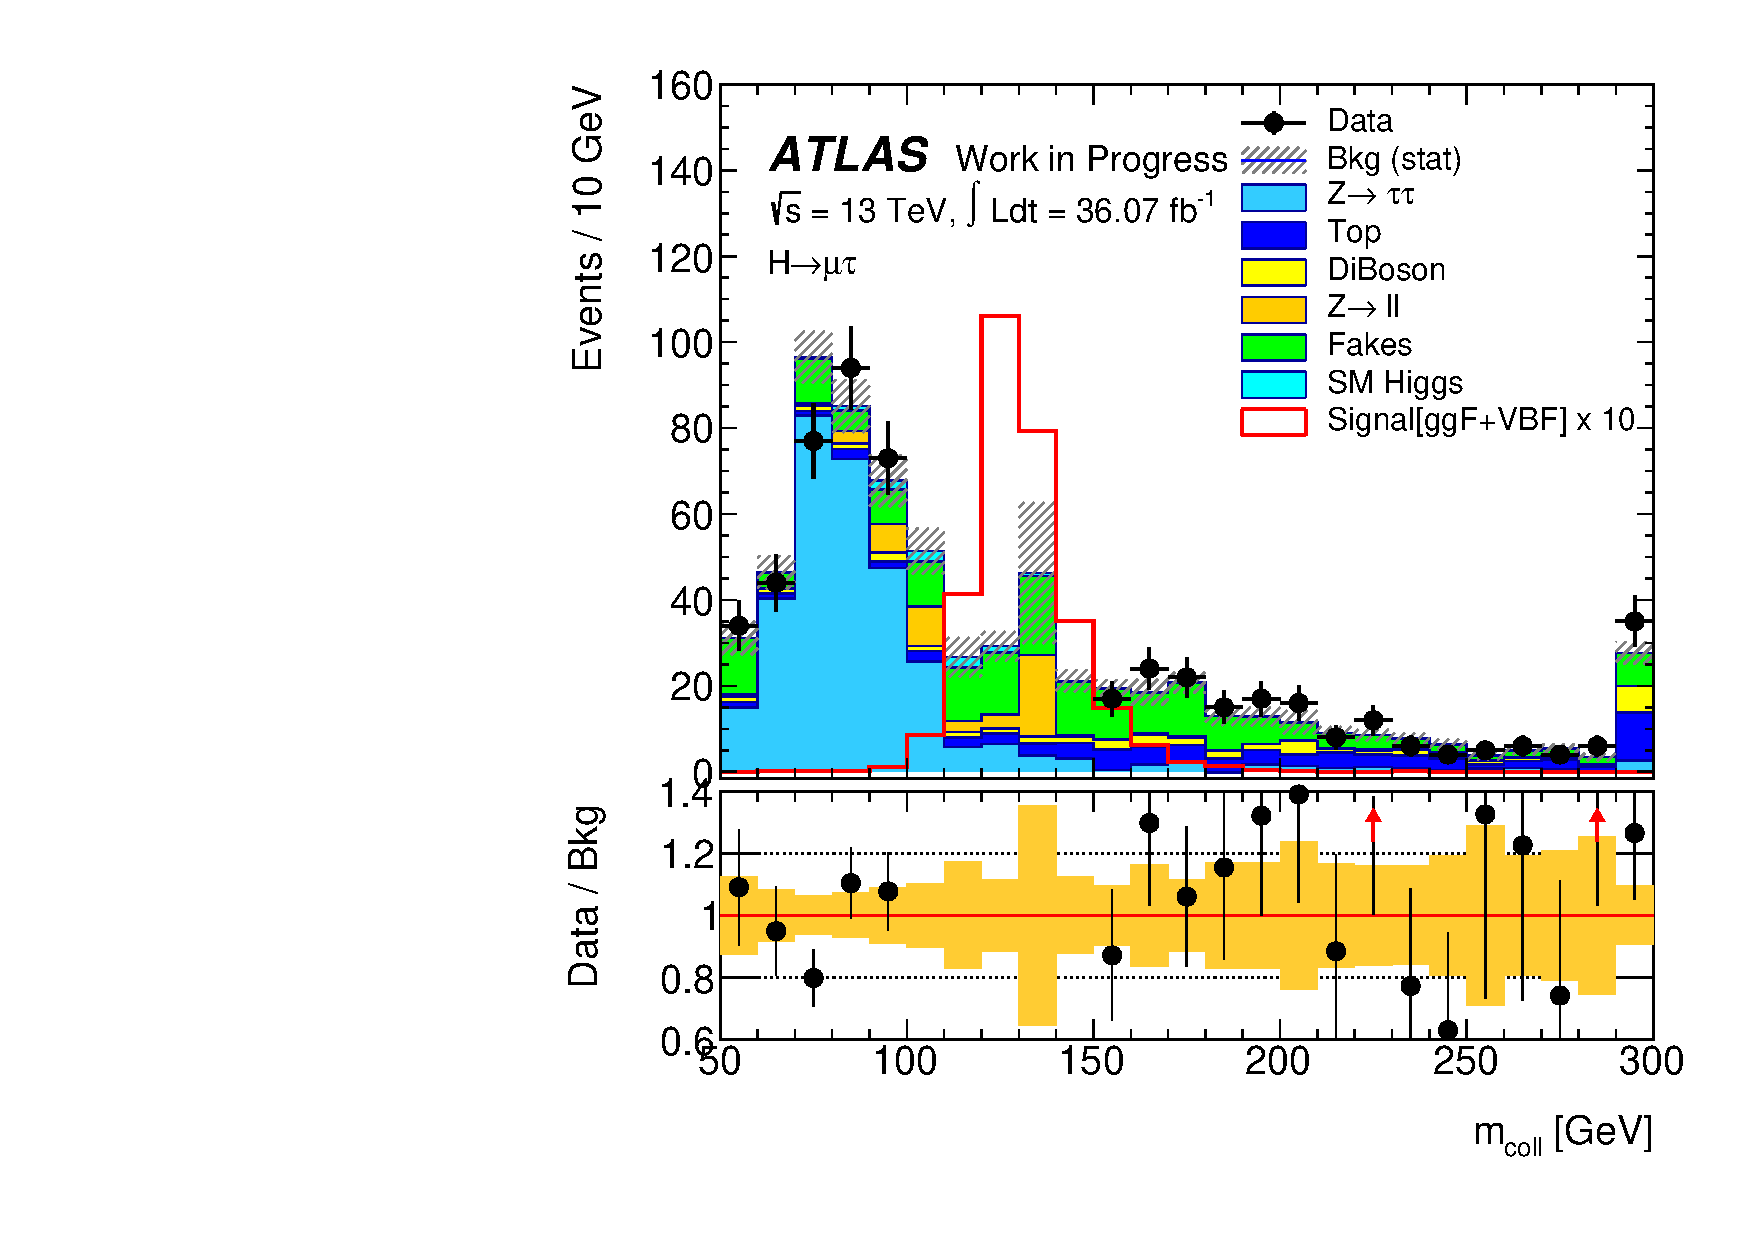
\includegraphics[width=.25\textwidth,height=.30\textheight,type=pdf,ext=.pdf,read=.pdf]{/afs/cern.ch/user/a/atpathak/afswork/public/Pixel/LFV_Plots/Plots_Qframework_25Apr2018_Final_note/plots_mcZll/mtau-CutVBF-collMassBL-lin}\\
\hspace{0.5in}SR1 
\hspace{0.75in}SR2
\hspace{0.75in}SR3
\hspace{0.75in}VBF
\end{normalsize}
\end{frame}
%-----------------------------------------------
\begin{frame}
\frametitle{SR plots for $e\tau_{had}$}
\begin{normalsize}
\vspace*{0.2cm}
\includegraphics[width=1.01\textwidth,height=.30\textheight,type=png,ext=.png,read=.png]{/afs/cern.ch/user/a/atpathak/afswork/public/Pixel/LFV_Plots/Plots_Qframework_25Apr2018_Final_note/Slides_comp/etau}\\
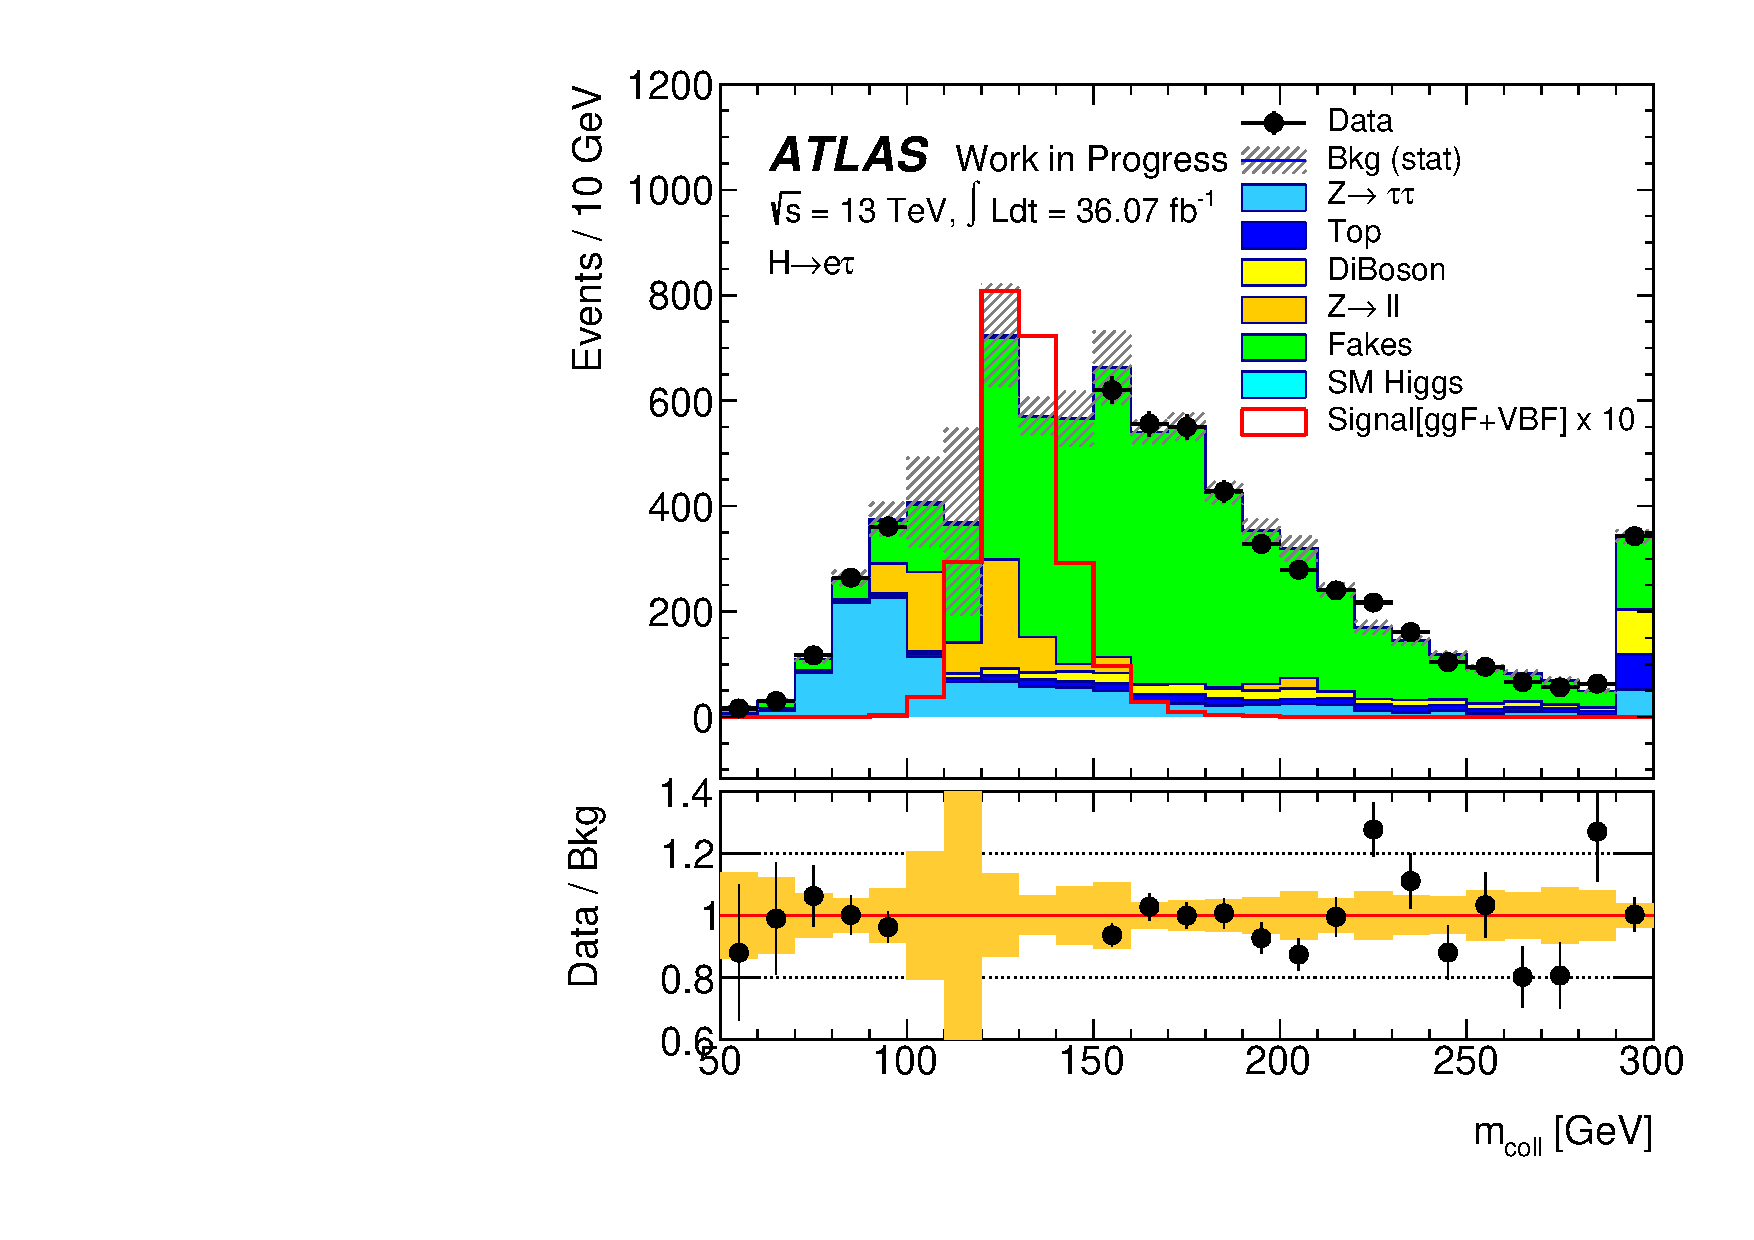
\includegraphics[width=.25\textwidth,height=.30\textheight,type=pdf,ext=.pdf,read=.pdf]{/afs/cern.ch/user/a/atpathak/afswork/public/Pixel/LFV_Plots/Plots_Qframework_25Apr2018_Final_note/plots_ddZll/etau-CutTauMTSR1-collMassBL-lin}
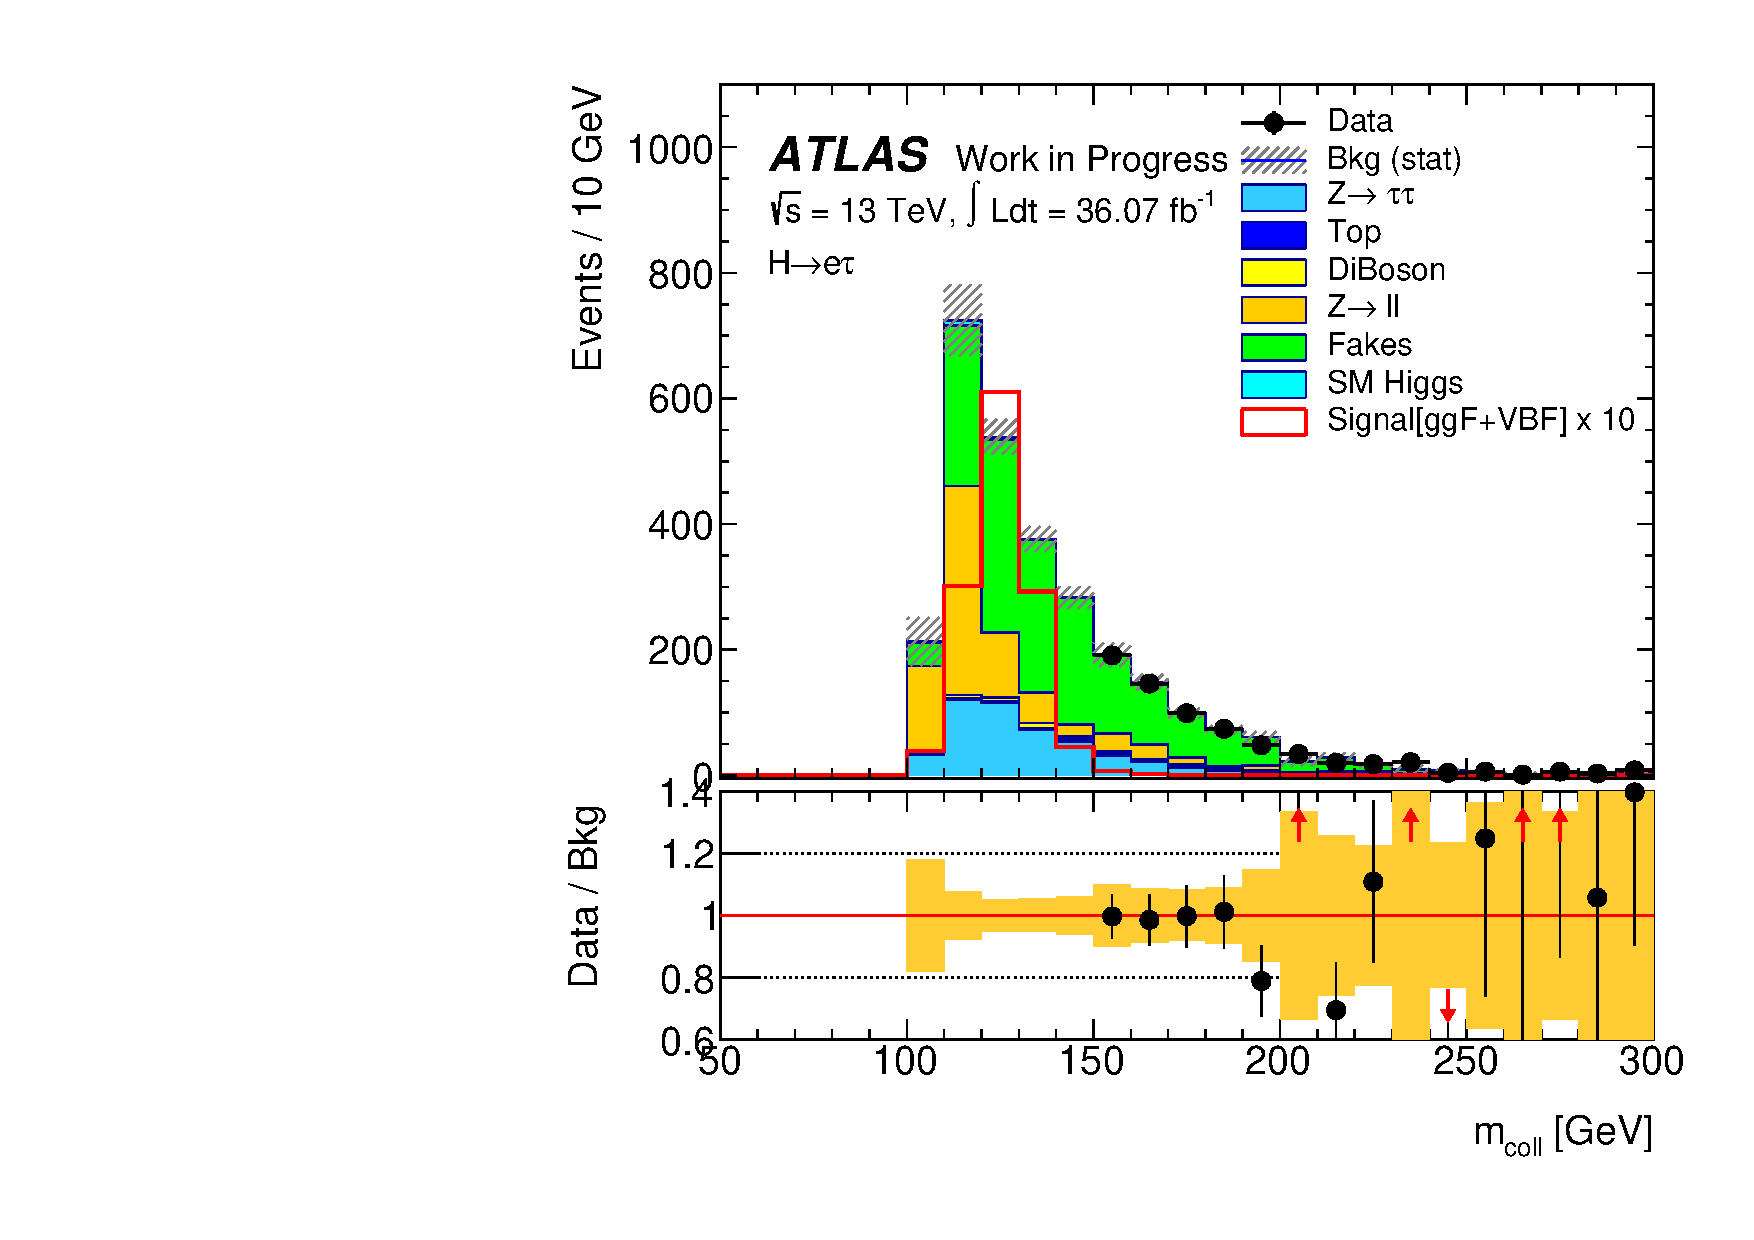
\includegraphics[width=.25\textwidth,height=.30\textheight,type=pdf,ext=.pdf,read=.pdf]{/afs/cern.ch/user/a/atpathak/afswork/public/Pixel/LFV_Plots/Plots_Qframework_25Apr2018_Final_note/plots_ddZll/etau-CutTauMTSR2_Mvis-collMassBL-lin}
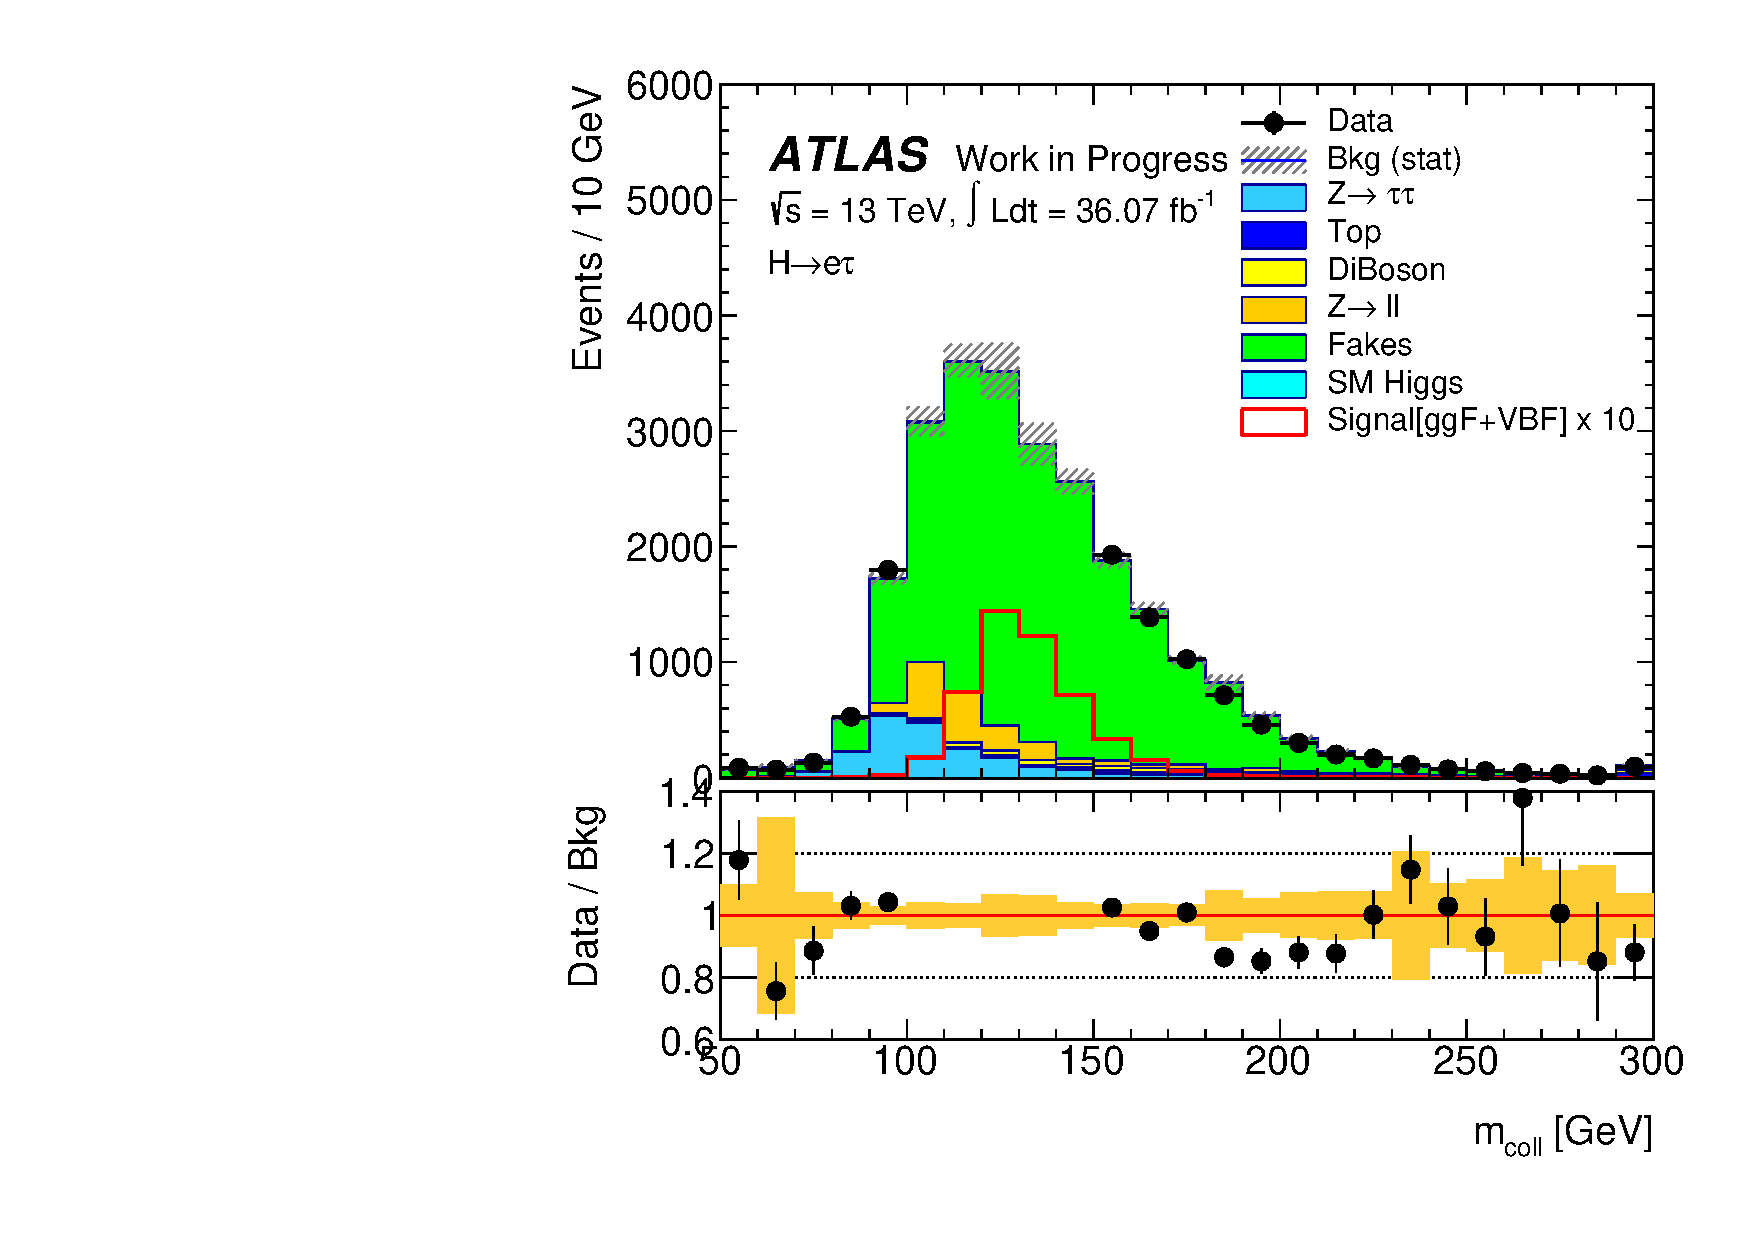
\includegraphics[width=.25\textwidth,height=.30\textheight,type=pdf,ext=.pdf,read=.pdf]{/afs/cern.ch/user/a/atpathak/afswork/public/Pixel/LFV_Plots/Plots_Qframework_25Apr2018_Final_note/plots_ddZll/etau-CutTauPtSR3-collMassBL-lin}
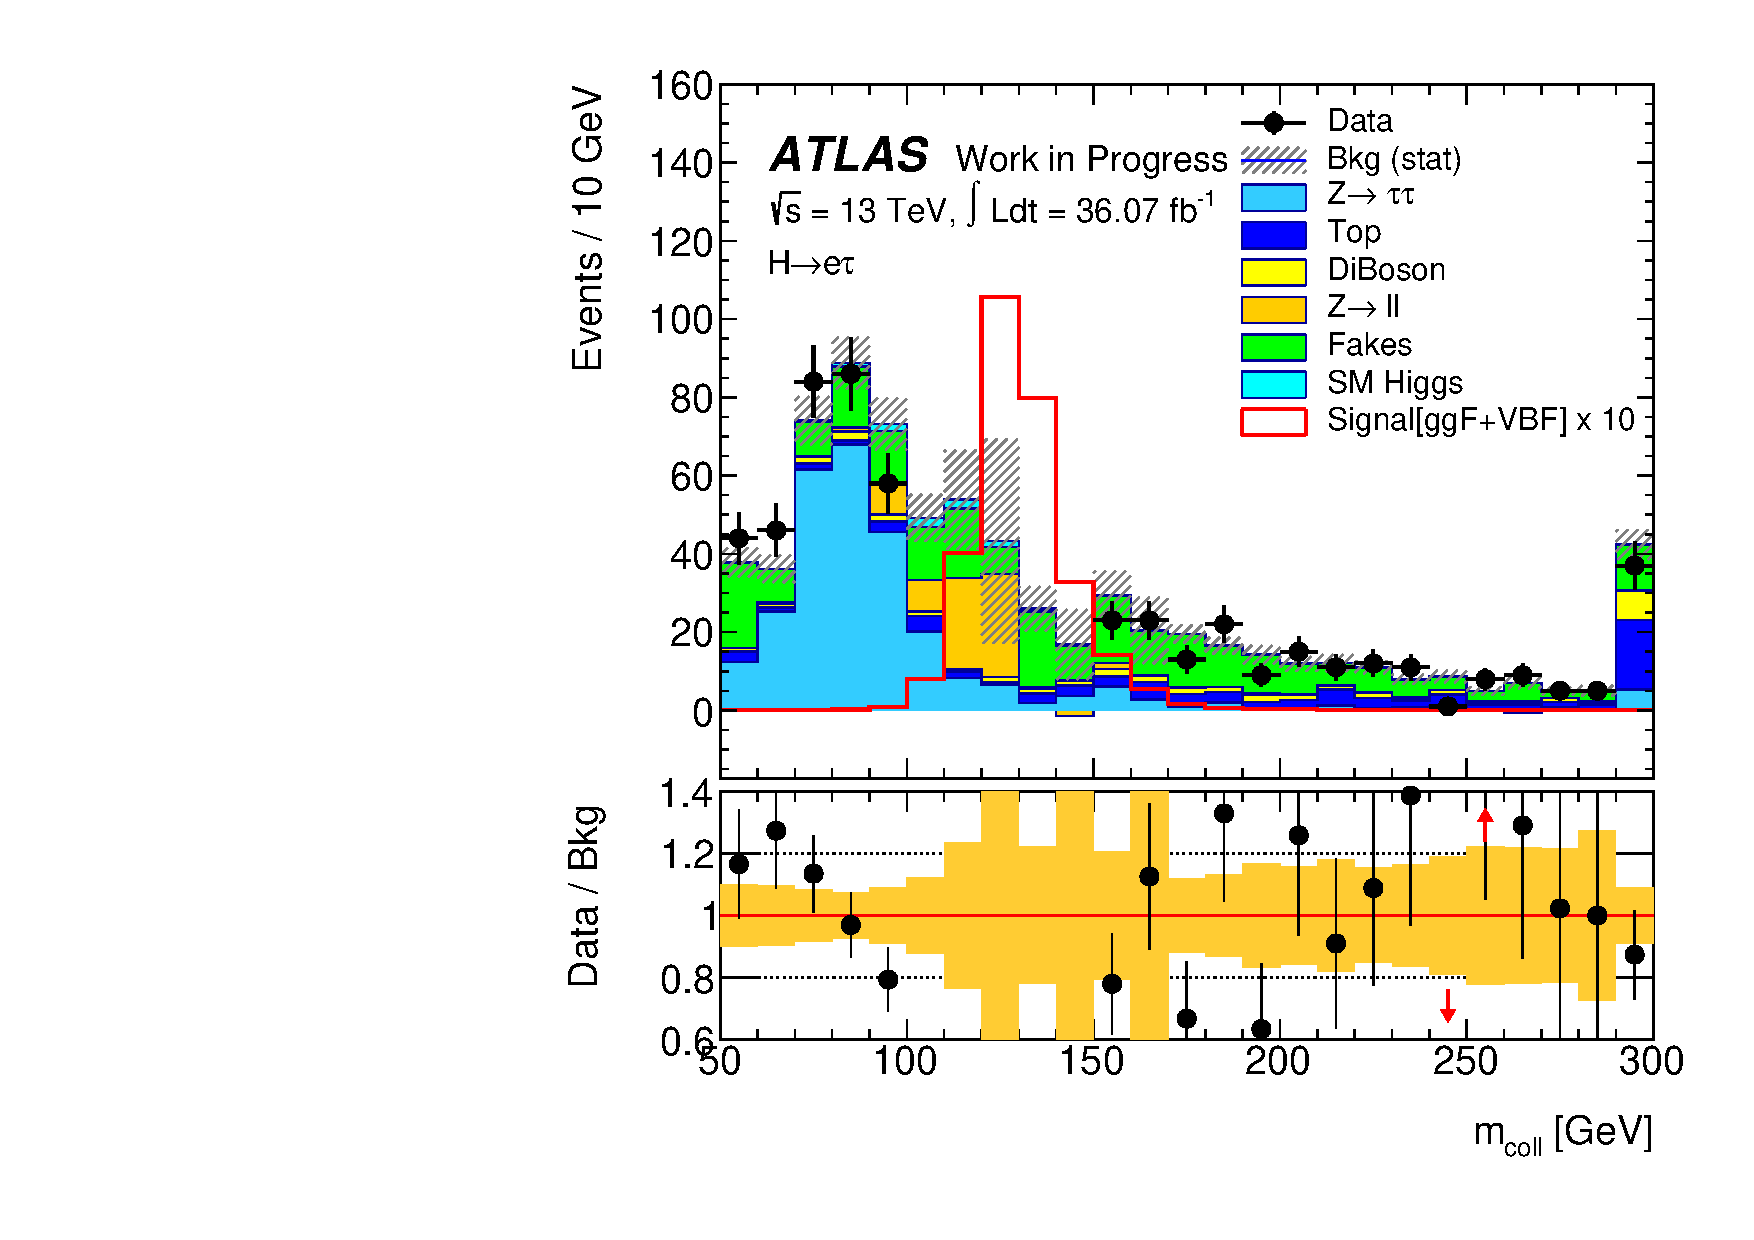
\includegraphics[width=.25\textwidth,height=.30\textheight,type=pdf,ext=.pdf,read=.pdf]{/afs/cern.ch/user/a/atpathak/afswork/public/Pixel/LFV_Plots/Plots_Qframework_25Apr2018_Final_note/plots_ddZll/etau-CutVBF-collMassBL-lin}\\
\hspace{0.5in}SR1 
\hspace{0.75in}SR2
\hspace{0.75in}SR3
\hspace{0.75in}VBF
\end{normalsize}
\end{frame}
%------------------------------------------------
\begin{frame}
\frametitle{H $\to \mu\tau $ }
\vspace{-5em}
\begin{center}
\begin{table}
{\scalebox{.29}{
\begin{tabular}{ c | c c |c  c  c  c  c  c  c | c c }
\ensuremath ${ \sqrt{s} }$=13 TeV  ,  \ensuremath $ {\int L}$ =36.07 fb${^{-1}} $ , \boldmath \ensuremath $ {\mu\tau} $ & ggF & VBF & Top & Z$\rightarrow \tau\tau$ & Z$\rightarrow$ ll & DiBoson & Fakes & SM Higgs & Total Bkg. & Data & Data/Bkg   \\
& & & & & & & & & & &  \\
\hline
Cut Base & \ensuremath{3242.35\pm 5.88} & \ensuremath{284.34\pm 0.68} & \ensuremath{1855234.20\pm 898.97} & \ensuremath{912252.15\pm 1259.58} &  & \ensuremath{184976.68\pm 233.39} & \ensuremath{35694063.96\pm 64352.28} & \ensuremath{3243.06\pm 5.86} & \ensuremath{44035582.91\pm 65745.74} & \ensuremath{42173465} & \ensuremath{0.96\pm 0.00}\tabularnewline
Cut Channel & \ensuremath{3176.68\pm 5.83} & \ensuremath{271.34\pm 0.66} & \ensuremath{863544.05\pm 598.92} & \ensuremath{581470.53\pm 1044.53} &  & \ensuremath{81196.63\pm 159.97} & \ensuremath{15936376.75\pm 49840.62} & \ensuremath{1787.82\pm 4.39} & \ensuremath{18372896.18\pm 50475.60} & \ensuremath{17507692} & \ensuremath{0.95\pm 0.00}\tabularnewline
Cut Hadronic Tau & \ensuremath{3045.89\pm 5.72} & \ensuremath{242.04\pm 0.63} & \ensuremath{863544.05\pm 598.92} & \ensuremath{581470.53\pm 1044.53} &  & \ensuremath{81196.63\pm 159.97} & \ensuremath{15936376.75\pm 49840.62} & \ensuremath{1787.82\pm 4.39} & \ensuremath{18372896.18\pm 50475.60} & \ensuremath{17507692} & \ensuremath{0.95\pm 0.00}\tabularnewline
Cut Trigger & \ensuremath{2936.65\pm 5.62} & \ensuremath{225.40\pm 0.60} & \ensuremath{747576.16\pm 552.11} & \ensuremath{327835.61\pm 705.96} &  & \ensuremath{70845.83\pm 150.18} & \ensuremath{16042731.90\pm 46447.02} & \ensuremath{1303.46\pm 3.70} & \ensuremath{17899700.89\pm 47050.45} & \ensuremath{17150842} & \ensuremath{0.96\pm 0.00}\tabularnewline
Cut NPVX & \ensuremath{2754.84\pm 5.44} & \ensuremath{210.23\pm 0.58} & \ensuremath{702946.97\pm 535.30} & \ensuremath{304382.92\pm 683.26} &  & \ensuremath{66433.97\pm 144.93} & \ensuremath{15921151.31\pm 44433.15} & \ensuremath{1221.40\pm 3.59} & \ensuremath{17656278.13\pm 45050.72} & \ensuremath{16952130} & \ensuremath{0.96\pm 0.00}\tabularnewline
Cut LepQual & \ensuremath{2632.40\pm 5.31} & \ensuremath{202.58\pm 0.57} & \ensuremath{669385.63\pm 520.36} & \ensuremath{288629.62\pm 663.20} &  & \ensuremath{63820.19\pm 141.63} & \ensuremath{13002424.18\pm 43551.75} & \ensuremath{1156.31\pm 3.48} & \ensuremath{14649329.82\pm 44171.24} & \ensuremath{13978796} & \ensuremath{0.95\pm 0.00}\tabularnewline
Cut TauQual & \ensuremath{2594.85\pm 5.27} & \ensuremath{199.94\pm 0.57} & \ensuremath{654007.63\pm 514.27} & \ensuremath{282537.44\pm 657.06} &  & \ensuremath{61880.63\pm 139.46} & \ensuremath{12558776.00\pm 43142.75} & \ensuremath{1138.35\pm 3.45} & \ensuremath{14159701.69\pm 43760.28} & \ensuremath{13504580} & \ensuremath{0.95\pm 0.00}\tabularnewline
Cut OS & \ensuremath{2551.38\pm 5.22} & \ensuremath{196.60\pm 0.56} & \ensuremath{428556.67\pm 416.35} & \ensuremath{265900.61\pm 612.56} &  & \ensuremath{42222.52\pm 116.68} & \ensuremath{7691105.80\pm 28917.12} & \ensuremath{1051.13\pm 3.34} & \ensuremath{8752936.54\pm 29717.63} & \ensuremath{8323578} & \ensuremath{0.95\pm 0.00}\tabularnewline
Cut Tau/AntiTau & \ensuremath{1529.13\pm 4.05} & \ensuremath{119.11\pm 0.44} & \ensuremath{45217.91\pm 138.82} & \ensuremath{144218.69\pm 426.94} &  & \ensuremath{6607.64\pm 38.02} & \ensuremath{511317.69\pm 10679.70} & \ensuremath{603.74\pm 2.55} & \ensuremath{743301.55\pm 10723.16} & \ensuremath{564526} & \ensuremath{0.76\pm 0.01}\tabularnewline
LepPt > 27 GeV & \ensuremath{1524.42\pm 4.04} & \ensuremath{118.49\pm 0.44} & \ensuremath{36244.61\pm 124.93} & \ensuremath{132343.49\pm 398.71} &  & \ensuremath{5645.66\pm 32.97} & \ensuremath{1391641.35\pm 2189.99} & \ensuremath{580.76\pm 2.50} & \ensuremath{1593232.06\pm 2336.53} & \ensuremath{475228} & \ensuremath{0.30\pm 0.00}\tabularnewline
TauPt > 25 GeV & \ensuremath{1394.50\pm 3.86} & \ensuremath{110.05\pm 0.42} & \ensuremath{31841.23\pm 117.22} & \ensuremath{108750.96\pm 350.31} &  & \ensuremath{4841.41\pm 30.62} & \ensuremath{907907.36\pm 1559.10} & \ensuremath{532.96\pm 2.40} & \ensuremath{1077866.50\pm 1731.19} & \ensuremath{345220} & \ensuremath{0.32\pm 0.00}\tabularnewline
Cut Zee Veto & \ensuremath{1394.50\pm 3.86} & \ensuremath{110.05\pm 0.42} & \ensuremath{31841.23\pm 117.22} & \ensuremath{108750.96\pm 350.31} &  & \ensuremath{4841.41\pm 30.62} & \ensuremath{907907.36\pm 1559.10} & \ensuremath{532.96\pm 2.40} & \ensuremath{1077866.50\pm 1731.19} & \ensuremath{345220} & \ensuremath{0.32\pm 0.00}\tabularnewline
$\sum cos(\Delta\phi) > -0.35$ & \ensuremath{1228.08\pm 3.65} & \ensuremath{91.73\pm 0.38} & \ensuremath{22703.20\pm 99.63} & \ensuremath{101947.30\pm 335.17} &  & \ensuremath{2965.25\pm 23.39} & \ensuremath{87814.98\pm 360.01} & \ensuremath{487.17\pm 2.29} & \ensuremath{237349.18\pm 788.44} & \ensuremath{240252} & \ensuremath{1.01\pm 0.00}\tabularnewline
$\Delta\eta(l,\tau) < 2$ & \ensuremath{1188.17\pm 3.58} & \ensuremath{89.82\pm 0.38} & \ensuremath{19745.61\pm 93.01} & \ensuremath{101544.90\pm 334.20} &  & \ensuremath{2549.48\pm 21.50} & \ensuremath{70572.88\pm 334.17} & \ensuremath{482.53\pm 2.28} & \ensuremath{215918.69\pm 771.38} & \ensuremath{218957} & \ensuremath{1.01\pm 0.00}\tabularnewline
Nbjet = 0 & \ensuremath{1113.37\pm 3.43} & \ensuremath{78.64\pm 0.34} & \ensuremath{1817.55\pm 25.94} & \ensuremath{95464.88\pm 314.59} &  & \ensuremath{2247.58\pm 20.10} & \ensuremath{59417.73\pm 320.30} & \ensuremath{438.64\pm 2.16} & \ensuremath{179283.54\pm 740.07} & \ensuremath{185091} & \ensuremath{1.03\pm 0.00}\tabularnewline
Preselection & \ensuremath{1113.37\pm 3.43} & \ensuremath{78.64\pm 0.34} & \ensuremath{1817.55\pm 25.94} & \ensuremath{95464.88\pm 314.59} &  & \ensuremath{2247.58\pm 20.10} & \ensuremath{65237.46\pm 343.23} & \ensuremath{438.64\pm 2.16} & \ensuremath{185103.27\pm 750.28} & \ensuremath{185091} & \ensuremath{1.00\pm 0.00}\tabularnewline
\hline
TauPt > 45 GeV & \ensuremath{453.32\pm 2.15} & \ensuremath{42.85\pm 0.25} & \ensuremath{895.17\pm 18.41} & \ensuremath{12027.74\pm 113.19} &  & \ensuremath{1046.20\pm 13.67} & \ensuremath{13570.67\pm 128.44} & \ensuremath{180.27\pm 1.35} & \ensuremath{30818.58\pm 296.31} & \ensuremath{30554} & \ensuremath{0.99\pm 0.01}\tabularnewline
SR1: $m_{T}(l,MET) > 40$ GeV & \ensuremath{282.54\pm 1.68} & \ensuremath{29.07\pm 0.21} & \ensuremath{684.74\pm 16.14} & \ensuremath{1984.39\pm 50.24} &  & \ensuremath{760.22\pm 11.78} & \ensuremath{8747.56\pm 97.18} & \ensuremath{35.63\pm 0.60} & \ensuremath{12982.06\pm 156.53} & \ensuremath{12338} & \ensuremath{0.95\pm 0.01}\tabularnewline
SR1: $m_{T}(\tau,MET) < 30$ GeV & \ensuremath{211.56\pm 1.44} & \ensuremath{23.19\pm 0.19} & \ensuremath{246.51\pm 9.21} & \ensuremath{1317.07\pm 39.20} &  & \ensuremath{329.78\pm 7.75} & \ensuremath{4250.47\pm 81.49} & \ensuremath{21.68\pm 0.45} & \ensuremath{6686.33\pm 126.69} & \ensuremath{6703} & \ensuremath{1.00\pm 0.02}\tabularnewline
\hline
TauPt > 45 GeV & \ensuremath{453.32\pm 2.15} & \ensuremath{42.85\pm 0.25} & \ensuremath{895.17\pm 18.41} & \ensuremath{12027.74\pm 113.19} &  & \ensuremath{1046.20\pm 13.67} & \ensuremath{13570.67\pm 128.44} & \ensuremath{180.27\pm 1.35} & \ensuremath{30818.58\pm 296.31} & \ensuremath{30554} & \ensuremath{0.99\pm 0.01}\tabularnewline
SR2: $m_{T}(l,MET) < 40$ GeV & \ensuremath{170.78\pm 1.34} & \ensuremath{13.78\pm 0.14} & \ensuremath{210.43\pm 8.85} & \ensuremath{10043.35\pm 101.43} &  & \ensuremath{285.98\pm 6.94} & \ensuremath{4823.11\pm 83.98} & \ensuremath{144.64\pm 1.21} & \ensuremath{17836.52\pm 251.59} & \ensuremath{18216} & \ensuremath{1.02\pm 0.02}\tabularnewline
SR2: $m_{T}(\tau,MET) < 60$ GeV & \ensuremath{133.33\pm 1.19} & \ensuremath{11.20\pm 0.13} & \ensuremath{64.82\pm 4.56} & \ensuremath{6346.12\pm 77.72} &  & \ensuremath{133.40\pm 4.57} & \ensuremath{2136.19\pm 71.49} & \ensuremath{74.59\pm 0.85} & \ensuremath{10629.44\pm 222.69} & \ensuremath{10975} & \ensuremath{1.03\pm 0.02}\tabularnewline
SR2: lephad\_vis\_mass > 100 GeV & \ensuremath{123.77\pm 1.16} & \ensuremath{9.25\pm 0.12} & \ensuremath{25.07\pm 2.88} & \ensuremath{548.48\pm 18.37} &  & \ensuremath{58.55\pm 3.58} & \ensuremath{1118.91\pm 24.54} & \ensuremath{16.60\pm 0.41} & \ensuremath{1916.33\pm 62.62} & \ensuremath{1906} & \ensuremath{0.99\pm 0.04}\tabularnewline
\hline
SR3: LepPt > 45 GeV & \ensuremath{919.76\pm 3.14} & \ensuremath{58.29\pm 0.30} & \ensuremath{1301.05\pm 22.31} & \ensuremath{9181.74\pm 80.05} &  & \ensuremath{1561.56\pm 16.96} & \ensuremath{30668.10\pm 241.93} & \ensuremath{128.92\pm 1.12} & \ensuremath{48913.88\pm 409.83} & \ensuremath{54935} & \ensuremath{1.12\pm 0.01}\tabularnewline
SR3: TauPt < 45 GeV & \ensuremath{467.06\pm 2.27} & \ensuremath{21.44\pm 0.18} & \ensuremath{272.08\pm 9.75} & \ensuremath{2231.60\pm 37.66} &  & \ensuremath{440.19\pm 9.41} & \ensuremath{19450.19\pm 199.91} & \ensuremath{32.00\pm 0.62} & \ensuremath{25440.37\pm 300.52} & \ensuremath{25481} & \ensuremath{1.00\pm 0.01}\tabularnewline
\hline
VBF SR & \ensuremath{10.07\pm 0.28} & \ensuremath{19.67\pm 0.17} & \ensuremath{72.71\pm 4.91} & \ensuremath{317.94\pm 13.01} &  & \ensuremath{40.50\pm 3.24} & \ensuremath{186.22\pm 7.73} & \ensuremath{10.81\pm 0.20} & \ensuremath{674.56\pm 23.13} & \ensuremath{699} & \ensuremath{1.04\pm 0.05}
\end{tabular}
}}
\end{table}
\end{center}
\end{frame}
%-----------------------------------------------
\begin{frame}
\frametitle{H $\to e\tau $ }
\vspace{-5em}
\begin{center}
\begin{table}
{\scalebox{.27}{
\begin{tabular}{ c | c c |c  c  c  c  c  c  c | c c }
%\ensuremath{\sqrt{s}=13 TeV}, \ensuremath{\mathcal{L}=36.07 fb^{-1}}, \textbf{\ensuremath{e\tau}} & ggF & VBF & Top & Z\rightarrow \tau\tau & Z\rightarrow ll & DiBoson & Fakes & SM Higgs & Total Bkg. & Data & Data/Bkg\tabularnewline
\ensuremath ${ \sqrt{s} }$=13 TeV  ,  \ensuremath $ {\int L}$ =36.07 fb${^{-1}} $ , \boldmath \ensuremath $ {e\tau} $ & ggF & VBF & Top & Z$\rightarrow \tau\tau$ & Z$\rightarrow$ ll & DiBoson & Fakes & SM Higgs & Total Bkg. & Data & Data/Bkg   \\
& & & & & & & & & & &  \\
\hline
Cut Base & \ensuremath{3511.17\pm 6.20} & \ensuremath{297.69\pm 0.70} & \ensuremath{1855234.20\pm 898.97} & \ensuremath{912252.15\pm 1259.58} & \ensuremath{-14908.00\pm 21103.05} & \ensuremath{184976.68\pm 233.39} & \ensuremath{35694063.96\pm 64352.28} & \ensuremath{3243.06\pm 5.86} & \ensuremath{44020674.91\pm 69049.56} & \ensuremath{42173465} & \ensuremath{0.96\pm 0.00}\tabularnewline
Cut Channel & \ensuremath{3455.00\pm 6.15} & \ensuremath{286.81\pm 0.69} & \ensuremath{899429.34\pm 639.55} & \ensuremath{316717.06\pm 695.04} & \ensuremath{-7623.00\pm 12984.40} & \ensuremath{81550.48\pm 161.09} & \ensuremath{19969497.10\pm 39932.20} & \ensuremath{1377.86\pm 3.80} & \ensuremath{23078780.13\pm 42728.07} & \ensuremath{22185032} & \ensuremath{0.96\pm 0.00}\tabularnewline
Cut Hadronic Tau & \ensuremath{3304.35\pm 6.02} & \ensuremath{254.57\pm 0.65} & \ensuremath{899429.34\pm 639.55} & \ensuremath{316717.06\pm 695.04} & \ensuremath{-7623.00\pm 12984.40} & \ensuremath{81550.48\pm 161.09} & \ensuremath{19969497.10\pm 39932.20} & \ensuremath{1377.86\pm 3.80} & \ensuremath{23078780.13\pm 42728.07} & \ensuremath{22185032} & \ensuremath{0.96\pm 0.00}\tabularnewline
Cut Trigger & \ensuremath{3102.87\pm 5.84} & \ensuremath{241.56\pm 0.63} & \ensuremath{823376.24\pm 605.74} & \ensuremath{278484.63\pm 644.75} & \ensuremath{-7391.00\pm 12378.67} & \ensuremath{75524.07\pm 155.28} & \ensuremath{19575227.67\pm 37862.51} & \ensuremath{1239.16\pm 3.59} & \ensuremath{22335333.01\pm 40524.78} & \ensuremath{21517570} & \ensuremath{0.96\pm 0.00}\tabularnewline
Cut NPVX & \ensuremath{2910.99\pm 5.65} & \ensuremath{225.69\pm 0.61} & \ensuremath{774938.44\pm 587.55} & \ensuremath{259229.24\pm 625.99} & \ensuremath{-7324.00\pm 12057.59} & \ensuremath{70857.61\pm 150.57} & \ensuremath{19496619.98\pm 36775.52} & \ensuremath{1162.45\pm 3.48} & \ensuremath{22074421.93\pm 39364.32} & \ensuremath{21305142} & \ensuremath{0.97\pm 0.00}\tabularnewline
Cut LepQual & \ensuremath{2804.53\pm 5.55} & \ensuremath{218.55\pm 0.60} & \ensuremath{734405.28\pm 569.20} & \ensuremath{246631.86\pm 613.47} & \ensuremath{-5786.00\pm 11418.61} & \ensuremath{68039.44\pm 147.58} & \ensuremath{14385781.27\pm 35977.04} & \ensuremath{1102.04\pm 3.38} & \ensuremath{16842343.38\pm 38394.38} & \ensuremath{16112129} & \ensuremath{0.96\pm 0.00}\tabularnewline
Cut TauQual & \ensuremath{2768.42\pm 5.51} & \ensuremath{216.03\pm 0.60} & \ensuremath{718152.71\pm 563.03} & \ensuremath{242494.40\pm 608.73} & \ensuremath{-5537.00\pm 11118.56} & \ensuremath{65879.97\pm 145.24} & \ensuremath{13864374.92\pm 35533.63} & \ensuremath{1087.40\pm 3.36} & \ensuremath{16193052.82\pm 37853.70} & \ensuremath{15478905} & \ensuremath{0.96\pm 0.00}\tabularnewline
Cut OS & \ensuremath{2705.78\pm 5.45} & \ensuremath{210.81\pm 0.59} & \ensuremath{468838.87\pm 454.04} & \ensuremath{227434.53\pm 579.92} & \ensuremath{-3228.00\pm 9381.51} & \ensuremath{44844.61\pm 120.78} & \ensuremath{8023471.80\pm 29426.03} & \ensuremath{996.56\pm 3.23} & \ensuremath{9639706.60\pm 31447.40} & \ensuremath{9173022} & \ensuremath{0.95\pm 0.00}\tabularnewline
Cut Tau/AntiTau & \ensuremath{1612.30\pm 4.21} & \ensuremath{126.80\pm 0.46} & \ensuremath{49572.98\pm 153.03} & \ensuremath{122701.57\pm 378.27} & \ensuremath{-1350323.33\pm 4818.42} & \ensuremath{7333.47\pm 44.70} & \ensuremath{605104.44\pm 10726.92} & \ensuremath{571.20\pm 2.46} & \ensuremath{-328165.51\pm 12169.48} & \ensuremath{620478} & \ensuremath{-1.89\pm -0.07}\tabularnewline
LepPt > 27 GeV & \ensuremath{1609.56\pm 4.21} & \ensuremath{126.44\pm 0.46} & \ensuremath{40261.45\pm 139.83} & \ensuremath{116807.89\pm 366.98} & \ensuremath{-1352150.63\pm 4592.01} & \ensuremath{6375.10\pm 40.93} & \ensuremath{1559177.11\pm 3962.93} & \ensuremath{557.96\pm 2.44} & \ensuremath{596152.60\pm 6805.30} & \ensuremath{589725} & \ensuremath{0.99\pm 0.01}\tabularnewline
TauPt > 25 GeV & \ensuremath{1477.57\pm 4.03} & \ensuremath{117.08\pm 0.44} & \ensuremath{35547.51\pm 131.56} & \ensuremath{95974.73\pm 332.71} & \ensuremath{-898731.02\pm 4185.34} & \ensuremath{5527.50\pm 38.45} & \ensuremath{1007523.17\pm 3384.33} & \ensuremath{510.83\pm 2.33} & \ensuremath{460520.17\pm 6157.22} & \ensuremath{448166} & \ensuremath{0.97\pm 0.01}\tabularnewline
Cut Zee Veto & \ensuremath{1465.85\pm 4.02} & \ensuremath{116.20\pm 0.44} & \ensuremath{35215.02\pm 130.98} & \ensuremath{95058.41\pm 331.23} & \ensuremath{-815987.03\pm 4074.49} & \ensuremath{5464.23\pm 38.23} & \ensuremath{924240.52\pm 3236.86} & \ensuremath{506.83\pm 2.32} & \ensuremath{448832.11\pm 5987.22} & \ensuremath{432014} & \ensuremath{0.96\pm 0.01}\tabularnewline
$\sum cos(\Delta\phi) > -0.35$ & \ensuremath{1289.22\pm 3.78} & \ensuremath{96.59\pm 0.40} & \ensuremath{25255.48\pm 109.75} & \ensuremath{89035.25\pm 316.74} & \ensuremath{-39962.77\pm 2893.03} & \ensuremath{3389.15\pm 30.77} & \ensuremath{89034.05\pm 1099.07} & \ensuremath{462.01\pm 2.22} & \ensuremath{344449.63\pm 4117.00} & \ensuremath{318950} & \ensuremath{0.93\pm 0.01}\tabularnewline
$\Delta\eta(l,\tau) < 2$ & \ensuremath{1257.59\pm 3.73} & \ensuremath{95.07\pm 0.40} & \ensuremath{22487.84\pm 103.81} & \ensuremath{88714.33\pm 316.09} & \ensuremath{-40571.50\pm 2846.38} & \ensuremath{2982.77\pm 24.73} & \ensuremath{67764.08\pm 1003.00} & \ensuremath{458.24\pm 2.21} & \ensuremath{313040.91\pm 4033.56} & \ensuremath{290568} & \ensuremath{0.93\pm 0.01}\tabularnewline
Nbjet = 0 & \ensuremath{1178.69\pm 3.57} & \ensuremath{83.08\pm 0.36} & \ensuremath{2113.86\pm 31.13} & \ensuremath{83084.00\pm 297.71} & \ensuremath{-54093.75\pm 2772.74} & \ensuremath{2614.47\pm 23.16} & \ensuremath{56046.48\pm 979.59} & \ensuremath{415.62\pm 2.09} & \ensuremath{253643.88\pm 3932.05} & \ensuremath{251686} & \ensuremath{0.99\pm 0.02}\tabularnewline
Preselection & \ensuremath{1091.82\pm 3.44} & \ensuremath{77.01\pm 0.34} & \ensuremath{1827.73\pm 26.54} & \ensuremath{76618.42\pm 287.31} & \ensuremath{-10035.96\pm 603.45} & \ensuremath{2253.01\pm 21.03} & \ensuremath{67077.15\pm 573.29} & \ensuremath{387.03\pm 2.02} & \ensuremath{159489.53\pm 1279.11} & \ensuremath{169455} & \ensuremath{1.06\pm 0.01}\tabularnewline
\hline
TauPt > 45 GeV & \ensuremath{438.00\pm 2.15} & \ensuremath{41.45\pm 0.25} & \ensuremath{954.44\pm 19.20} & \ensuremath{10018.23\pm 99.08} & \ensuremath{-4060.71\pm 378.27} & \ensuremath{1054.97\pm 14.11} & \ensuremath{12526.15\pm 225.84} & \ensuremath{161.70\pm 1.28} & \ensuremath{28790.61\pm 743.22} & \ensuremath{32419} & \ensuremath{1.13\pm 0.03}\tabularnewline
SR1: $m_{T}(l,MET) > 40$ GeV & \ensuremath{274.55\pm 1.70} & \ensuremath{28.15\pm 0.21} & \ensuremath{736.01\pm 16.92} & \ensuremath{1796.59\pm 39.79} & \ensuremath{-705.69\pm 141.69} & \ensuremath{789.50\pm 12.28} & \ensuremath{8385.97\pm 153.73} & \ensuremath{33.61\pm 0.56} & \ensuremath{12284.43\pm 321.28} & \ensuremath{13809} & \ensuremath{1.12\pm 0.03}\tabularnewline
SR1: $m_{T}(\tau,MET) < 30$ GeV & \ensuremath{207.21\pm 1.46} & \ensuremath{22.31\pm 0.18} & \ensuremath{284.27\pm 10.92} & \ensuremath{1210.22\pm 32.61} & \ensuremath{-359.19\pm 106.35} & \ensuremath{351.80\pm 8.10} & \ensuremath{5119.11\pm 127.10} & \ensuremath{20.13\pm 0.43} & \ensuremath{7239.20\pm 270.44} & \ensuremath{7617} & \ensuremath{1.05\pm 0.04}\tabularnewline
\hline
TauPt > 45 GeV & \ensuremath{438.00\pm 2.15} & \ensuremath{41.45\pm 0.25} & \ensuremath{954.44\pm 19.20} & \ensuremath{10018.23\pm 99.08} & \ensuremath{-4060.71\pm 378.27} & \ensuremath{1054.97\pm 14.11} & \ensuremath{12526.15\pm 225.84} & \ensuremath{161.70\pm 1.28} & \ensuremath{28790.61\pm 743.22} & \ensuremath{32419} & \ensuremath{1.13\pm 0.03}\tabularnewline
SR2: $m_{T}(l,MET) < 40$ GeV & \ensuremath{163.45\pm 1.31} & \ensuremath{13.30\pm 0.14} & \ensuremath{218.43\pm 9.07} & \ensuremath{8221.64\pm 90.74} & \ensuremath{-3355.02\pm 350.73} & \ensuremath{265.47\pm 6.94} & \ensuremath{4140.18\pm 165.44} & \ensuremath{128.09\pm 1.15} & \ensuremath{16506.19\pm 670.19} & \ensuremath{18610} & \ensuremath{1.13\pm 0.05}\tabularnewline
SR2: $m_{T}(\tau,MET) < 60$ GeV & \ensuremath{128.94\pm 1.16} & \ensuremath{10.85\pm 0.13} & \ensuremath{52.12\pm 3.94} & \ensuremath{5283.45\pm 68.94} & \ensuremath{-2085.70\pm 250.66} & \ensuremath{117.51\pm 4.17} & \ensuremath{2527.79\pm 157.09} & \ensuremath{66.88\pm 0.81} & \ensuremath{10765.62\pm 539.40} & \ensuremath{11833} & \ensuremath{1.10\pm 0.06}\tabularnewline
SR2: lephad\_vis\_mass > 100 GeV & \ensuremath{121.00\pm 1.13} & \ensuremath{8.90\pm 0.12} & \ensuremath{21.87\pm 2.50} & \ensuremath{481.16\pm 18.18} & \ensuremath{-267.31\pm 121.35} & \ensuremath{47.32\pm 3.29} & \ensuremath{1521.94\pm 71.02} & \ensuremath{15.47\pm 0.40} & \ensuremath{2563.63\pm 195.84} & \ensuremath{2819} & \ensuremath{1.10\pm 0.09}\tabularnewline
\hline
SR3: LepPt > 45 GeV & \ensuremath{924.23\pm 3.18} & \ensuremath{60.21\pm 0.30} & \ensuremath{1394.72\pm 23.39} & \ensuremath{8581.93\pm 78.49} & \ensuremath{-1059.35\pm 332.86} & \ensuremath{1672.91\pm 18.56} & \ensuremath{33607.77\pm 476.79} & \ensuremath{127.87\pm 1.10} & \ensuremath{50417.65\pm 812.24} & \ensuremath{58546} & \ensuremath{1.16\pm 0.02}\tabularnewline
SR3: TauPt < 45 GeV & \ensuremath{468.87\pm 2.28} & \ensuremath{22.32\pm 0.19} & \ensuremath{292.64\pm 11.02} & \ensuremath{2028.20\pm 39.42} & \ensuremath{-418.90\pm 171.36} & \ensuremath{484.58\pm 10.58} & \ensuremath{20596.89\pm 385.99} & \ensuremath{29.70\pm 0.57} & \ensuremath{24597.73\pm 518.94} & \ensuremath{25054} & \ensuremath{1.02\pm 0.02}\tabularnewline
\hline
VBF SR & \ensuremath{9.80\pm 0.27} & \ensuremath{19.21\pm 0.17} & \ensuremath{72.24\pm 5.15} & \ensuremath{275.62\pm 12.89} & \ensuremath{39.78\pm 20.09} & \ensuremath{37.77\pm 1.93} & \ensuremath{258.45\pm 17.16} & \ensuremath{10.21\pm 0.19} & \ensuremath{754.72\pm 41.39} & \ensuremath{716} & \ensuremath{0.95\pm 0.06}
\end{tabular}
}}
\end{table}
\end{center}
\end{frame}
%-----------------------------------------------
\end{document}
%-----------------------------------------------
\begin{frame}
\frametitle{Distributions of $\mu\tau_{had}$ events in the SR2 region(mvis cut).}
\begin{normalsize}
\vspace*{0.2cm}
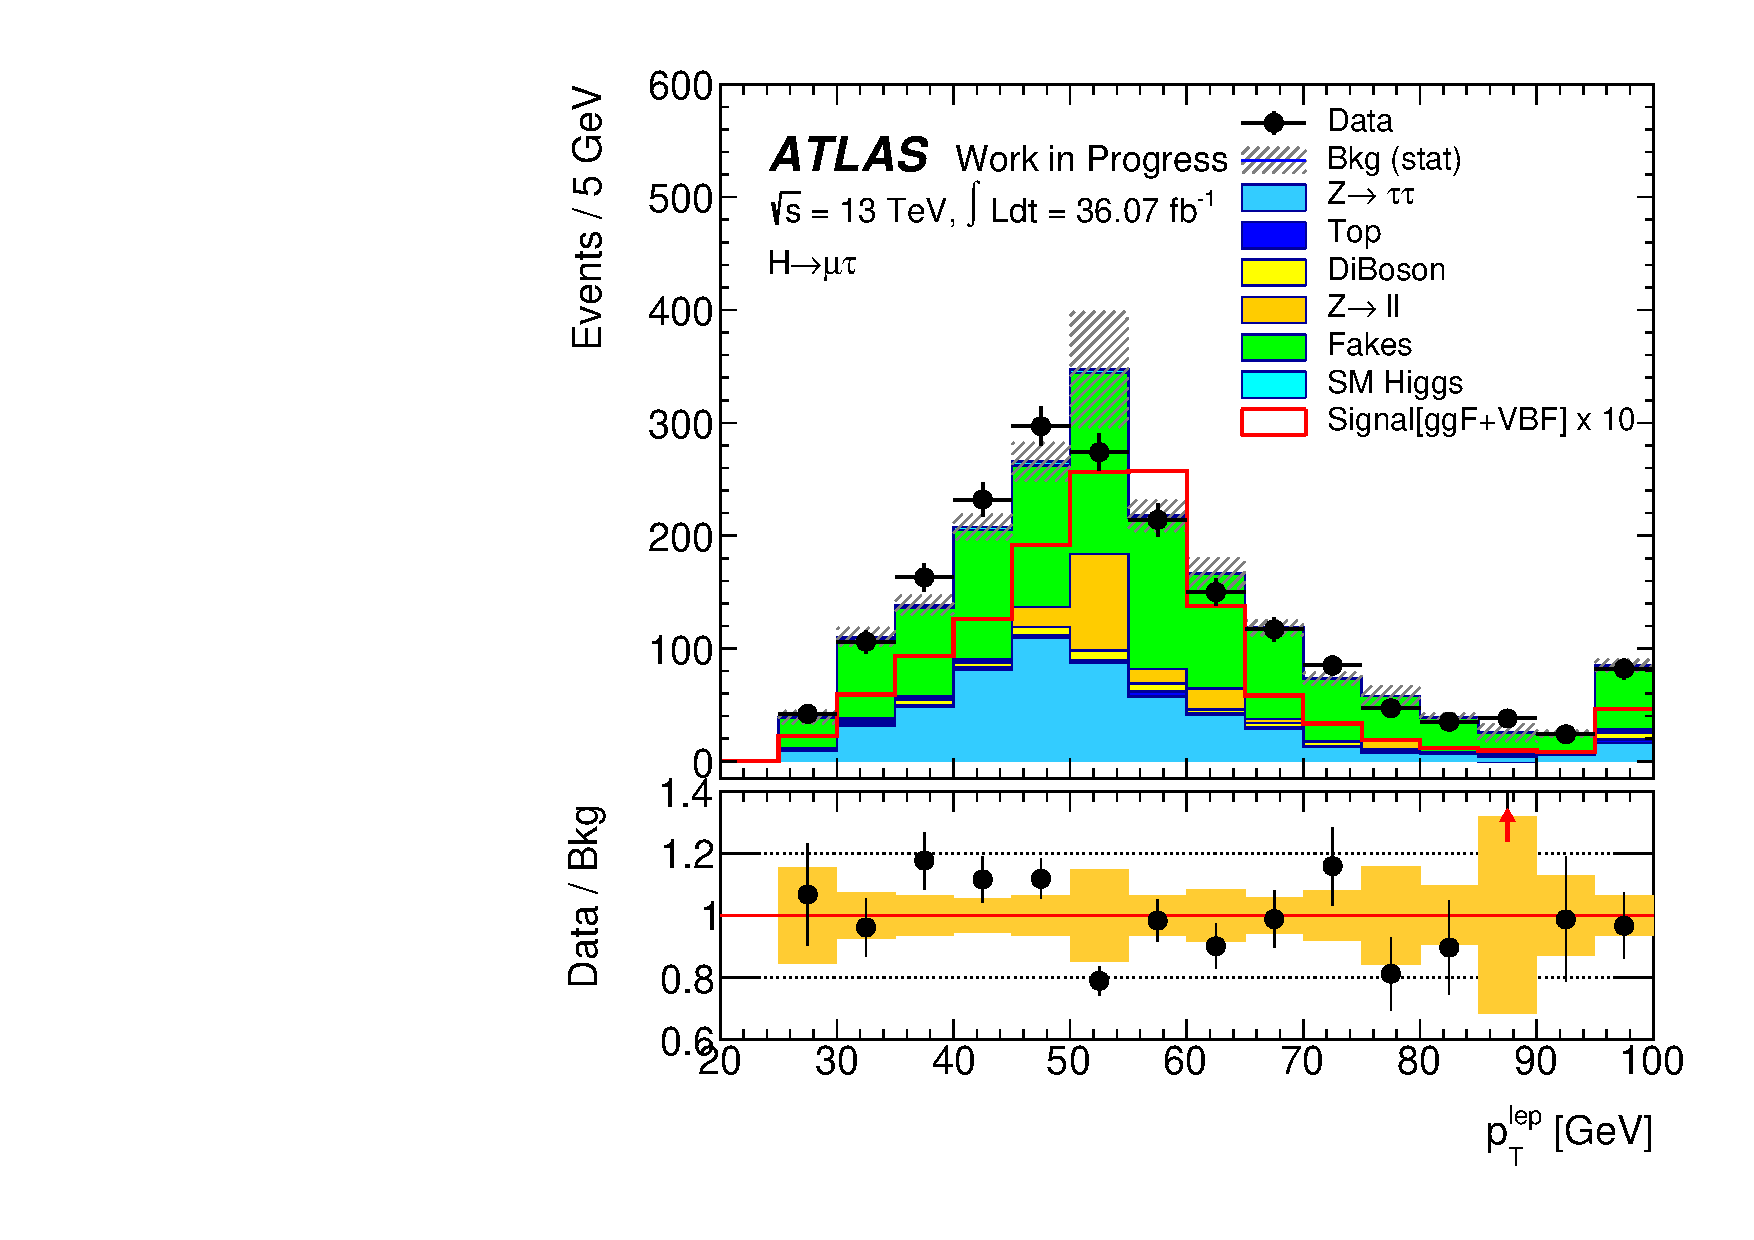
\includegraphics[width=.30\textwidth,height=.30\textheight,type=pdf,ext=.pdf,read=.pdf]{/afs/cern.ch/user/a/atpathak/afswork/public/Pixel/LFV_Plots/Plots_Qframework_25Apr2018_Final_note/plots_mcZll/mtau-CutTauMTSR2_Mvis-leptonPt-lin}
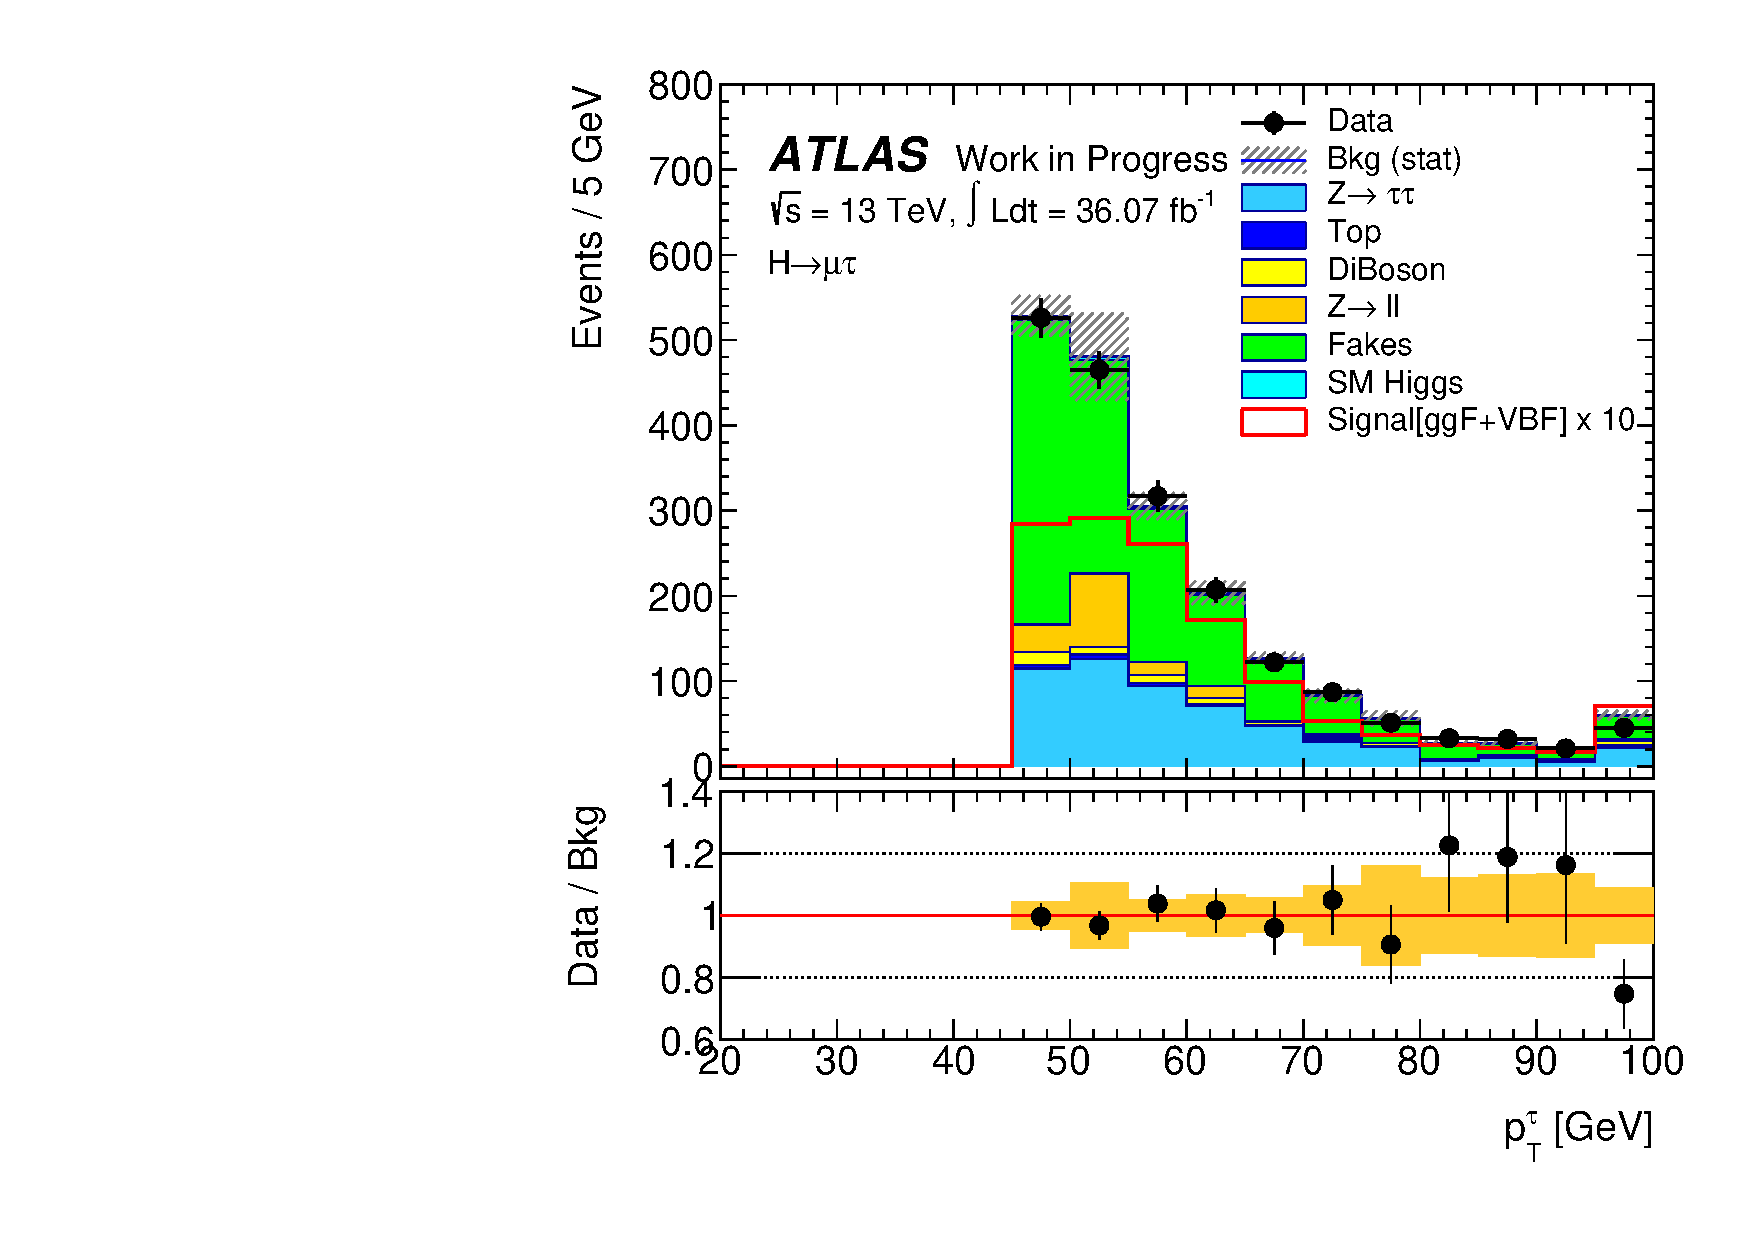
\includegraphics[width=.30\textwidth,height=.30\textheight,type=pdf,ext=.pdf,read=.pdf]{/afs/cern.ch/user/a/atpathak/afswork/public/Pixel/LFV_Plots/Plots_Qframework_25Apr2018_Final_note/plots_mcZll/mtau-CutTauMTSR2_Mvis-tauPt-lin}
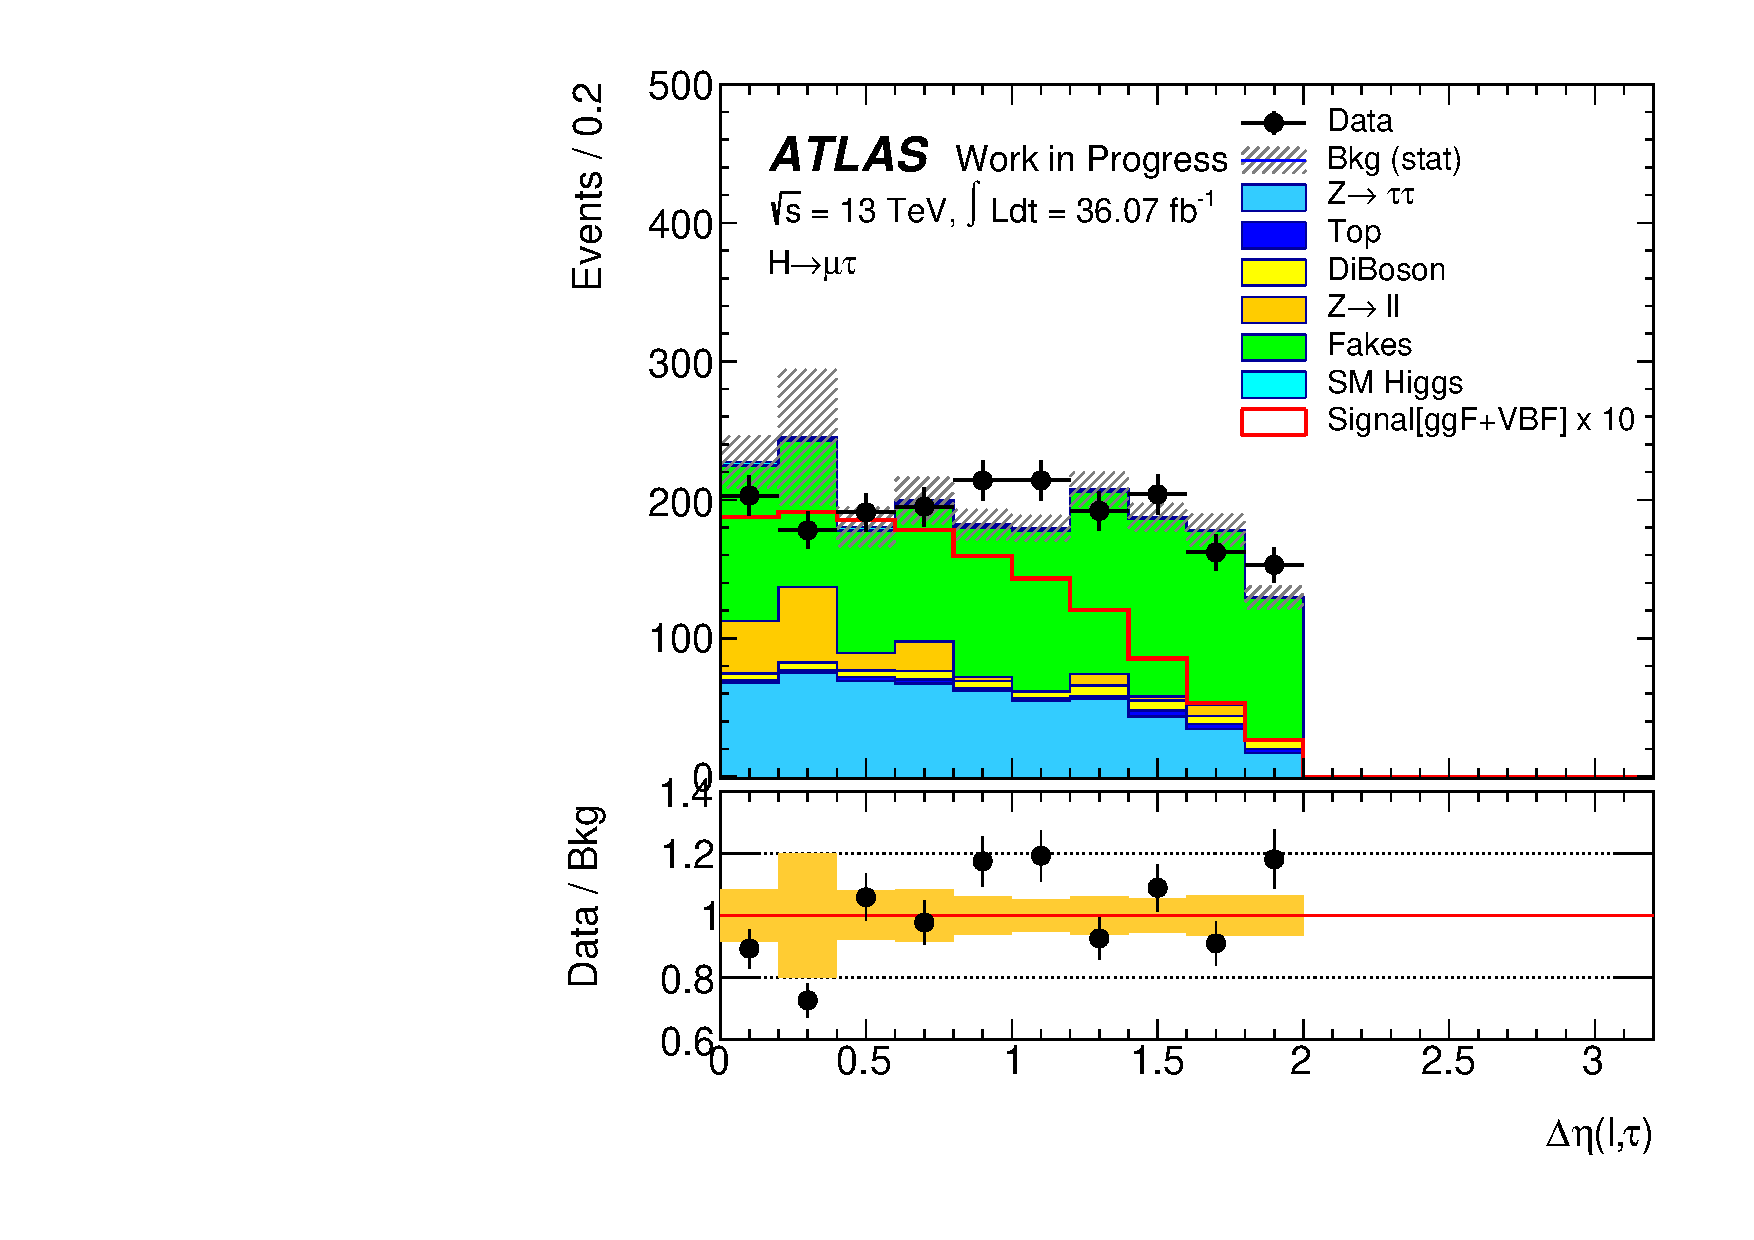
\includegraphics[width=.30\textwidth,height=.30\textheight,type=pdf,ext=.pdf,read=.pdf]{/afs/cern.ch/user/a/atpathak/afswork/public/Pixel/LFV_Plots/Plots_Qframework_25Apr2018_Final_note/plots_mcZll/mtau-CutTauMTSR2_Mvis-dEtaTauLep-lin}\\
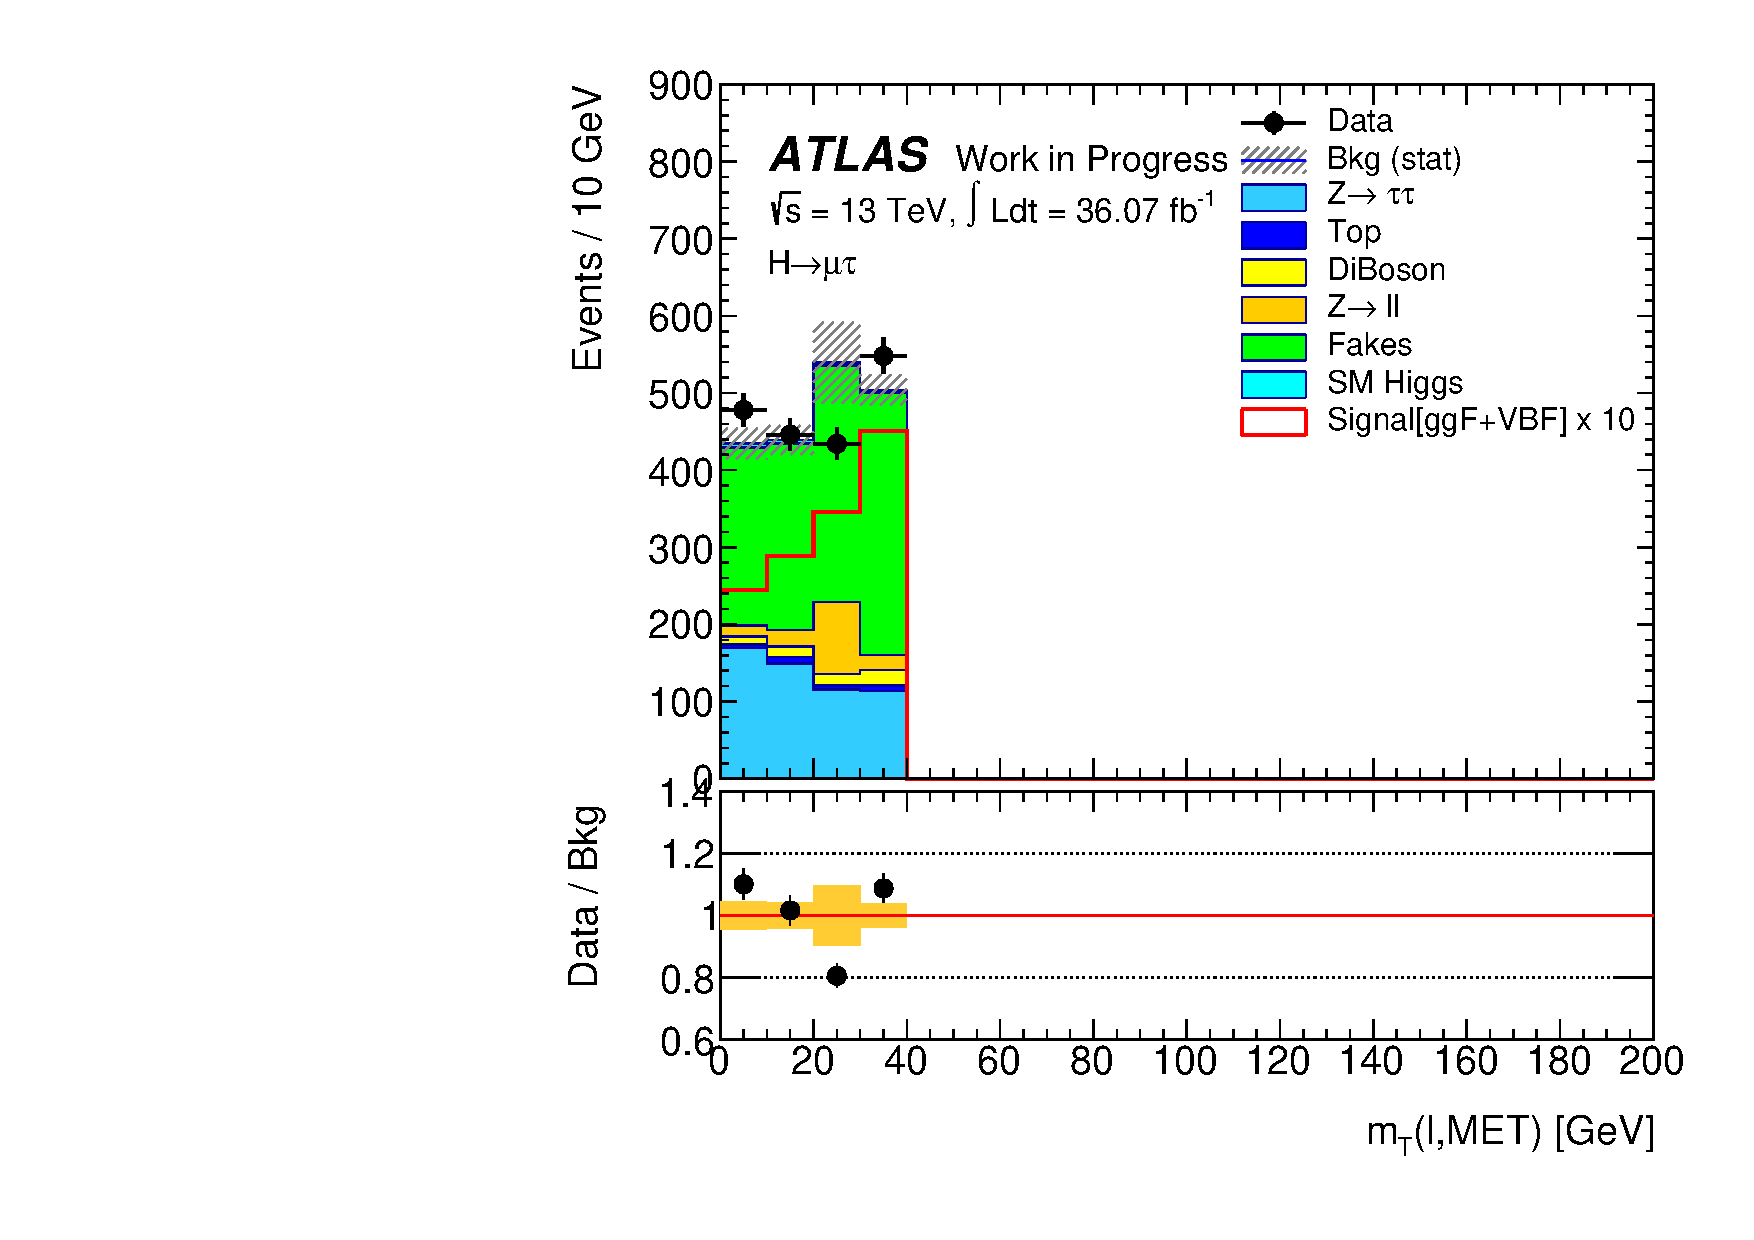
\includegraphics[width=.30\textwidth,height=.30\textheight,type=pdf,ext=.pdf,read=.pdf]{/afs/cern.ch/user/a/atpathak/afswork/public/Pixel/LFV_Plots/Plots_Qframework_25Apr2018_Final_note/plots_mcZll/mtau-CutTauMTSR2_Mvis-transverseMassLepMET-lin}
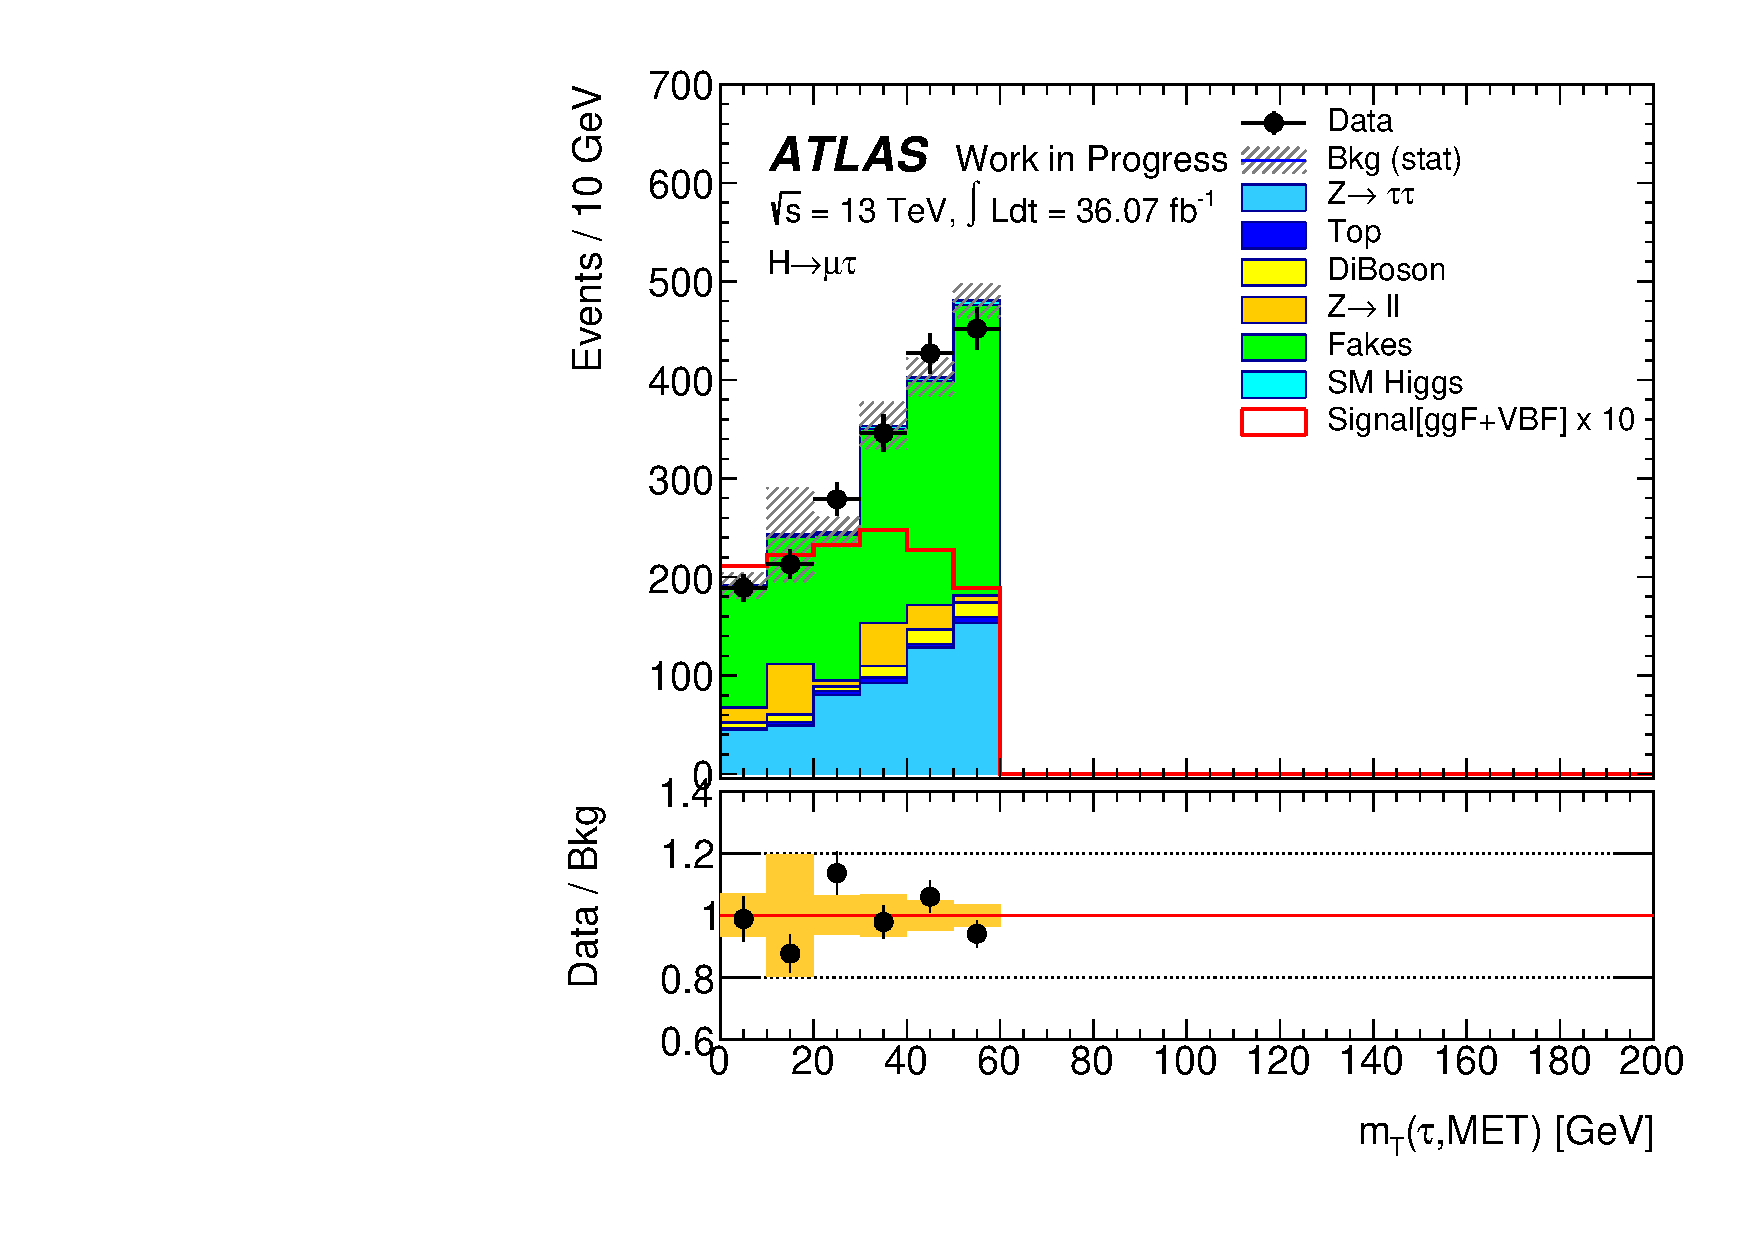
\includegraphics[width=.30\textwidth,height=.30\textheight,type=pdf,ext=.pdf,read=.pdf]{/afs/cern.ch/user/a/atpathak/afswork/public/Pixel/LFV_Plots/Plots_Qframework_25Apr2018_Final_note/plots_mcZll/mtau-CutTauMTSR2_Mvis-transverseMassTauMET-lin}
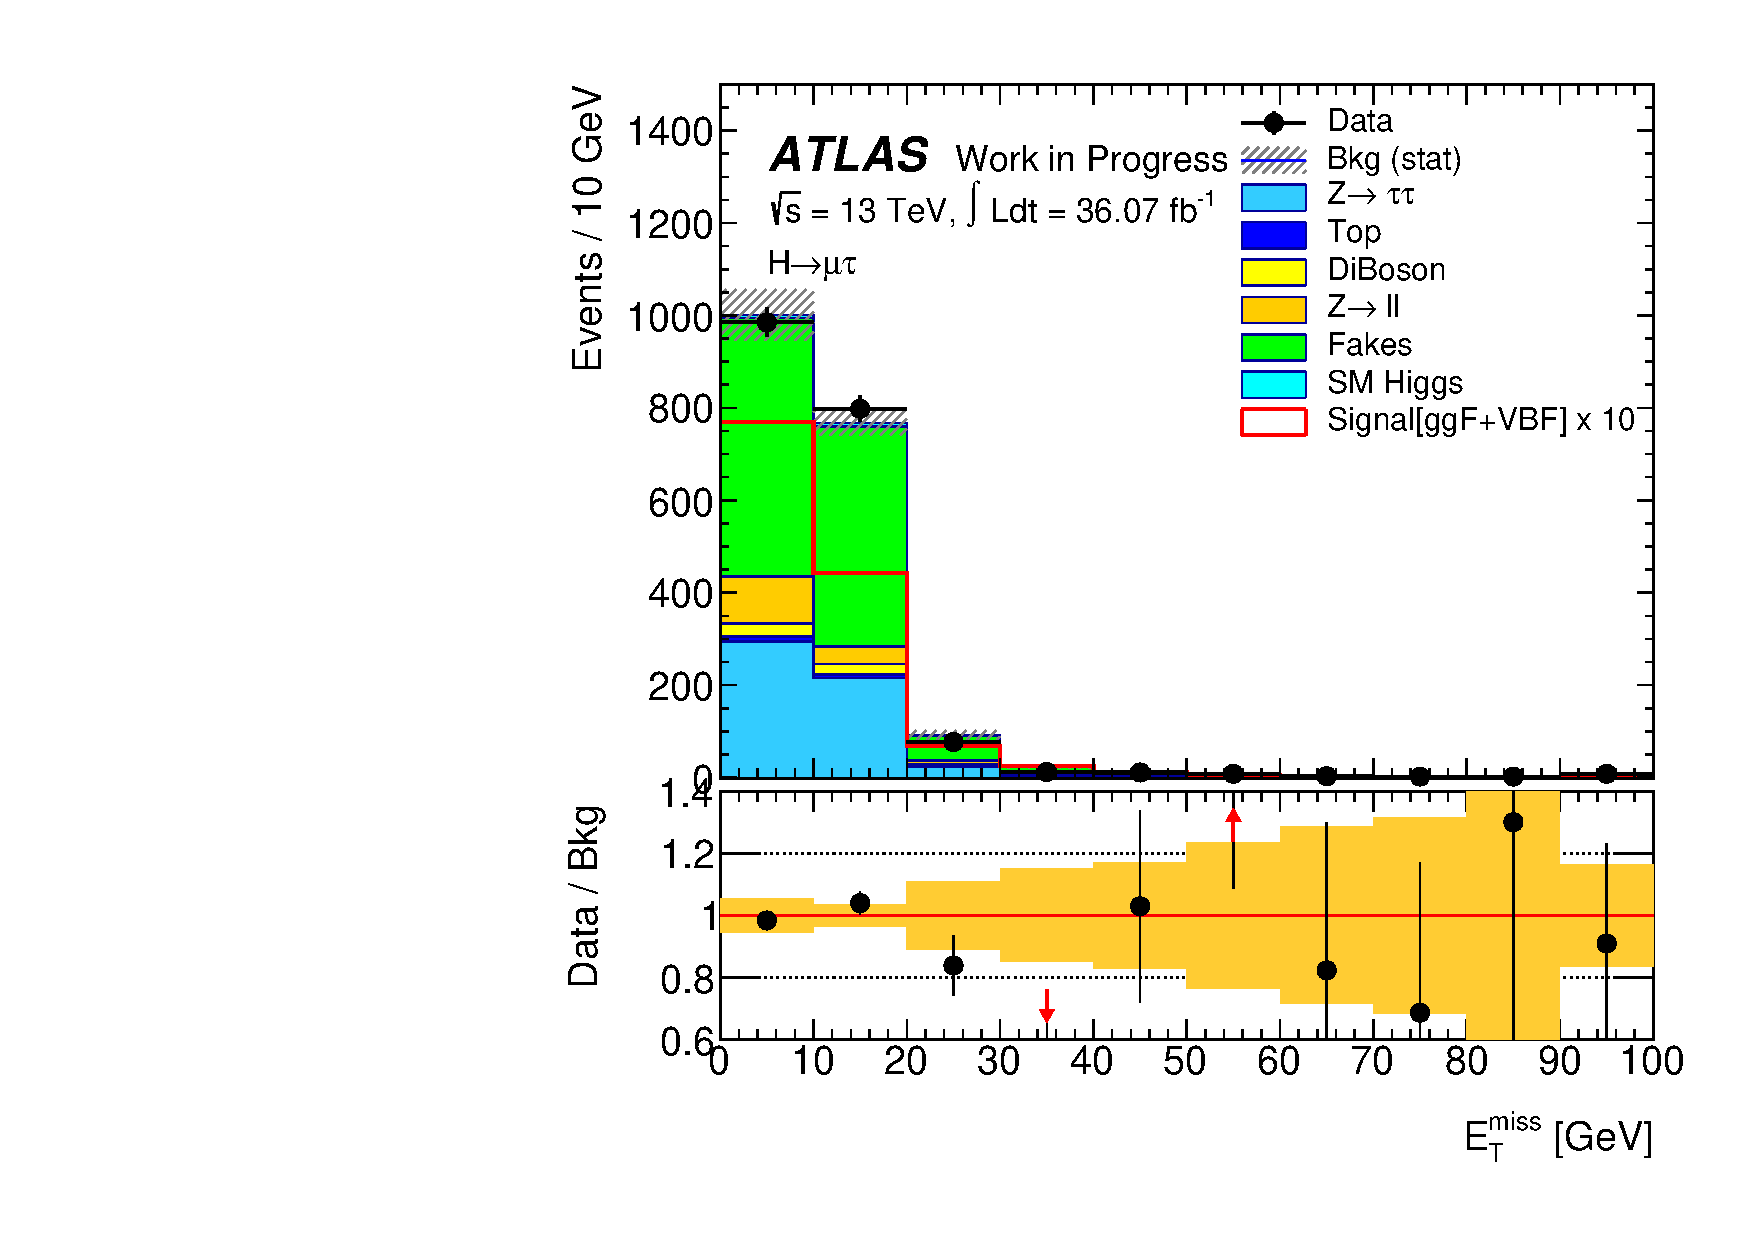
\includegraphics[width=.30\textwidth,height=.30\textheight,type=pdf,ext=.pdf,read=.pdf]{/afs/cern.ch/user/a/atpathak/afswork/public/Pixel/LFV_Plots/Plots_Qframework_25Apr2018_Final_note/plots_mcZll/mtau-CutTauMTSR2_Mvis-met-lin}\\
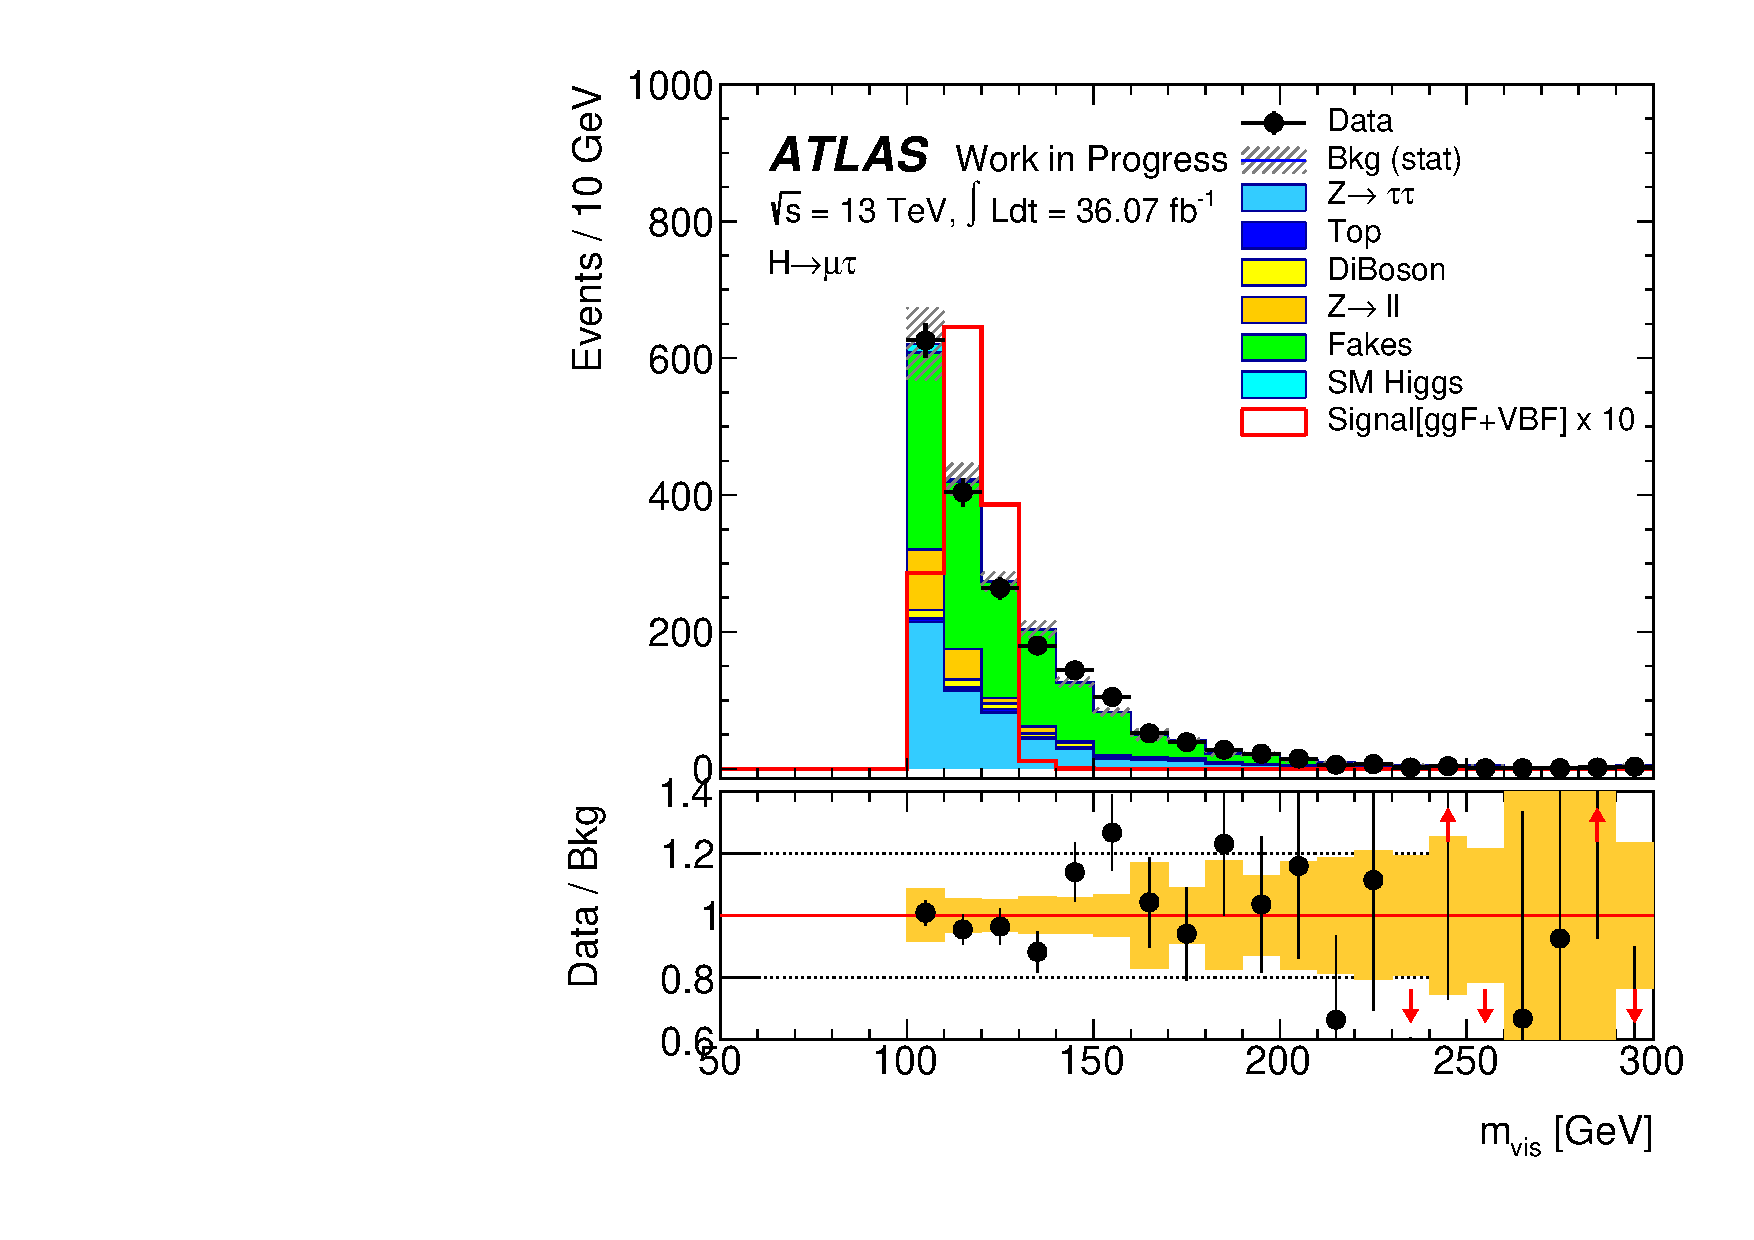
\includegraphics[width=.30\textwidth,height=.30\textheight,type=pdf,ext=.pdf,read=.pdf]{/afs/cern.ch/user/a/atpathak/afswork/public/Pixel/LFV_Plots/Plots_Qframework_25Apr2018_Final_note/plots_mcZll/mtau-CutTauMTSR2_Mvis-visibleMass-lin}
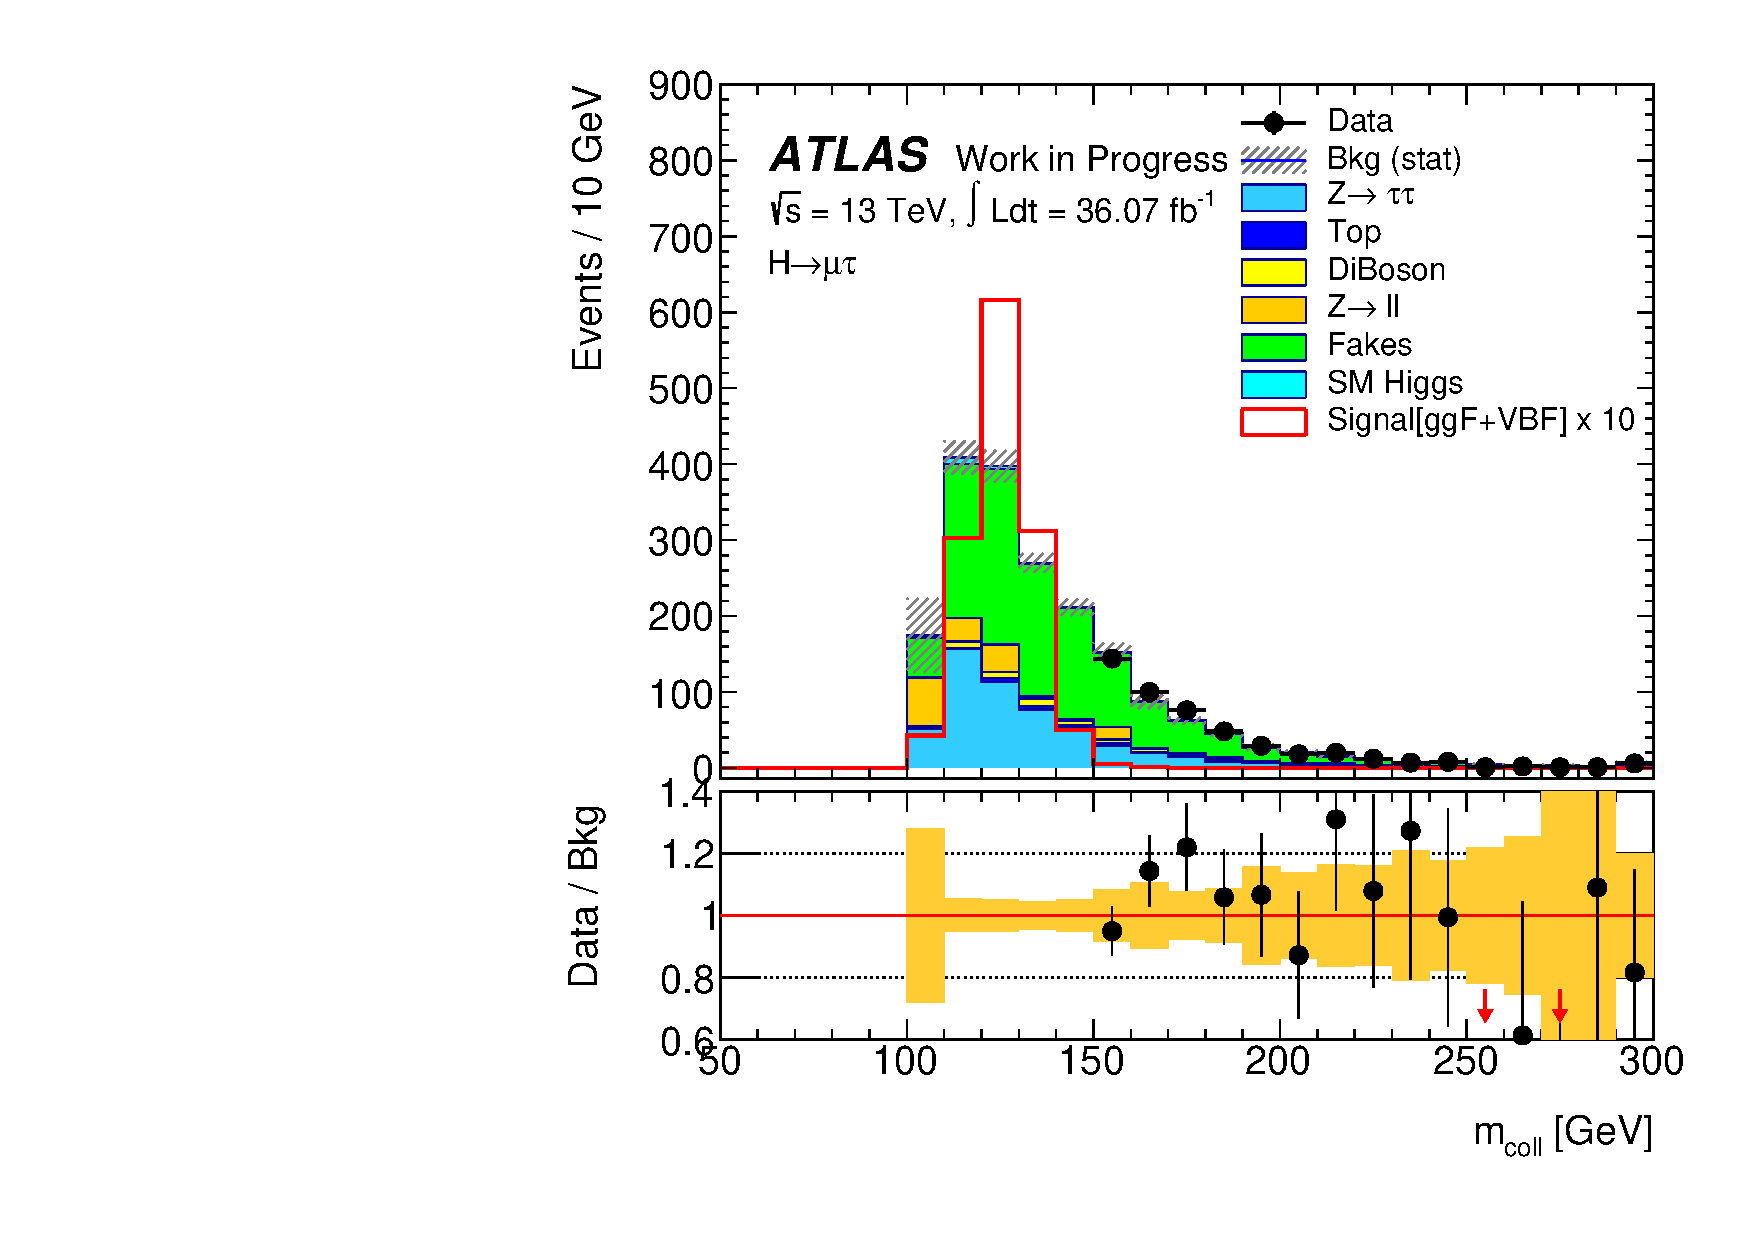
\includegraphics[width=.30\textwidth,height=.30\textheight,type=pdf,ext=.pdf,read=.pdf]{/afs/cern.ch/user/a/atpathak/afswork/public/Pixel/LFV_Plots/Plots_Qframework_25Apr2018_Final_note/plots_mcZll/mtau-CutTauMTSR2_Mvis-collMassBL-lin}
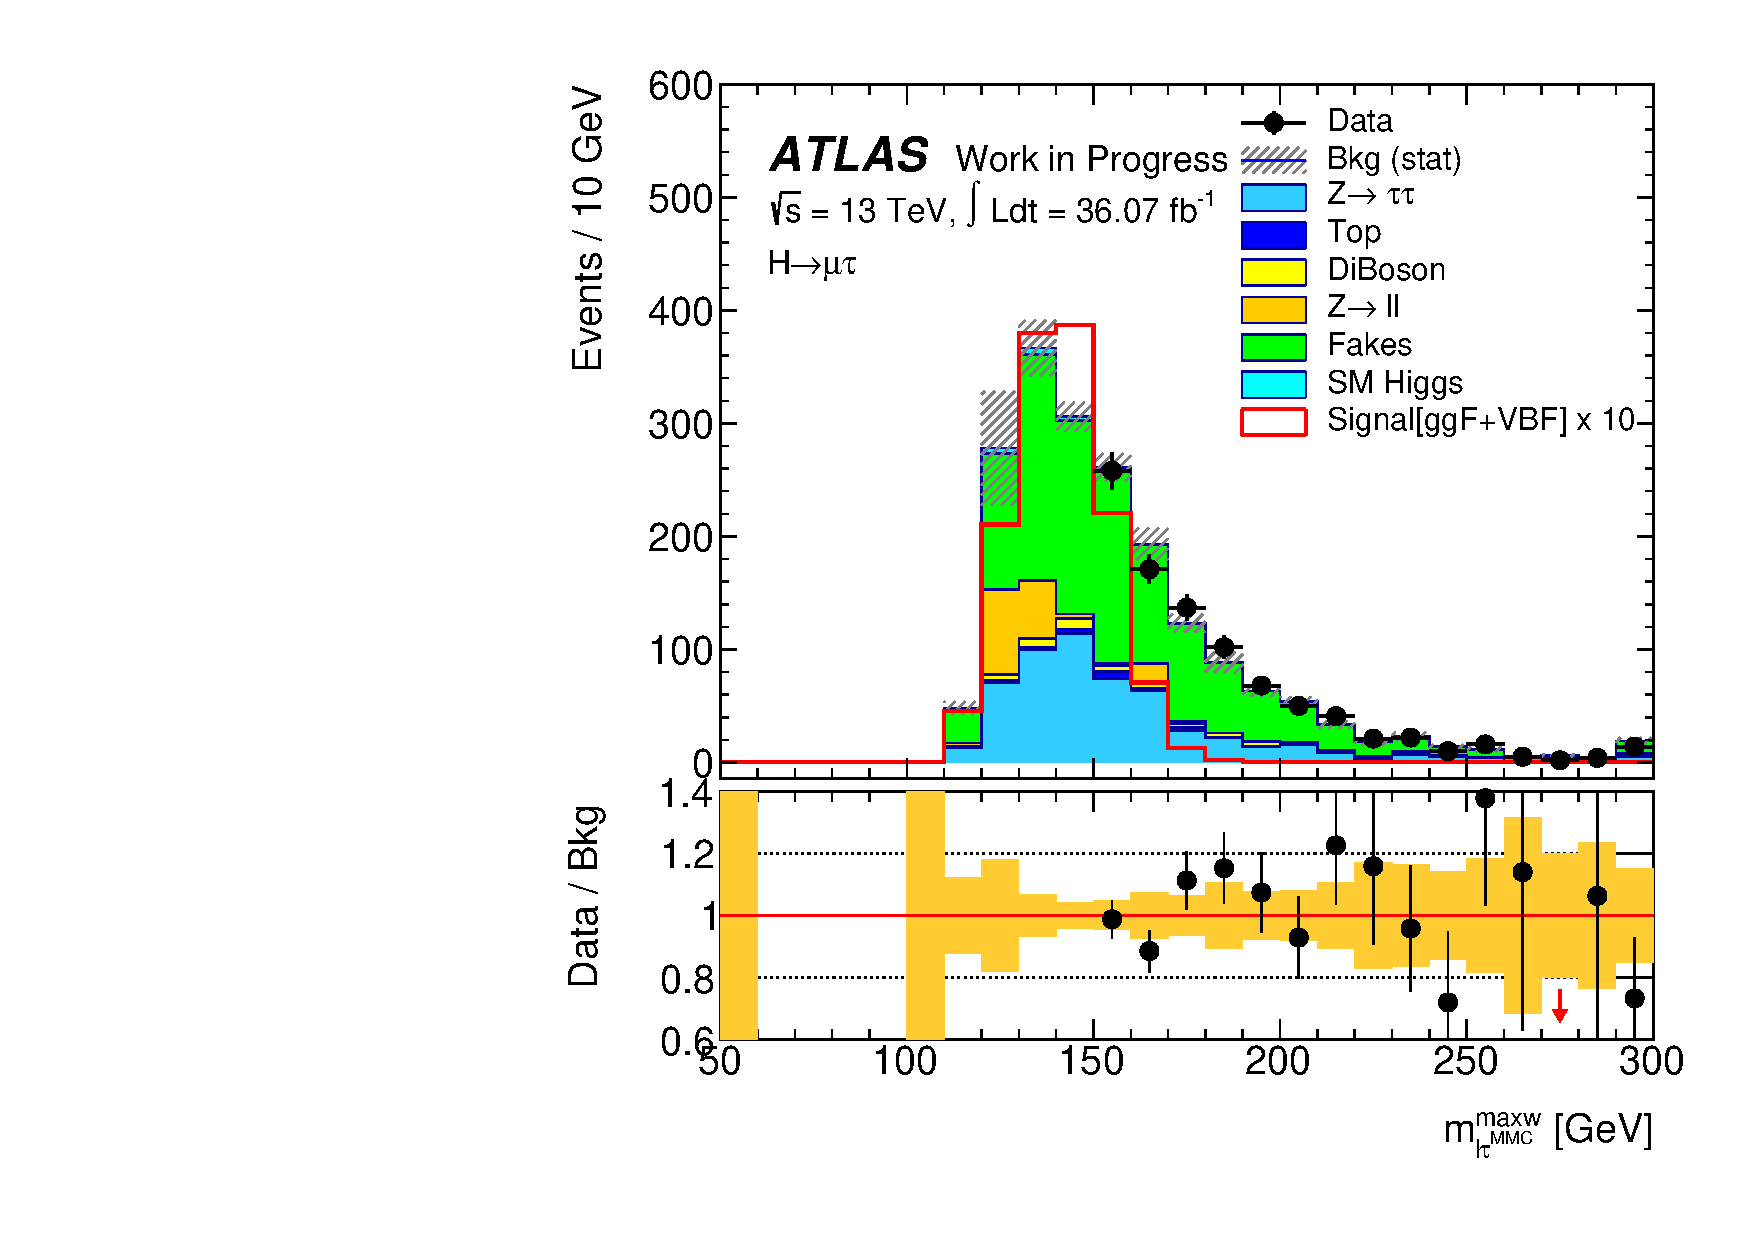
\includegraphics[width=.30\textwidth,height=.30\textheight,type=pdf,ext=.pdf,read=.pdf]{/afs/cern.ch/user/a/atpathak/afswork/public/Pixel/LFV_Plots/Plots_Qframework_25Apr2018_Final_note/plots_mcZll/mtau-CutTauMTSR2_Mvis-MMCBL-lin}
\end{normalsize}
\end{frame}
%-----------------------------------------------
\begin{frame}
\frametitle{Distributions of $\mu\tau_{had}$ events in the SR3 region.}
\begin{normalsize}
\vspace*{0.2cm}
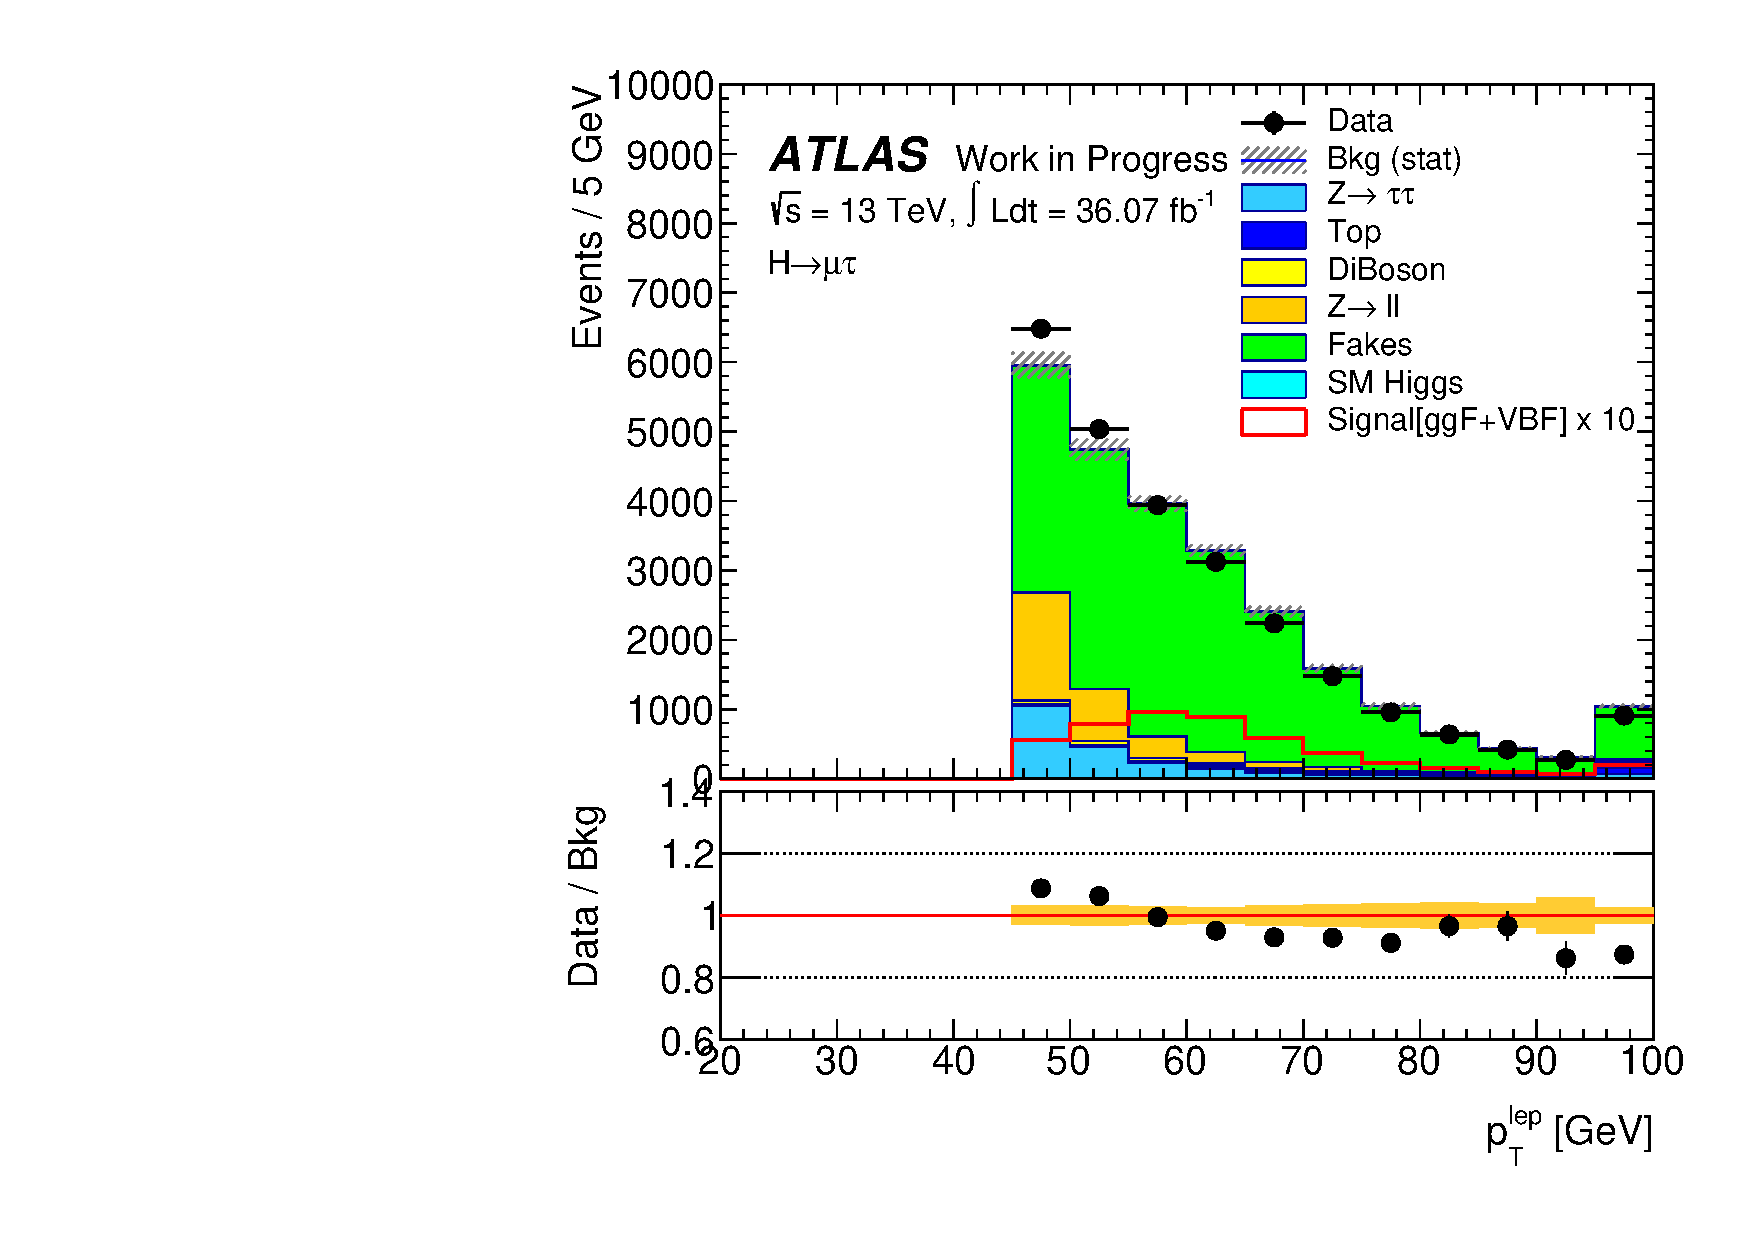
\includegraphics[width=.30\textwidth,height=.30\textheight,type=pdf,ext=.pdf,read=.pdf]{/afs/cern.ch/user/a/atpathak/afswork/public/Pixel/LFV_Plots/Plots_Qframework_25Apr2018_Final_note/plots_mcZll/mtau-CutTauPtSR3-leptonPt-lin}
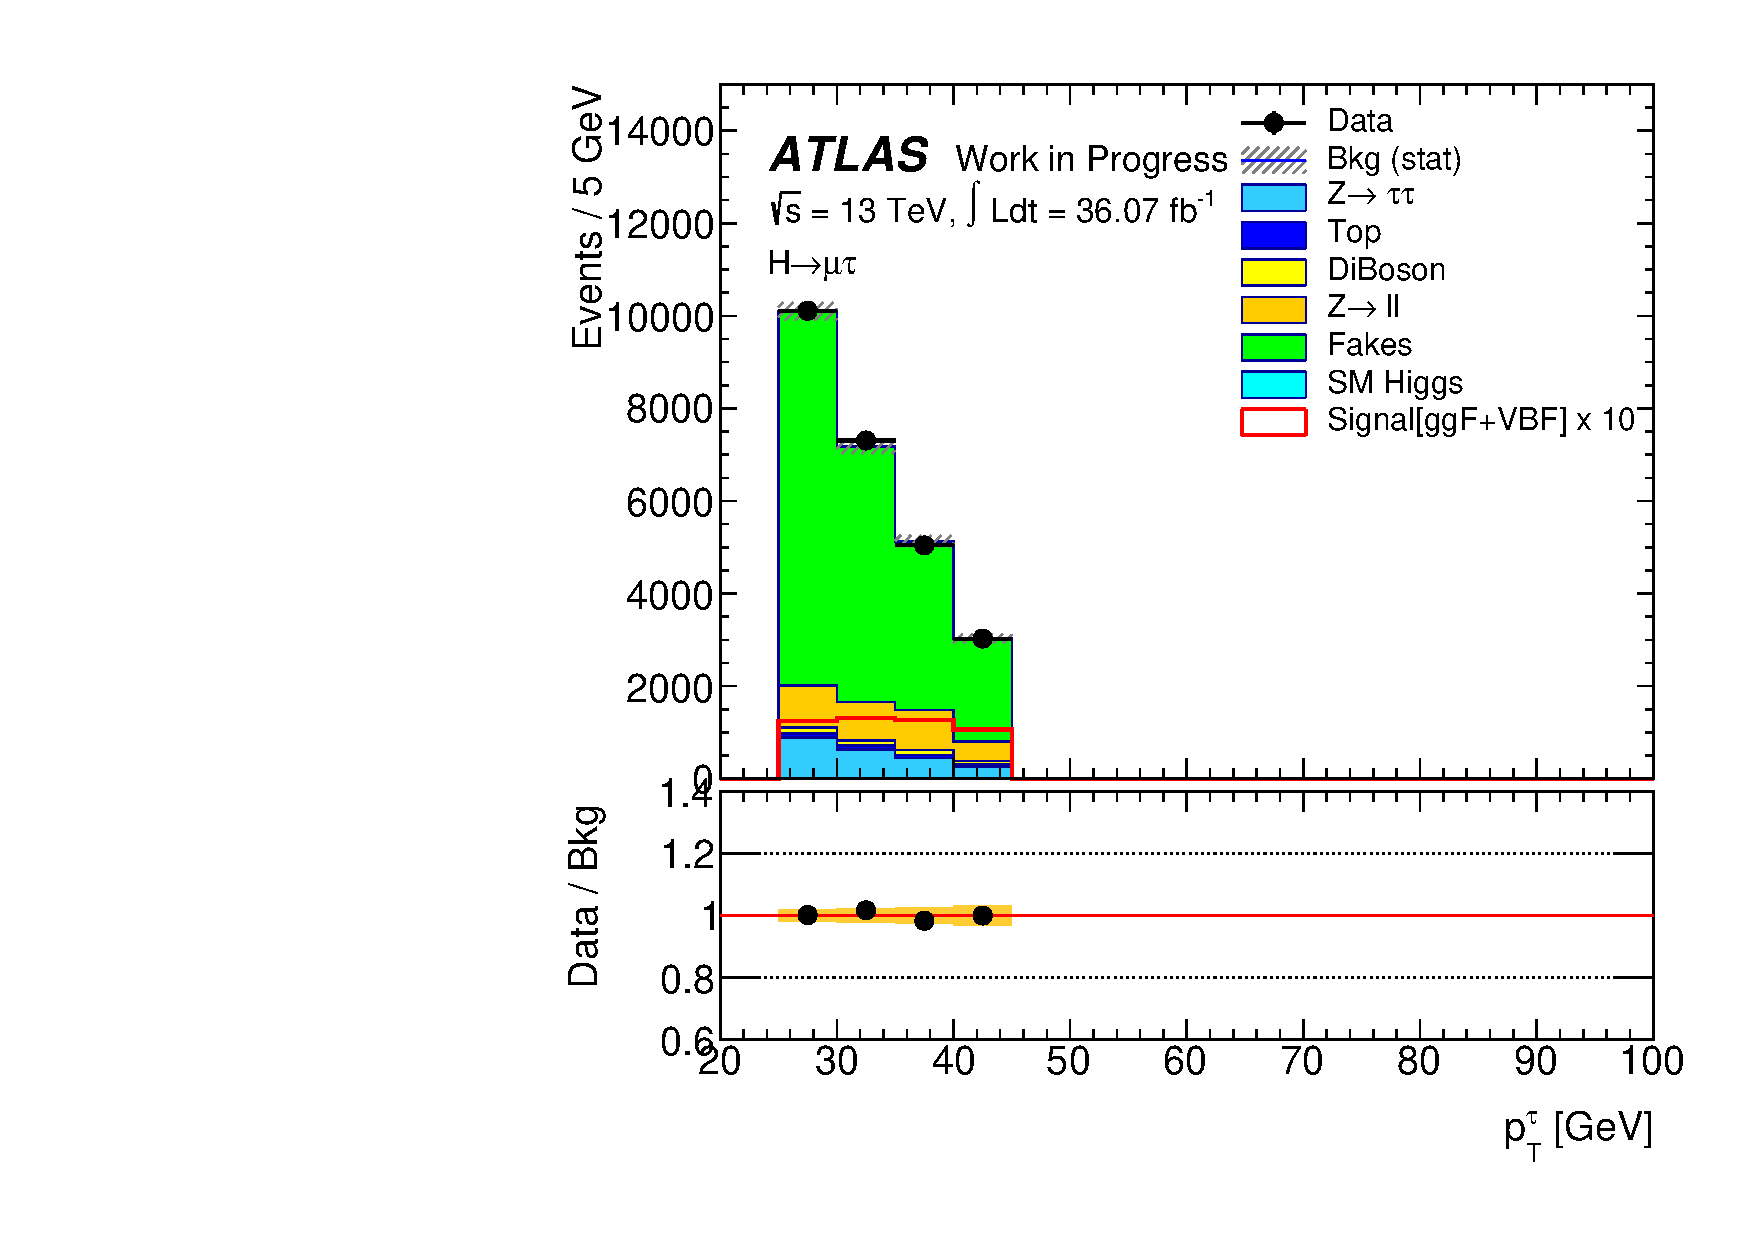
\includegraphics[width=.30\textwidth,height=.30\textheight,type=pdf,ext=.pdf,read=.pdf]{/afs/cern.ch/user/a/atpathak/afswork/public/Pixel/LFV_Plots/Plots_Qframework_25Apr2018_Final_note/plots_mcZll/mtau-CutTauPtSR3-tauPt-lin}
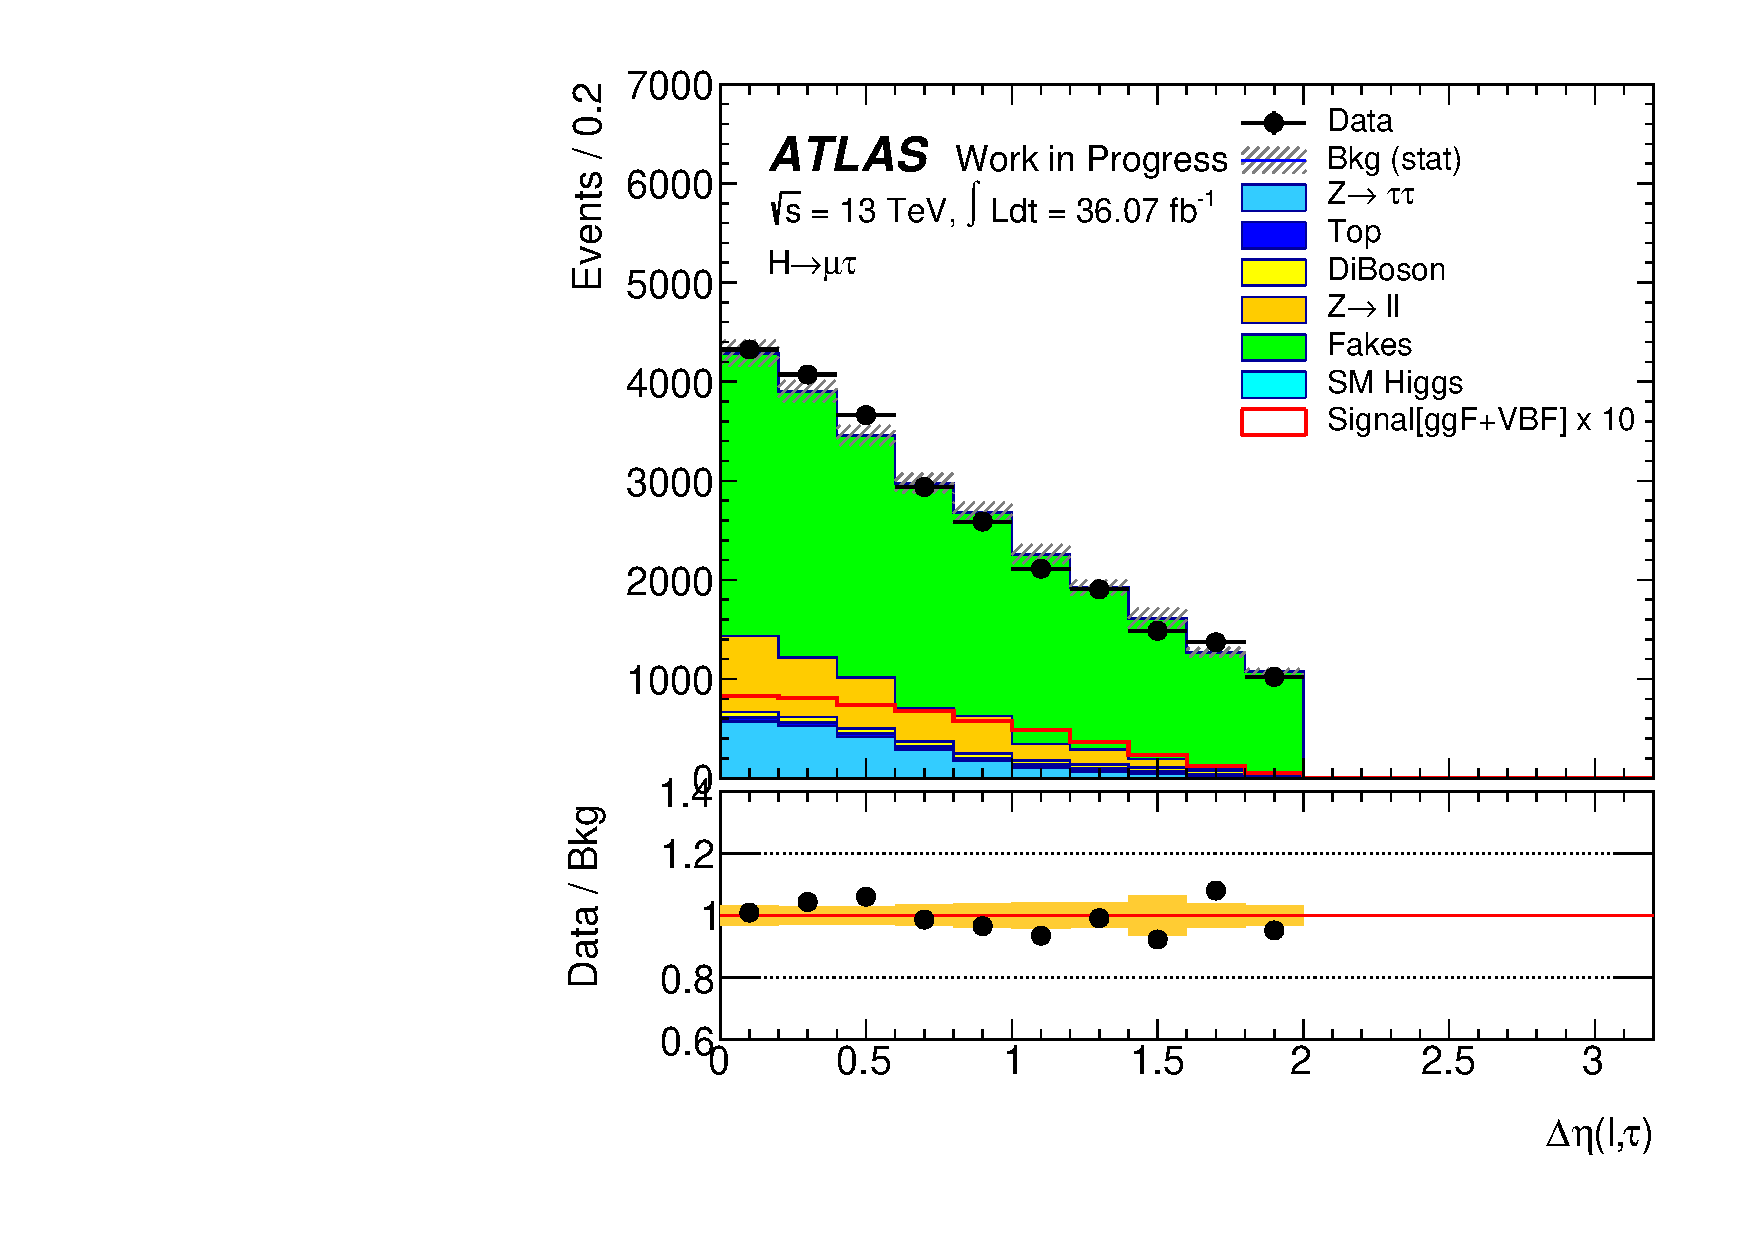
\includegraphics[width=.30\textwidth,height=.30\textheight,type=pdf,ext=.pdf,read=.pdf]{/afs/cern.ch/user/a/atpathak/afswork/public/Pixel/LFV_Plots/Plots_Qframework_25Apr2018_Final_note/plots_mcZll/mtau-CutTauPtSR3-dEtaTauLep-lin}\\
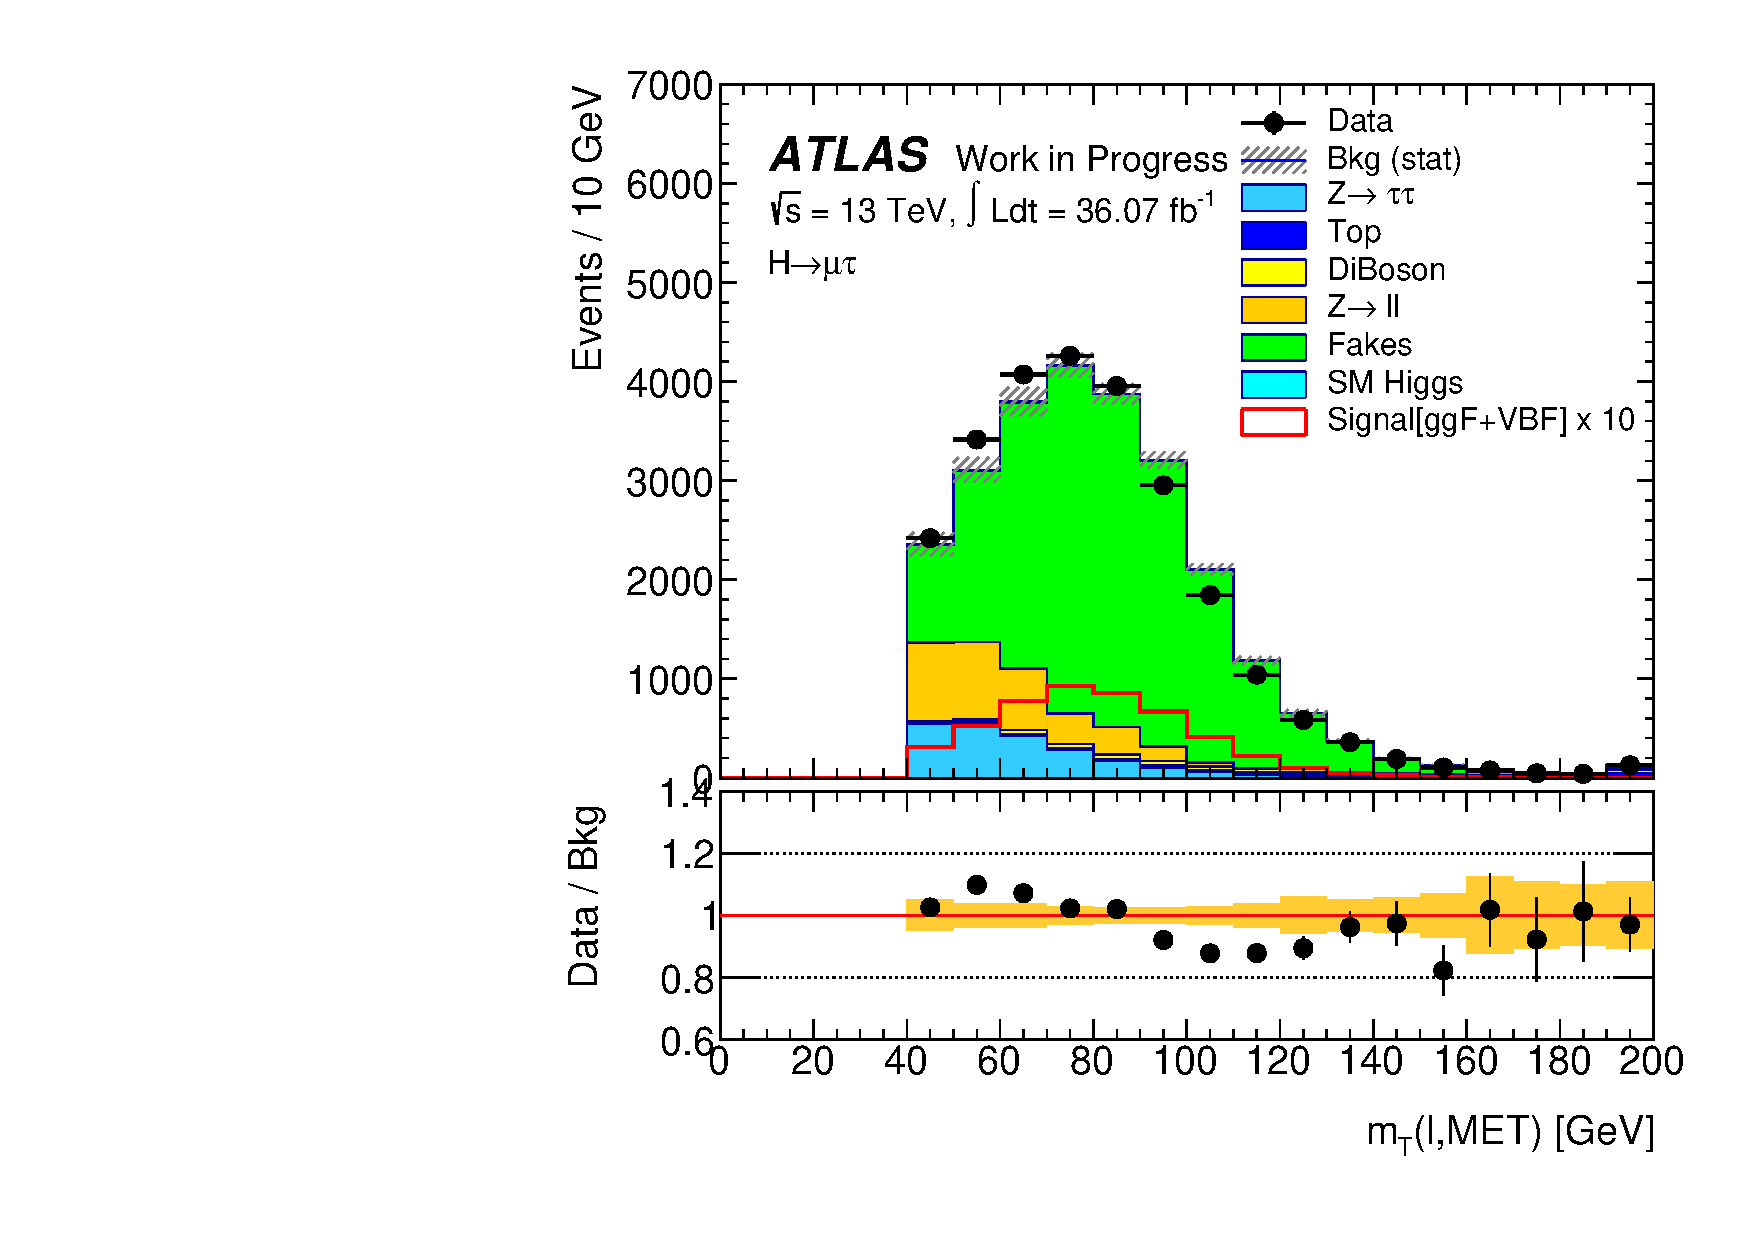
\includegraphics[width=.30\textwidth,height=.30\textheight,type=pdf,ext=.pdf,read=.pdf]{/afs/cern.ch/user/a/atpathak/afswork/public/Pixel/LFV_Plots/Plots_Qframework_25Apr2018_Final_note/plots_mcZll/mtau-CutTauPtSR3-transverseMassLepMET-lin}
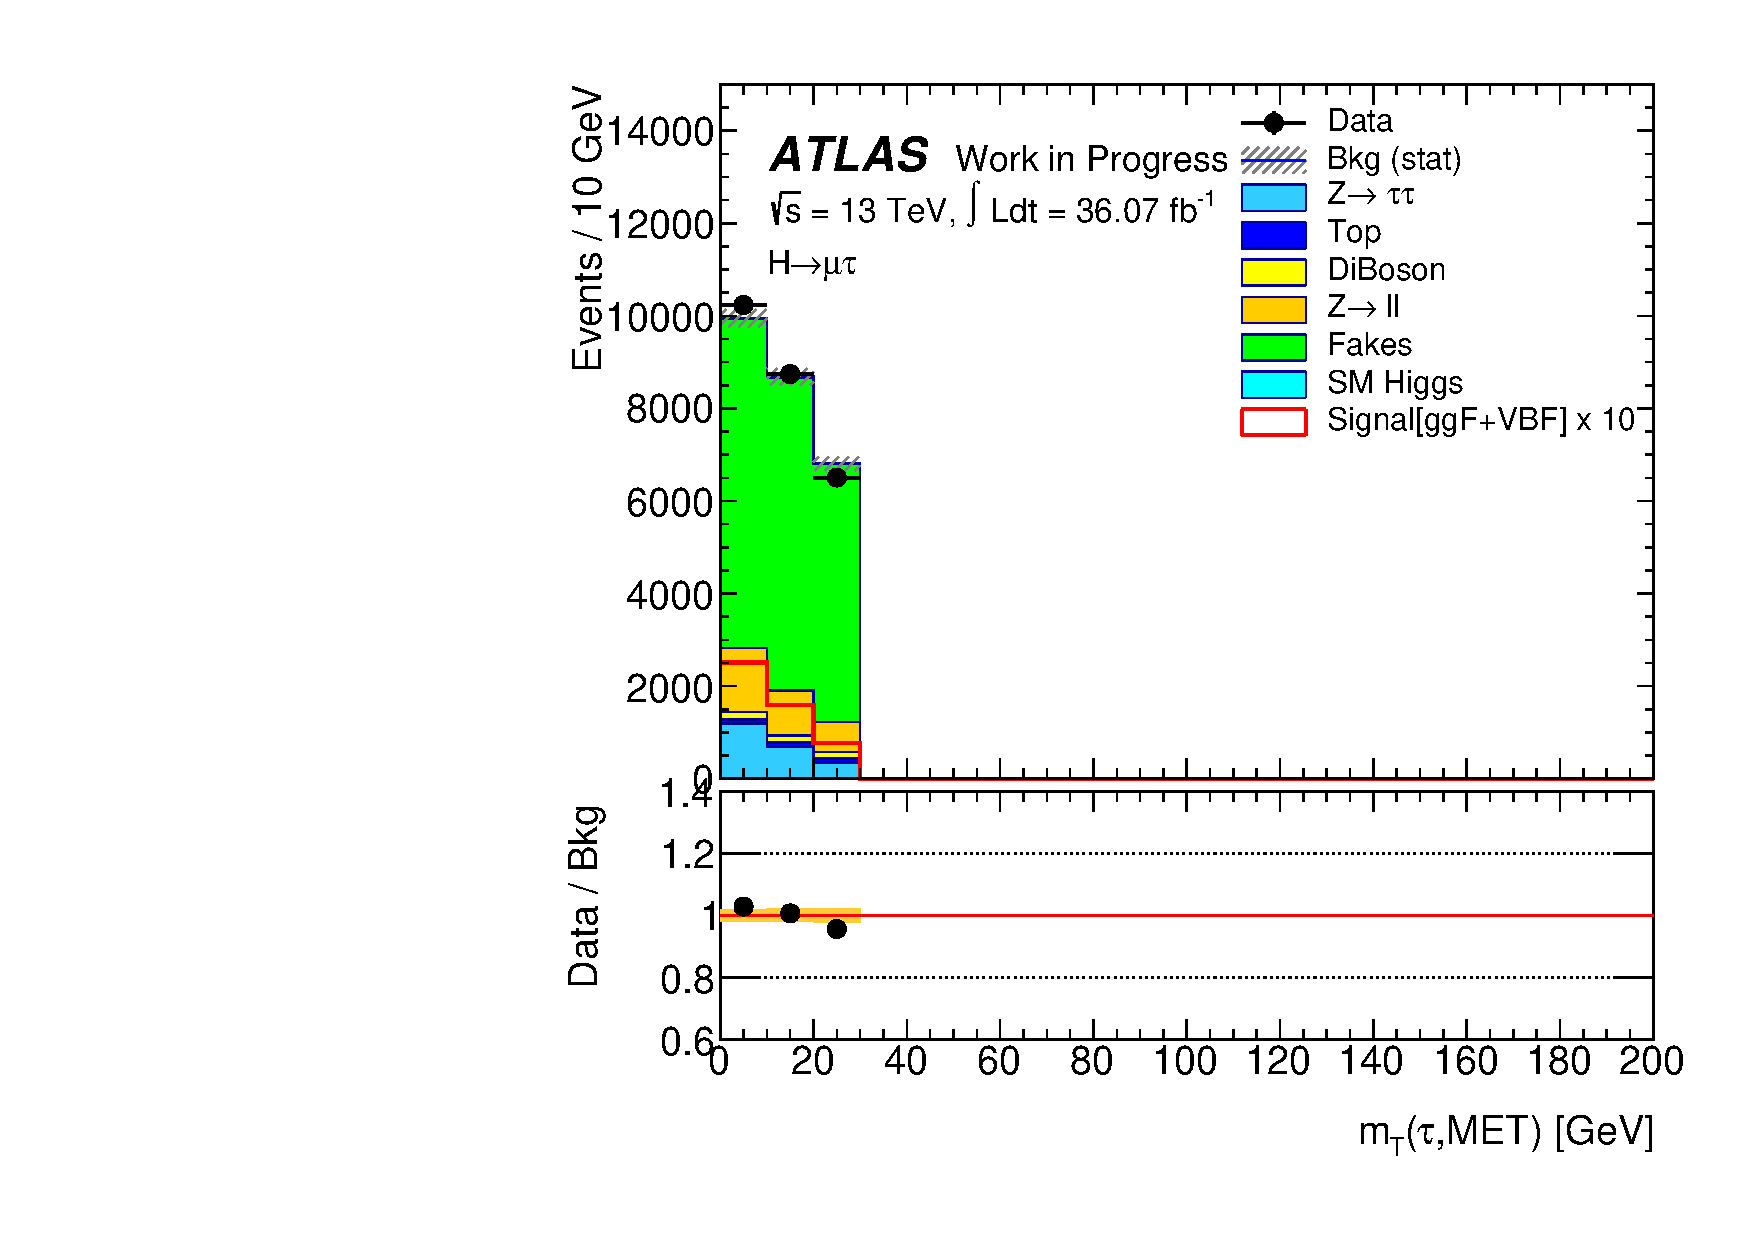
\includegraphics[width=.30\textwidth,height=.30\textheight,type=pdf,ext=.pdf,read=.pdf]{/afs/cern.ch/user/a/atpathak/afswork/public/Pixel/LFV_Plots/Plots_Qframework_25Apr2018_Final_note/plots_mcZll/mtau-CutTauPtSR3-transverseMassTauMET-lin}
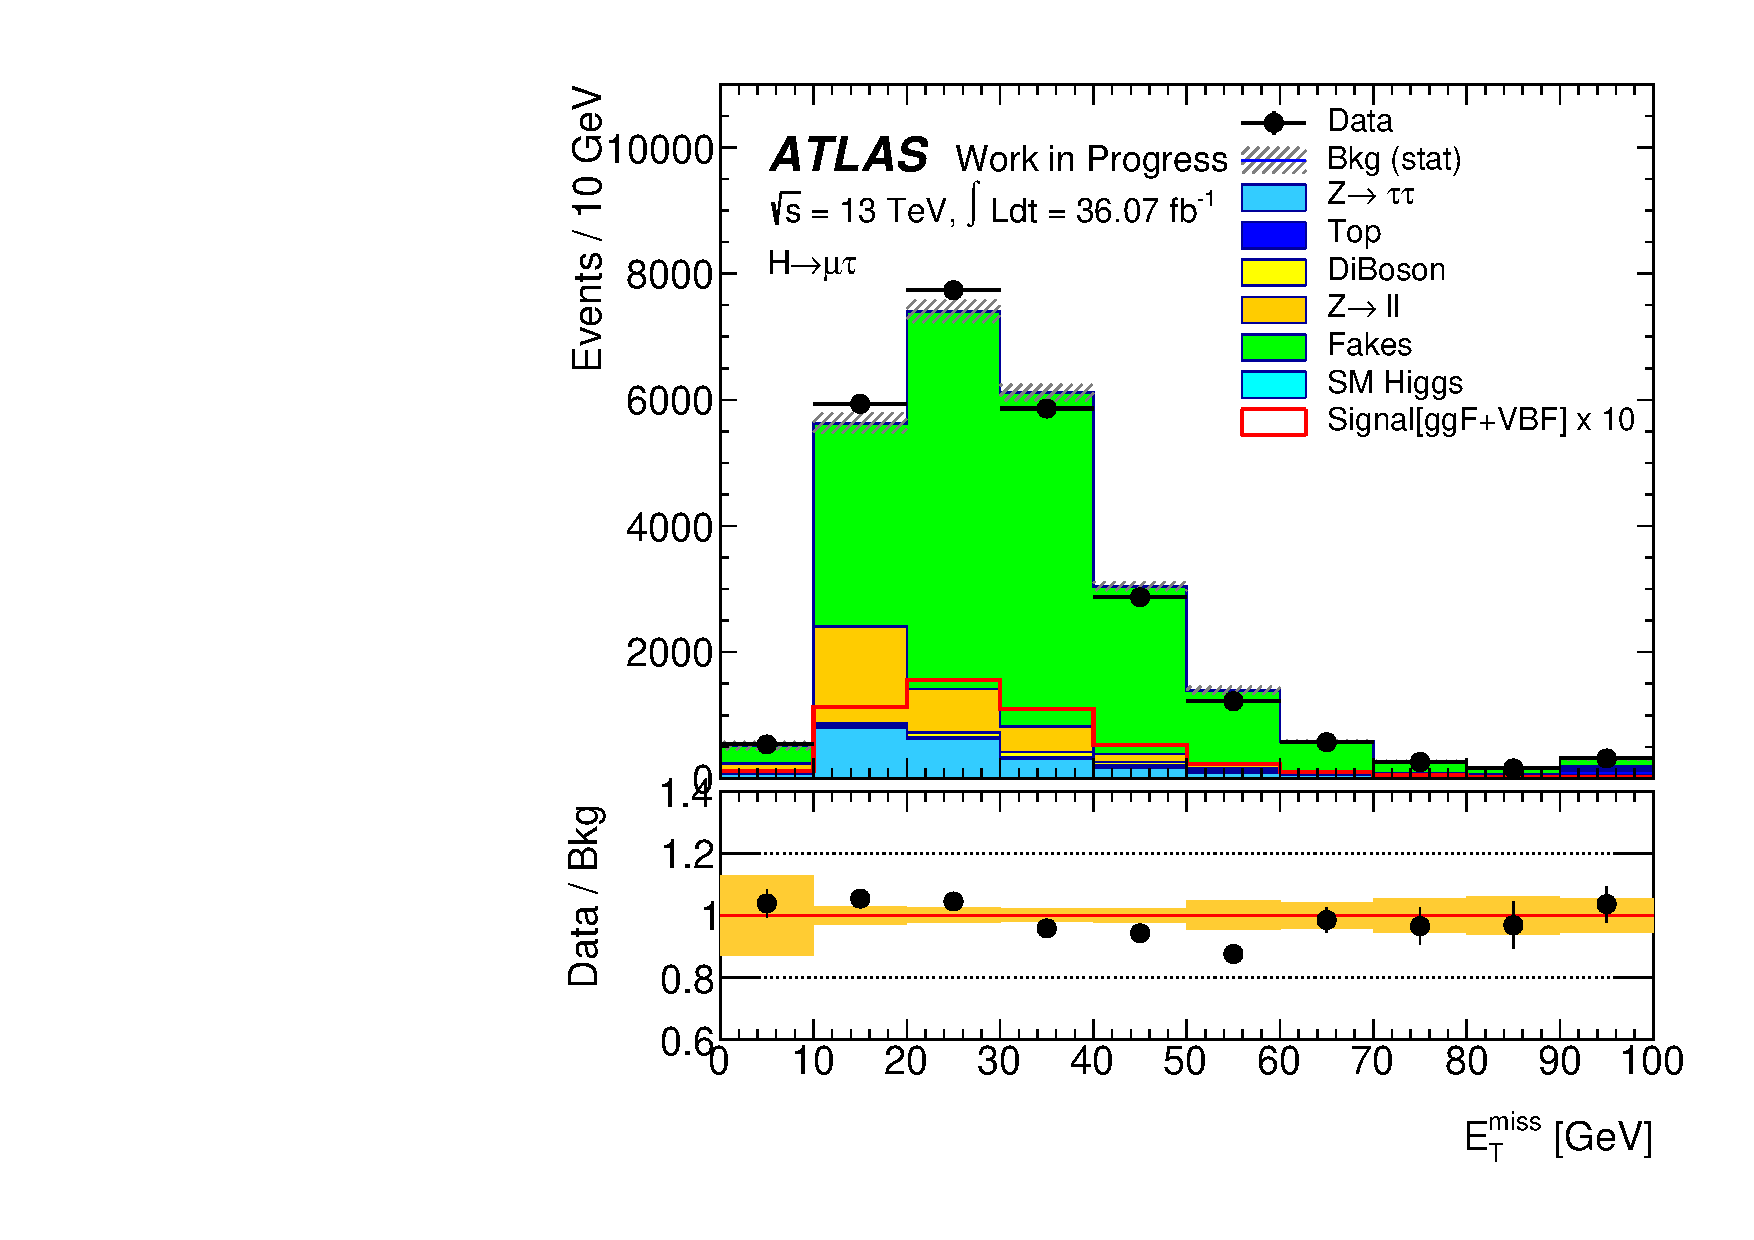
\includegraphics[width=.30\textwidth,height=.30\textheight,type=pdf,ext=.pdf,read=.pdf]{/afs/cern.ch/user/a/atpathak/afswork/public/Pixel/LFV_Plots/Plots_Qframework_25Apr2018_Final_note/plots_mcZll/mtau-CutTauPtSR3-met-lin}\\
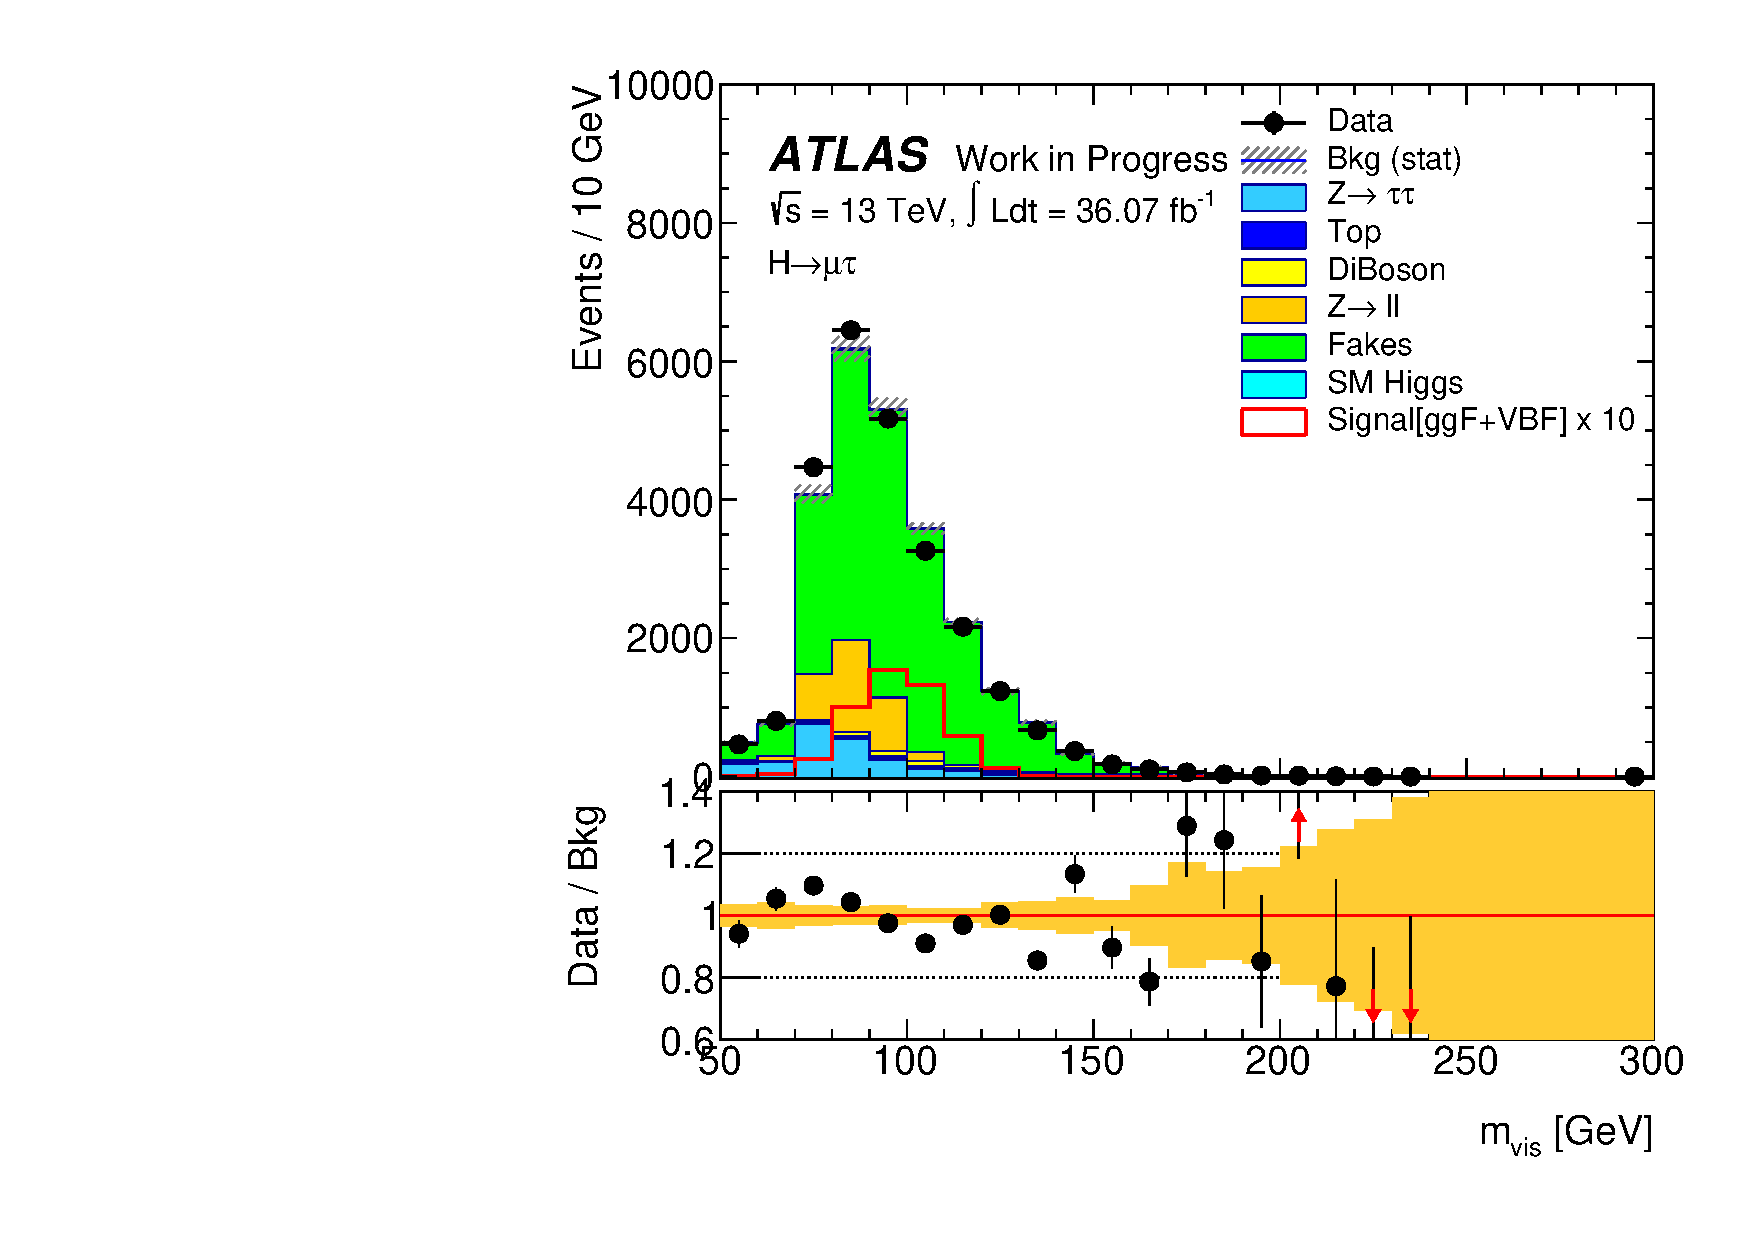
\includegraphics[width=.30\textwidth,height=.30\textheight,type=pdf,ext=.pdf,read=.pdf]{/afs/cern.ch/user/a/atpathak/afswork/public/Pixel/LFV_Plots/Plots_Qframework_25Apr2018_Final_note/plots_mcZll/mtau-CutTauPtSR3-visibleMass-lin}
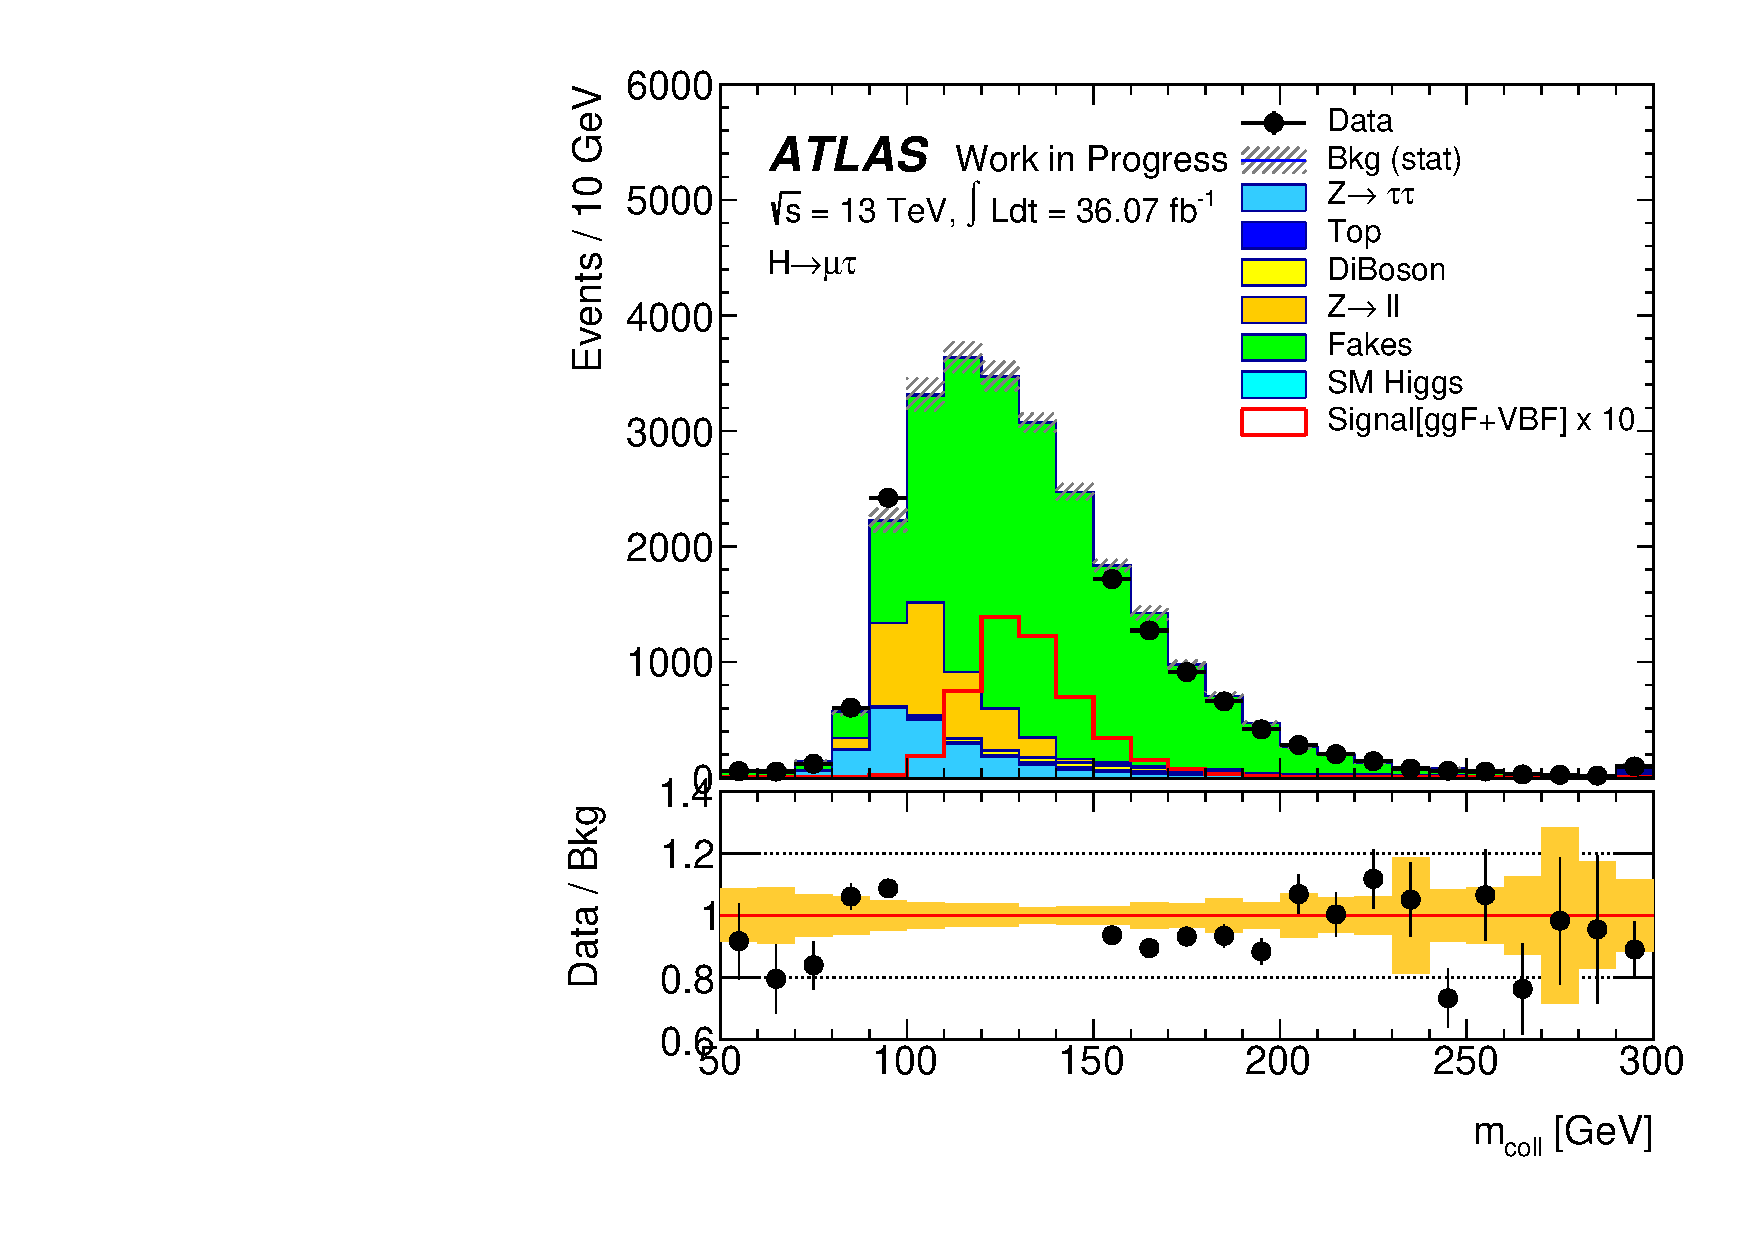
\includegraphics[width=.30\textwidth,height=.30\textheight,type=pdf,ext=.pdf,read=.pdf]{/afs/cern.ch/user/a/atpathak/afswork/public/Pixel/LFV_Plots/Plots_Qframework_25Apr2018_Final_note/plots_mcZll/mtau-CutTauPtSR3-collMassBL-lin}
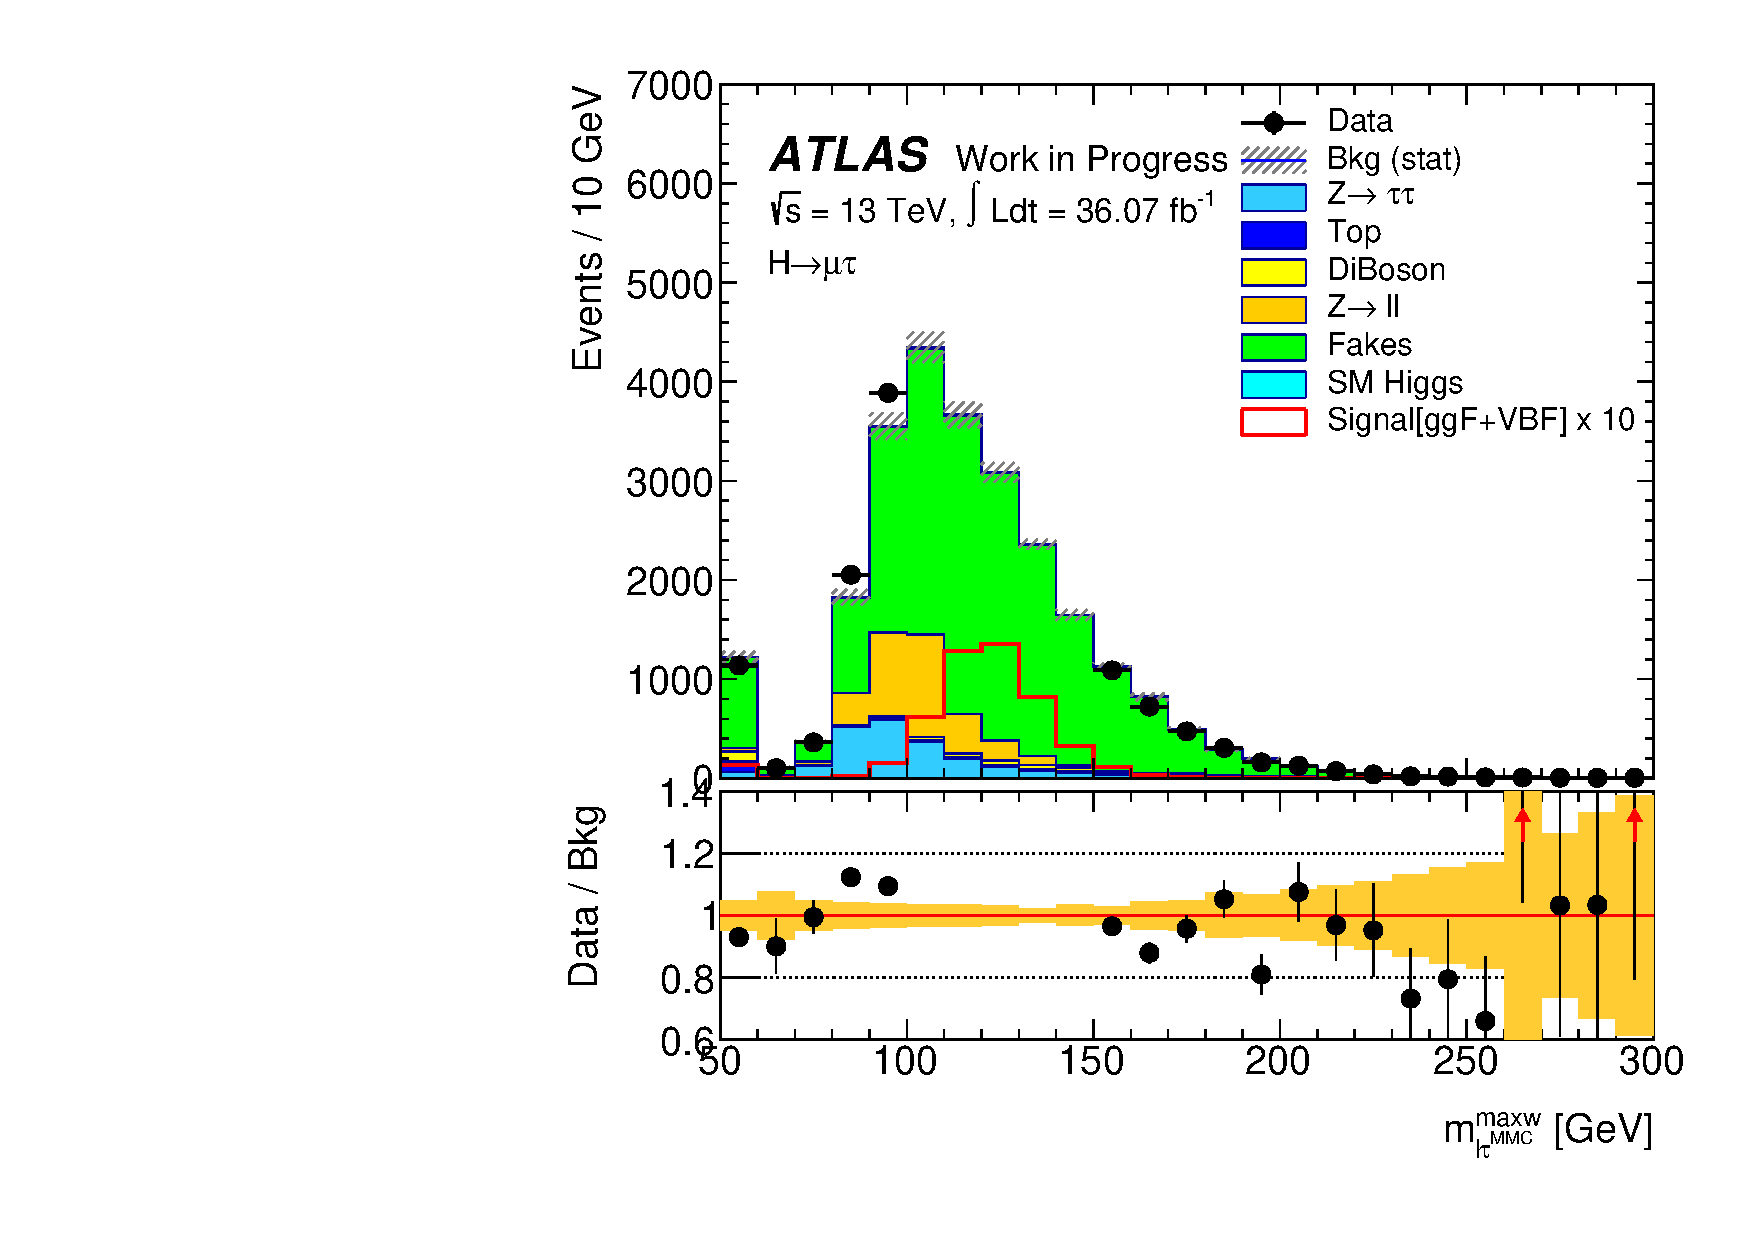
\includegraphics[width=.30\textwidth,height=.30\textheight,type=pdf,ext=.pdf,read=.pdf]{/afs/cern.ch/user/a/atpathak/afswork/public/Pixel/LFV_Plots/Plots_Qframework_25Apr2018_Final_note/plots_mcZll/mtau-CutTauPtSR3-MMCBL-lin}
\end{normalsize}
\end{frame}
%-----------------------------------------------
\begin{frame}
\frametitle{Distributions of $\mu\tau_{had}$ events in the SR1' region.}
\begin{normalsize}
\vspace*{0.2cm}
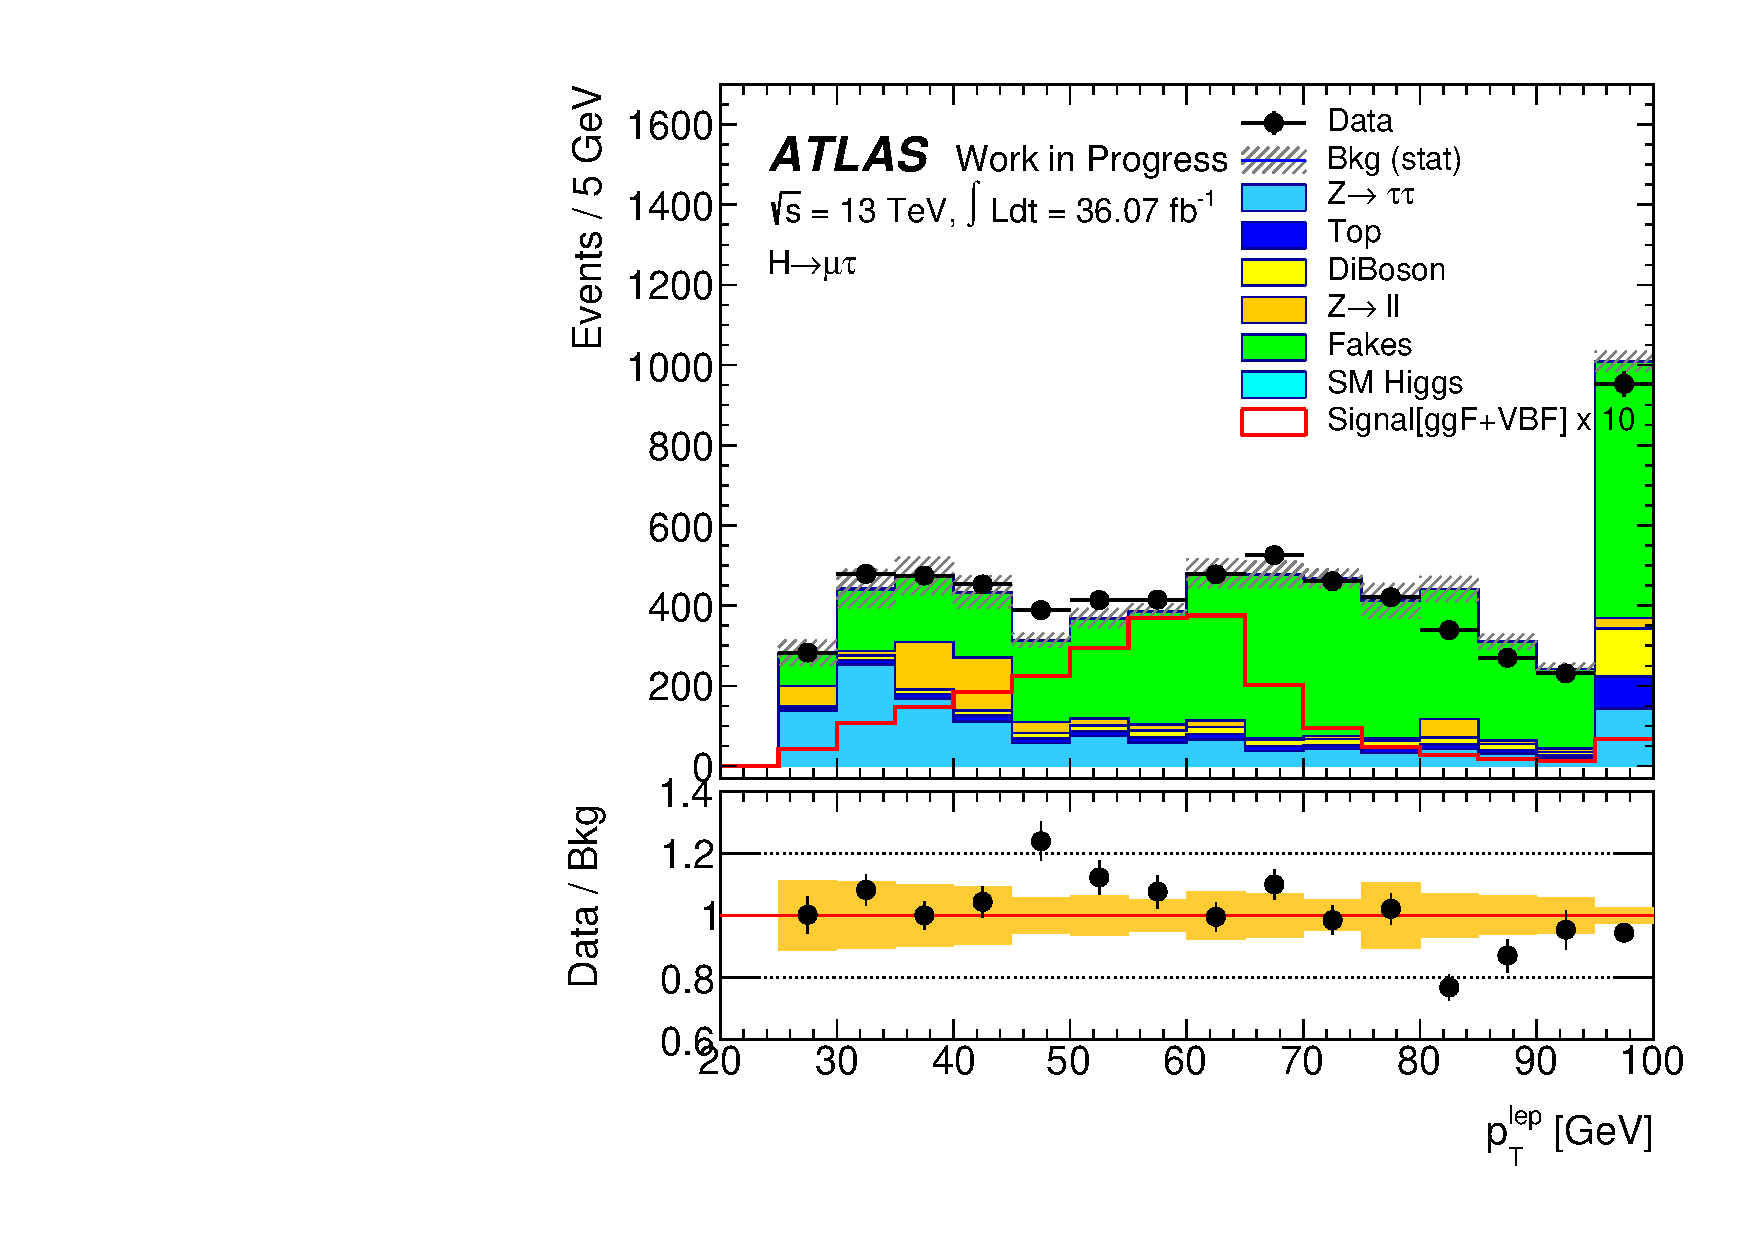
\includegraphics[width=.30\textwidth,height=.30\textheight,type=pdf,ext=.pdf,read=.pdf]{/afs/cern.ch/user/a/atpathak/afswork/public/Pixel/LFV_Plots/Plots_Qframework_25Apr2018_Final_note/plots_mcZll/mtau-CutTauMTSR1_VBF-leptonPt-lin}
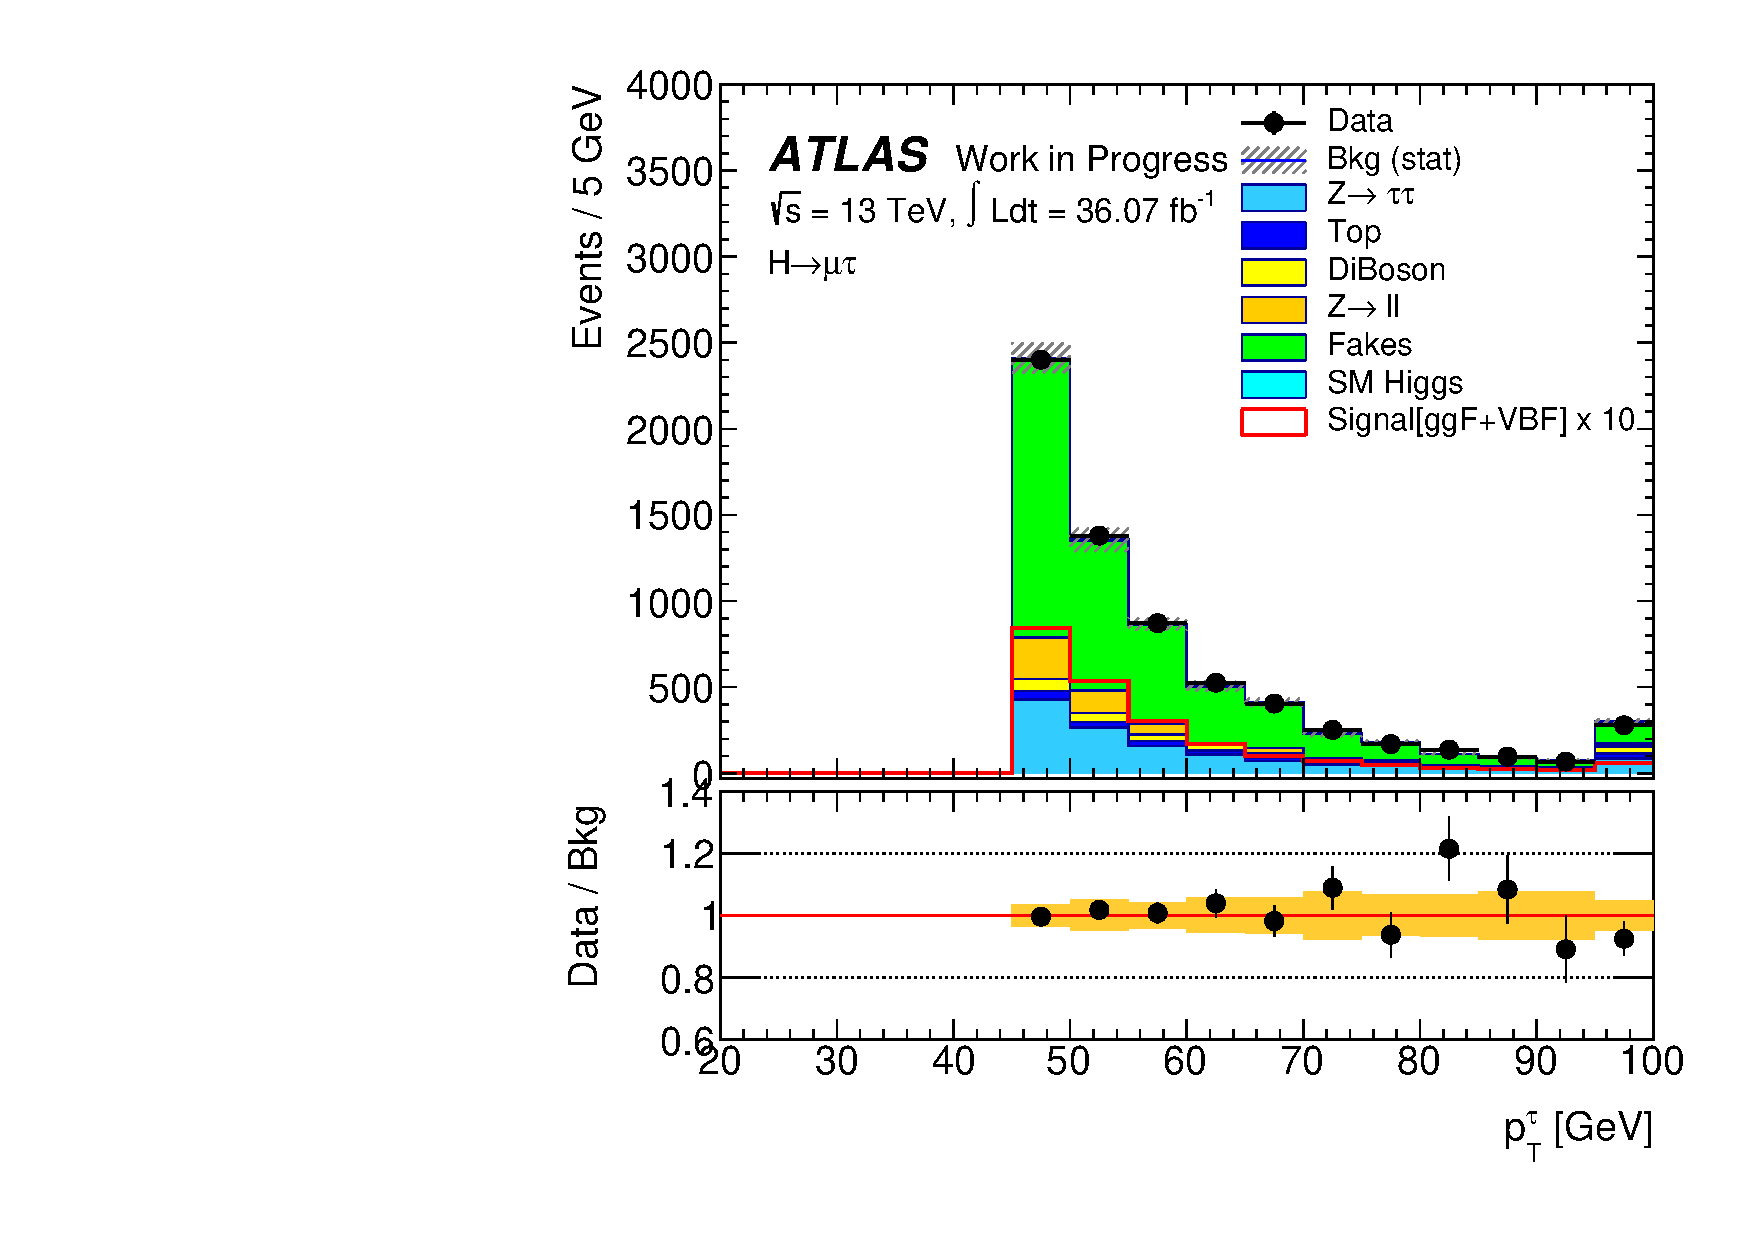
\includegraphics[width=.30\textwidth,height=.30\textheight,type=pdf,ext=.pdf,read=.pdf]{/afs/cern.ch/user/a/atpathak/afswork/public/Pixel/LFV_Plots/Plots_Qframework_25Apr2018_Final_note/plots_mcZll/mtau-CutTauMTSR1_VBF-tauPt-lin}
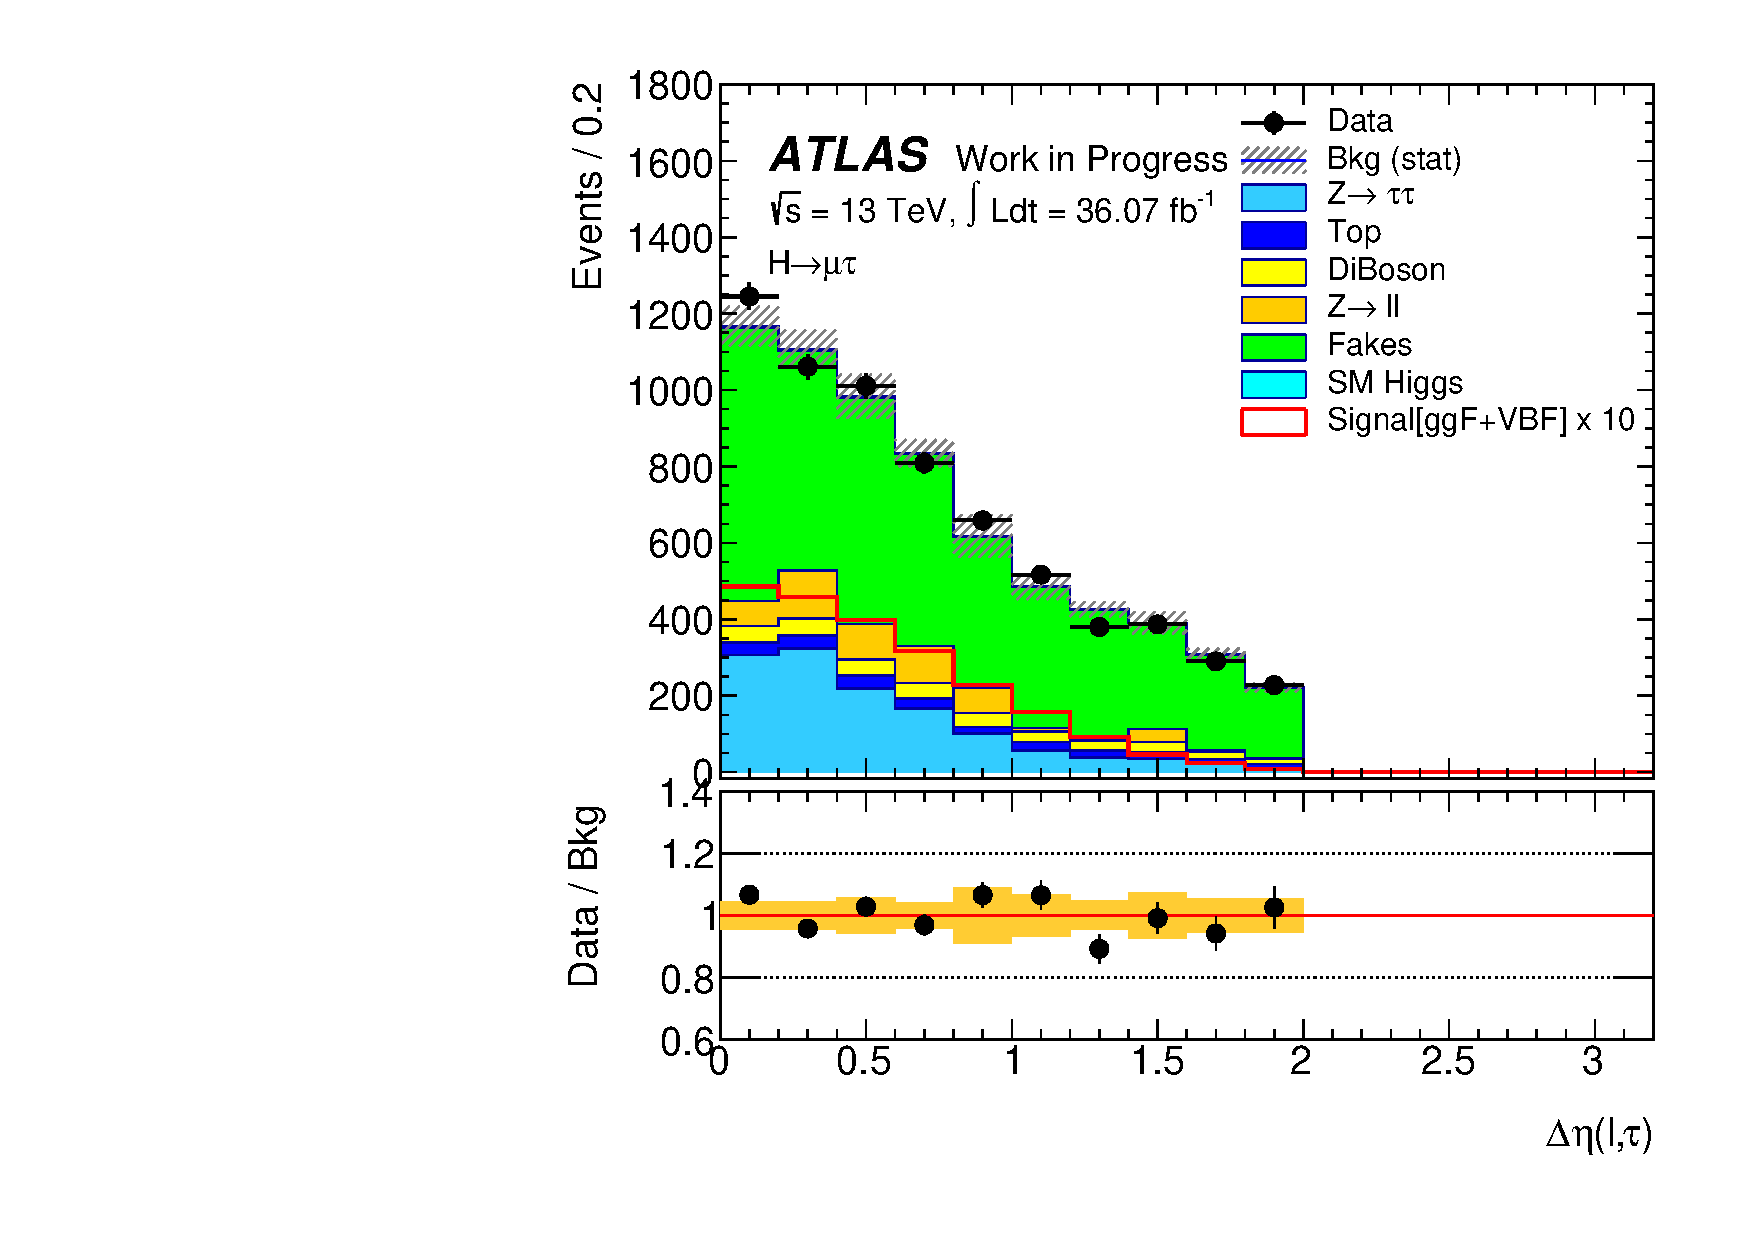
\includegraphics[width=.30\textwidth,height=.30\textheight,type=pdf,ext=.pdf,read=.pdf]{/afs/cern.ch/user/a/atpathak/afswork/public/Pixel/LFV_Plots/Plots_Qframework_25Apr2018_Final_note/plots_mcZll/mtau-CutTauMTSR1_VBF-dEtaTauLep-lin}\\
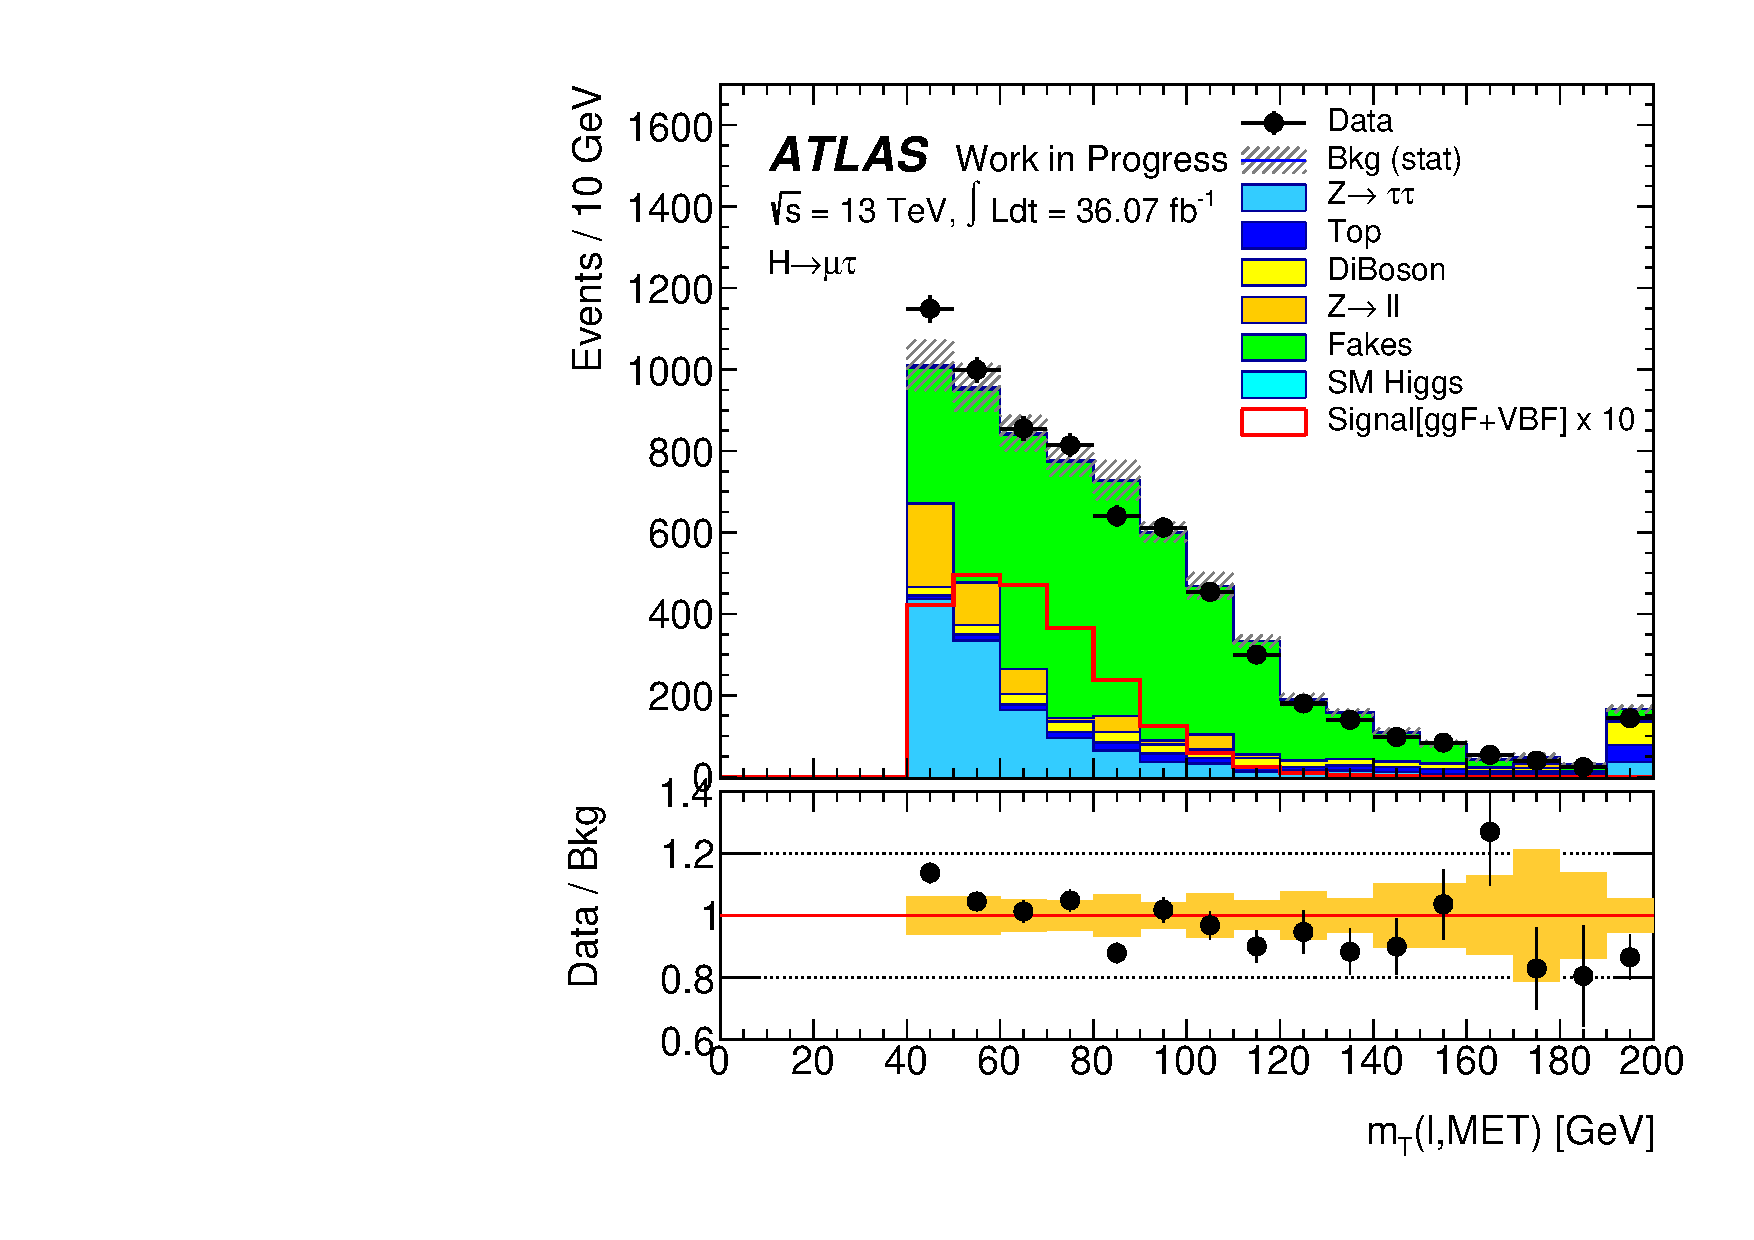
\includegraphics[width=.30\textwidth,height=.30\textheight,type=pdf,ext=.pdf,read=.pdf]{/afs/cern.ch/user/a/atpathak/afswork/public/Pixel/LFV_Plots/Plots_Qframework_25Apr2018_Final_note/plots_mcZll/mtau-CutTauMTSR1_VBF-transverseMassLepMET-lin}
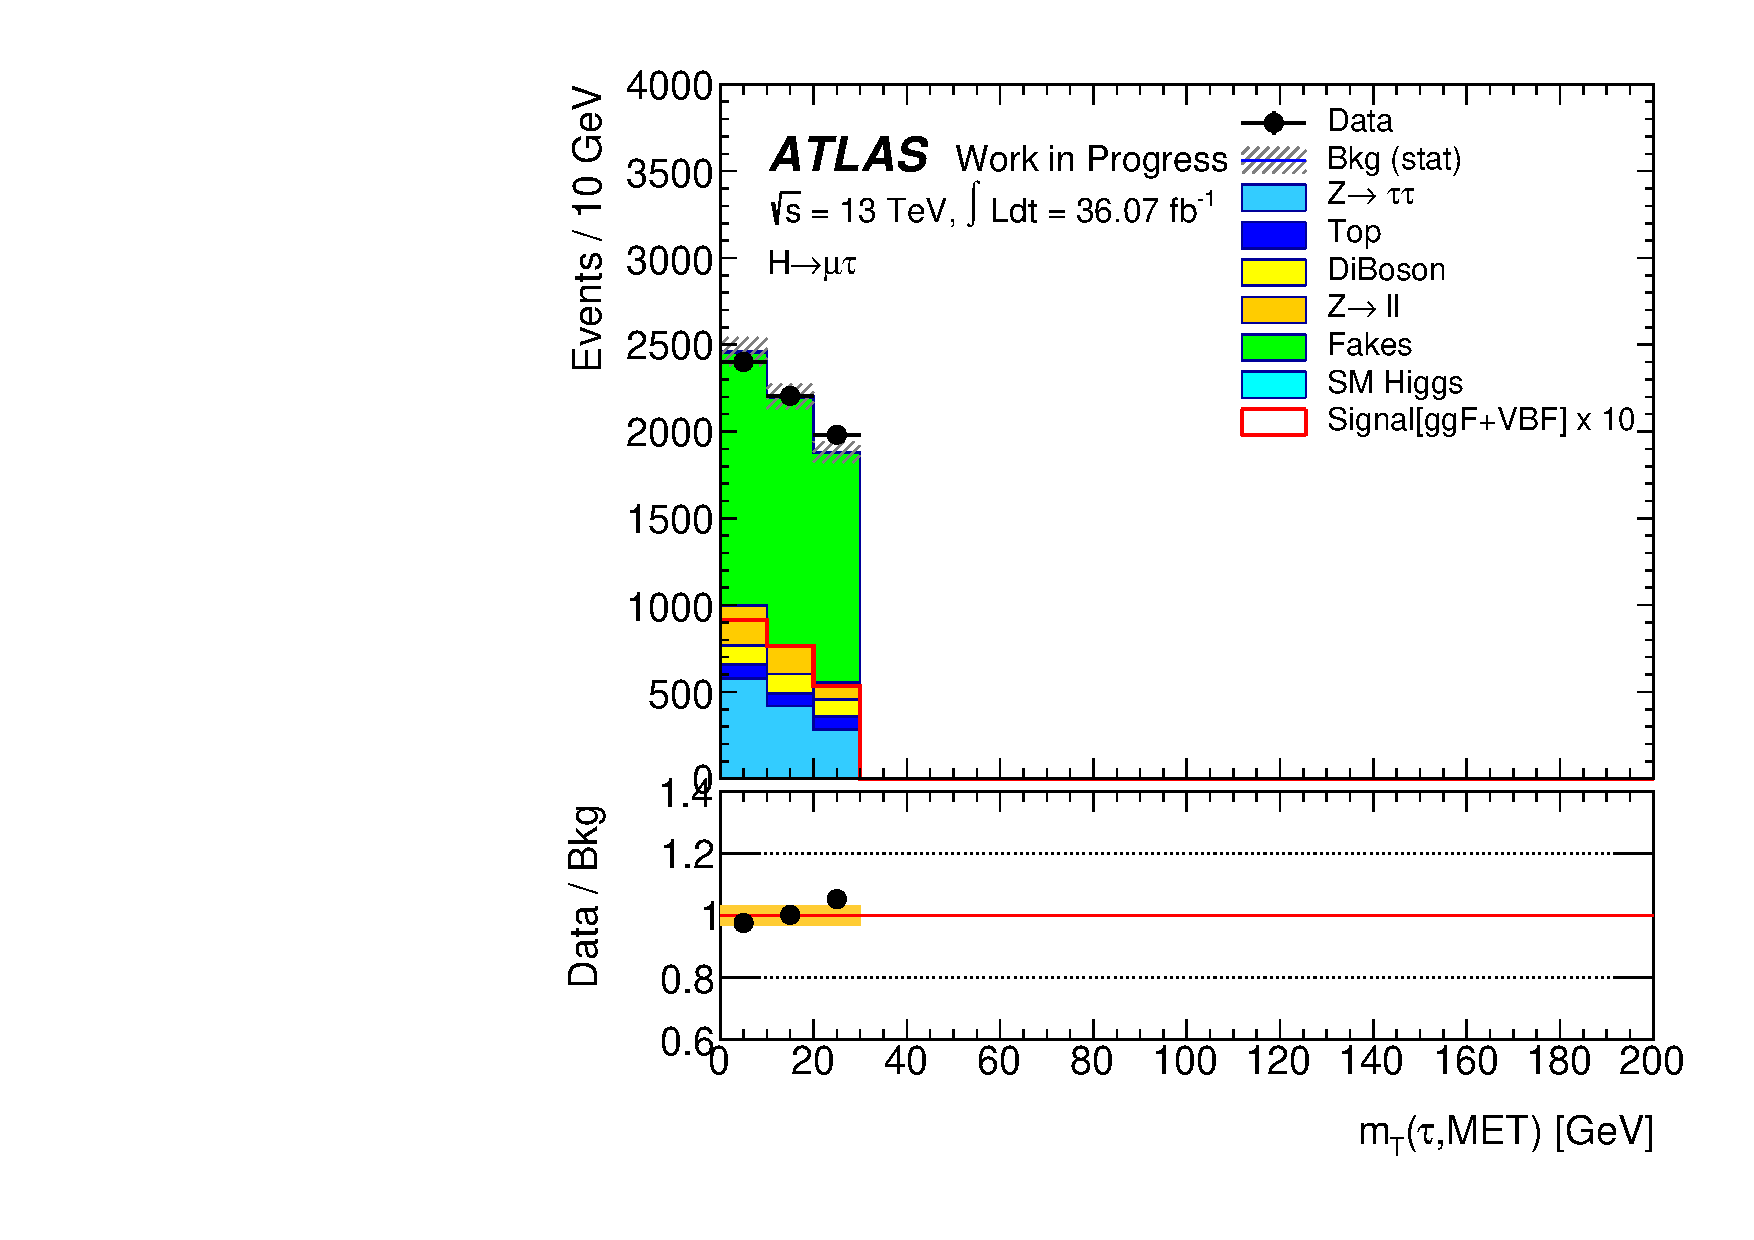
\includegraphics[width=.30\textwidth,height=.30\textheight,type=pdf,ext=.pdf,read=.pdf]{/afs/cern.ch/user/a/atpathak/afswork/public/Pixel/LFV_Plots/Plots_Qframework_25Apr2018_Final_note/plots_mcZll/mtau-CutTauMTSR1_VBF-transverseMassTauMET-lin}
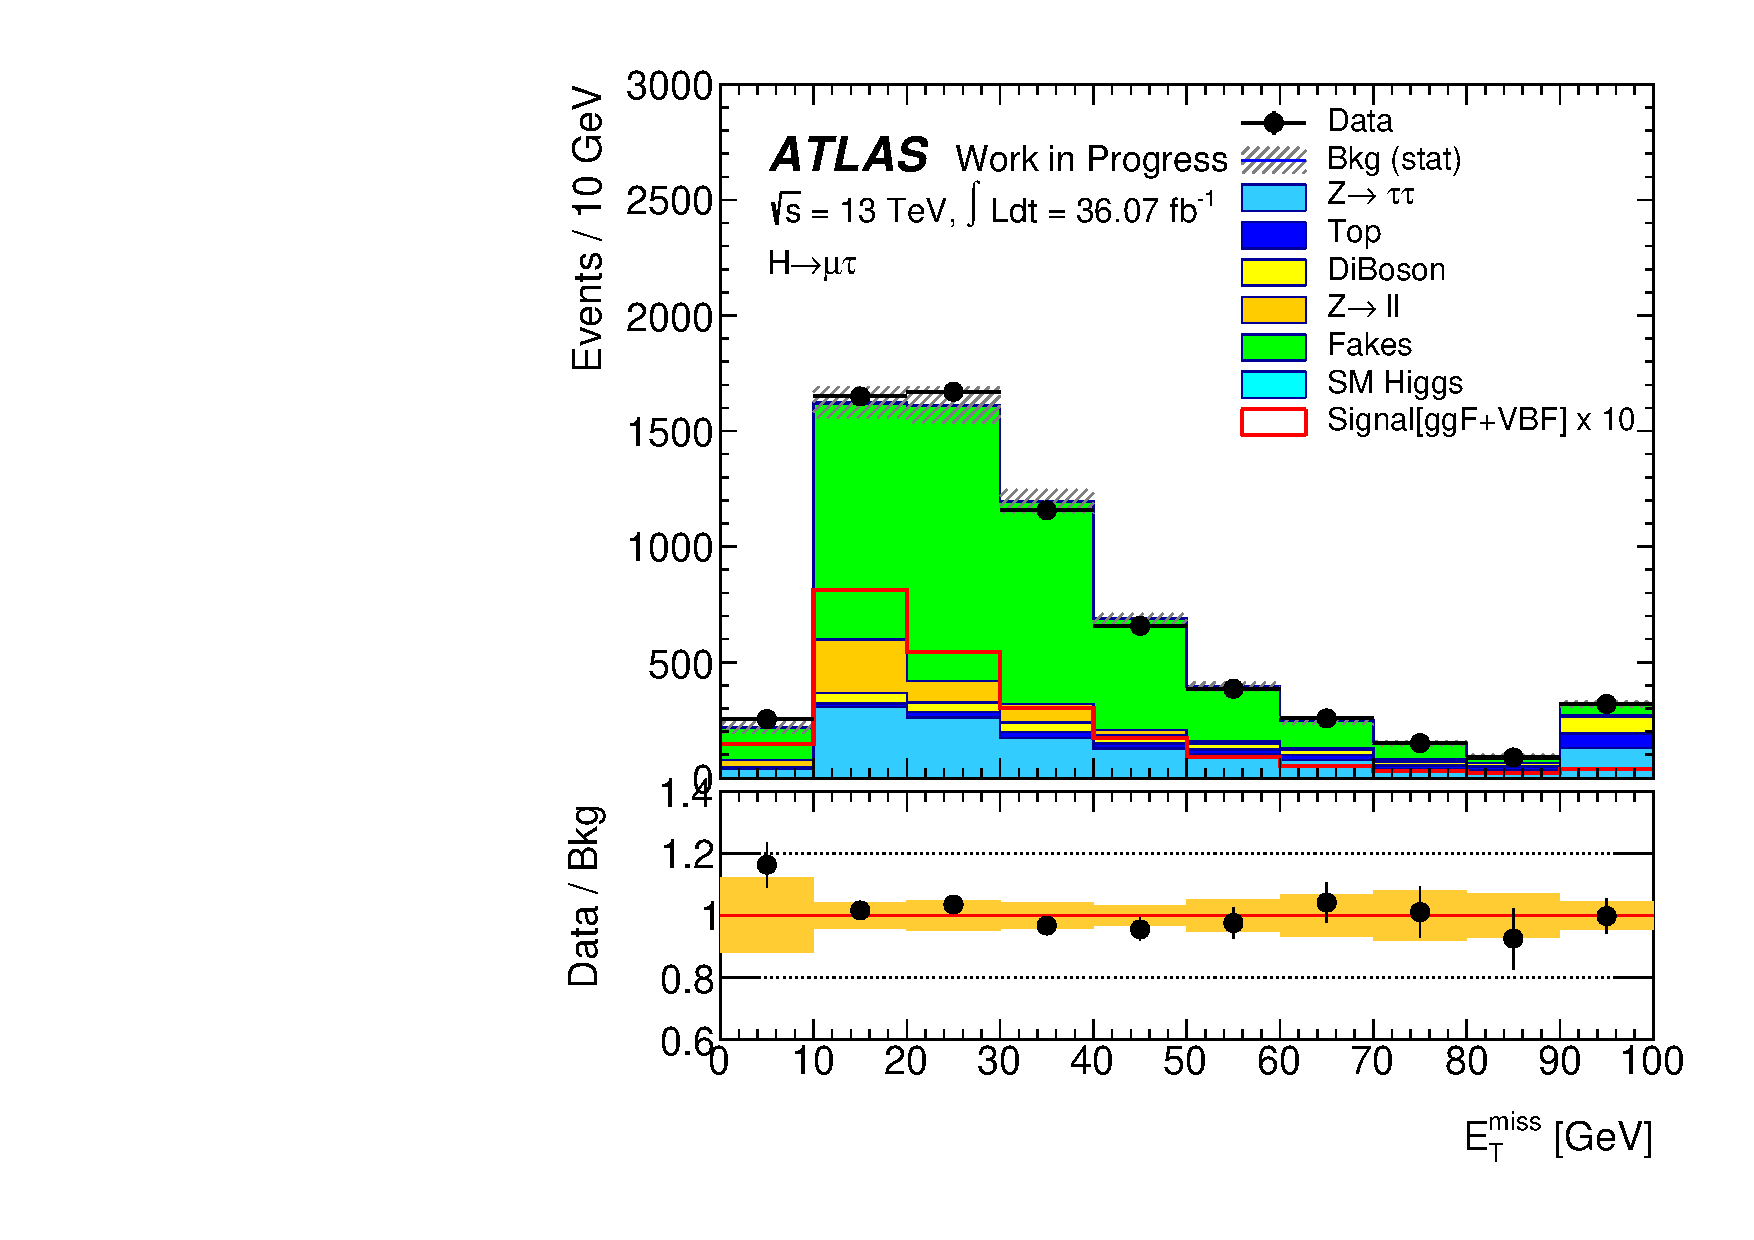
\includegraphics[width=.30\textwidth,height=.30\textheight,type=pdf,ext=.pdf,read=.pdf]{/afs/cern.ch/user/a/atpathak/afswork/public/Pixel/LFV_Plots/Plots_Qframework_25Apr2018_Final_note/plots_mcZll/mtau-CutTauMTSR1_VBF-met-lin}\\
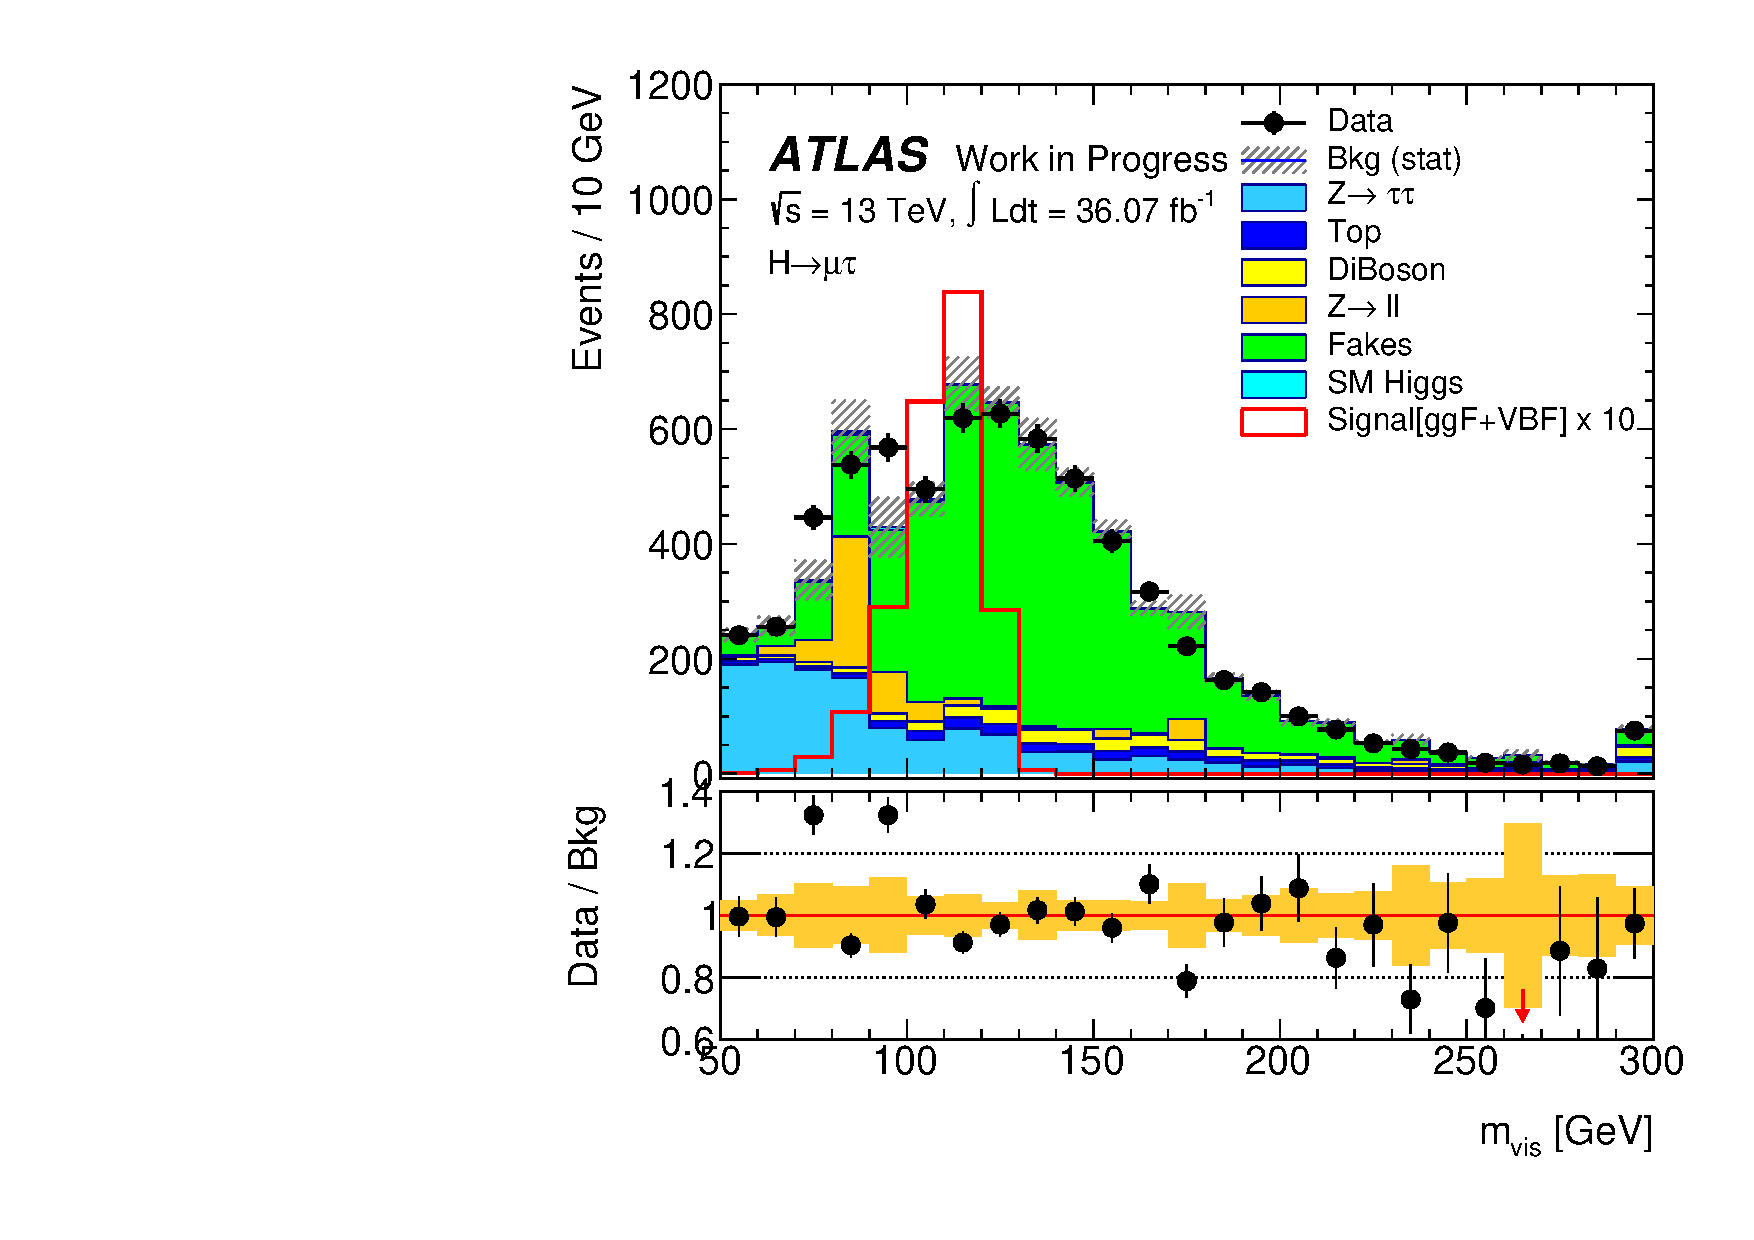
\includegraphics[width=.30\textwidth,height=.30\textheight,type=pdf,ext=.pdf,read=.pdf]{/afs/cern.ch/user/a/atpathak/afswork/public/Pixel/LFV_Plots/Plots_Qframework_25Apr2018_Final_note/plots_mcZll/mtau-CutTauMTSR1_VBF-visibleMass-lin}
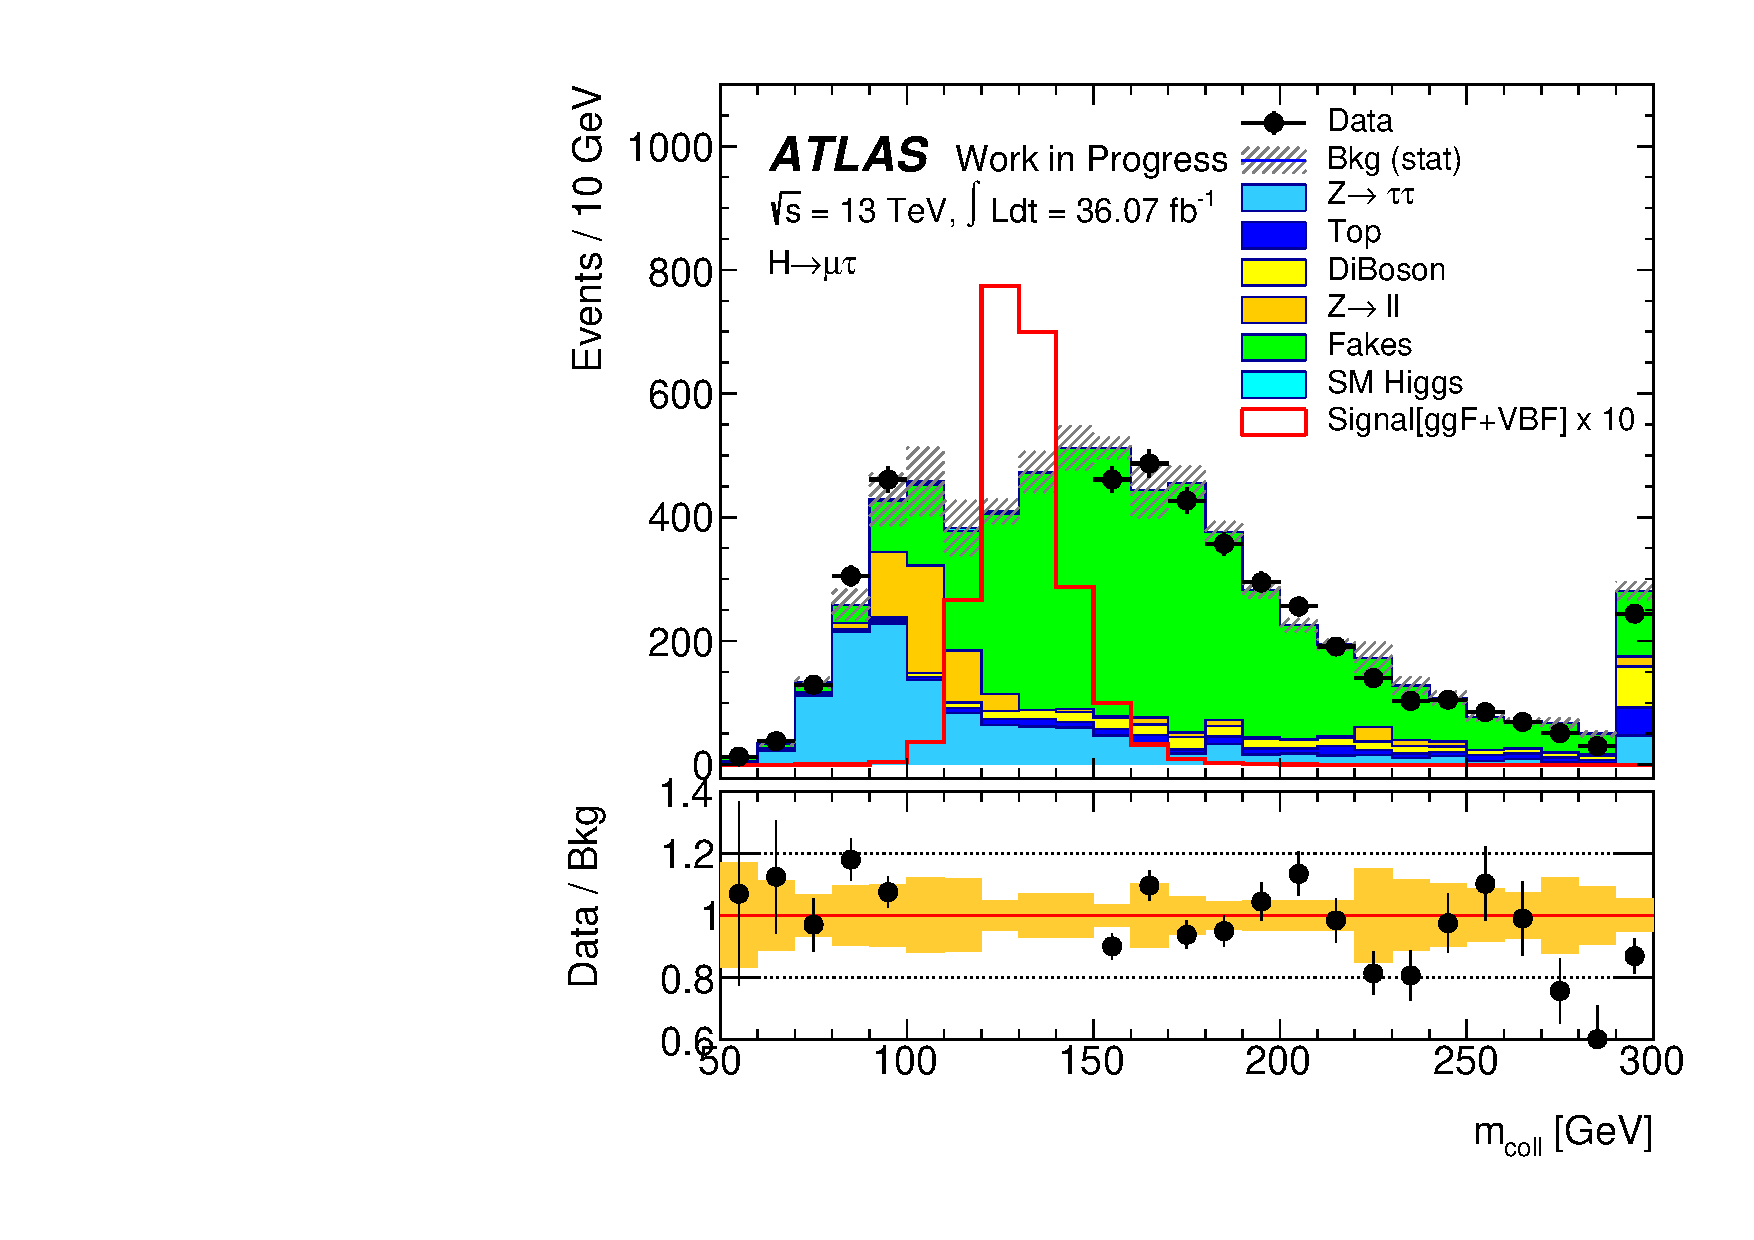
\includegraphics[width=.30\textwidth,height=.30\textheight,type=pdf,ext=.pdf,read=.pdf]{/afs/cern.ch/user/a/atpathak/afswork/public/Pixel/LFV_Plots/Plots_Qframework_25Apr2018_Final_note/plots_mcZll/mtau-CutTauMTSR1_VBF-collMassBL-lin}
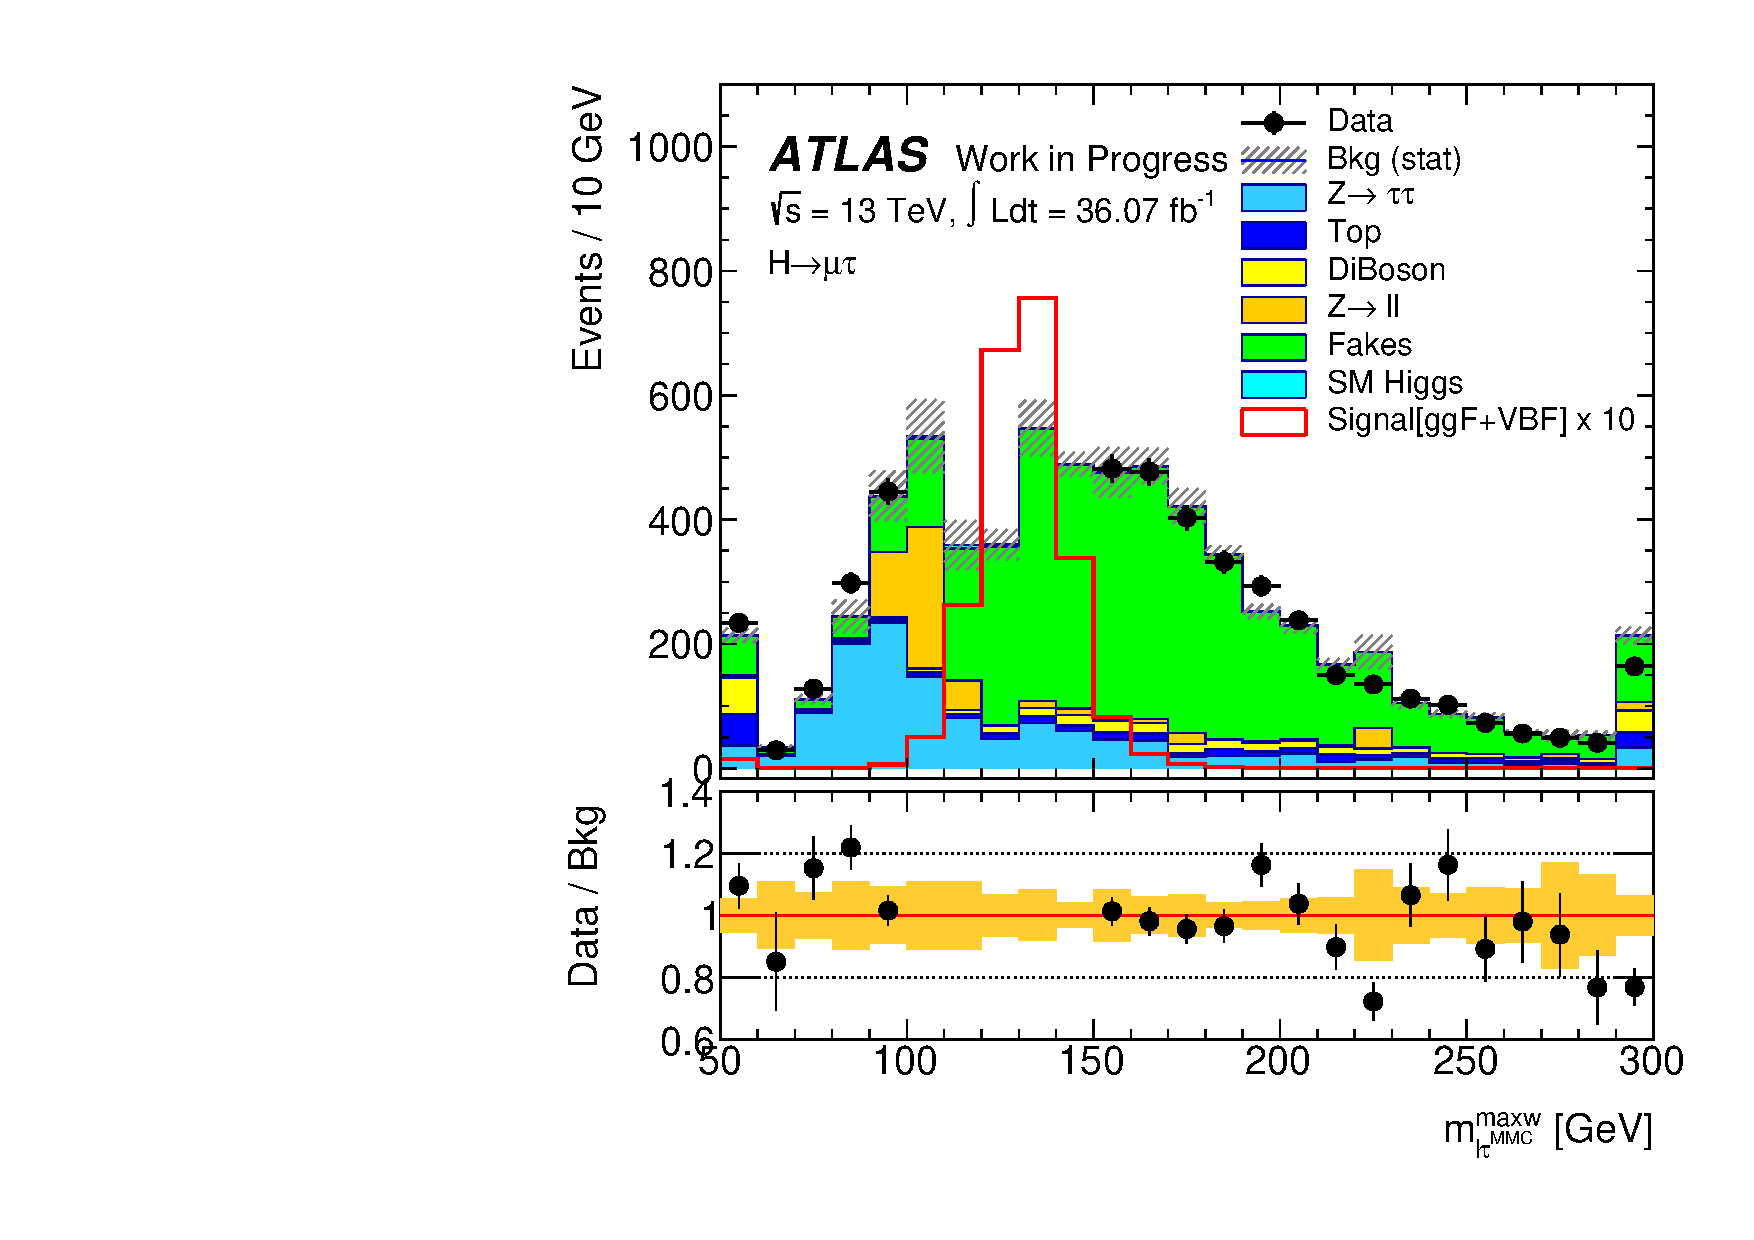
\includegraphics[width=.30\textwidth,height=.30\textheight,type=pdf,ext=.pdf,read=.pdf]{/afs/cern.ch/user/a/atpathak/afswork/public/Pixel/LFV_Plots/Plots_Qframework_25Apr2018_Final_note/plots_mcZll/mtau-CutTauMTSR1_VBF-MMCBL-lin}
\end{normalsize}
\end{frame}
%-----------------------------------------------
\begin{frame}
\frametitle{Distributions of $\mu\tau_{had}$ events in the SR2' region.}
\begin{normalsize}
\vspace*{0.2cm}
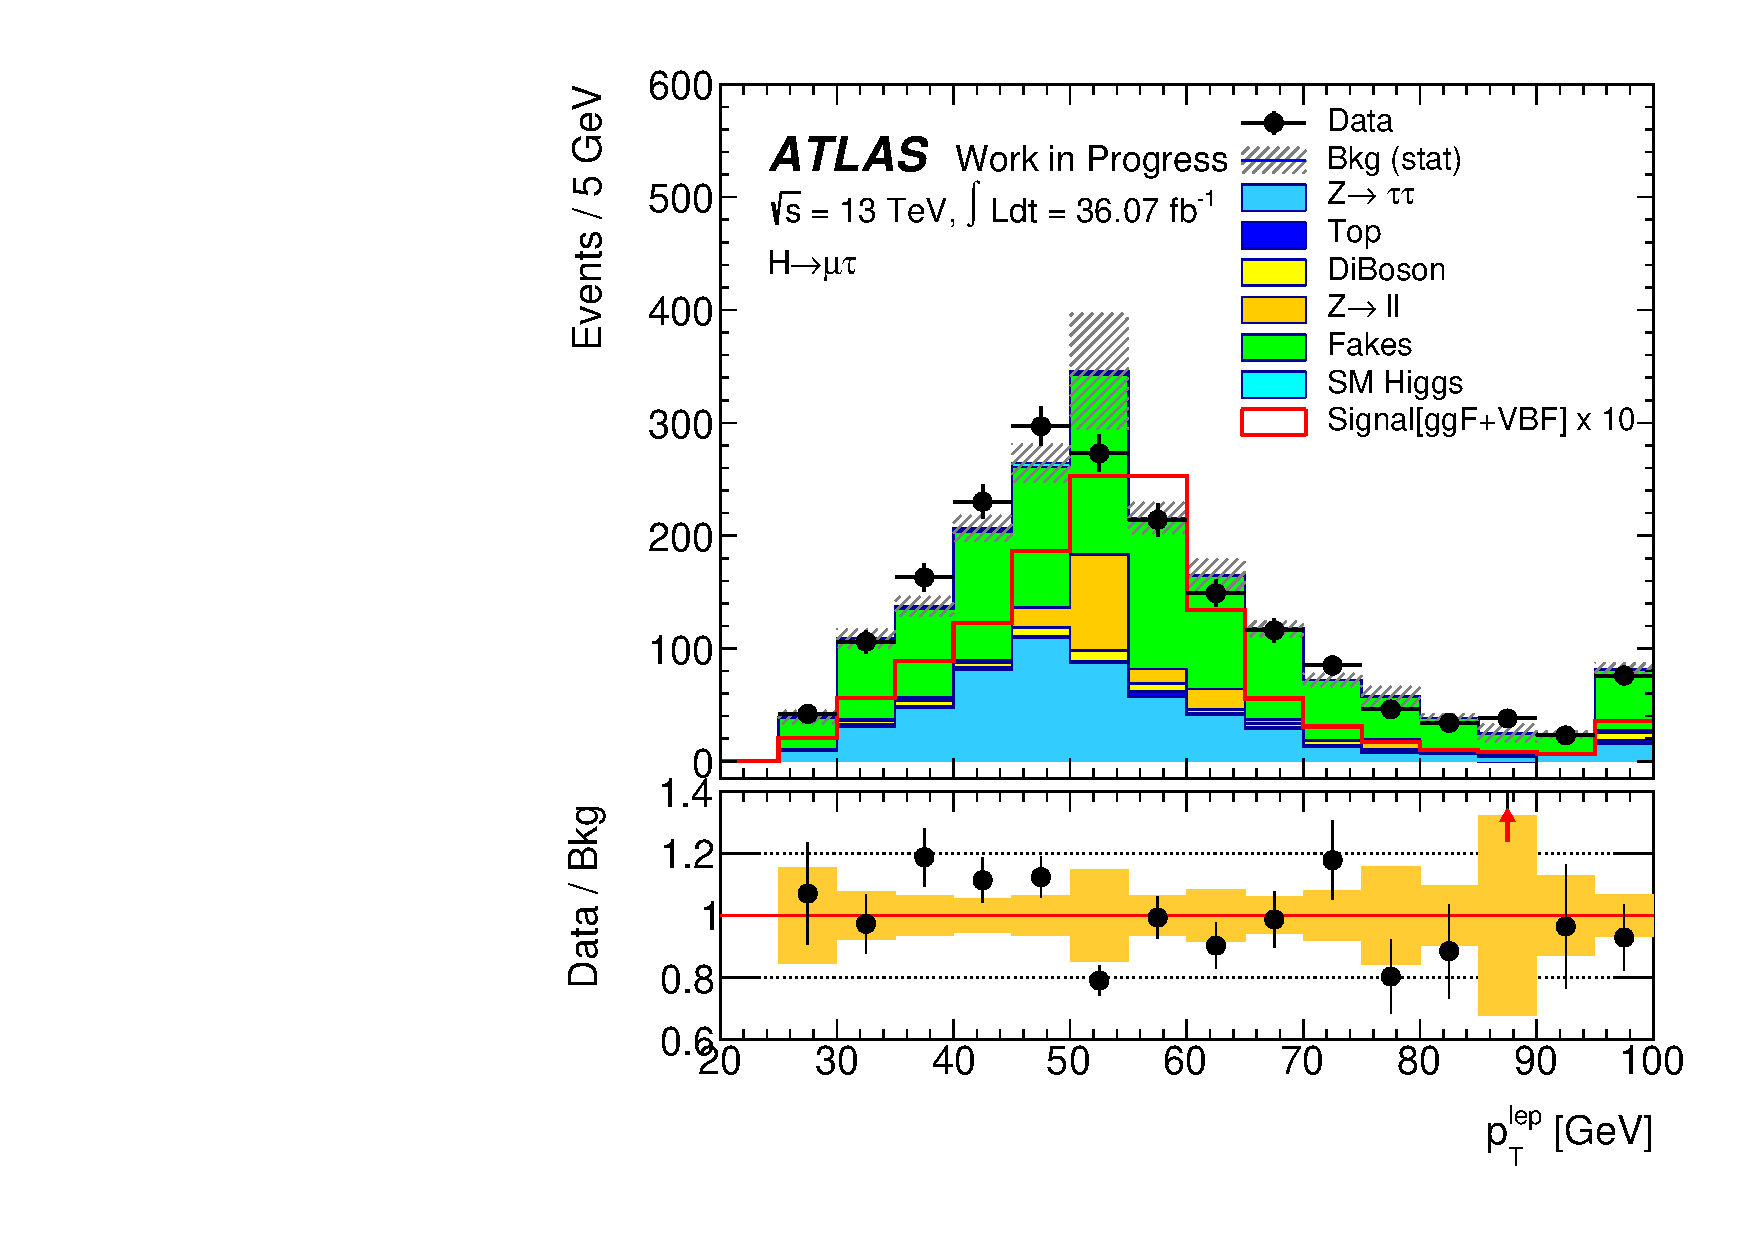
\includegraphics[width=.30\textwidth,height=.30\textheight,type=pdf,ext=.pdf,read=.pdf]{/afs/cern.ch/user/a/atpathak/afswork/public/Pixel/LFV_Plots/Plots_Qframework_25Apr2018_Final_note/plots_mcZll/mtau-CutTauMTSR2_VBF-leptonPt-lin}
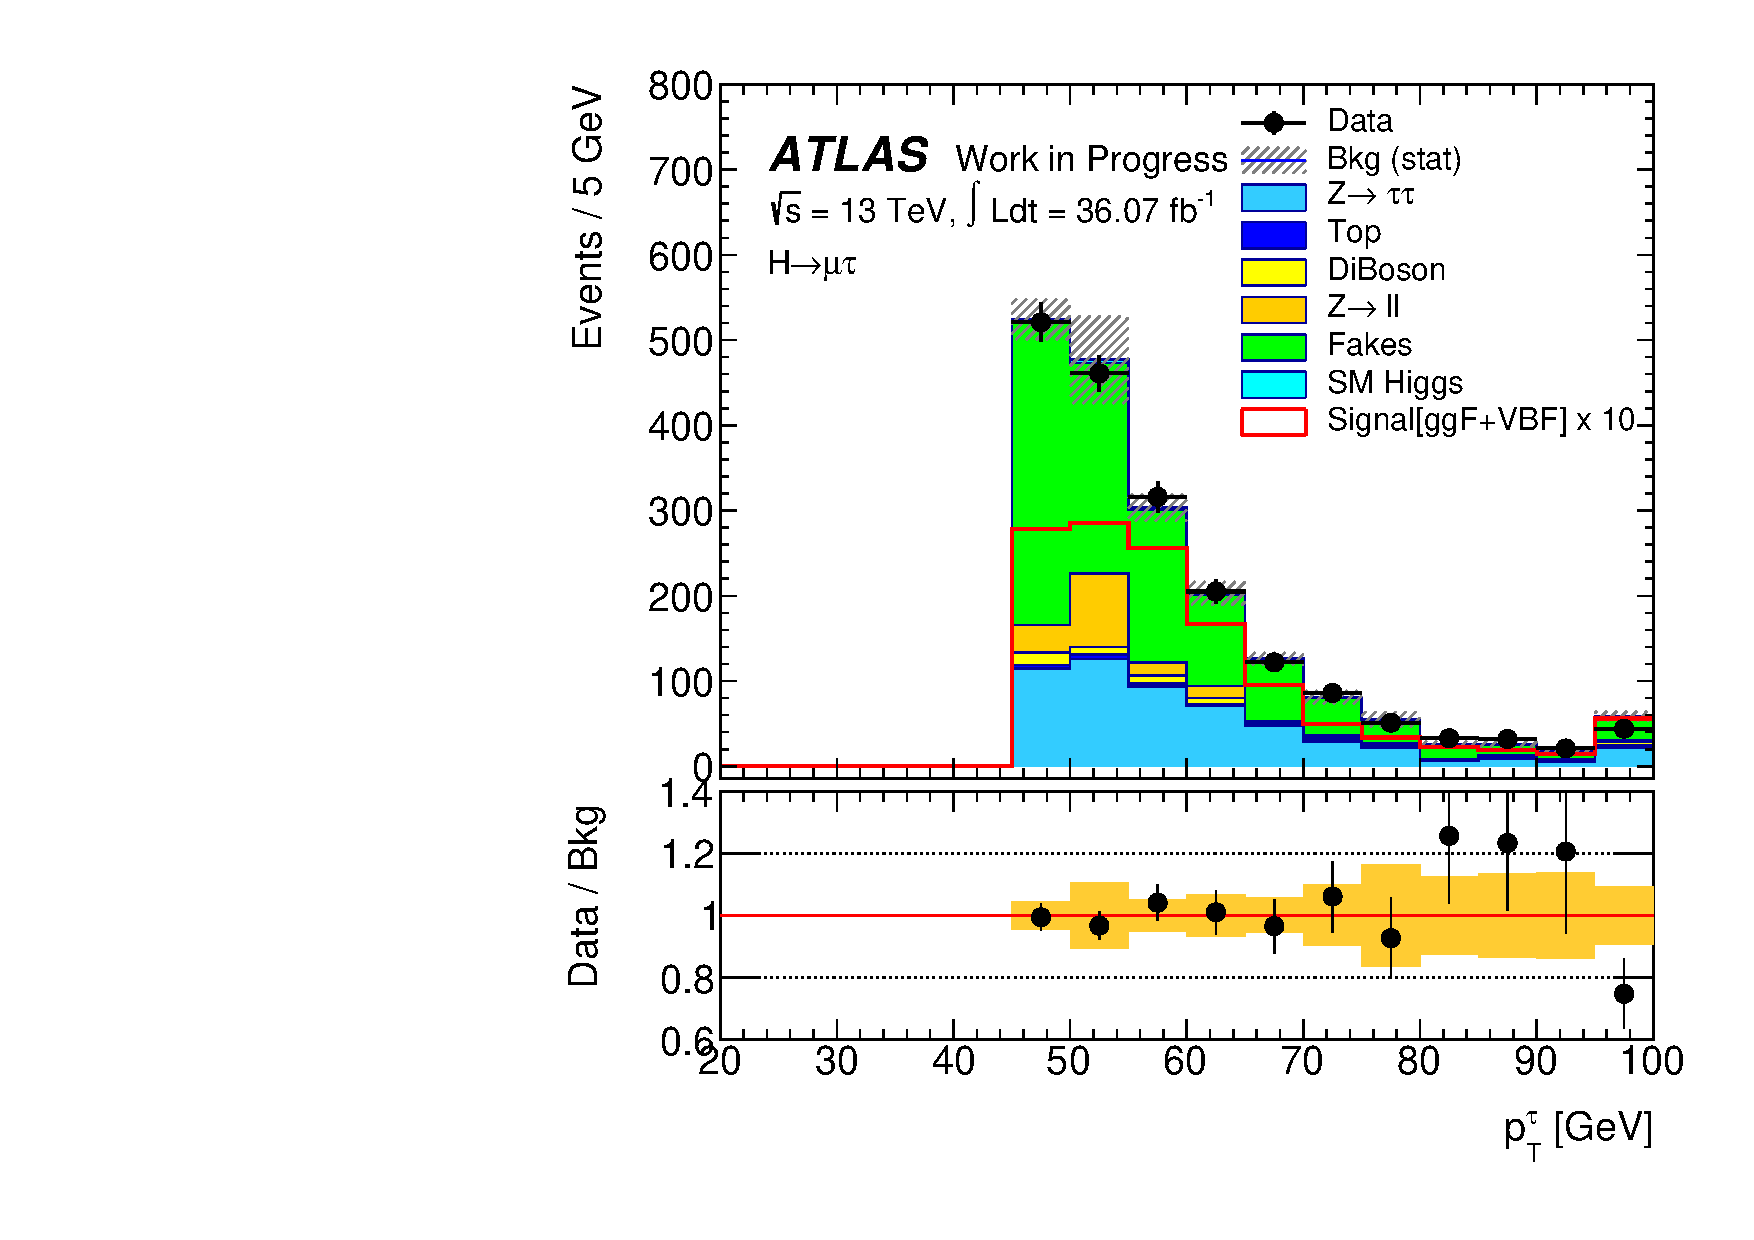
\includegraphics[width=.30\textwidth,height=.30\textheight,type=pdf,ext=.pdf,read=.pdf]{/afs/cern.ch/user/a/atpathak/afswork/public/Pixel/LFV_Plots/Plots_Qframework_25Apr2018_Final_note/plots_mcZll/mtau-CutTauMTSR2_VBF-tauPt-lin}
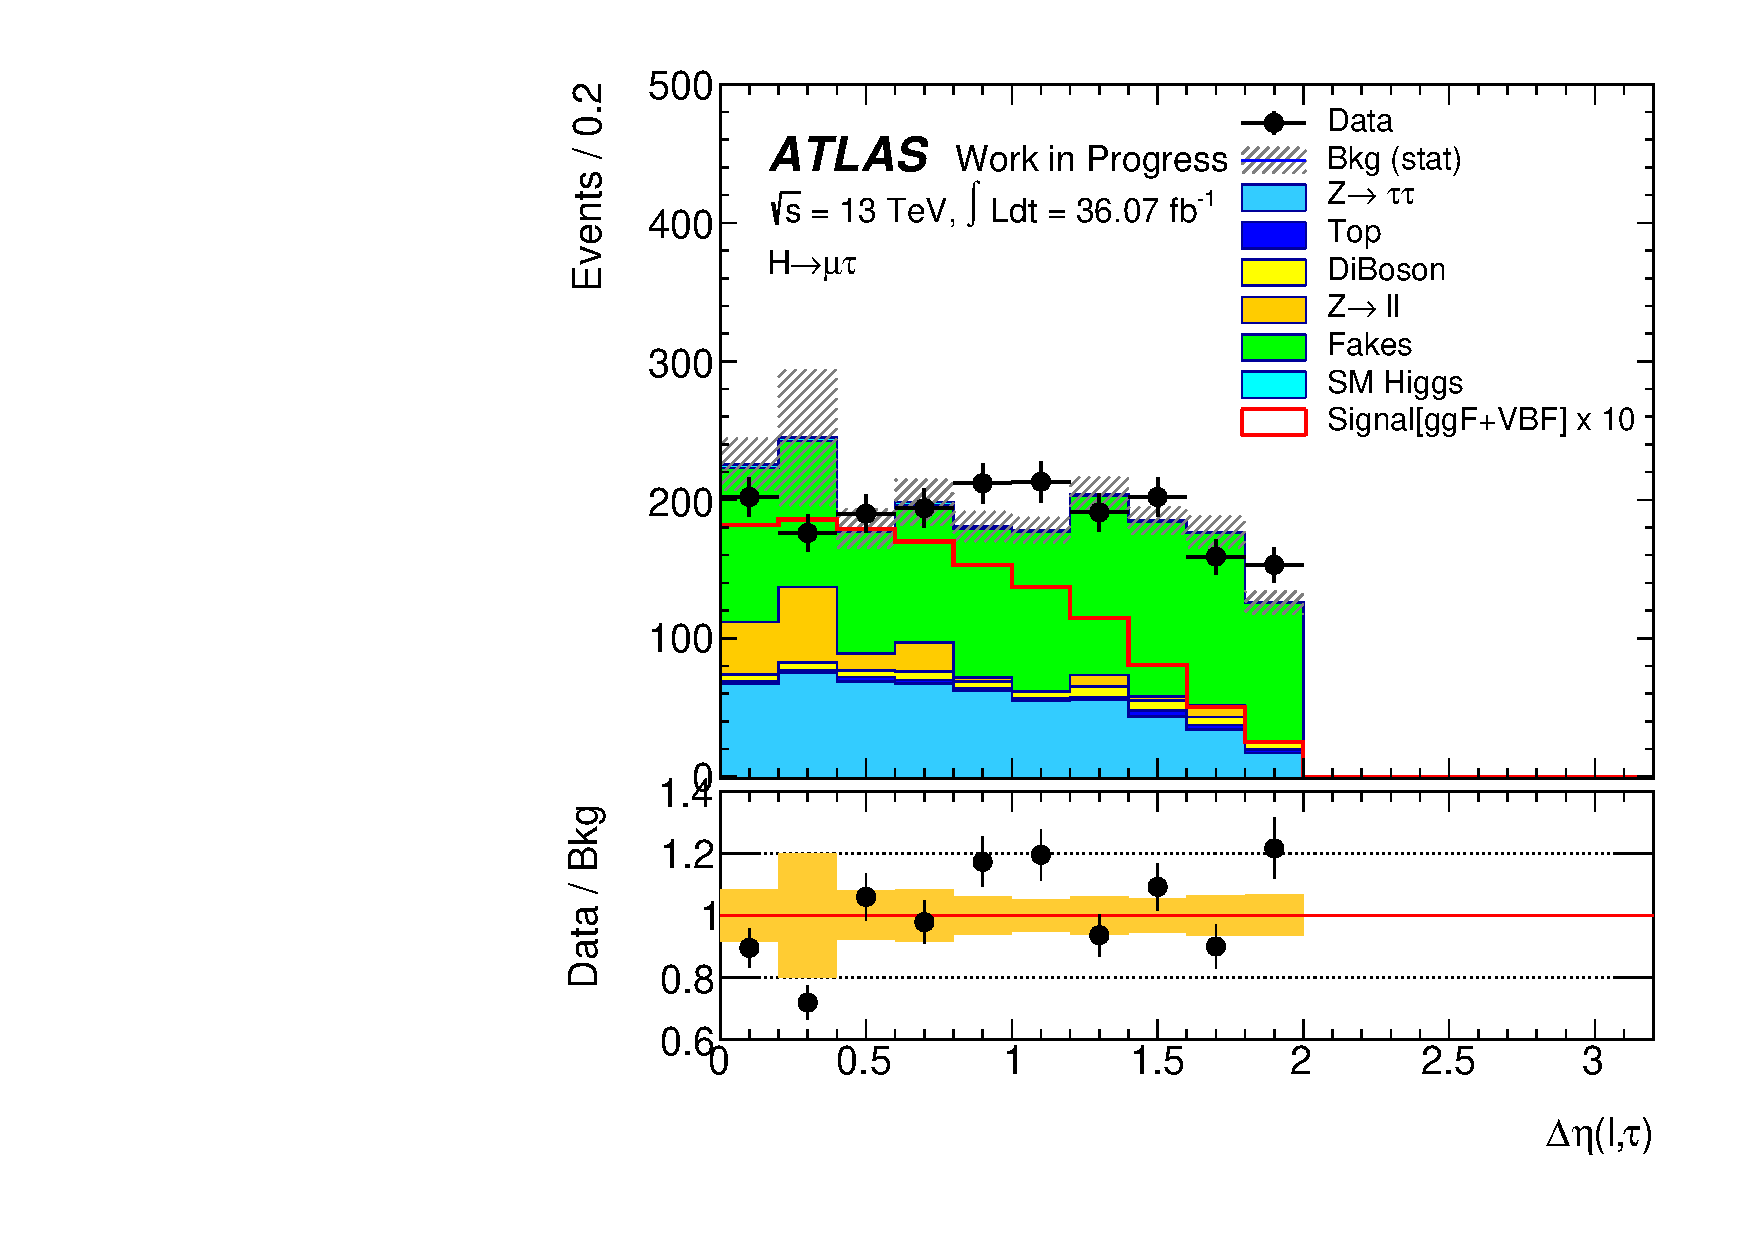
\includegraphics[width=.30\textwidth,height=.30\textheight,type=pdf,ext=.pdf,read=.pdf]{/afs/cern.ch/user/a/atpathak/afswork/public/Pixel/LFV_Plots/Plots_Qframework_25Apr2018_Final_note/plots_mcZll/mtau-CutTauMTSR2_VBF-dEtaTauLep-lin}\\
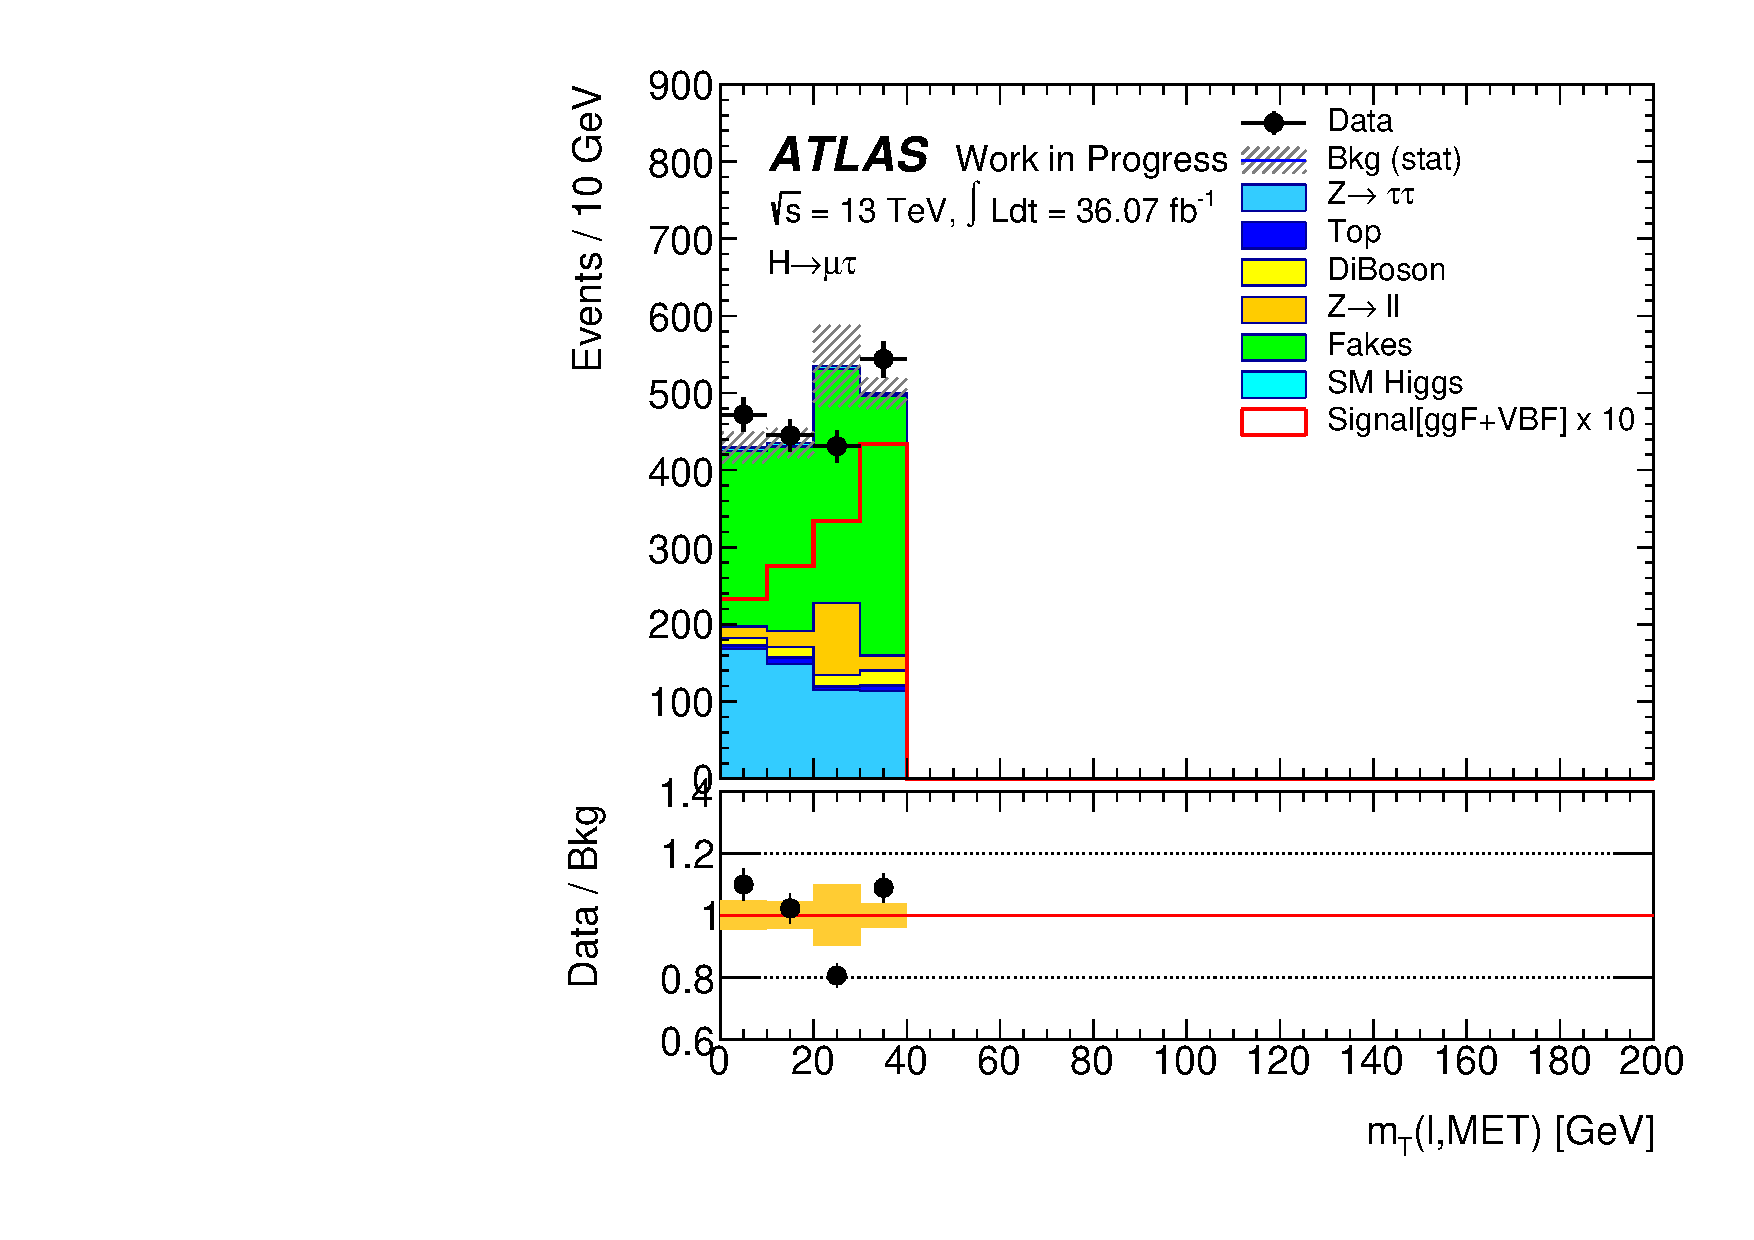
\includegraphics[width=.30\textwidth,height=.30\textheight,type=pdf,ext=.pdf,read=.pdf]{/afs/cern.ch/user/a/atpathak/afswork/public/Pixel/LFV_Plots/Plots_Qframework_25Apr2018_Final_note/plots_mcZll/mtau-CutTauMTSR2_VBF-transverseMassLepMET-lin}
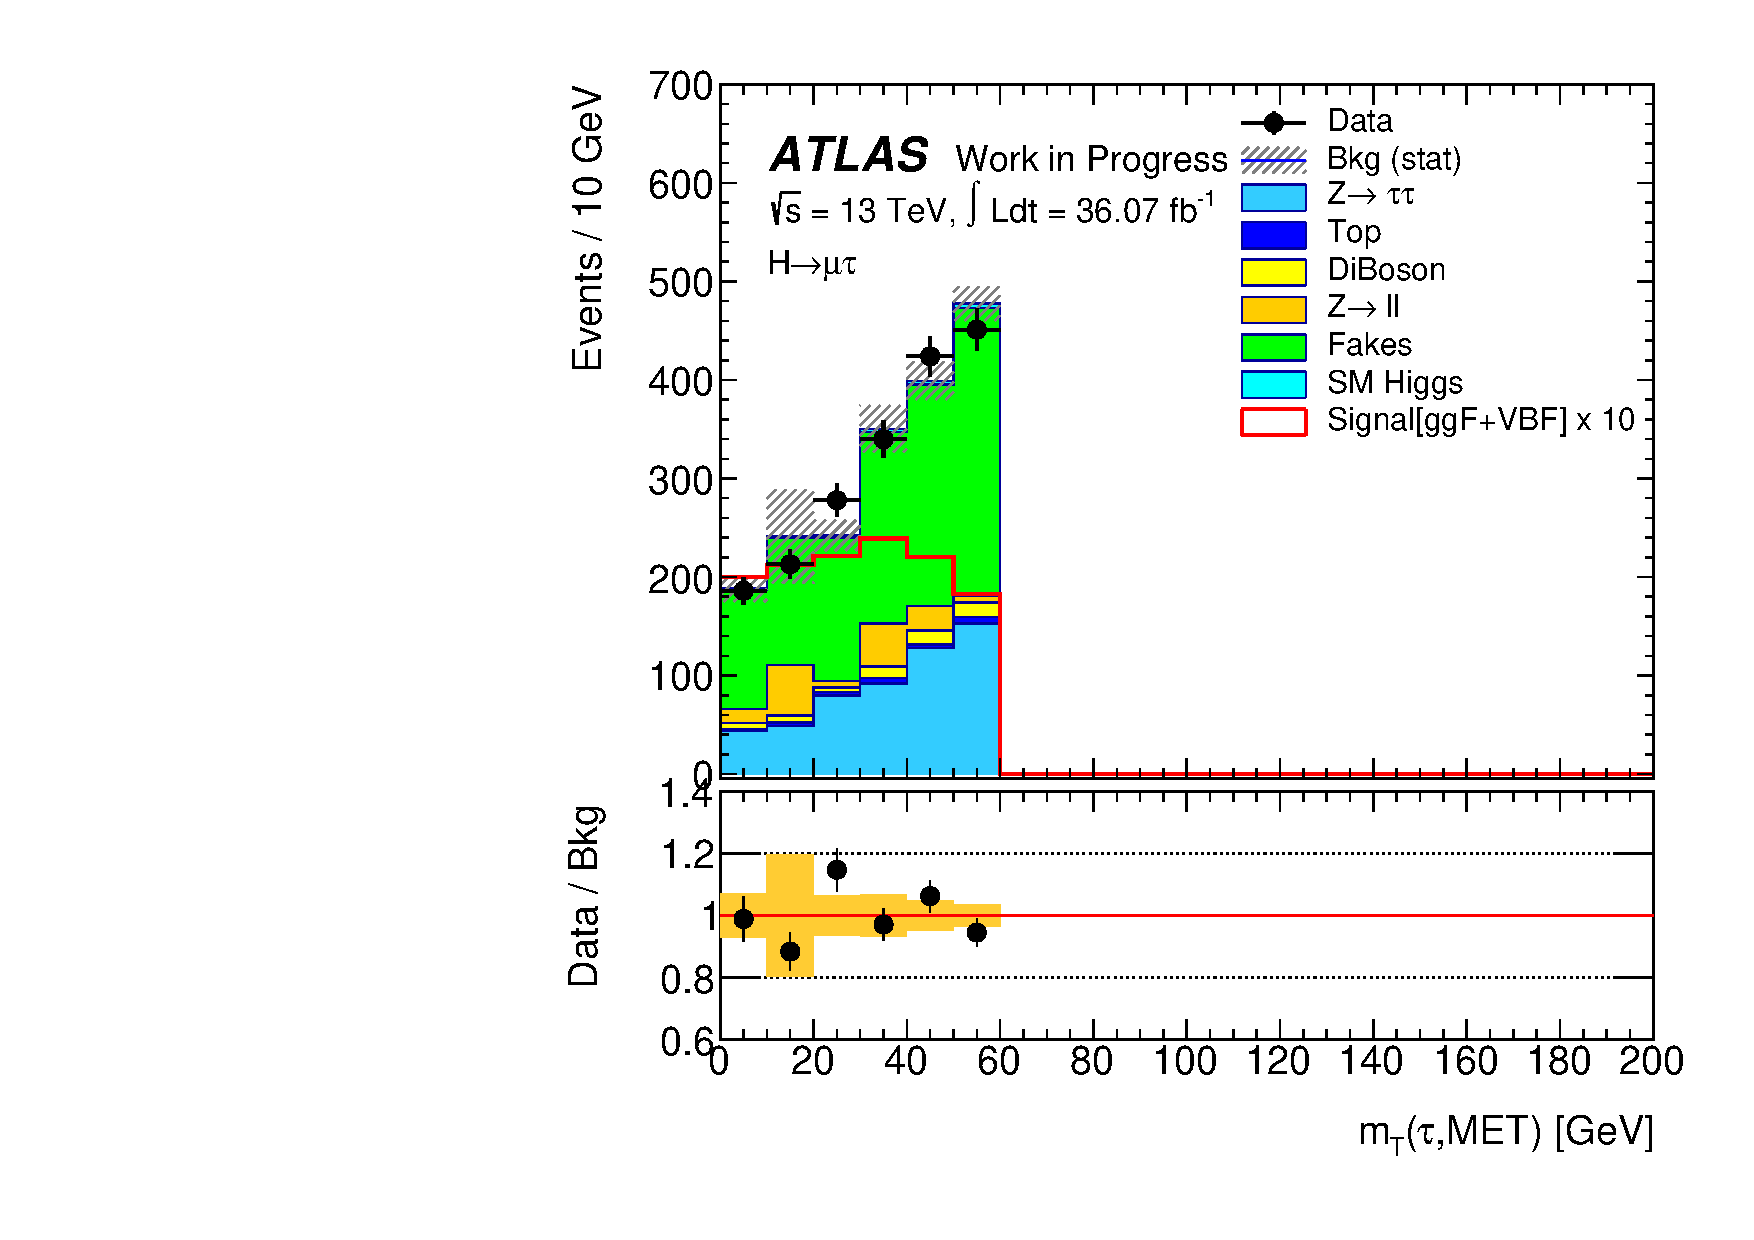
\includegraphics[width=.30\textwidth,height=.30\textheight,type=pdf,ext=.pdf,read=.pdf]{/afs/cern.ch/user/a/atpathak/afswork/public/Pixel/LFV_Plots/Plots_Qframework_25Apr2018_Final_note/plots_mcZll/mtau-CutTauMTSR2_VBF-transverseMassTauMET-lin}
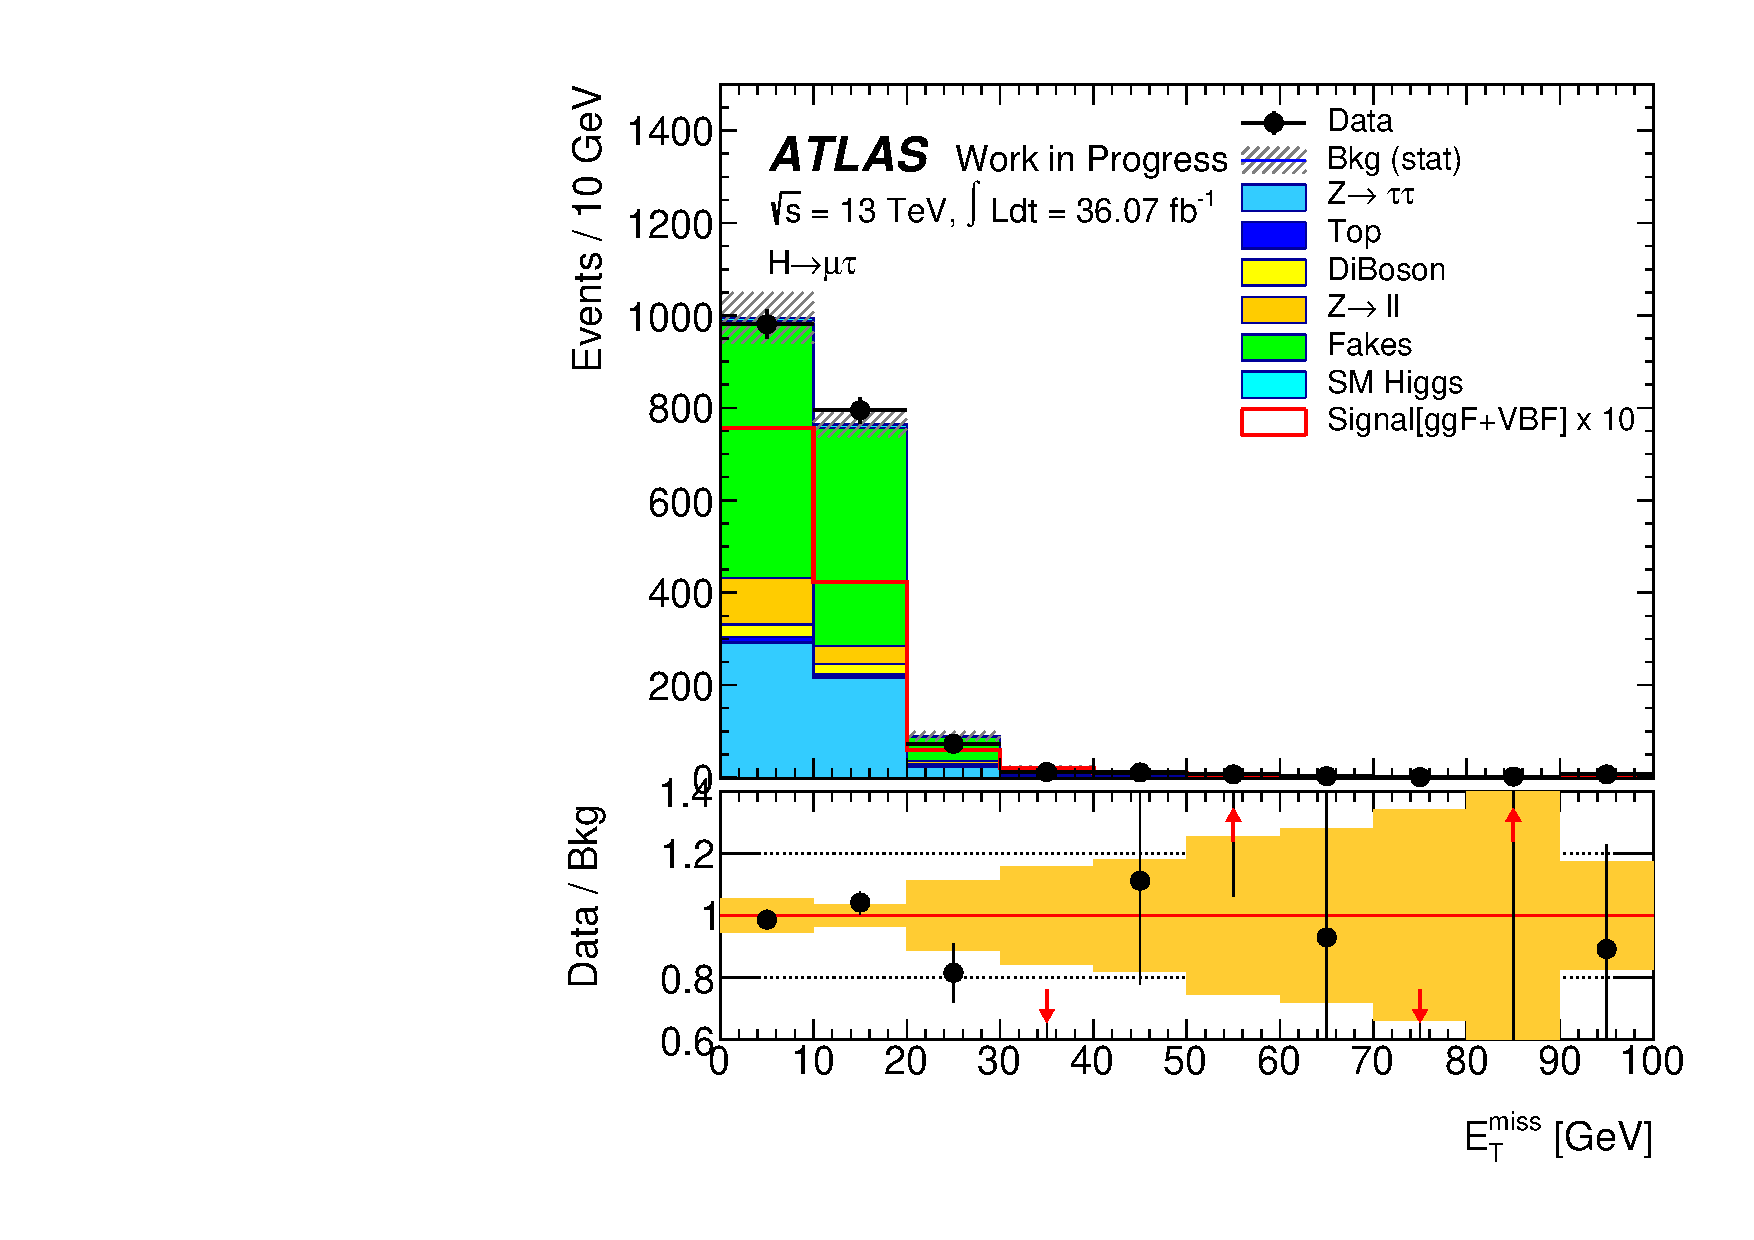
\includegraphics[width=.30\textwidth,height=.30\textheight,type=pdf,ext=.pdf,read=.pdf]{/afs/cern.ch/user/a/atpathak/afswork/public/Pixel/LFV_Plots/Plots_Qframework_25Apr2018_Final_note/plots_mcZll/mtau-CutTauMTSR2_VBF-met-lin}\\
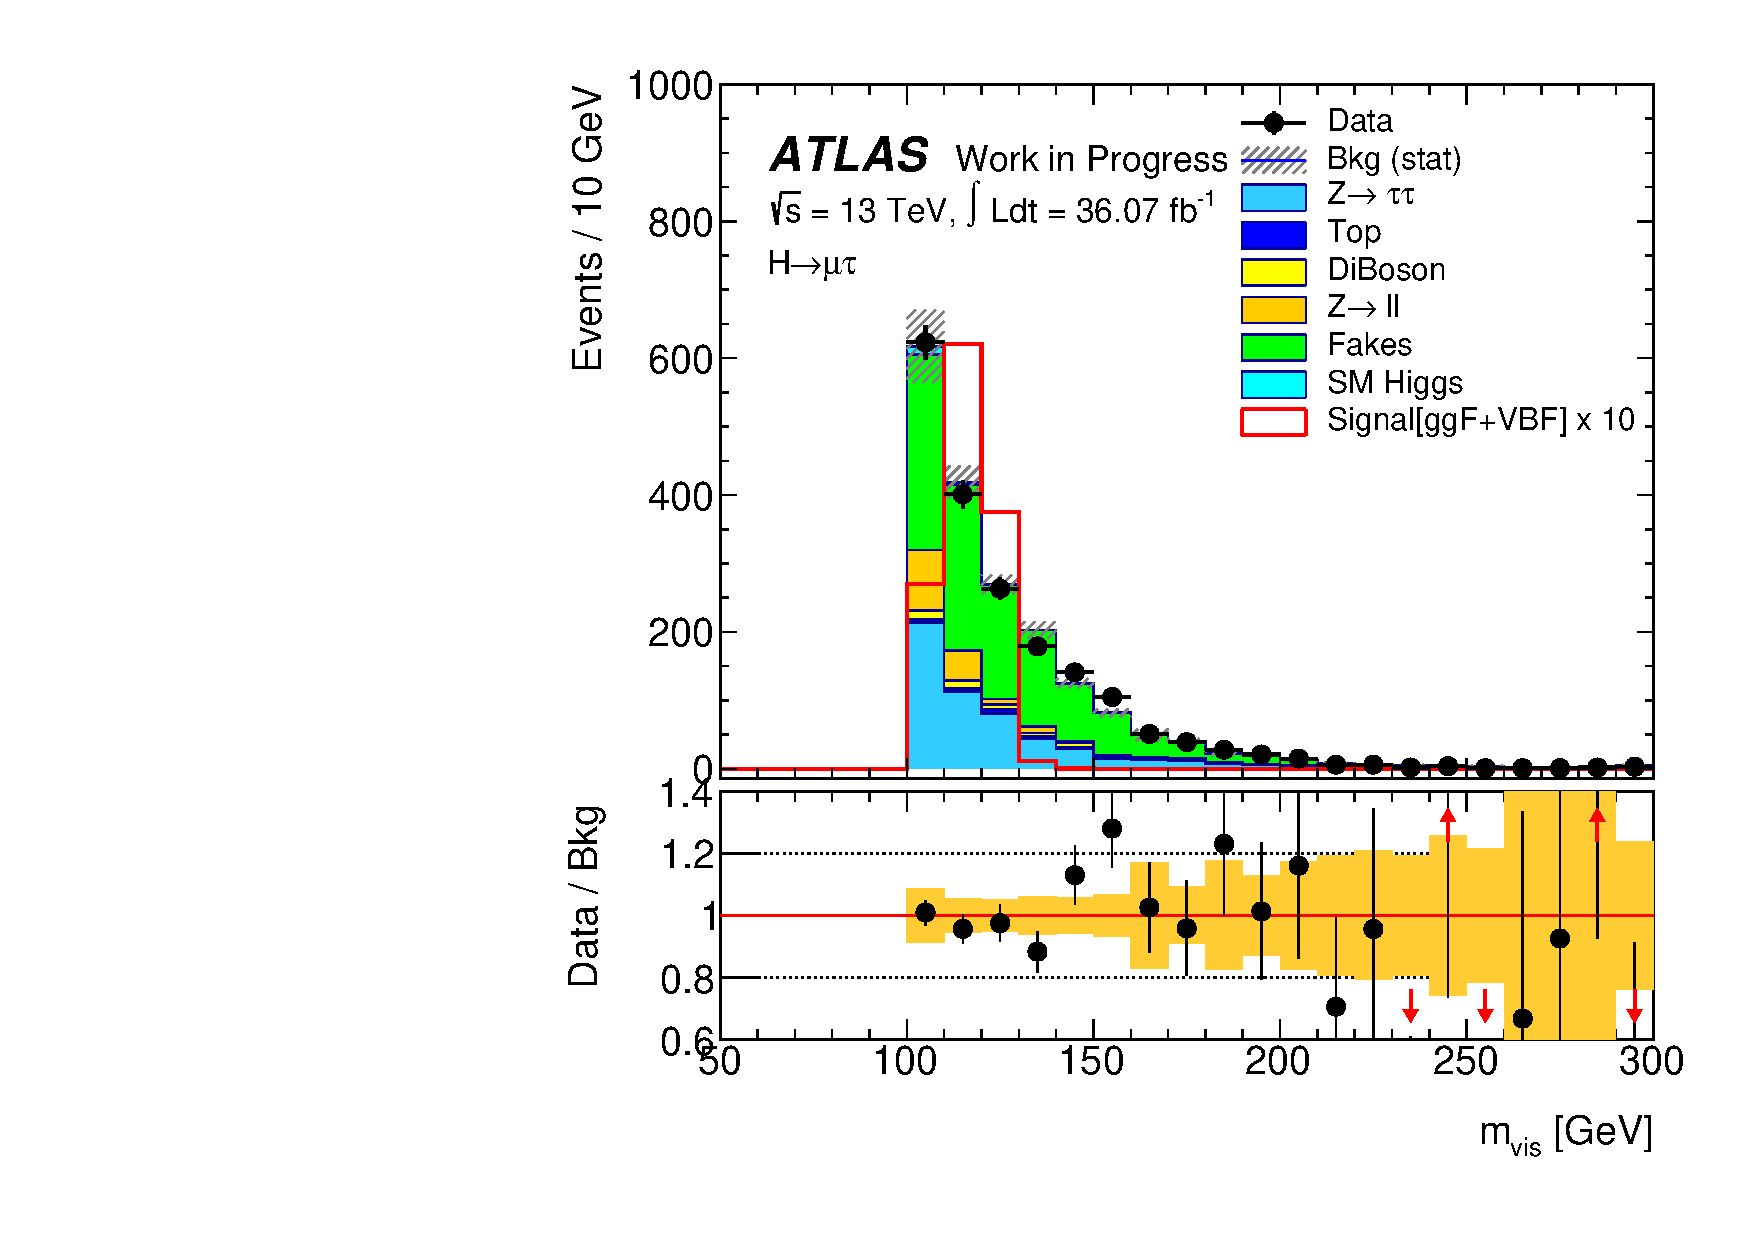
\includegraphics[width=.30\textwidth,height=.30\textheight,type=pdf,ext=.pdf,read=.pdf]{/afs/cern.ch/user/a/atpathak/afswork/public/Pixel/LFV_Plots/Plots_Qframework_25Apr2018_Final_note/plots_mcZll/mtau-CutTauMTSR2_VBF-visibleMass-lin}
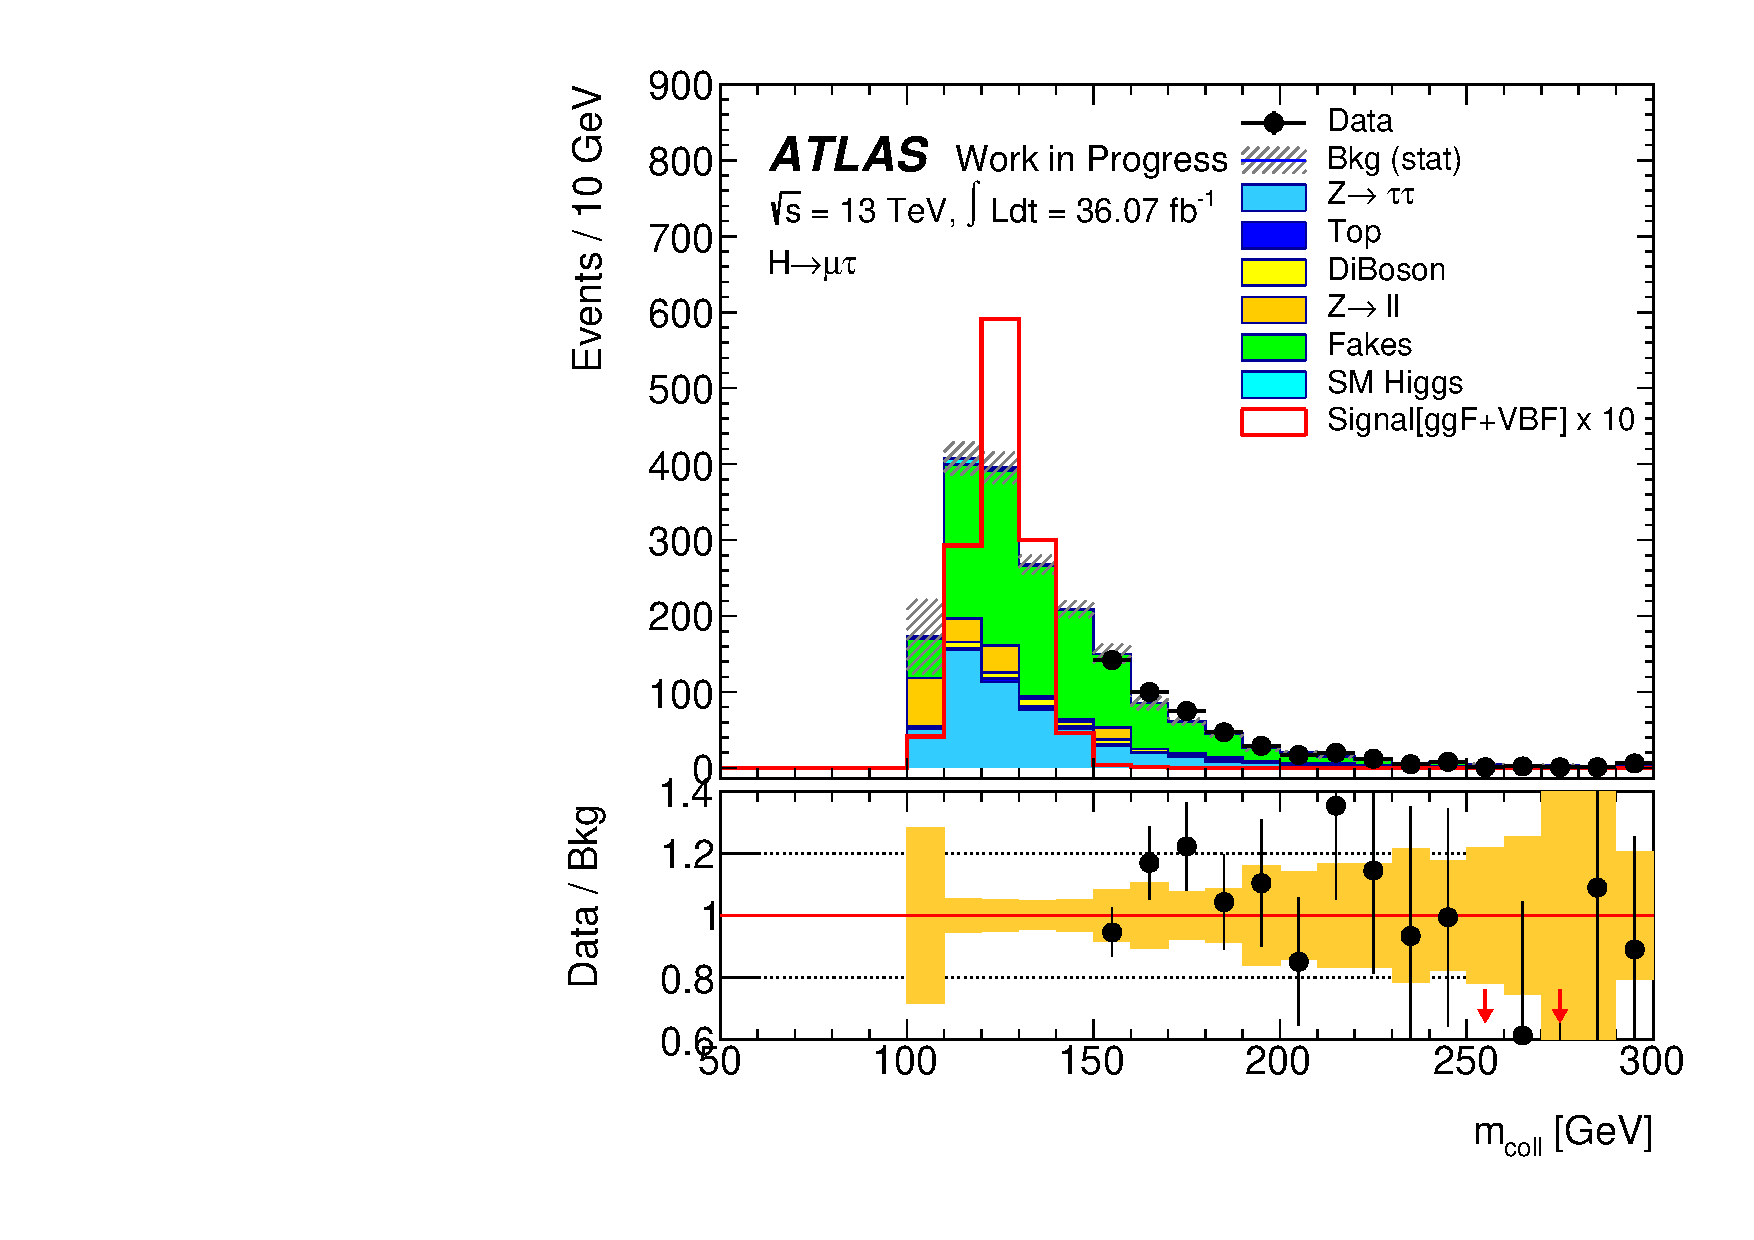
\includegraphics[width=.30\textwidth,height=.30\textheight,type=pdf,ext=.pdf,read=.pdf]{/afs/cern.ch/user/a/atpathak/afswork/public/Pixel/LFV_Plots/Plots_Qframework_25Apr2018_Final_note/plots_mcZll/mtau-CutTauMTSR2_VBF-collMassBL-lin}
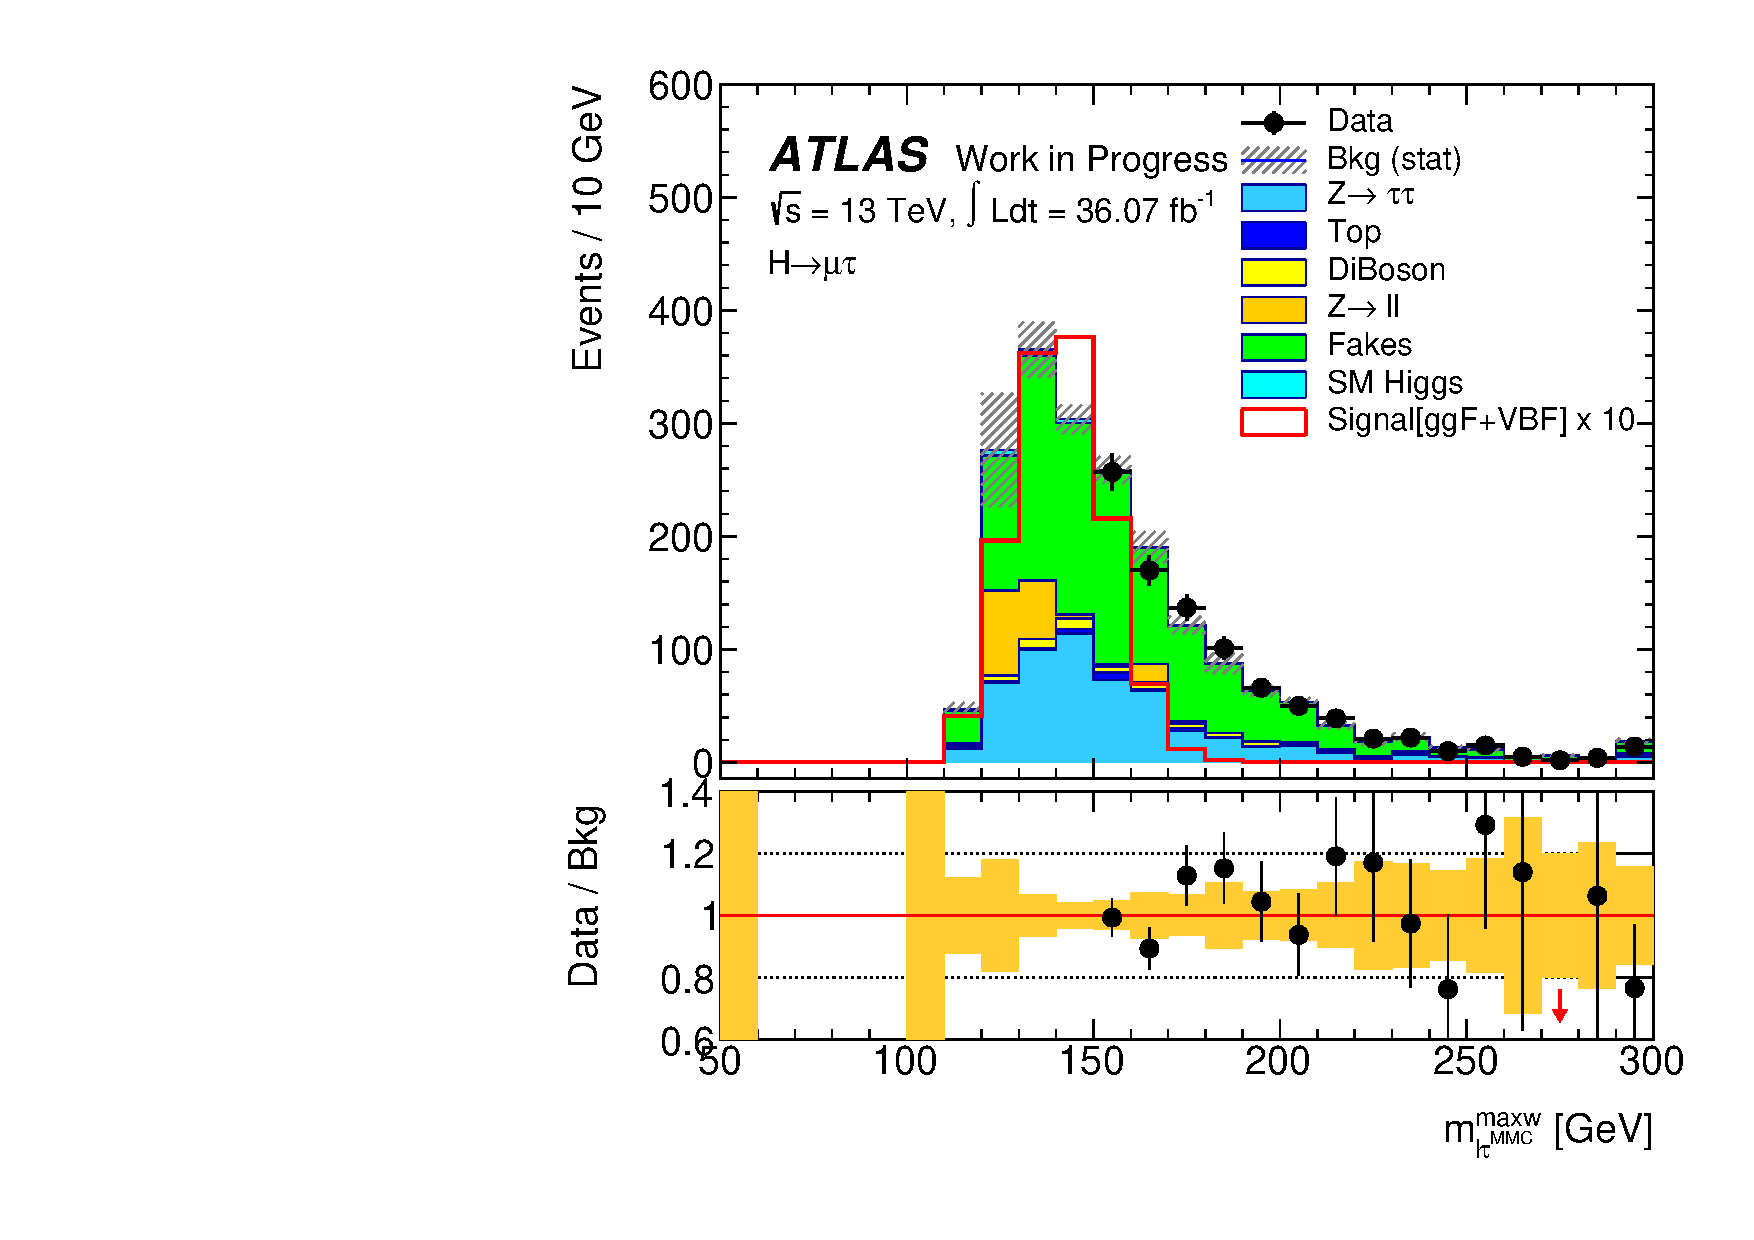
\includegraphics[width=.30\textwidth,height=.30\textheight,type=pdf,ext=.pdf,read=.pdf]{/afs/cern.ch/user/a/atpathak/afswork/public/Pixel/LFV_Plots/Plots_Qframework_25Apr2018_Final_note/plots_mcZll/mtau-CutTauMTSR2_VBF-MMCBL-lin}
\end{normalsize}
\end{frame}
%-----------------------------------------------
\begin{frame}
\frametitle{Distributions of $\mu\tau_{had}$ events in the SR3' region.}
\begin{normalsize}
\vspace*{0.2cm}
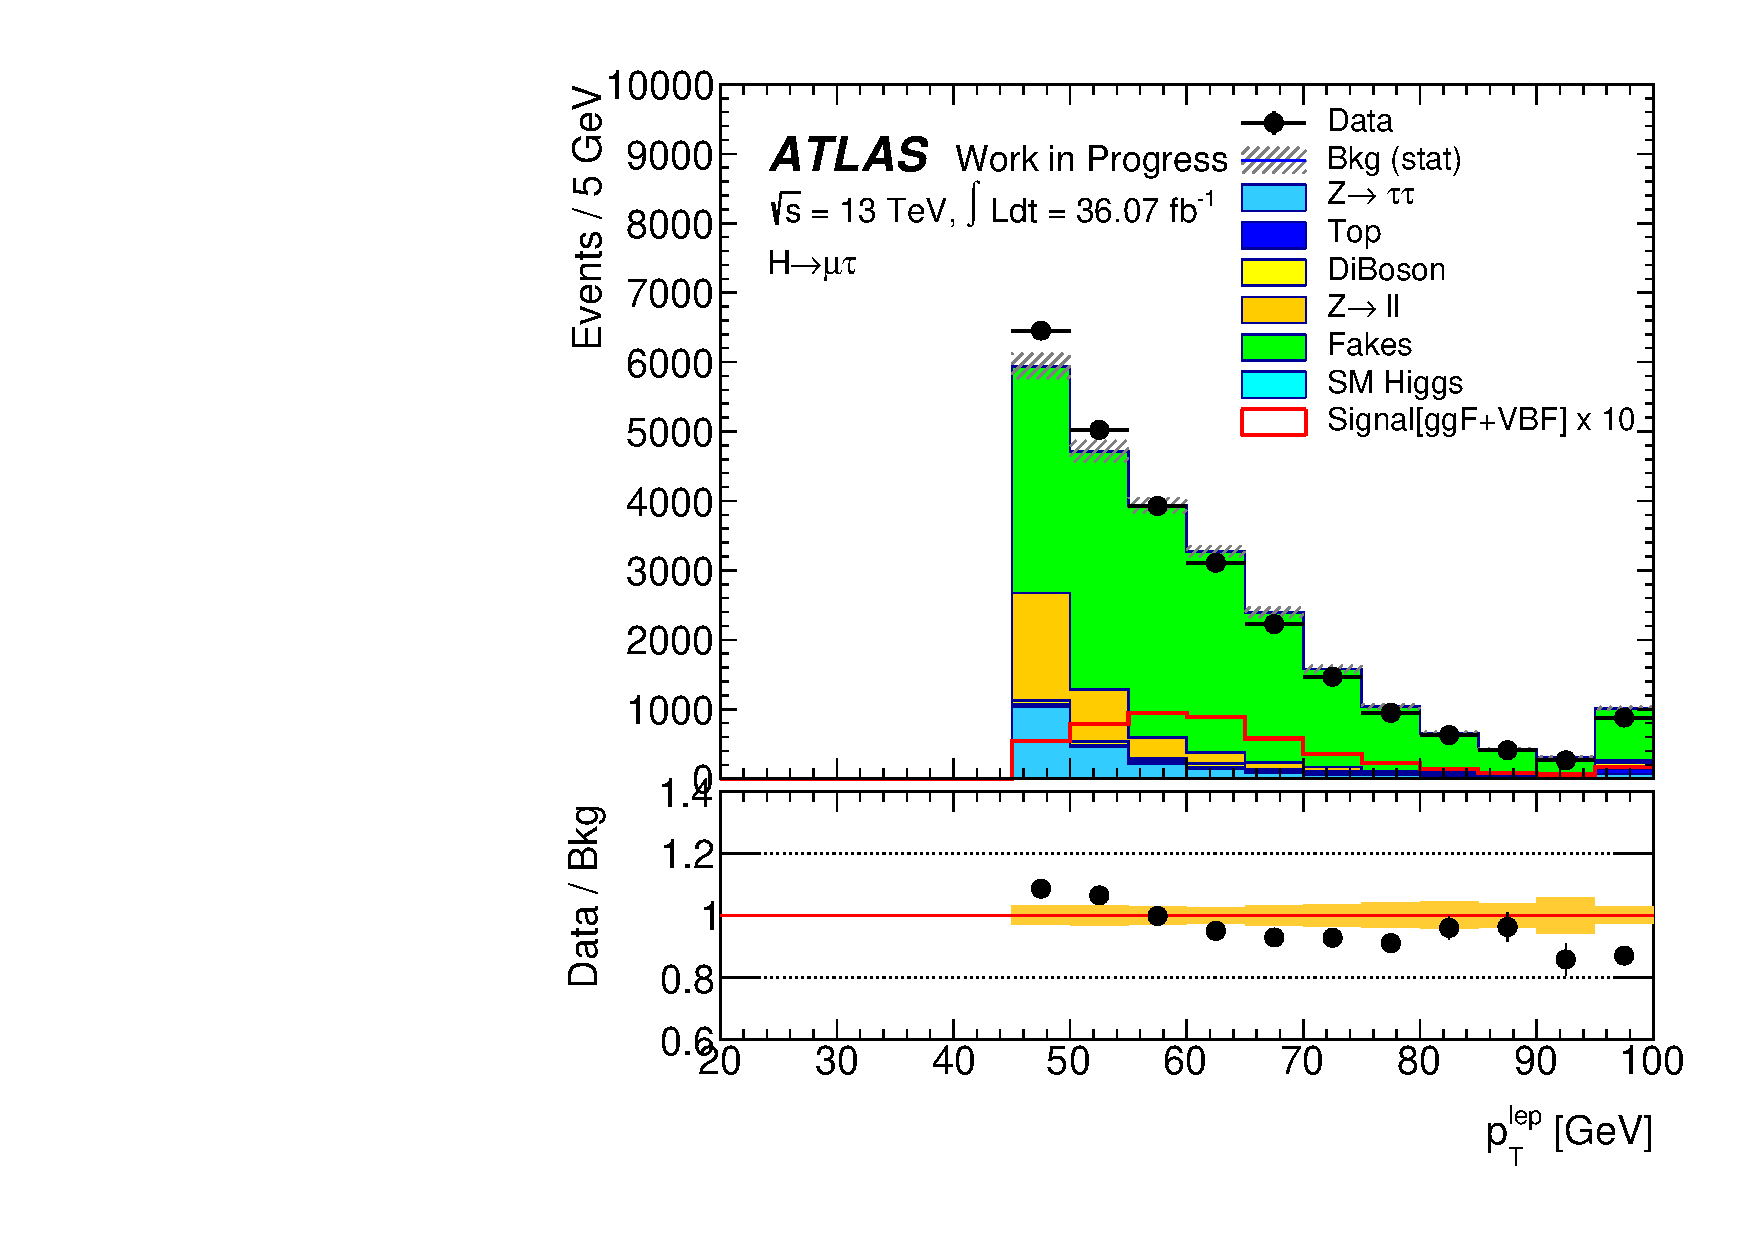
\includegraphics[width=.30\textwidth,height=.30\textheight,type=pdf,ext=.pdf,read=.pdf]{/afs/cern.ch/user/a/atpathak/afswork/public/Pixel/LFV_Plots/Plots_Qframework_25Apr2018_Final_note/plots_mcZll/mtau-CutTauPtSR3_VBF-leptonPt-lin}
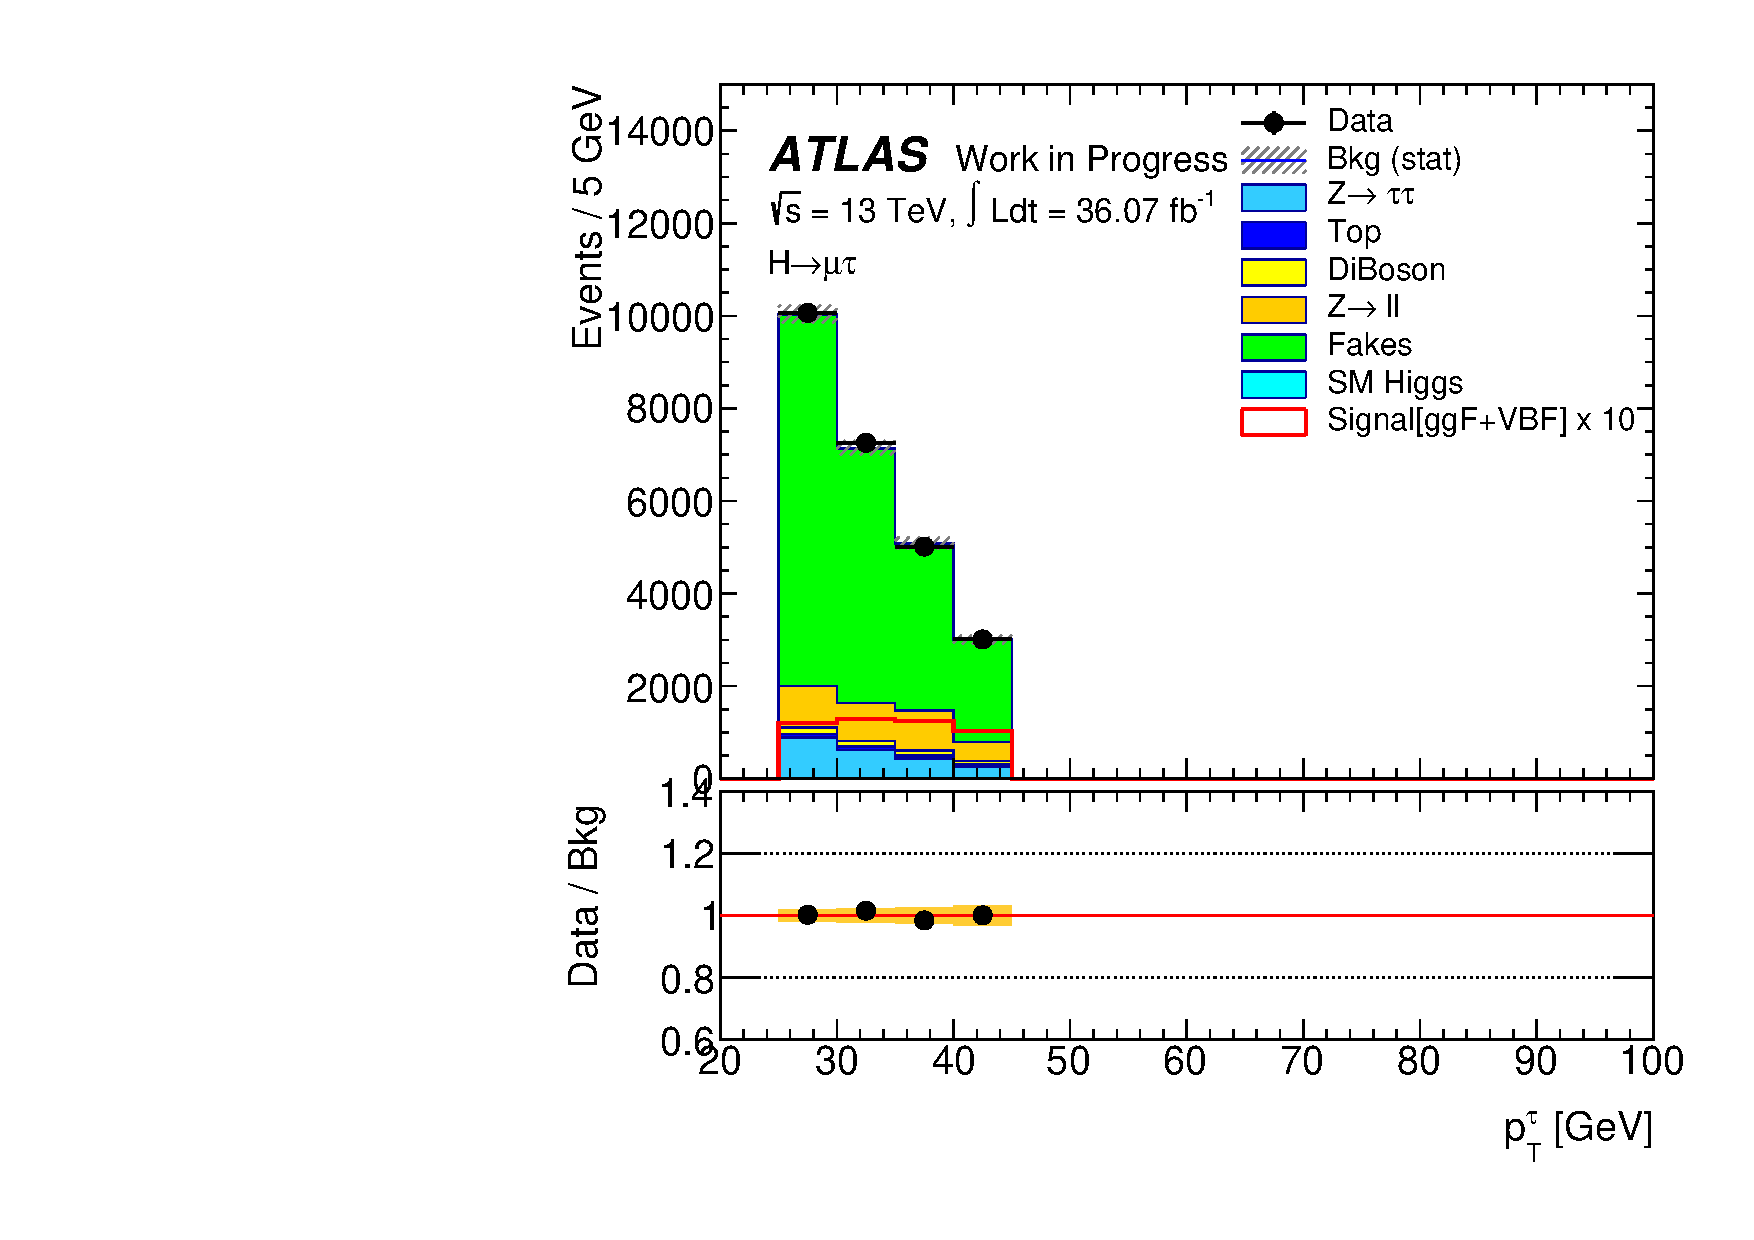
\includegraphics[width=.30\textwidth,height=.30\textheight,type=pdf,ext=.pdf,read=.pdf]{/afs/cern.ch/user/a/atpathak/afswork/public/Pixel/LFV_Plots/Plots_Qframework_25Apr2018_Final_note/plots_mcZll/mtau-CutTauPtSR3_VBF-tauPt-lin}
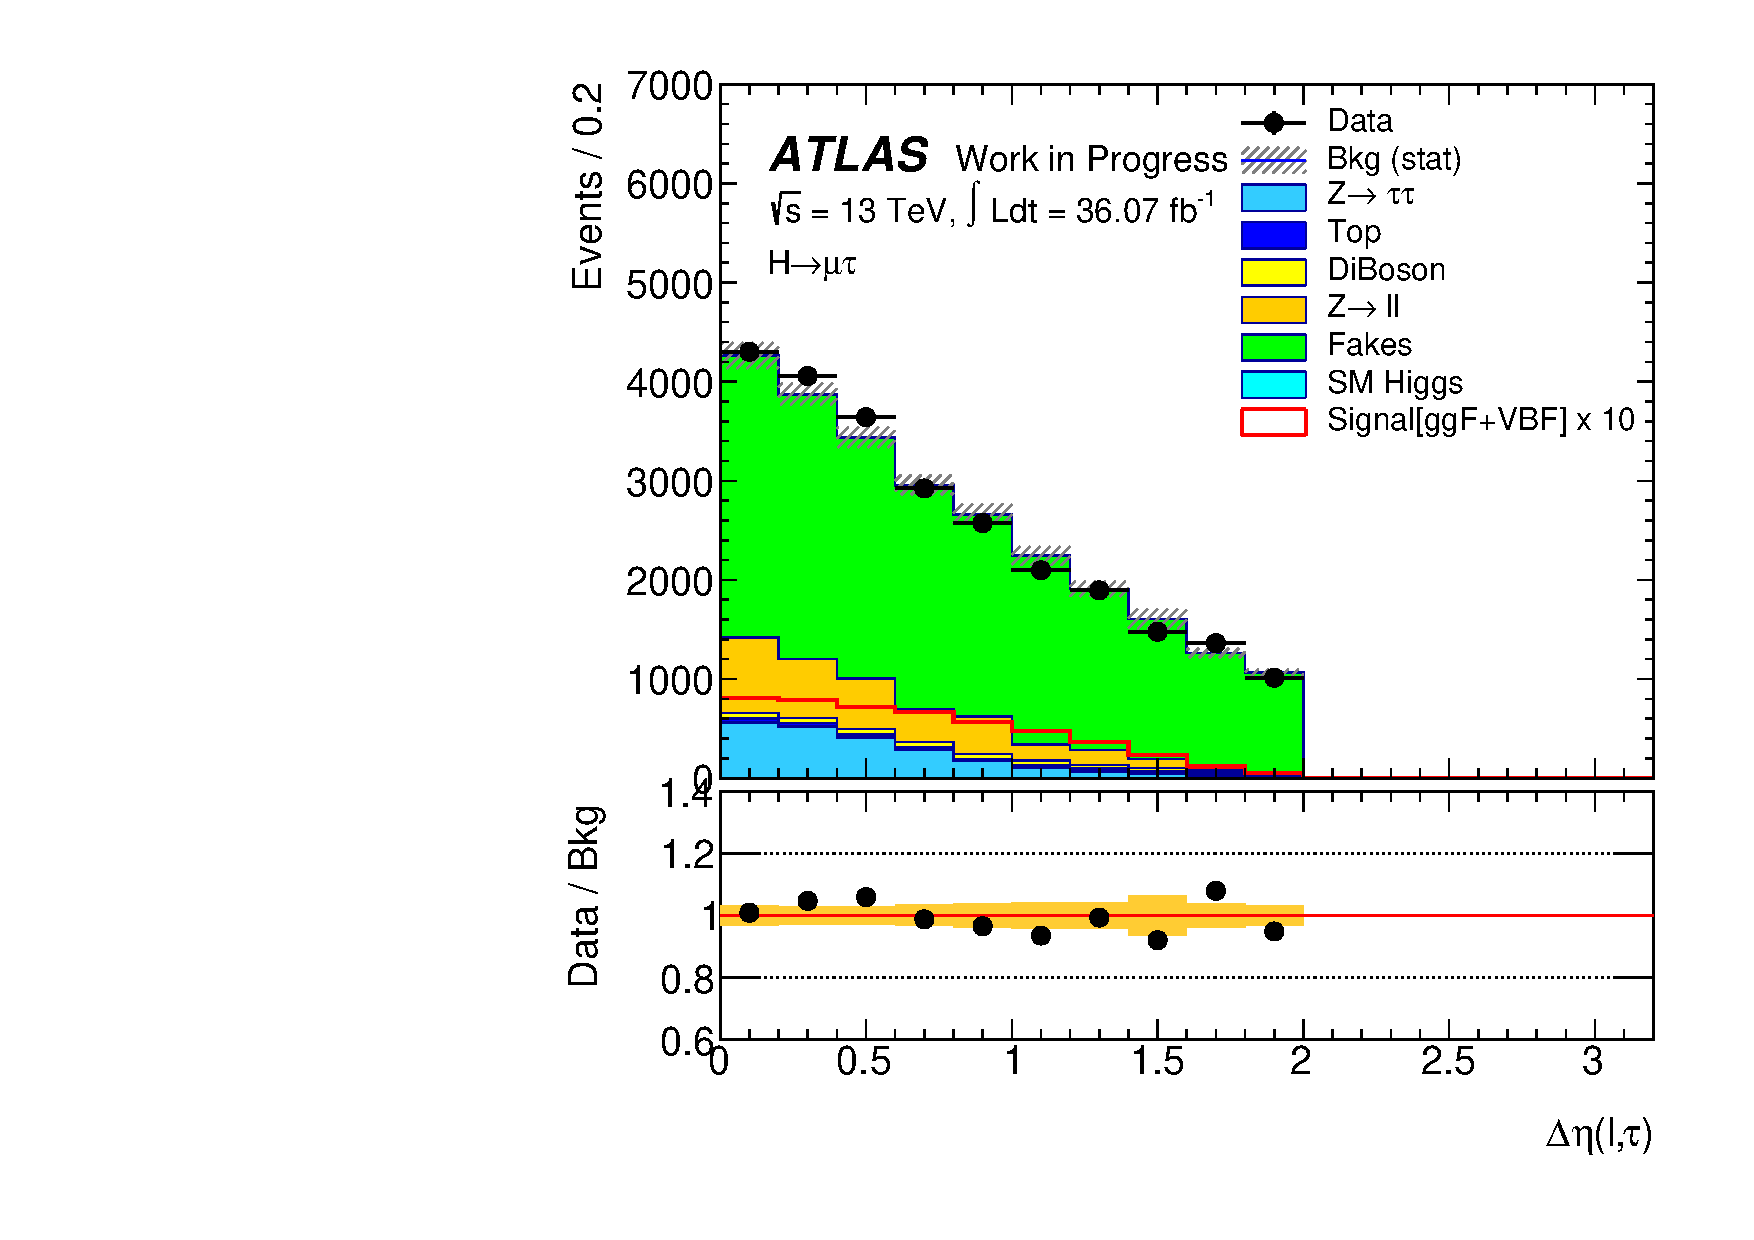
\includegraphics[width=.30\textwidth,height=.30\textheight,type=pdf,ext=.pdf,read=.pdf]{/afs/cern.ch/user/a/atpathak/afswork/public/Pixel/LFV_Plots/Plots_Qframework_25Apr2018_Final_note/plots_mcZll/mtau-CutTauPtSR3_VBF-dEtaTauLep-lin}\\
\includegraphics[width=.30\textwidth,height=.30\textheight,type=pdf,ext=.pdf,read=.pdf]{/afs/cern.ch/user/a/atpathak/afswork/public/Pixel/LFV_Plots/Plots_Qframework_25Apr2018_Final_note/plots_mcZll/mtau-CutTauPtSR3_VBF-transverseMassLepMET-lin}
\includegraphics[width=.30\textwidth,height=.30\textheight,type=pdf,ext=.pdf,read=.pdf]{/afs/cern.ch/user/a/atpathak/afswork/public/Pixel/LFV_Plots/Plots_Qframework_25Apr2018_Final_note/plots_mcZll/mtau-CutTauPtSR3_VBF-transverseMassTauMET-lin}
\includegraphics[width=.30\textwidth,height=.30\textheight,type=pdf,ext=.pdf,read=.pdf]{/afs/cern.ch/user/a/atpathak/afswork/public/Pixel/LFV_Plots/Plots_Qframework_25Apr2018_Final_note/plots_mcZll/mtau-CutTauPtSR3_VBF-met-lin}\\
\includegraphics[width=.30\textwidth,height=.30\textheight,type=pdf,ext=.pdf,read=.pdf]{/afs/cern.ch/user/a/atpathak/afswork/public/Pixel/LFV_Plots/Plots_Qframework_25Apr2018_Final_note/plots_mcZll/mtau-CutTauPtSR3_VBF-visibleMass-lin}
\includegraphics[width=.30\textwidth,height=.30\textheight,type=pdf,ext=.pdf,read=.pdf]{/afs/cern.ch/user/a/atpathak/afswork/public/Pixel/LFV_Plots/Plots_Qframework_25Apr2018_Final_note/plots_mcZll/mtau-CutTauPtSR3_VBF-collMassBL-lin}
\includegraphics[width=.30\textwidth,height=.30\textheight,type=pdf,ext=.pdf,read=.pdf]{/afs/cern.ch/user/a/atpathak/afswork/public/Pixel/LFV_Plots/Plots_Qframework_25Apr2018_Final_note/plots_mcZll/mtau-CutTauPtSR3_VBF-MMCBL-lin}
\end{normalsize}
\end{frame}
%-----------------------------------------------
\begin{frame}
\frametitle{Distributions of $\mu\tau_{had}$ events in the VBF region.}
\begin{normalsize}
\vspace*{0.2cm}
\includegraphics[width=.30\textwidth,height=.30\textheight,type=pdf,ext=.pdf,read=.pdf]{/afs/cern.ch/user/a/atpathak/afswork/public/Pixel/LFV_Plots/Plots_Qframework_25Apr2018_Final_note/plots_mcZll/mtau-CutVBF-leptonPt-lin}
\includegraphics[width=.30\textwidth,height=.30\textheight,type=pdf,ext=.pdf,read=.pdf]{/afs/cern.ch/user/a/atpathak/afswork/public/Pixel/LFV_Plots/Plots_Qframework_25Apr2018_Final_note/plots_mcZll/mtau-CutVBF-tauPt-lin}
\includegraphics[width=.30\textwidth,height=.30\textheight,type=pdf,ext=.pdf,read=.pdf]{/afs/cern.ch/user/a/atpathak/afswork/public/Pixel/LFV_Plots/Plots_Qframework_25Apr2018_Final_note/plots_mcZll/mtau-CutVBF-dEtaTauLep-lin}\\
\includegraphics[width=.30\textwidth,height=.30\textheight,type=pdf,ext=.pdf,read=.pdf]{/afs/cern.ch/user/a/atpathak/afswork/public/Pixel/LFV_Plots/Plots_Qframework_25Apr2018_Final_note/plots_mcZll/mtau-CutVBF-transverseMassLepMET-lin}
\includegraphics[width=.30\textwidth,height=.30\textheight,type=pdf,ext=.pdf,read=.pdf]{/afs/cern.ch/user/a/atpathak/afswork/public/Pixel/LFV_Plots/Plots_Qframework_25Apr2018_Final_note/plots_mcZll/mtau-CutVBF-transverseMassTauMET-lin}
\includegraphics[width=.30\textwidth,height=.30\textheight,type=pdf,ext=.pdf,read=.pdf]{/afs/cern.ch/user/a/atpathak/afswork/public/Pixel/LFV_Plots/Plots_Qframework_25Apr2018_Final_note/plots_mcZll/mtau-CutVBF-met-lin}\\
\includegraphics[width=.30\textwidth,height=.30\textheight,type=pdf,ext=.pdf,read=.pdf]{/afs/cern.ch/user/a/atpathak/afswork/public/Pixel/LFV_Plots/Plots_Qframework_25Apr2018_Final_note/plots_mcZll/mtau-CutVBF-visibleMass-lin}
\includegraphics[width=.30\textwidth,height=.30\textheight,type=pdf,ext=.pdf,read=.pdf]{/afs/cern.ch/user/a/atpathak/afswork/public/Pixel/LFV_Plots/Plots_Qframework_25Apr2018_Final_note/plots_mcZll/mtau-CutVBF-collMassBL-lin}
\includegraphics[width=.30\textwidth,height=.30\textheight,type=pdf,ext=.pdf,read=.pdf]{/afs/cern.ch/user/a/atpathak/afswork/public/Pixel/LFV_Plots/Plots_Qframework_25Apr2018_Final_note/plots_mcZll/mtau-CutVBF-MMCBL-lin}
\end{normalsize}
\end{frame}
%-----------------------------------------------
\begin{frame}
\frametitle{Distributions of $\mu\tau_{had}$ events in the WCR region.}
\begin{normalsize}
\vspace*{0.2cm}
\includegraphics[width=.30\textwidth,height=.30\textheight,type=pdf,ext=.pdf,read=.pdf]{/afs/cern.ch/user/a/atpathak/afswork/public/Pixel/LFV_Plots/Plots_Qframework_25Apr2018_Final_note/plots_mcZll/mtau-CutWCR-leptonPt-lin}
\includegraphics[width=.30\textwidth,height=.30\textheight,type=pdf,ext=.pdf,read=.pdf]{/afs/cern.ch/user/a/atpathak/afswork/public/Pixel/LFV_Plots/Plots_Qframework_25Apr2018_Final_note/plots_mcZll/mtau-CutWCR-tauPt-lin}
\includegraphics[width=.30\textwidth,height=.30\textheight,type=pdf,ext=.pdf,read=.pdf]{/afs/cern.ch/user/a/atpathak/afswork/public/Pixel/LFV_Plots/Plots_Qframework_25Apr2018_Final_note/plots_mcZll/mtau-CutWCR-dEtaTauLep-lin}\\
\includegraphics[width=.30\textwidth,height=.30\textheight,type=pdf,ext=.pdf,read=.pdf]{/afs/cern.ch/user/a/atpathak/afswork/public/Pixel/LFV_Plots/Plots_Qframework_25Apr2018_Final_note/plots_mcZll/mtau-CutWCR-transverseMassLepMET-lin}
\includegraphics[width=.30\textwidth,height=.30\textheight,type=pdf,ext=.pdf,read=.pdf]{/afs/cern.ch/user/a/atpathak/afswork/public/Pixel/LFV_Plots/Plots_Qframework_25Apr2018_Final_note/plots_mcZll/mtau-CutWCR-transverseMassTauMET-lin}
\includegraphics[width=.30\textwidth,height=.30\textheight,type=pdf,ext=.pdf,read=.pdf]{/afs/cern.ch/user/a/atpathak/afswork/public/Pixel/LFV_Plots/Plots_Qframework_25Apr2018_Final_note/plots_mcZll/mtau-CutWCR-met-lin}\\
\includegraphics[width=.30\textwidth,height=.30\textheight,type=pdf,ext=.pdf,read=.pdf]{/afs/cern.ch/user/a/atpathak/afswork/public/Pixel/LFV_Plots/Plots_Qframework_25Apr2018_Final_note/plots_mcZll/mtau-CutWCR-visibleMass-lin}
\includegraphics[width=.30\textwidth,height=.30\textheight,type=pdf,ext=.pdf,read=.pdf]{/afs/cern.ch/user/a/atpathak/afswork/public/Pixel/LFV_Plots/Plots_Qframework_25Apr2018_Final_note/plots_mcZll/mtau-CutWCR-collMassBL-lin}
\includegraphics[width=.30\textwidth,height=.30\textheight,type=pdf,ext=.pdf,read=.pdf]{/afs/cern.ch/user/a/atpathak/afswork/public/Pixel/LFV_Plots/Plots_Qframework_25Apr2018_Final_note/plots_mcZll/mtau-CutWCR-MMCBL-lin}
\end{normalsize}
\end{frame}
%-----------------------------------------------
\begin{frame}
\frametitle{Distributions of $\mu\tau_{had}$ events in the Top validation region.}
\begin{normalsize}
\vspace*{0.2cm}
\includegraphics[width=.30\textwidth,height=.30\textheight,type=pdf,ext=.pdf,read=.pdf]{/afs/cern.ch/user/a/atpathak/afswork/public/Pixel/LFV_Plots/Plots_Qframework_25Apr2018_Final_note/plots_mcZll/mtau-CutTopCR-leptonPt-lin}
\includegraphics[width=.30\textwidth,height=.30\textheight,type=pdf,ext=.pdf,read=.pdf]{/afs/cern.ch/user/a/atpathak/afswork/public/Pixel/LFV_Plots/Plots_Qframework_25Apr2018_Final_note/plots_mcZll/mtau-CutTopCR-tauPt-lin}
\includegraphics[width=.30\textwidth,height=.30\textheight,type=pdf,ext=.pdf,read=.pdf]{/afs/cern.ch/user/a/atpathak/afswork/public/Pixel/LFV_Plots/Plots_Qframework_25Apr2018_Final_note/plots_mcZll/mtau-CutTopCR-dEtaTauLep-lin}\\
\includegraphics[width=.30\textwidth,height=.30\textheight,type=pdf,ext=.pdf,read=.pdf]{/afs/cern.ch/user/a/atpathak/afswork/public/Pixel/LFV_Plots/Plots_Qframework_25Apr2018_Final_note/plots_mcZll/mtau-CutTopCR-transverseMassLepMET-lin}
\includegraphics[width=.30\textwidth,height=.30\textheight,type=pdf,ext=.pdf,read=.pdf]{/afs/cern.ch/user/a/atpathak/afswork/public/Pixel/LFV_Plots/Plots_Qframework_25Apr2018_Final_note/plots_mcZll/mtau-CutTopCR-transverseMassTauMET-lin}
\includegraphics[width=.30\textwidth,height=.30\textheight,type=pdf,ext=.pdf,read=.pdf]{/afs/cern.ch/user/a/atpathak/afswork/public/Pixel/LFV_Plots/Plots_Qframework_25Apr2018_Final_note/plots_mcZll/mtau-CutTopCR-met-lin}\\
\includegraphics[width=.30\textwidth,height=.30\textheight,type=pdf,ext=.pdf,read=.pdf]{/afs/cern.ch/user/a/atpathak/afswork/public/Pixel/LFV_Plots/Plots_Qframework_25Apr2018_Final_note/plots_mcZll/mtau-CutTopCR-visibleMass-lin}
\includegraphics[width=.30\textwidth,height=.30\textheight,type=pdf,ext=.pdf,read=.pdf]{/afs/cern.ch/user/a/atpathak/afswork/public/Pixel/LFV_Plots/Plots_Qframework_25Apr2018_Final_note/plots_mcZll/mtau-CutTopCR-collMassBL-lin}
\includegraphics[width=.30\textwidth,height=.30\textheight,type=pdf,ext=.pdf,read=.pdf]{/afs/cern.ch/user/a/atpathak/afswork/public/Pixel/LFV_Plots/Plots_Qframework_25Apr2018_Final_note/plots_mcZll/mtau-CutTopCR-MMCBL-lin}
\end{normalsize}
\end{frame}
%-----------------------------------------------
\begin{frame}
\frametitle{Distributions of $\mu\tau_{had}$ events in the QCDCR region.}
\begin{normalsize}
\vspace*{0.2cm}
\includegraphics[width=.30\textwidth,height=.30\textheight,type=pdf,ext=.pdf,read=.pdf]{/afs/cern.ch/user/a/atpathak/afswork/public/Pixel/LFV_Plots/Plots_Qframework_25Apr2018_Final_note/plots_mcZll/mtau-CutQCDCR-leptonPt-lin}
\includegraphics[width=.30\textwidth,height=.30\textheight,type=pdf,ext=.pdf,read=.pdf]{/afs/cern.ch/user/a/atpathak/afswork/public/Pixel/LFV_Plots/Plots_Qframework_25Apr2018_Final_note/plots_mcZll/mtau-CutQCDCR-tauPt-lin}
\includegraphics[width=.30\textwidth,height=.30\textheight,type=pdf,ext=.pdf,read=.pdf]{/afs/cern.ch/user/a/atpathak/afswork/public/Pixel/LFV_Plots/Plots_Qframework_25Apr2018_Final_note/plots_mcZll/mtau-CutQCDCR-dEtaTauLep-lin}\\
\includegraphics[width=.30\textwidth,height=.30\textheight,type=pdf,ext=.pdf,read=.pdf]{/afs/cern.ch/user/a/atpathak/afswork/public/Pixel/LFV_Plots/Plots_Qframework_25Apr2018_Final_note/plots_mcZll/mtau-CutQCDCR-transverseMassLepMET-lin}
\includegraphics[width=.30\textwidth,height=.30\textheight,type=pdf,ext=.pdf,read=.pdf]{/afs/cern.ch/user/a/atpathak/afswork/public/Pixel/LFV_Plots/Plots_Qframework_25Apr2018_Final_note/plots_mcZll/mtau-CutQCDCR-transverseMassTauMET-lin}
\includegraphics[width=.30\textwidth,height=.30\textheight,type=pdf,ext=.pdf,read=.pdf]{/afs/cern.ch/user/a/atpathak/afswork/public/Pixel/LFV_Plots/Plots_Qframework_25Apr2018_Final_note/plots_mcZll/mtau-CutQCDCR-met-lin}\\
\includegraphics[width=.30\textwidth,height=.30\textheight,type=pdf,ext=.pdf,read=.pdf]{/afs/cern.ch/user/a/atpathak/afswork/public/Pixel/LFV_Plots/Plots_Qframework_25Apr2018_Final_note/plots_mcZll/mtau-CutQCDCR-visibleMass-lin}
\includegraphics[width=.30\textwidth,height=.30\textheight,type=pdf,ext=.pdf,read=.pdf]{/afs/cern.ch/user/a/atpathak/afswork/public/Pixel/LFV_Plots/Plots_Qframework_25Apr2018_Final_note/plots_mcZll/mtau-CutQCDCR-collMassBL-lin}
\includegraphics[width=.30\textwidth,height=.30\textheight,type=pdf,ext=.pdf,read=.pdf]{/afs/cern.ch/user/a/atpathak/afswork/public/Pixel/LFV_Plots/Plots_Qframework_25Apr2018_Final_note/plots_mcZll/mtau-CutQCDCR-MMCBL-lin}
\end{normalsize}
\end{frame}
%-----------------------------------------------
\begin{frame}
\frametitle{Distributions of $\mu\tau_{had}$ events in the QCDCR2 region.}
\begin{normalsize}
\vspace*{0.2cm}
\includegraphics[width=.30\textwidth,height=.30\textheight,type=pdf,ext=.pdf,read=.pdf]{/afs/cern.ch/user/a/atpathak/afswork/public/Pixel/LFV_Plots/Plots_Qframework_25Apr2018_Final_note/plots_mcZll/mtau-CutQCDCR2-leptonPt-lin}
\includegraphics[width=.30\textwidth,height=.30\textheight,type=pdf,ext=.pdf,read=.pdf]{/afs/cern.ch/user/a/atpathak/afswork/public/Pixel/LFV_Plots/Plots_Qframework_25Apr2018_Final_note/plots_mcZll/mtau-CutQCDCR2-tauPt-lin}
\includegraphics[width=.30\textwidth,height=.30\textheight,type=pdf,ext=.pdf,read=.pdf]{/afs/cern.ch/user/a/atpathak/afswork/public/Pixel/LFV_Plots/Plots_Qframework_25Apr2018_Final_note/plots_mcZll/mtau-CutQCDCR2-dEtaTauLep-lin}\\
\includegraphics[width=.30\textwidth,height=.30\textheight,type=pdf,ext=.pdf,read=.pdf]{/afs/cern.ch/user/a/atpathak/afswork/public/Pixel/LFV_Plots/Plots_Qframework_25Apr2018_Final_note/plots_mcZll/mtau-CutQCDCR2-transverseMassLepMET-lin}
\includegraphics[width=.30\textwidth,height=.30\textheight,type=pdf,ext=.pdf,read=.pdf]{/afs/cern.ch/user/a/atpathak/afswork/public/Pixel/LFV_Plots/Plots_Qframework_25Apr2018_Final_note/plots_mcZll/mtau-CutQCDCR2-transverseMassTauMET-lin}
\includegraphics[width=.30\textwidth,height=.30\textheight,type=pdf,ext=.pdf,read=.pdf]{/afs/cern.ch/user/a/atpathak/afswork/public/Pixel/LFV_Plots/Plots_Qframework_25Apr2018_Final_note/plots_mcZll/mtau-CutQCDCR2-met-lin}\\
\includegraphics[width=.30\textwidth,height=.30\textheight,type=pdf,ext=.pdf,read=.pdf]{/afs/cern.ch/user/a/atpathak/afswork/public/Pixel/LFV_Plots/Plots_Qframework_25Apr2018_Final_note/plots_mcZll/mtau-CutQCDCR2-visibleMass-lin}
\includegraphics[width=.30\textwidth,height=.30\textheight,type=pdf,ext=.pdf,read=.pdf]{/afs/cern.ch/user/a/atpathak/afswork/public/Pixel/LFV_Plots/Plots_Qframework_25Apr2018_Final_note/plots_mcZll/mtau-CutQCDCR2-collMassBL-lin}
\includegraphics[width=.30\textwidth,height=.30\textheight,type=pdf,ext=.pdf,read=.pdf]{/afs/cern.ch/user/a/atpathak/afswork/public/Pixel/LFV_Plots/Plots_Qframework_25Apr2018_Final_note/plots_mcZll/mtau-CutQCDCR2-MMCBL-lin}
\end{normalsize}
\end{frame}
%-----------------------------------------------
\begin{frame}
\frametitle{Distributions of $\mu\tau_{had}$ events in the Z$\tau^{+}\tau^{-}$   region.}
\begin{normalsize}
\vspace*{0.2cm}
\includegraphics[width=.30\textwidth,height=.30\textheight,type=pdf,ext=.pdf,read=.pdf]{/afs/cern.ch/user/a/atpathak/afswork/public/Pixel/LFV_Plots/Plots_Qframework_25Apr2018_Final_note/plots_mcZll/mtau-CutZttCR-leptonPt-lin}
\includegraphics[width=.30\textwidth,height=.30\textheight,type=pdf,ext=.pdf,read=.pdf]{/afs/cern.ch/user/a/atpathak/afswork/public/Pixel/LFV_Plots/Plots_Qframework_25Apr2018_Final_note/plots_mcZll/mtau-CutZttCR-tauPt-lin}
\includegraphics[width=.30\textwidth,height=.30\textheight,type=pdf,ext=.pdf,read=.pdf]{/afs/cern.ch/user/a/atpathak/afswork/public/Pixel/LFV_Plots/Plots_Qframework_25Apr2018_Final_note/plots_mcZll/mtau-CutZttCR-dEtaTauLep-lin}\\
\includegraphics[width=.30\textwidth,height=.30\textheight,type=pdf,ext=.pdf,read=.pdf]{/afs/cern.ch/user/a/atpathak/afswork/public/Pixel/LFV_Plots/Plots_Qframework_25Apr2018_Final_note/plots_mcZll/mtau-CutZttCR-transverseMassLepMET-lin}
\includegraphics[width=.30\textwidth,height=.30\textheight,type=pdf,ext=.pdf,read=.pdf]{/afs/cern.ch/user/a/atpathak/afswork/public/Pixel/LFV_Plots/Plots_Qframework_25Apr2018_Final_note/plots_mcZll/mtau-CutZttCR-transverseMassTauMET-lin}
\includegraphics[width=.30\textwidth,height=.30\textheight,type=pdf,ext=.pdf,read=.pdf]{/afs/cern.ch/user/a/atpathak/afswork/public/Pixel/LFV_Plots/Plots_Qframework_25Apr2018_Final_note/plots_mcZll/mtau-CutZttCR-met-lin}\\
\includegraphics[width=.30\textwidth,height=.30\textheight,type=pdf,ext=.pdf,read=.pdf]{/afs/cern.ch/user/a/atpathak/afswork/public/Pixel/LFV_Plots/Plots_Qframework_25Apr2018_Final_note/plots_mcZll/mtau-CutZttCR-visibleMass-lin}
\includegraphics[width=.30\textwidth,height=.30\textheight,type=pdf,ext=.pdf,read=.pdf]{/afs/cern.ch/user/a/atpathak/afswork/public/Pixel/LFV_Plots/Plots_Qframework_25Apr2018_Final_note/plots_mcZll/mtau-CutZttCR-collMassBL-lin}
\includegraphics[width=.30\textwidth,height=.30\textheight,type=pdf,ext=.pdf,read=.pdf]{/afs/cern.ch/user/a/atpathak/afswork/public/Pixel/LFV_Plots/Plots_Qframework_25Apr2018_Final_note/plots_mcZll/mtau-CutZttCR-MMCBL-lin}
\end{normalsize}
\end{frame}
%-----------------------------------------------
\begin{frame}
\frametitle{Distributions of $e\tau_{had}$ events in the SR1 region.}
\begin{normalsize}
\vspace*{0.2cm}
\includegraphics[width=.30\textwidth,height=.30\textheight,type=pdf,ext=.pdf,read=.pdf]{/afs/cern.ch/user/a/atpathak/afswork/public/Pixel/LFV_Plots/Plots_Qframework_25Apr2018_Final_note/plots_mcZll/etau-CutTauMTSR1-leptonPt-lin}
\includegraphics[width=.30\textwidth,height=.30\textheight,type=pdf,ext=.pdf,read=.pdf]{/afs/cern.ch/user/a/atpathak/afswork/public/Pixel/LFV_Plots/Plots_Qframework_25Apr2018_Final_note/plots_mcZll/etau-CutTauMTSR1-tauPt-lin}
\includegraphics[width=.30\textwidth,height=.30\textheight,type=pdf,ext=.pdf,read=.pdf]{/afs/cern.ch/user/a/atpathak/afswork/public/Pixel/LFV_Plots/Plots_Qframework_25Apr2018_Final_note/plots_mcZll/etau-CutTauMTSR1-dEtaTauLep-lin}\\
\includegraphics[width=.30\textwidth,height=.30\textheight,type=pdf,ext=.pdf,read=.pdf]{/afs/cern.ch/user/a/atpathak/afswork/public/Pixel/LFV_Plots/Plots_Qframework_25Apr2018_Final_note/plots_mcZll/etau-CutTauMTSR1-transverseMassLepMET-lin}
\includegraphics[width=.30\textwidth,height=.30\textheight,type=pdf,ext=.pdf,read=.pdf]{/afs/cern.ch/user/a/atpathak/afswork/public/Pixel/LFV_Plots/Plots_Qframework_25Apr2018_Final_note/plots_mcZll/etau-CutTauMTSR1-transverseMassTauMET-lin}
\includegraphics[width=.30\textwidth,height=.30\textheight,type=pdf,ext=.pdf,read=.pdf]{/afs/cern.ch/user/a/atpathak/afswork/public/Pixel/LFV_Plots/Plots_Qframework_25Apr2018_Final_note/plots_mcZll/etau-CutTauMTSR1-met-lin}\\
\includegraphics[width=.30\textwidth,height=.30\textheight,type=pdf,ext=.pdf,read=.pdf]{/afs/cern.ch/user/a/atpathak/afswork/public/Pixel/LFV_Plots/Plots_Qframework_25Apr2018_Final_note/plots_mcZll/etau-CutTauMTSR1-visibleMass-lin}
\includegraphics[width=.30\textwidth,height=.30\textheight,type=pdf,ext=.pdf,read=.pdf]{/afs/cern.ch/user/a/atpathak/afswork/public/Pixel/LFV_Plots/Plots_Qframework_25Apr2018_Final_note/plots_mcZll/etau-CutTauMTSR1-collMassBL-lin}
\includegraphics[width=.30\textwidth,height=.30\textheight,type=pdf,ext=.pdf,read=.pdf]{/afs/cern.ch/user/a/atpathak/afswork/public/Pixel/LFV_Plots/Plots_Qframework_25Apr2018_Final_note/plots_mcZll/etau-CutTauMTSR1-MMCBL-lin}
\end{normalsize}
\end{frame}
%-----------------------------------------------
\begin{frame}
\frametitle{Distributions of $e\tau_{had}$ events in the SR2 region(mvis cut).}
\begin{normalsize}
\vspace*{0.2cm}
\includegraphics[width=.30\textwidth,height=.30\textheight,type=pdf,ext=.pdf,read=.pdf]{/afs/cern.ch/user/a/atpathak/afswork/public/Pixel/LFV_Plots/Plots_Qframework_25Apr2018_Final_note/plots_mcZll/etau-CutTauMTSR2_Mvis-leptonPt-lin}
\includegraphics[width=.30\textwidth,height=.30\textheight,type=pdf,ext=.pdf,read=.pdf]{/afs/cern.ch/user/a/atpathak/afswork/public/Pixel/LFV_Plots/Plots_Qframework_25Apr2018_Final_note/plots_mcZll/etau-CutTauMTSR2_Mvis-tauPt-lin}
\includegraphics[width=.30\textwidth,height=.30\textheight,type=pdf,ext=.pdf,read=.pdf]{/afs/cern.ch/user/a/atpathak/afswork/public/Pixel/LFV_Plots/Plots_Qframework_25Apr2018_Final_note/plots_mcZll/etau-CutTauMTSR2_Mvis-dEtaTauLep-lin}\\
\includegraphics[width=.30\textwidth,height=.30\textheight,type=pdf,ext=.pdf,read=.pdf]{/afs/cern.ch/user/a/atpathak/afswork/public/Pixel/LFV_Plots/Plots_Qframework_25Apr2018_Final_note/plots_mcZll/etau-CutTauMTSR2_Mvis-transverseMassLepMET-lin}
\includegraphics[width=.30\textwidth,height=.30\textheight,type=pdf,ext=.pdf,read=.pdf]{/afs/cern.ch/user/a/atpathak/afswork/public/Pixel/LFV_Plots/Plots_Qframework_25Apr2018_Final_note/plots_mcZll/etau-CutTauMTSR2_Mvis-transverseMassTauMET-lin}
\includegraphics[width=.30\textwidth,height=.30\textheight,type=pdf,ext=.pdf,read=.pdf]{/afs/cern.ch/user/a/atpathak/afswork/public/Pixel/LFV_Plots/Plots_Qframework_25Apr2018_Final_note/plots_mcZll/etau-CutTauMTSR2_Mvis-met-lin}\\
\includegraphics[width=.30\textwidth,height=.30\textheight,type=pdf,ext=.pdf,read=.pdf]{/afs/cern.ch/user/a/atpathak/afswork/public/Pixel/LFV_Plots/Plots_Qframework_25Apr2018_Final_note/plots_mcZll/etau-CutTauMTSR2_Mvis-visibleMass-lin}
\includegraphics[width=.30\textwidth,height=.30\textheight,type=pdf,ext=.pdf,read=.pdf]{/afs/cern.ch/user/a/atpathak/afswork/public/Pixel/LFV_Plots/Plots_Qframework_25Apr2018_Final_note/plots_mcZll/etau-CutTauMTSR2_Mvis-collMassBL-lin}
\includegraphics[width=.30\textwidth,height=.30\textheight,type=pdf,ext=.pdf,read=.pdf]{/afs/cern.ch/user/a/atpathak/afswork/public/Pixel/LFV_Plots/Plots_Qframework_25Apr2018_Final_note/plots_mcZll/etau-CutTauMTSR2_Mvis-MMCBL-lin}
\end{normalsize}
\end{frame}
%-----------------------------------------------
\begin{frame}
\frametitle{Distributions of $e\tau_{had}$ events in the SR3 region.}
\begin{normalsize}
\vspace*{0.2cm}
\includegraphics[width=.30\textwidth,height=.30\textheight,type=pdf,ext=.pdf,read=.pdf]{/afs/cern.ch/user/a/atpathak/afswork/public/Pixel/LFV_Plots/Plots_Qframework_25Apr2018_Final_note/plots_mcZll/etau-CutTauPtSR3-leptonPt-lin}
\includegraphics[width=.30\textwidth,height=.30\textheight,type=pdf,ext=.pdf,read=.pdf]{/afs/cern.ch/user/a/atpathak/afswork/public/Pixel/LFV_Plots/Plots_Qframework_25Apr2018_Final_note/plots_mcZll/etau-CutTauPtSR3-tauPt-lin}
\includegraphics[width=.30\textwidth,height=.30\textheight,type=pdf,ext=.pdf,read=.pdf]{/afs/cern.ch/user/a/atpathak/afswork/public/Pixel/LFV_Plots/Plots_Qframework_25Apr2018_Final_note/plots_mcZll/etau-CutTauPtSR3-dEtaTauLep-lin}\\
\includegraphics[width=.30\textwidth,height=.30\textheight,type=pdf,ext=.pdf,read=.pdf]{/afs/cern.ch/user/a/atpathak/afswork/public/Pixel/LFV_Plots/Plots_Qframework_25Apr2018_Final_note/plots_mcZll/etau-CutTauPtSR3-transverseMassLepMET-lin}
\includegraphics[width=.30\textwidth,height=.30\textheight,type=pdf,ext=.pdf,read=.pdf]{/afs/cern.ch/user/a/atpathak/afswork/public/Pixel/LFV_Plots/Plots_Qframework_25Apr2018_Final_note/plots_mcZll/etau-CutTauPtSR3-transverseMassTauMET-lin}
\includegraphics[width=.30\textwidth,height=.30\textheight,type=pdf,ext=.pdf,read=.pdf]{/afs/cern.ch/user/a/atpathak/afswork/public/Pixel/LFV_Plots/Plots_Qframework_25Apr2018_Final_note/plots_mcZll/etau-CutTauPtSR3-met-lin}\\
\includegraphics[width=.30\textwidth,height=.30\textheight,type=pdf,ext=.pdf,read=.pdf]{/afs/cern.ch/user/a/atpathak/afswork/public/Pixel/LFV_Plots/Plots_Qframework_25Apr2018_Final_note/plots_mcZll/etau-CutTauPtSR3-visibleMass-lin}
\includegraphics[width=.30\textwidth,height=.30\textheight,type=pdf,ext=.pdf,read=.pdf]{/afs/cern.ch/user/a/atpathak/afswork/public/Pixel/LFV_Plots/Plots_Qframework_25Apr2018_Final_note/plots_mcZll/etau-CutTauPtSR3-collMassBL-lin}
\includegraphics[width=.30\textwidth,height=.30\textheight,type=pdf,ext=.pdf,read=.pdf]{/afs/cern.ch/user/a/atpathak/afswork/public/Pixel/LFV_Plots/Plots_Qframework_25Apr2018_Final_note/plots_mcZll/etau-CutTauPtSR3-MMCBL-lin}
\end{normalsize}
\end{frame}
%-----------------------------------------------
\begin{frame}
\frametitle{Distributions of $e\tau_{had}$ events in the SR1' region.}
\begin{normalsize}
\vspace*{0.2cm}
\includegraphics[width=.30\textwidth,height=.30\textheight,type=pdf,ext=.pdf,read=.pdf]{/afs/cern.ch/user/a/atpathak/afswork/public/Pixel/LFV_Plots/Plots_Qframework_25Apr2018_Final_note/plots_mcZll/etau-CutTauMTSR1_VBF-leptonPt-lin}
\includegraphics[width=.30\textwidth,height=.30\textheight,type=pdf,ext=.pdf,read=.pdf]{/afs/cern.ch/user/a/atpathak/afswork/public/Pixel/LFV_Plots/Plots_Qframework_25Apr2018_Final_note/plots_mcZll/etau-CutTauMTSR1_VBF-tauPt-lin}
\includegraphics[width=.30\textwidth,height=.30\textheight,type=pdf,ext=.pdf,read=.pdf]{/afs/cern.ch/user/a/atpathak/afswork/public/Pixel/LFV_Plots/Plots_Qframework_25Apr2018_Final_note/plots_mcZll/etau-CutTauMTSR1_VBF-dEtaTauLep-lin}\\
\includegraphics[width=.30\textwidth,height=.30\textheight,type=pdf,ext=.pdf,read=.pdf]{/afs/cern.ch/user/a/atpathak/afswork/public/Pixel/LFV_Plots/Plots_Qframework_25Apr2018_Final_note/plots_mcZll/etau-CutTauMTSR1_VBF-transverseMassLepMET-lin}
\includegraphics[width=.30\textwidth,height=.30\textheight,type=pdf,ext=.pdf,read=.pdf]{/afs/cern.ch/user/a/atpathak/afswork/public/Pixel/LFV_Plots/Plots_Qframework_25Apr2018_Final_note/plots_mcZll/etau-CutTauMTSR1_VBF-transverseMassTauMET-lin}
\includegraphics[width=.30\textwidth,height=.30\textheight,type=pdf,ext=.pdf,read=.pdf]{/afs/cern.ch/user/a/atpathak/afswork/public/Pixel/LFV_Plots/Plots_Qframework_25Apr2018_Final_note/plots_mcZll/etau-CutTauMTSR1_VBF-met-lin}\\
\includegraphics[width=.30\textwidth,height=.30\textheight,type=pdf,ext=.pdf,read=.pdf]{/afs/cern.ch/user/a/atpathak/afswork/public/Pixel/LFV_Plots/Plots_Qframework_25Apr2018_Final_note/plots_mcZll/etau-CutTauMTSR1_VBF-visibleMass-lin}
\includegraphics[width=.30\textwidth,height=.30\textheight,type=pdf,ext=.pdf,read=.pdf]{/afs/cern.ch/user/a/atpathak/afswork/public/Pixel/LFV_Plots/Plots_Qframework_25Apr2018_Final_note/plots_mcZll/etau-CutTauMTSR1_VBF-collMassBL-lin}
\includegraphics[width=.30\textwidth,height=.30\textheight,type=pdf,ext=.pdf,read=.pdf]{/afs/cern.ch/user/a/atpathak/afswork/public/Pixel/LFV_Plots/Plots_Qframework_25Apr2018_Final_note/plots_mcZll/etau-CutTauMTSR1_VBF-MMCBL-lin}
\end{normalsize}
\end{frame}
%-----------------------------------------------
\begin{frame}
\frametitle{Distributions of $e\tau_{had}$ events in the SR2' region.}
\begin{normalsize}
\vspace*{0.2cm}
\includegraphics[width=.30\textwidth,height=.30\textheight,type=pdf,ext=.pdf,read=.pdf]{/afs/cern.ch/user/a/atpathak/afswork/public/Pixel/LFV_Plots/Plots_Qframework_25Apr2018_Final_note/plots_mcZll/etau-CutTauMTSR2_VBF-leptonPt-lin}
\includegraphics[width=.30\textwidth,height=.30\textheight,type=pdf,ext=.pdf,read=.pdf]{/afs/cern.ch/user/a/atpathak/afswork/public/Pixel/LFV_Plots/Plots_Qframework_25Apr2018_Final_note/plots_mcZll/etau-CutTauMTSR2_VBF-tauPt-lin}
\includegraphics[width=.30\textwidth,height=.30\textheight,type=pdf,ext=.pdf,read=.pdf]{/afs/cern.ch/user/a/atpathak/afswork/public/Pixel/LFV_Plots/Plots_Qframework_25Apr2018_Final_note/plots_mcZll/etau-CutTauMTSR2_VBF-dEtaTauLep-lin}\\
\includegraphics[width=.30\textwidth,height=.30\textheight,type=pdf,ext=.pdf,read=.pdf]{/afs/cern.ch/user/a/atpathak/afswork/public/Pixel/LFV_Plots/Plots_Qframework_25Apr2018_Final_note/plots_mcZll/etau-CutTauMTSR2_VBF-transverseMassLepMET-lin}
\includegraphics[width=.30\textwidth,height=.30\textheight,type=pdf,ext=.pdf,read=.pdf]{/afs/cern.ch/user/a/atpathak/afswork/public/Pixel/LFV_Plots/Plots_Qframework_25Apr2018_Final_note/plots_mcZll/etau-CutTauMTSR2_VBF-transverseMassTauMET-lin}
\includegraphics[width=.30\textwidth,height=.30\textheight,type=pdf,ext=.pdf,read=.pdf]{/afs/cern.ch/user/a/atpathak/afswork/public/Pixel/LFV_Plots/Plots_Qframework_25Apr2018_Final_note/plots_mcZll/etau-CutTauMTSR2_VBF-met-lin}\\
\includegraphics[width=.30\textwidth,height=.30\textheight,type=pdf,ext=.pdf,read=.pdf]{/afs/cern.ch/user/a/atpathak/afswork/public/Pixel/LFV_Plots/Plots_Qframework_25Apr2018_Final_note/plots_mcZll/etau-CutTauMTSR2_VBF-visibleMass-lin}
\includegraphics[width=.30\textwidth,height=.30\textheight,type=pdf,ext=.pdf,read=.pdf]{/afs/cern.ch/user/a/atpathak/afswork/public/Pixel/LFV_Plots/Plots_Qframework_25Apr2018_Final_note/plots_mcZll/etau-CutTauMTSR2_VBF-collMassBL-lin}
\includegraphics[width=.30\textwidth,height=.30\textheight,type=pdf,ext=.pdf,read=.pdf]{/afs/cern.ch/user/a/atpathak/afswork/public/Pixel/LFV_Plots/Plots_Qframework_25Apr2018_Final_note/plots_mcZll/etau-CutTauMTSR2_VBF-MMCBL-lin}
\end{normalsize}
\end{frame}
%-----------------------------------------------
\begin{frame}
\frametitle{Distributions of $e\tau_{had}$ events in the SR3' region.}
\begin{normalsize}
\vspace*{0.2cm}
\includegraphics[width=.30\textwidth,height=.30\textheight,type=pdf,ext=.pdf,read=.pdf]{/afs/cern.ch/user/a/atpathak/afswork/public/Pixel/LFV_Plots/Plots_Qframework_25Apr2018_Final_note/plots_mcZll/etau-CutTauPtSR3_VBF-leptonPt-lin}
\includegraphics[width=.30\textwidth,height=.30\textheight,type=pdf,ext=.pdf,read=.pdf]{/afs/cern.ch/user/a/atpathak/afswork/public/Pixel/LFV_Plots/Plots_Qframework_25Apr2018_Final_note/plots_mcZll/etau-CutTauPtSR3_VBF-tauPt-lin}
\includegraphics[width=.30\textwidth,height=.30\textheight,type=pdf,ext=.pdf,read=.pdf]{/afs/cern.ch/user/a/atpathak/afswork/public/Pixel/LFV_Plots/Plots_Qframework_25Apr2018_Final_note/plots_mcZll/etau-CutTauPtSR3_VBF-dEtaTauLep-lin}\\
\includegraphics[width=.30\textwidth,height=.30\textheight,type=pdf,ext=.pdf,read=.pdf]{/afs/cern.ch/user/a/atpathak/afswork/public/Pixel/LFV_Plots/Plots_Qframework_25Apr2018_Final_note/plots_mcZll/etau-CutTauPtSR3_VBF-transverseMassLepMET-lin}
\includegraphics[width=.30\textwidth,height=.30\textheight,type=pdf,ext=.pdf,read=.pdf]{/afs/cern.ch/user/a/atpathak/afswork/public/Pixel/LFV_Plots/Plots_Qframework_25Apr2018_Final_note/plots_mcZll/etau-CutTauPtSR3_VBF-transverseMassTauMET-lin}
\includegraphics[width=.30\textwidth,height=.30\textheight,type=pdf,ext=.pdf,read=.pdf]{/afs/cern.ch/user/a/atpathak/afswork/public/Pixel/LFV_Plots/Plots_Qframework_25Apr2018_Final_note/plots_mcZll/etau-CutTauPtSR3_VBF-met-lin}\\
\includegraphics[width=.30\textwidth,height=.30\textheight,type=pdf,ext=.pdf,read=.pdf]{/afs/cern.ch/user/a/atpathak/afswork/public/Pixel/LFV_Plots/Plots_Qframework_25Apr2018_Final_note/plots_mcZll/etau-CutTauPtSR3_VBF-visibleMass-lin}
\includegraphics[width=.30\textwidth,height=.30\textheight,type=pdf,ext=.pdf,read=.pdf]{/afs/cern.ch/user/a/atpathak/afswork/public/Pixel/LFV_Plots/Plots_Qframework_25Apr2018_Final_note/plots_mcZll/etau-CutTauPtSR3_VBF-collMassBL-lin}
\includegraphics[width=.30\textwidth,height=.30\textheight,type=pdf,ext=.pdf,read=.pdf]{/afs/cern.ch/user/a/atpathak/afswork/public/Pixel/LFV_Plots/Plots_Qframework_25Apr2018_Final_note/plots_mcZll/etau-CutTauPtSR3_VBF-MMCBL-lin}
\end{normalsize}
\end{frame}
%-----------------------------------------------
\begin{frame}
\frametitle{Distributions of $e\tau_{had}$ events in the VBF region.}
\begin{normalsize}
\vspace*{0.2cm}
\includegraphics[width=.30\textwidth,height=.30\textheight,type=pdf,ext=.pdf,read=.pdf]{/afs/cern.ch/user/a/atpathak/afswork/public/Pixel/LFV_Plots/Plots_Qframework_25Apr2018_Final_note/plots_mcZll/etau-CutVBF-leptonPt-lin}
\includegraphics[width=.30\textwidth,height=.30\textheight,type=pdf,ext=.pdf,read=.pdf]{/afs/cern.ch/user/a/atpathak/afswork/public/Pixel/LFV_Plots/Plots_Qframework_25Apr2018_Final_note/plots_mcZll/etau-CutVBF-tauPt-lin}
\includegraphics[width=.30\textwidth,height=.30\textheight,type=pdf,ext=.pdf,read=.pdf]{/afs/cern.ch/user/a/atpathak/afswork/public/Pixel/LFV_Plots/Plots_Qframework_25Apr2018_Final_note/plots_mcZll/etau-CutVBF-dEtaTauLep-lin}\\
\includegraphics[width=.30\textwidth,height=.30\textheight,type=pdf,ext=.pdf,read=.pdf]{/afs/cern.ch/user/a/atpathak/afswork/public/Pixel/LFV_Plots/Plots_Qframework_25Apr2018_Final_note/plots_mcZll/etau-CutVBF-transverseMassLepMET-lin}
\includegraphics[width=.30\textwidth,height=.30\textheight,type=pdf,ext=.pdf,read=.pdf]{/afs/cern.ch/user/a/atpathak/afswork/public/Pixel/LFV_Plots/Plots_Qframework_25Apr2018_Final_note/plots_mcZll/etau-CutVBF-transverseMassTauMET-lin}
\includegraphics[width=.30\textwidth,height=.30\textheight,type=pdf,ext=.pdf,read=.pdf]{/afs/cern.ch/user/a/atpathak/afswork/public/Pixel/LFV_Plots/Plots_Qframework_25Apr2018_Final_note/plots_mcZll/etau-CutVBF-met-lin}\\
\includegraphics[width=.30\textwidth,height=.30\textheight,type=pdf,ext=.pdf,read=.pdf]{/afs/cern.ch/user/a/atpathak/afswork/public/Pixel/LFV_Plots/Plots_Qframework_25Apr2018_Final_note/plots_mcZll/etau-CutVBF-visibleMass-lin}
\includegraphics[width=.30\textwidth,height=.30\textheight,type=pdf,ext=.pdf,read=.pdf]{/afs/cern.ch/user/a/atpathak/afswork/public/Pixel/LFV_Plots/Plots_Qframework_25Apr2018_Final_note/plots_mcZll/etau-CutVBF-collMassBL-lin}
\includegraphics[width=.30\textwidth,height=.30\textheight,type=pdf,ext=.pdf,read=.pdf]{/afs/cern.ch/user/a/atpathak/afswork/public/Pixel/LFV_Plots/Plots_Qframework_25Apr2018_Final_note/plots_mcZll/etau-CutVBF-MMCBL-lin}
\end{normalsize}
\end{frame}
%-----------------------------------------------
\begin{frame}
\frametitle{Distributions of $e\tau_{had}$ events in the WCR region.}
\begin{normalsize}
\vspace*{0.2cm}
\includegraphics[width=.30\textwidth,height=.30\textheight,type=pdf,ext=.pdf,read=.pdf]{/afs/cern.ch/user/a/atpathak/afswork/public/Pixel/LFV_Plots/Plots_Qframework_25Apr2018_Final_note/plots_mcZll/etau-CutWCR-leptonPt-lin}
\includegraphics[width=.30\textwidth,height=.30\textheight,type=pdf,ext=.pdf,read=.pdf]{/afs/cern.ch/user/a/atpathak/afswork/public/Pixel/LFV_Plots/Plots_Qframework_25Apr2018_Final_note/plots_mcZll/etau-CutWCR-tauPt-lin}
\includegraphics[width=.30\textwidth,height=.30\textheight,type=pdf,ext=.pdf,read=.pdf]{/afs/cern.ch/user/a/atpathak/afswork/public/Pixel/LFV_Plots/Plots_Qframework_25Apr2018_Final_note/plots_mcZll/etau-CutWCR-dEtaTauLep-lin}\\
\includegraphics[width=.30\textwidth,height=.30\textheight,type=pdf,ext=.pdf,read=.pdf]{/afs/cern.ch/user/a/atpathak/afswork/public/Pixel/LFV_Plots/Plots_Qframework_25Apr2018_Final_note/plots_mcZll/etau-CutWCR-transverseMassLepMET-lin}
\includegraphics[width=.30\textwidth,height=.30\textheight,type=pdf,ext=.pdf,read=.pdf]{/afs/cern.ch/user/a/atpathak/afswork/public/Pixel/LFV_Plots/Plots_Qframework_25Apr2018_Final_note/plots_mcZll/etau-CutWCR-transverseMassTauMET-lin}
\includegraphics[width=.30\textwidth,height=.30\textheight,type=pdf,ext=.pdf,read=.pdf]{/afs/cern.ch/user/a/atpathak/afswork/public/Pixel/LFV_Plots/Plots_Qframework_25Apr2018_Final_note/plots_mcZll/etau-CutWCR-met-lin}\\
\includegraphics[width=.30\textwidth,height=.30\textheight,type=pdf,ext=.pdf,read=.pdf]{/afs/cern.ch/user/a/atpathak/afswork/public/Pixel/LFV_Plots/Plots_Qframework_25Apr2018_Final_note/plots_mcZll/etau-CutWCR-visibleMass-lin}
\includegraphics[width=.30\textwidth,height=.30\textheight,type=pdf,ext=.pdf,read=.pdf]{/afs/cern.ch/user/a/atpathak/afswork/public/Pixel/LFV_Plots/Plots_Qframework_25Apr2018_Final_note/plots_mcZll/etau-CutWCR-collMassBL-lin}
\includegraphics[width=.30\textwidth,height=.30\textheight,type=pdf,ext=.pdf,read=.pdf]{/afs/cern.ch/user/a/atpathak/afswork/public/Pixel/LFV_Plots/Plots_Qframework_25Apr2018_Final_note/plots_mcZll/etau-CutWCR-MMCBL-lin}
\end{normalsize}
\end{frame}
%-----------------------------------------------
\begin{frame}
\frametitle{Distributions of $e\tau_{had}$ events in the Top validation region.}
\begin{normalsize}
\vspace*{0.2cm}
\includegraphics[width=.30\textwidth,height=.30\textheight,type=pdf,ext=.pdf,read=.pdf]{/afs/cern.ch/user/a/atpathak/afswork/public/Pixel/LFV_Plots/Plots_Qframework_25Apr2018_Final_note/plots_mcZll/etau-CutTopCR-leptonPt-lin}
\includegraphics[width=.30\textwidth,height=.30\textheight,type=pdf,ext=.pdf,read=.pdf]{/afs/cern.ch/user/a/atpathak/afswork/public/Pixel/LFV_Plots/Plots_Qframework_25Apr2018_Final_note/plots_mcZll/etau-CutTopCR-tauPt-lin}
\includegraphics[width=.30\textwidth,height=.30\textheight,type=pdf,ext=.pdf,read=.pdf]{/afs/cern.ch/user/a/atpathak/afswork/public/Pixel/LFV_Plots/Plots_Qframework_25Apr2018_Final_note/plots_mcZll/etau-CutTopCR-dEtaTauLep-lin}\\
\includegraphics[width=.30\textwidth,height=.30\textheight,type=pdf,ext=.pdf,read=.pdf]{/afs/cern.ch/user/a/atpathak/afswork/public/Pixel/LFV_Plots/Plots_Qframework_25Apr2018_Final_note/plots_mcZll/etau-CutTopCR-transverseMassLepMET-lin}
\includegraphics[width=.30\textwidth,height=.30\textheight,type=pdf,ext=.pdf,read=.pdf]{/afs/cern.ch/user/a/atpathak/afswork/public/Pixel/LFV_Plots/Plots_Qframework_25Apr2018_Final_note/plots_mcZll/etau-CutTopCR-transverseMassTauMET-lin}
\includegraphics[width=.30\textwidth,height=.30\textheight,type=pdf,ext=.pdf,read=.pdf]{/afs/cern.ch/user/a/atpathak/afswork/public/Pixel/LFV_Plots/Plots_Qframework_25Apr2018_Final_note/plots_mcZll/etau-CutTopCR-met-lin}\\
\includegraphics[width=.30\textwidth,height=.30\textheight,type=pdf,ext=.pdf,read=.pdf]{/afs/cern.ch/user/a/atpathak/afswork/public/Pixel/LFV_Plots/Plots_Qframework_25Apr2018_Final_note/plots_mcZll/etau-CutTopCR-visibleMass-lin}
\includegraphics[width=.30\textwidth,height=.30\textheight,type=pdf,ext=.pdf,read=.pdf]{/afs/cern.ch/user/a/atpathak/afswork/public/Pixel/LFV_Plots/Plots_Qframework_25Apr2018_Final_note/plots_mcZll/etau-CutTopCR-collMassBL-lin}
\includegraphics[width=.30\textwidth,height=.30\textheight,type=pdf,ext=.pdf,read=.pdf]{/afs/cern.ch/user/a/atpathak/afswork/public/Pixel/LFV_Plots/Plots_Qframework_25Apr2018_Final_note/plots_mcZll/etau-CutTopCR-MMCBL-lin}
\end{normalsize}
\end{frame}
%-----------------------------------------------
\begin{frame}
\frametitle{Distributions of $e\tau_{had}$ events in the QCDCR region.}
\begin{normalsize}
\vspace*{0.2cm}
\includegraphics[width=.30\textwidth,height=.30\textheight,type=pdf,ext=.pdf,read=.pdf]{/afs/cern.ch/user/a/atpathak/afswork/public/Pixel/LFV_Plots/Plots_Qframework_25Apr2018_Final_note/plots_mcZll/etau-CutQCDCR-leptonPt-lin}
\includegraphics[width=.30\textwidth,height=.30\textheight,type=pdf,ext=.pdf,read=.pdf]{/afs/cern.ch/user/a/atpathak/afswork/public/Pixel/LFV_Plots/Plots_Qframework_25Apr2018_Final_note/plots_mcZll/etau-CutQCDCR-tauPt-lin}
\includegraphics[width=.30\textwidth,height=.30\textheight,type=pdf,ext=.pdf,read=.pdf]{/afs/cern.ch/user/a/atpathak/afswork/public/Pixel/LFV_Plots/Plots_Qframework_25Apr2018_Final_note/plots_mcZll/etau-CutQCDCR-dEtaTauLep-lin}\\
\includegraphics[width=.30\textwidth,height=.30\textheight,type=pdf,ext=.pdf,read=.pdf]{/afs/cern.ch/user/a/atpathak/afswork/public/Pixel/LFV_Plots/Plots_Qframework_25Apr2018_Final_note/plots_mcZll/etau-CutQCDCR-transverseMassLepMET-lin}
\includegraphics[width=.30\textwidth,height=.30\textheight,type=pdf,ext=.pdf,read=.pdf]{/afs/cern.ch/user/a/atpathak/afswork/public/Pixel/LFV_Plots/Plots_Qframework_25Apr2018_Final_note/plots_mcZll/etau-CutQCDCR-transverseMassTauMET-lin}
\includegraphics[width=.30\textwidth,height=.30\textheight,type=pdf,ext=.pdf,read=.pdf]{/afs/cern.ch/user/a/atpathak/afswork/public/Pixel/LFV_Plots/Plots_Qframework_25Apr2018_Final_note/plots_mcZll/etau-CutQCDCR-met-lin}\\
\includegraphics[width=.30\textwidth,height=.30\textheight,type=pdf,ext=.pdf,read=.pdf]{/afs/cern.ch/user/a/atpathak/afswork/public/Pixel/LFV_Plots/Plots_Qframework_25Apr2018_Final_note/plots_mcZll/etau-CutQCDCR-visibleMass-lin}
\includegraphics[width=.30\textwidth,height=.30\textheight,type=pdf,ext=.pdf,read=.pdf]{/afs/cern.ch/user/a/atpathak/afswork/public/Pixel/LFV_Plots/Plots_Qframework_25Apr2018_Final_note/plots_mcZll/etau-CutQCDCR-collMassBL-lin}
\includegraphics[width=.30\textwidth,height=.30\textheight,type=pdf,ext=.pdf,read=.pdf]{/afs/cern.ch/user/a/atpathak/afswork/public/Pixel/LFV_Plots/Plots_Qframework_25Apr2018_Final_note/plots_mcZll/etau-CutQCDCR-MMCBL-lin}
\end{normalsize}
\end{frame}
%-----------------------------------------------
\begin{frame}
\frametitle{Distributions of $e\tau_{had}$ events in the QCDCR2 region.}
\begin{normalsize}
\vspace*{0.2cm}
\includegraphics[width=.30\textwidth,height=.30\textheight,type=pdf,ext=.pdf,read=.pdf]{/afs/cern.ch/user/a/atpathak/afswork/public/Pixel/LFV_Plots/Plots_Qframework_25Apr2018_Final_note/plots_mcZll/etau-CutQCDCR2-leptonPt-lin}
\includegraphics[width=.30\textwidth,height=.30\textheight,type=pdf,ext=.pdf,read=.pdf]{/afs/cern.ch/user/a/atpathak/afswork/public/Pixel/LFV_Plots/Plots_Qframework_25Apr2018_Final_note/plots_mcZll/etau-CutQCDCR2-tauPt-lin}
\includegraphics[width=.30\textwidth,height=.30\textheight,type=pdf,ext=.pdf,read=.pdf]{/afs/cern.ch/user/a/atpathak/afswork/public/Pixel/LFV_Plots/Plots_Qframework_25Apr2018_Final_note/plots_mcZll/etau-CutQCDCR2-dEtaTauLep-lin}\\
\includegraphics[width=.30\textwidth,height=.30\textheight,type=pdf,ext=.pdf,read=.pdf]{/afs/cern.ch/user/a/atpathak/afswork/public/Pixel/LFV_Plots/Plots_Qframework_25Apr2018_Final_note/plots_mcZll/etau-CutQCDCR2-transverseMassLepMET-lin}
\includegraphics[width=.30\textwidth,height=.30\textheight,type=pdf,ext=.pdf,read=.pdf]{/afs/cern.ch/user/a/atpathak/afswork/public/Pixel/LFV_Plots/Plots_Qframework_25Apr2018_Final_note/plots_mcZll/etau-CutQCDCR2-transverseMassTauMET-lin}
\includegraphics[width=.30\textwidth,height=.30\textheight,type=pdf,ext=.pdf,read=.pdf]{/afs/cern.ch/user/a/atpathak/afswork/public/Pixel/LFV_Plots/Plots_Qframework_25Apr2018_Final_note/plots_mcZll/etau-CutQCDCR2-met-lin}\\
\includegraphics[width=.30\textwidth,height=.30\textheight,type=pdf,ext=.pdf,read=.pdf]{/afs/cern.ch/user/a/atpathak/afswork/public/Pixel/LFV_Plots/Plots_Qframework_25Apr2018_Final_note/plots_mcZll/etau-CutQCDCR2-visibleMass-lin}
\includegraphics[width=.30\textwidth,height=.30\textheight,type=pdf,ext=.pdf,read=.pdf]{/afs/cern.ch/user/a/atpathak/afswork/public/Pixel/LFV_Plots/Plots_Qframework_25Apr2018_Final_note/plots_mcZll/etau-CutQCDCR2-collMassBL-lin}
\includegraphics[width=.30\textwidth,height=.30\textheight,type=pdf,ext=.pdf,read=.pdf]{/afs/cern.ch/user/a/atpathak/afswork/public/Pixel/LFV_Plots/Plots_Qframework_25Apr2018_Final_note/plots_mcZll/etau-CutQCDCR2-MMCBL-lin}
\end{normalsize}
\end{frame}
%-----------------------------------------------
\begin{frame}
\frametitle{Distributions of $e\tau_{had}$ events in the Z$\tau^{+}\tau^{-}$   region.}
\begin{normalsize}
\vspace*{0.2cm}
\includegraphics[width=.30\textwidth,height=.30\textheight,type=pdf,ext=.pdf,read=.pdf]{/afs/cern.ch/user/a/atpathak/afswork/public/Pixel/LFV_Plots/Plots_Qframework_25Apr2018_Final_note/plots_mcZll/etau-CutZttCR-leptonPt-lin}
\includegraphics[width=.30\textwidth,height=.30\textheight,type=pdf,ext=.pdf,read=.pdf]{/afs/cern.ch/user/a/atpathak/afswork/public/Pixel/LFV_Plots/Plots_Qframework_25Apr2018_Final_note/plots_mcZll/etau-CutZttCR-tauPt-lin}
\includegraphics[width=.30\textwidth,height=.30\textheight,type=pdf,ext=.pdf,read=.pdf]{/afs/cern.ch/user/a/atpathak/afswork/public/Pixel/LFV_Plots/Plots_Qframework_25Apr2018_Final_note/plots_mcZll/etau-CutZttCR-dEtaTauLep-lin}\\
\includegraphics[width=.30\textwidth,height=.30\textheight,type=pdf,ext=.pdf,read=.pdf]{/afs/cern.ch/user/a/atpathak/afswork/public/Pixel/LFV_Plots/Plots_Qframework_25Apr2018_Final_note/plots_mcZll/etau-CutZttCR-transverseMassLepMET-lin}
\includegraphics[width=.30\textwidth,height=.30\textheight,type=pdf,ext=.pdf,read=.pdf]{/afs/cern.ch/user/a/atpathak/afswork/public/Pixel/LFV_Plots/Plots_Qframework_25Apr2018_Final_note/plots_mcZll/etau-CutZttCR-transverseMassTauMET-lin}
\includegraphics[width=.30\textwidth,height=.30\textheight,type=pdf,ext=.pdf,read=.pdf]{/afs/cern.ch/user/a/atpathak/afswork/public/Pixel/LFV_Plots/Plots_Qframework_25Apr2018_Final_note/plots_mcZll/etau-CutZttCR-met-lin}\\
\includegraphics[width=.30\textwidth,height=.30\textheight,type=pdf,ext=.pdf,read=.pdf]{/afs/cern.ch/user/a/atpathak/afswork/public/Pixel/LFV_Plots/Plots_Qframework_25Apr2018_Final_note/plots_mcZll/etau-CutZttCR-visibleMass-lin}
\includegraphics[width=.30\textwidth,height=.30\textheight,type=pdf,ext=.pdf,read=.pdf]{/afs/cern.ch/user/a/atpathak/afswork/public/Pixel/LFV_Plots/Plots_Qframework_25Apr2018_Final_note/plots_mcZll/etau-CutZttCR-collMassBL-lin}
\includegraphics[width=.30\textwidth,height=.30\textheight,type=pdf,ext=.pdf,read=.pdf]{/afs/cern.ch/user/a/atpathak/afswork/public/Pixel/LFV_Plots/Plots_Qframework_25Apr2018_Final_note/plots_mcZll/etau-CutZttCR-MMCBL-lin}
\end{normalsize}
\end{frame}
%-----------------------------------------
\begin{frame}
\begin{center}
\begin{Large}
{Distributions of events for ddZll}
\end{Large}
\end{center}
\end{frame}
%-----------------------------------------------
\begin{frame}
\frametitle{Distributions of $e\tau_{had}$ events in the SR1 region.}
\begin{normalsize}
\vspace*{0.2cm}
\includegraphics[width=.30\textwidth,height=.30\textheight,type=pdf,ext=.pdf,read=.pdf]{/afs/cern.ch/user/a/atpathak/afswork/public/Pixel/LFV_Plots/Plots_Qframework_25Apr2018_Final_note/plots_ddZll/etau-CutTauMTSR1-leptonPt-lin}
\includegraphics[width=.30\textwidth,height=.30\textheight,type=pdf,ext=.pdf,read=.pdf]{/afs/cern.ch/user/a/atpathak/afswork/public/Pixel/LFV_Plots/Plots_Qframework_25Apr2018_Final_note/plots_ddZll/etau-CutTauMTSR1-tauPt-lin}
\includegraphics[width=.30\textwidth,height=.30\textheight,type=pdf,ext=.pdf,read=.pdf]{/afs/cern.ch/user/a/atpathak/afswork/public/Pixel/LFV_Plots/Plots_Qframework_25Apr2018_Final_note/plots_ddZll/etau-CutTauMTSR1-dEtaTauLep-lin}\\
\includegraphics[width=.30\textwidth,height=.30\textheight,type=pdf,ext=.pdf,read=.pdf]{/afs/cern.ch/user/a/atpathak/afswork/public/Pixel/LFV_Plots/Plots_Qframework_25Apr2018_Final_note/plots_ddZll/etau-CutTauMTSR1-transverseMassLepMET-lin}
\includegraphics[width=.30\textwidth,height=.30\textheight,type=pdf,ext=.pdf,read=.pdf]{/afs/cern.ch/user/a/atpathak/afswork/public/Pixel/LFV_Plots/Plots_Qframework_25Apr2018_Final_note/plots_ddZll/etau-CutTauMTSR1-transverseMassTauMET-lin}
\includegraphics[width=.30\textwidth,height=.30\textheight,type=pdf,ext=.pdf,read=.pdf]{/afs/cern.ch/user/a/atpathak/afswork/public/Pixel/LFV_Plots/Plots_Qframework_25Apr2018_Final_note/plots_ddZll/etau-CutTauMTSR1-met-lin}\\
\includegraphics[width=.30\textwidth,height=.30\textheight,type=pdf,ext=.pdf,read=.pdf]{/afs/cern.ch/user/a/atpathak/afswork/public/Pixel/LFV_Plots/Plots_Qframework_25Apr2018_Final_note/plots_ddZll/etau-CutTauMTSR1-visibleMass-lin}
\includegraphics[width=.30\textwidth,height=.30\textheight,type=pdf,ext=.pdf,read=.pdf]{/afs/cern.ch/user/a/atpathak/afswork/public/Pixel/LFV_Plots/Plots_Qframework_25Apr2018_Final_note/plots_ddZll/etau-CutTauMTSR1-collMassBL-lin}
\includegraphics[width=.30\textwidth,height=.30\textheight,type=pdf,ext=.pdf,read=.pdf]{/afs/cern.ch/user/a/atpathak/afswork/public/Pixel/LFV_Plots/Plots_Qframework_25Apr2018_Final_note/plots_ddZll/etau-CutTauMTSR1-MMCBL-lin}
\end{normalsize}
\end{frame}
%-----------------------------------------------
\begin{frame}
\frametitle{Distributions of $e\tau_{had}$ events in the SR2 region(mvis cut).}
\begin{normalsize}
\vspace*{0.2cm}
\includegraphics[width=.30\textwidth,height=.30\textheight,type=pdf,ext=.pdf,read=.pdf]{/afs/cern.ch/user/a/atpathak/afswork/public/Pixel/LFV_Plots/Plots_Qframework_25Apr2018_Final_note/plots_ddZll/etau-CutTauMTSR2_Mvis-leptonPt-lin}
\includegraphics[width=.30\textwidth,height=.30\textheight,type=pdf,ext=.pdf,read=.pdf]{/afs/cern.ch/user/a/atpathak/afswork/public/Pixel/LFV_Plots/Plots_Qframework_25Apr2018_Final_note/plots_ddZll/etau-CutTauMTSR2_Mvis-tauPt-lin}
\includegraphics[width=.30\textwidth,height=.30\textheight,type=pdf,ext=.pdf,read=.pdf]{/afs/cern.ch/user/a/atpathak/afswork/public/Pixel/LFV_Plots/Plots_Qframework_25Apr2018_Final_note/plots_ddZll/etau-CutTauMTSR2_Mvis-dEtaTauLep-lin}\\
\includegraphics[width=.30\textwidth,height=.30\textheight,type=pdf,ext=.pdf,read=.pdf]{/afs/cern.ch/user/a/atpathak/afswork/public/Pixel/LFV_Plots/Plots_Qframework_25Apr2018_Final_note/plots_ddZll/etau-CutTauMTSR2_Mvis-transverseMassLepMET-lin}
\includegraphics[width=.30\textwidth,height=.30\textheight,type=pdf,ext=.pdf,read=.pdf]{/afs/cern.ch/user/a/atpathak/afswork/public/Pixel/LFV_Plots/Plots_Qframework_25Apr2018_Final_note/plots_ddZll/etau-CutTauMTSR2_Mvis-transverseMassTauMET-lin}
\includegraphics[width=.30\textwidth,height=.30\textheight,type=pdf,ext=.pdf,read=.pdf]{/afs/cern.ch/user/a/atpathak/afswork/public/Pixel/LFV_Plots/Plots_Qframework_25Apr2018_Final_note/plots_ddZll/etau-CutTauMTSR2_Mvis-met-lin}\\
\includegraphics[width=.30\textwidth,height=.30\textheight,type=pdf,ext=.pdf,read=.pdf]{/afs/cern.ch/user/a/atpathak/afswork/public/Pixel/LFV_Plots/Plots_Qframework_25Apr2018_Final_note/plots_ddZll/etau-CutTauMTSR2_Mvis-visibleMass-lin}
\includegraphics[width=.30\textwidth,height=.30\textheight,type=pdf,ext=.pdf,read=.pdf]{/afs/cern.ch/user/a/atpathak/afswork/public/Pixel/LFV_Plots/Plots_Qframework_25Apr2018_Final_note/plots_ddZll/etau-CutTauMTSR2_Mvis-collMassBL-lin}
\includegraphics[width=.30\textwidth,height=.30\textheight,type=pdf,ext=.pdf,read=.pdf]{/afs/cern.ch/user/a/atpathak/afswork/public/Pixel/LFV_Plots/Plots_Qframework_25Apr2018_Final_note/plots_ddZll/etau-CutTauMTSR2_Mvis-MMCBL-lin}
\end{normalsize}
\end{frame}
%-----------------------------------------------
\begin{frame}
\frametitle{Distributions of $e\tau_{had}$ events in the SR3 region.}
\begin{normalsize}
\vspace*{0.2cm}
\includegraphics[width=.30\textwidth,height=.30\textheight,type=pdf,ext=.pdf,read=.pdf]{/afs/cern.ch/user/a/atpathak/afswork/public/Pixel/LFV_Plots/Plots_Qframework_25Apr2018_Final_note/plots_ddZll/etau-CutTauPtSR3-leptonPt-lin}
\includegraphics[width=.30\textwidth,height=.30\textheight,type=pdf,ext=.pdf,read=.pdf]{/afs/cern.ch/user/a/atpathak/afswork/public/Pixel/LFV_Plots/Plots_Qframework_25Apr2018_Final_note/plots_ddZll/etau-CutTauPtSR3-tauPt-lin}
\includegraphics[width=.30\textwidth,height=.30\textheight,type=pdf,ext=.pdf,read=.pdf]{/afs/cern.ch/user/a/atpathak/afswork/public/Pixel/LFV_Plots/Plots_Qframework_25Apr2018_Final_note/plots_ddZll/etau-CutTauPtSR3-dEtaTauLep-lin}\\
\includegraphics[width=.30\textwidth,height=.30\textheight,type=pdf,ext=.pdf,read=.pdf]{/afs/cern.ch/user/a/atpathak/afswork/public/Pixel/LFV_Plots/Plots_Qframework_25Apr2018_Final_note/plots_ddZll/etau-CutTauPtSR3-transverseMassLepMET-lin}
\includegraphics[width=.30\textwidth,height=.30\textheight,type=pdf,ext=.pdf,read=.pdf]{/afs/cern.ch/user/a/atpathak/afswork/public/Pixel/LFV_Plots/Plots_Qframework_25Apr2018_Final_note/plots_ddZll/etau-CutTauPtSR3-transverseMassTauMET-lin}
\includegraphics[width=.30\textwidth,height=.30\textheight,type=pdf,ext=.pdf,read=.pdf]{/afs/cern.ch/user/a/atpathak/afswork/public/Pixel/LFV_Plots/Plots_Qframework_25Apr2018_Final_note/plots_ddZll/etau-CutTauPtSR3-met-lin}\\
\includegraphics[width=.30\textwidth,height=.30\textheight,type=pdf,ext=.pdf,read=.pdf]{/afs/cern.ch/user/a/atpathak/afswork/public/Pixel/LFV_Plots/Plots_Qframework_25Apr2018_Final_note/plots_ddZll/etau-CutTauPtSR3-visibleMass-lin}
\includegraphics[width=.30\textwidth,height=.30\textheight,type=pdf,ext=.pdf,read=.pdf]{/afs/cern.ch/user/a/atpathak/afswork/public/Pixel/LFV_Plots/Plots_Qframework_25Apr2018_Final_note/plots_ddZll/etau-CutTauPtSR3-collMassBL-lin}
\includegraphics[width=.30\textwidth,height=.30\textheight,type=pdf,ext=.pdf,read=.pdf]{/afs/cern.ch/user/a/atpathak/afswork/public/Pixel/LFV_Plots/Plots_Qframework_25Apr2018_Final_note/plots_ddZll/etau-CutTauPtSR3-MMCBL-lin}
\end{normalsize}
\end{frame}
%-----------------------------------------------
\begin{frame}
\frametitle{Distributions of $e\tau_{had}$ events in the SR1' region.}
\begin{normalsize}
\vspace*{0.2cm}
\includegraphics[width=.30\textwidth,height=.30\textheight,type=pdf,ext=.pdf,read=.pdf]{/afs/cern.ch/user/a/atpathak/afswork/public/Pixel/LFV_Plots/Plots_Qframework_25Apr2018_Final_note/plots_ddZll/etau-CutTauMTSR1_VBF-leptonPt-lin}
\includegraphics[width=.30\textwidth,height=.30\textheight,type=pdf,ext=.pdf,read=.pdf]{/afs/cern.ch/user/a/atpathak/afswork/public/Pixel/LFV_Plots/Plots_Qframework_25Apr2018_Final_note/plots_ddZll/etau-CutTauMTSR1_VBF-tauPt-lin}
\includegraphics[width=.30\textwidth,height=.30\textheight,type=pdf,ext=.pdf,read=.pdf]{/afs/cern.ch/user/a/atpathak/afswork/public/Pixel/LFV_Plots/Plots_Qframework_25Apr2018_Final_note/plots_ddZll/etau-CutTauMTSR1_VBF-dEtaTauLep-lin}\\
\includegraphics[width=.30\textwidth,height=.30\textheight,type=pdf,ext=.pdf,read=.pdf]{/afs/cern.ch/user/a/atpathak/afswork/public/Pixel/LFV_Plots/Plots_Qframework_25Apr2018_Final_note/plots_ddZll/etau-CutTauMTSR1_VBF-transverseMassLepMET-lin}
\includegraphics[width=.30\textwidth,height=.30\textheight,type=pdf,ext=.pdf,read=.pdf]{/afs/cern.ch/user/a/atpathak/afswork/public/Pixel/LFV_Plots/Plots_Qframework_25Apr2018_Final_note/plots_ddZll/etau-CutTauMTSR1_VBF-transverseMassTauMET-lin}
\includegraphics[width=.30\textwidth,height=.30\textheight,type=pdf,ext=.pdf,read=.pdf]{/afs/cern.ch/user/a/atpathak/afswork/public/Pixel/LFV_Plots/Plots_Qframework_25Apr2018_Final_note/plots_ddZll/etau-CutTauMTSR1_VBF-met-lin}\\
\includegraphics[width=.30\textwidth,height=.30\textheight,type=pdf,ext=.pdf,read=.pdf]{/afs/cern.ch/user/a/atpathak/afswork/public/Pixel/LFV_Plots/Plots_Qframework_25Apr2018_Final_note/plots_ddZll/etau-CutTauMTSR1_VBF-visibleMass-lin}
\includegraphics[width=.30\textwidth,height=.30\textheight,type=pdf,ext=.pdf,read=.pdf]{/afs/cern.ch/user/a/atpathak/afswork/public/Pixel/LFV_Plots/Plots_Qframework_25Apr2018_Final_note/plots_ddZll/etau-CutTauMTSR1_VBF-collMassBL-lin}
\includegraphics[width=.30\textwidth,height=.30\textheight,type=pdf,ext=.pdf,read=.pdf]{/afs/cern.ch/user/a/atpathak/afswork/public/Pixel/LFV_Plots/Plots_Qframework_25Apr2018_Final_note/plots_ddZll/etau-CutTauMTSR1_VBF-MMCBL-lin}
\end{normalsize}
\end{frame}
%-----------------------------------------------
\begin{frame}
\frametitle{Distributions of $e\tau_{had}$ events in the SR2' region.}
\begin{normalsize}
\vspace*{0.2cm}
\includegraphics[width=.30\textwidth,height=.30\textheight,type=pdf,ext=.pdf,read=.pdf]{/afs/cern.ch/user/a/atpathak/afswork/public/Pixel/LFV_Plots/Plots_Qframework_25Apr2018_Final_note/plots_ddZll/etau-CutTauMTSR2_VBF-leptonPt-lin}
\includegraphics[width=.30\textwidth,height=.30\textheight,type=pdf,ext=.pdf,read=.pdf]{/afs/cern.ch/user/a/atpathak/afswork/public/Pixel/LFV_Plots/Plots_Qframework_25Apr2018_Final_note/plots_ddZll/etau-CutTauMTSR2_VBF-tauPt-lin}
\includegraphics[width=.30\textwidth,height=.30\textheight,type=pdf,ext=.pdf,read=.pdf]{/afs/cern.ch/user/a/atpathak/afswork/public/Pixel/LFV_Plots/Plots_Qframework_25Apr2018_Final_note/plots_ddZll/etau-CutTauMTSR2_VBF-dEtaTauLep-lin}\\
\includegraphics[width=.30\textwidth,height=.30\textheight,type=pdf,ext=.pdf,read=.pdf]{/afs/cern.ch/user/a/atpathak/afswork/public/Pixel/LFV_Plots/Plots_Qframework_25Apr2018_Final_note/plots_ddZll/etau-CutTauMTSR2_VBF-transverseMassLepMET-lin}
\includegraphics[width=.30\textwidth,height=.30\textheight,type=pdf,ext=.pdf,read=.pdf]{/afs/cern.ch/user/a/atpathak/afswork/public/Pixel/LFV_Plots/Plots_Qframework_25Apr2018_Final_note/plots_ddZll/etau-CutTauMTSR2_VBF-transverseMassTauMET-lin}
\includegraphics[width=.30\textwidth,height=.30\textheight,type=pdf,ext=.pdf,read=.pdf]{/afs/cern.ch/user/a/atpathak/afswork/public/Pixel/LFV_Plots/Plots_Qframework_25Apr2018_Final_note/plots_ddZll/etau-CutTauMTSR2_VBF-met-lin}\\
\includegraphics[width=.30\textwidth,height=.30\textheight,type=pdf,ext=.pdf,read=.pdf]{/afs/cern.ch/user/a/atpathak/afswork/public/Pixel/LFV_Plots/Plots_Qframework_25Apr2018_Final_note/plots_ddZll/etau-CutTauMTSR2_VBF-visibleMass-lin}
\includegraphics[width=.30\textwidth,height=.30\textheight,type=pdf,ext=.pdf,read=.pdf]{/afs/cern.ch/user/a/atpathak/afswork/public/Pixel/LFV_Plots/Plots_Qframework_25Apr2018_Final_note/plots_ddZll/etau-CutTauMTSR2_VBF-collMassBL-lin}
\includegraphics[width=.30\textwidth,height=.30\textheight,type=pdf,ext=.pdf,read=.pdf]{/afs/cern.ch/user/a/atpathak/afswork/public/Pixel/LFV_Plots/Plots_Qframework_25Apr2018_Final_note/plots_ddZll/etau-CutTauMTSR2_VBF-MMCBL-lin}
\end{normalsize}
\end{frame}
%-----------------------------------------------
\begin{frame}
\frametitle{Distributions of $e\tau_{had}$ events in the SR3' region.}
\begin{normalsize}
\vspace*{0.2cm}
\includegraphics[width=.30\textwidth,height=.30\textheight,type=pdf,ext=.pdf,read=.pdf]{/afs/cern.ch/user/a/atpathak/afswork/public/Pixel/LFV_Plots/Plots_Qframework_25Apr2018_Final_note/plots_ddZll/etau-CutTauPtSR3_VBF-leptonPt-lin}
\includegraphics[width=.30\textwidth,height=.30\textheight,type=pdf,ext=.pdf,read=.pdf]{/afs/cern.ch/user/a/atpathak/afswork/public/Pixel/LFV_Plots/Plots_Qframework_25Apr2018_Final_note/plots_ddZll/etau-CutTauPtSR3_VBF-tauPt-lin}
\includegraphics[width=.30\textwidth,height=.30\textheight,type=pdf,ext=.pdf,read=.pdf]{/afs/cern.ch/user/a/atpathak/afswork/public/Pixel/LFV_Plots/Plots_Qframework_25Apr2018_Final_note/plots_ddZll/etau-CutTauPtSR3_VBF-dEtaTauLep-lin}\\
\includegraphics[width=.30\textwidth,height=.30\textheight,type=pdf,ext=.pdf,read=.pdf]{/afs/cern.ch/user/a/atpathak/afswork/public/Pixel/LFV_Plots/Plots_Qframework_25Apr2018_Final_note/plots_ddZll/etau-CutTauPtSR3_VBF-transverseMassLepMET-lin}
\includegraphics[width=.30\textwidth,height=.30\textheight,type=pdf,ext=.pdf,read=.pdf]{/afs/cern.ch/user/a/atpathak/afswork/public/Pixel/LFV_Plots/Plots_Qframework_25Apr2018_Final_note/plots_ddZll/etau-CutTauPtSR3_VBF-transverseMassTauMET-lin}
\includegraphics[width=.30\textwidth,height=.30\textheight,type=pdf,ext=.pdf,read=.pdf]{/afs/cern.ch/user/a/atpathak/afswork/public/Pixel/LFV_Plots/Plots_Qframework_25Apr2018_Final_note/plots_ddZll/etau-CutTauPtSR3_VBF-met-lin}\\
\includegraphics[width=.30\textwidth,height=.30\textheight,type=pdf,ext=.pdf,read=.pdf]{/afs/cern.ch/user/a/atpathak/afswork/public/Pixel/LFV_Plots/Plots_Qframework_25Apr2018_Final_note/plots_ddZll/etau-CutTauPtSR3_VBF-visibleMass-lin}
\includegraphics[width=.30\textwidth,height=.30\textheight,type=pdf,ext=.pdf,read=.pdf]{/afs/cern.ch/user/a/atpathak/afswork/public/Pixel/LFV_Plots/Plots_Qframework_25Apr2018_Final_note/plots_ddZll/etau-CutTauPtSR3_VBF-collMassBL-lin}
\includegraphics[width=.30\textwidth,height=.30\textheight,type=pdf,ext=.pdf,read=.pdf]{/afs/cern.ch/user/a/atpathak/afswork/public/Pixel/LFV_Plots/Plots_Qframework_25Apr2018_Final_note/plots_ddZll/etau-CutTauPtSR3_VBF-MMCBL-lin}
\end{normalsize}
\end{frame}
%-----------------------------------------------
\begin{frame}
\frametitle{Distributions of $e\tau_{had}$ events in the VBF region.}
\begin{normalsize}
\vspace*{0.2cm}
\includegraphics[width=.30\textwidth,height=.30\textheight,type=pdf,ext=.pdf,read=.pdf]{/afs/cern.ch/user/a/atpathak/afswork/public/Pixel/LFV_Plots/Plots_Qframework_25Apr2018_Final_note/plots_ddZll/etau-CutVBF-leptonPt-lin}
\includegraphics[width=.30\textwidth,height=.30\textheight,type=pdf,ext=.pdf,read=.pdf]{/afs/cern.ch/user/a/atpathak/afswork/public/Pixel/LFV_Plots/Plots_Qframework_25Apr2018_Final_note/plots_ddZll/etau-CutVBF-tauPt-lin}
\includegraphics[width=.30\textwidth,height=.30\textheight,type=pdf,ext=.pdf,read=.pdf]{/afs/cern.ch/user/a/atpathak/afswork/public/Pixel/LFV_Plots/Plots_Qframework_25Apr2018_Final_note/plots_ddZll/etau-CutVBF-dEtaTauLep-lin}\\
\includegraphics[width=.30\textwidth,height=.30\textheight,type=pdf,ext=.pdf,read=.pdf]{/afs/cern.ch/user/a/atpathak/afswork/public/Pixel/LFV_Plots/Plots_Qframework_25Apr2018_Final_note/plots_ddZll/etau-CutVBF-transverseMassLepMET-lin}
\includegraphics[width=.30\textwidth,height=.30\textheight,type=pdf,ext=.pdf,read=.pdf]{/afs/cern.ch/user/a/atpathak/afswork/public/Pixel/LFV_Plots/Plots_Qframework_25Apr2018_Final_note/plots_ddZll/etau-CutVBF-transverseMassTauMET-lin}
\includegraphics[width=.30\textwidth,height=.30\textheight,type=pdf,ext=.pdf,read=.pdf]{/afs/cern.ch/user/a/atpathak/afswork/public/Pixel/LFV_Plots/Plots_Qframework_25Apr2018_Final_note/plots_ddZll/etau-CutVBF-met-lin}\\
\includegraphics[width=.30\textwidth,height=.30\textheight,type=pdf,ext=.pdf,read=.pdf]{/afs/cern.ch/user/a/atpathak/afswork/public/Pixel/LFV_Plots/Plots_Qframework_25Apr2018_Final_note/plots_ddZll/etau-CutVBF-visibleMass-lin}
\includegraphics[width=.30\textwidth,height=.30\textheight,type=pdf,ext=.pdf,read=.pdf]{/afs/cern.ch/user/a/atpathak/afswork/public/Pixel/LFV_Plots/Plots_Qframework_25Apr2018_Final_note/plots_ddZll/etau-CutVBF-collMassBL-lin}
\includegraphics[width=.30\textwidth,height=.30\textheight,type=pdf,ext=.pdf,read=.pdf]{/afs/cern.ch/user/a/atpathak/afswork/public/Pixel/LFV_Plots/Plots_Qframework_25Apr2018_Final_note/plots_ddZll/etau-CutVBF-MMCBL-lin}
\end{normalsize}
\end{frame}
%-----------------------------------------------
\begin{frame}
\frametitle{Distributions of $e\tau_{had}$ events in the WCR region.}
\begin{normalsize}
\vspace*{0.2cm}
\includegraphics[width=.30\textwidth,height=.30\textheight,type=pdf,ext=.pdf,read=.pdf]{/afs/cern.ch/user/a/atpathak/afswork/public/Pixel/LFV_Plots/Plots_Qframework_25Apr2018_Final_note/plots_ddZll/etau-CutWCR-leptonPt-lin}
\includegraphics[width=.30\textwidth,height=.30\textheight,type=pdf,ext=.pdf,read=.pdf]{/afs/cern.ch/user/a/atpathak/afswork/public/Pixel/LFV_Plots/Plots_Qframework_25Apr2018_Final_note/plots_ddZll/etau-CutWCR-tauPt-lin}
\includegraphics[width=.30\textwidth,height=.30\textheight,type=pdf,ext=.pdf,read=.pdf]{/afs/cern.ch/user/a/atpathak/afswork/public/Pixel/LFV_Plots/Plots_Qframework_25Apr2018_Final_note/plots_ddZll/etau-CutWCR-dEtaTauLep-lin}\\
\includegraphics[width=.30\textwidth,height=.30\textheight,type=pdf,ext=.pdf,read=.pdf]{/afs/cern.ch/user/a/atpathak/afswork/public/Pixel/LFV_Plots/Plots_Qframework_25Apr2018_Final_note/plots_ddZll/etau-CutWCR-transverseMassLepMET-lin}
\includegraphics[width=.30\textwidth,height=.30\textheight,type=pdf,ext=.pdf,read=.pdf]{/afs/cern.ch/user/a/atpathak/afswork/public/Pixel/LFV_Plots/Plots_Qframework_25Apr2018_Final_note/plots_ddZll/etau-CutWCR-transverseMassTauMET-lin}
\includegraphics[width=.30\textwidth,height=.30\textheight,type=pdf,ext=.pdf,read=.pdf]{/afs/cern.ch/user/a/atpathak/afswork/public/Pixel/LFV_Plots/Plots_Qframework_25Apr2018_Final_note/plots_ddZll/etau-CutWCR-met-lin}\\
\includegraphics[width=.30\textwidth,height=.30\textheight,type=pdf,ext=.pdf,read=.pdf]{/afs/cern.ch/user/a/atpathak/afswork/public/Pixel/LFV_Plots/Plots_Qframework_25Apr2018_Final_note/plots_ddZll/etau-CutWCR-visibleMass-lin}
\includegraphics[width=.30\textwidth,height=.30\textheight,type=pdf,ext=.pdf,read=.pdf]{/afs/cern.ch/user/a/atpathak/afswork/public/Pixel/LFV_Plots/Plots_Qframework_25Apr2018_Final_note/plots_ddZll/etau-CutWCR-collMassBL-lin}
\includegraphics[width=.30\textwidth,height=.30\textheight,type=pdf,ext=.pdf,read=.pdf]{/afs/cern.ch/user/a/atpathak/afswork/public/Pixel/LFV_Plots/Plots_Qframework_25Apr2018_Final_note/plots_ddZll/etau-CutWCR-MMCBL-lin}
\end{normalsize}
\end{frame}
%-----------------------------------------------
\begin{frame}
\frametitle{Distributions of $e\tau_{had}$ events in the Top validation region.}
\begin{normalsize}
\vspace*{0.2cm}
\includegraphics[width=.30\textwidth,height=.30\textheight,type=pdf,ext=.pdf,read=.pdf]{/afs/cern.ch/user/a/atpathak/afswork/public/Pixel/LFV_Plots/Plots_Qframework_25Apr2018_Final_note/plots_ddZll/etau-CutTopCR-leptonPt-lin}
\includegraphics[width=.30\textwidth,height=.30\textheight,type=pdf,ext=.pdf,read=.pdf]{/afs/cern.ch/user/a/atpathak/afswork/public/Pixel/LFV_Plots/Plots_Qframework_25Apr2018_Final_note/plots_ddZll/etau-CutTopCR-tauPt-lin}
\includegraphics[width=.30\textwidth,height=.30\textheight,type=pdf,ext=.pdf,read=.pdf]{/afs/cern.ch/user/a/atpathak/afswork/public/Pixel/LFV_Plots/Plots_Qframework_25Apr2018_Final_note/plots_ddZll/etau-CutTopCR-dEtaTauLep-lin}\\
\includegraphics[width=.30\textwidth,height=.30\textheight,type=pdf,ext=.pdf,read=.pdf]{/afs/cern.ch/user/a/atpathak/afswork/public/Pixel/LFV_Plots/Plots_Qframework_25Apr2018_Final_note/plots_ddZll/etau-CutTopCR-transverseMassLepMET-lin}
\includegraphics[width=.30\textwidth,height=.30\textheight,type=pdf,ext=.pdf,read=.pdf]{/afs/cern.ch/user/a/atpathak/afswork/public/Pixel/LFV_Plots/Plots_Qframework_25Apr2018_Final_note/plots_ddZll/etau-CutTopCR-transverseMassTauMET-lin}
\includegraphics[width=.30\textwidth,height=.30\textheight,type=pdf,ext=.pdf,read=.pdf]{/afs/cern.ch/user/a/atpathak/afswork/public/Pixel/LFV_Plots/Plots_Qframework_25Apr2018_Final_note/plots_ddZll/etau-CutTopCR-met-lin}\\
\includegraphics[width=.30\textwidth,height=.30\textheight,type=pdf,ext=.pdf,read=.pdf]{/afs/cern.ch/user/a/atpathak/afswork/public/Pixel/LFV_Plots/Plots_Qframework_25Apr2018_Final_note/plots_ddZll/etau-CutTopCR-visibleMass-lin}
\includegraphics[width=.30\textwidth,height=.30\textheight,type=pdf,ext=.pdf,read=.pdf]{/afs/cern.ch/user/a/atpathak/afswork/public/Pixel/LFV_Plots/Plots_Qframework_25Apr2018_Final_note/plots_ddZll/etau-CutTopCR-collMassBL-lin}
\includegraphics[width=.30\textwidth,height=.30\textheight,type=pdf,ext=.pdf,read=.pdf]{/afs/cern.ch/user/a/atpathak/afswork/public/Pixel/LFV_Plots/Plots_Qframework_25Apr2018_Final_note/plots_ddZll/etau-CutTopCR-MMCBL-lin}
\end{normalsize}
\end{frame}
%-----------------------------------------------
\begin{frame}
\frametitle{Distributions of $e\tau_{had}$ events in the QCDCR region.}
\begin{normalsize}
\vspace*{0.2cm}
\includegraphics[width=.30\textwidth,height=.30\textheight,type=pdf,ext=.pdf,read=.pdf]{/afs/cern.ch/user/a/atpathak/afswork/public/Pixel/LFV_Plots/Plots_Qframework_25Apr2018_Final_note/plots_ddZll/etau-CutQCDCR-leptonPt-lin}
\includegraphics[width=.30\textwidth,height=.30\textheight,type=pdf,ext=.pdf,read=.pdf]{/afs/cern.ch/user/a/atpathak/afswork/public/Pixel/LFV_Plots/Plots_Qframework_25Apr2018_Final_note/plots_ddZll/etau-CutQCDCR-tauPt-lin}
\includegraphics[width=.30\textwidth,height=.30\textheight,type=pdf,ext=.pdf,read=.pdf]{/afs/cern.ch/user/a/atpathak/afswork/public/Pixel/LFV_Plots/Plots_Qframework_25Apr2018_Final_note/plots_ddZll/etau-CutQCDCR-dEtaTauLep-lin}\\
\includegraphics[width=.30\textwidth,height=.30\textheight,type=pdf,ext=.pdf,read=.pdf]{/afs/cern.ch/user/a/atpathak/afswork/public/Pixel/LFV_Plots/Plots_Qframework_25Apr2018_Final_note/plots_ddZll/etau-CutQCDCR-transverseMassLepMET-lin}
\includegraphics[width=.30\textwidth,height=.30\textheight,type=pdf,ext=.pdf,read=.pdf]{/afs/cern.ch/user/a/atpathak/afswork/public/Pixel/LFV_Plots/Plots_Qframework_25Apr2018_Final_note/plots_ddZll/etau-CutQCDCR-transverseMassTauMET-lin}
\includegraphics[width=.30\textwidth,height=.30\textheight,type=pdf,ext=.pdf,read=.pdf]{/afs/cern.ch/user/a/atpathak/afswork/public/Pixel/LFV_Plots/Plots_Qframework_25Apr2018_Final_note/plots_ddZll/etau-CutQCDCR-met-lin}\\
\includegraphics[width=.30\textwidth,height=.30\textheight,type=pdf,ext=.pdf,read=.pdf]{/afs/cern.ch/user/a/atpathak/afswork/public/Pixel/LFV_Plots/Plots_Qframework_25Apr2018_Final_note/plots_ddZll/etau-CutQCDCR-visibleMass-lin}
\includegraphics[width=.30\textwidth,height=.30\textheight,type=pdf,ext=.pdf,read=.pdf]{/afs/cern.ch/user/a/atpathak/afswork/public/Pixel/LFV_Plots/Plots_Qframework_25Apr2018_Final_note/plots_ddZll/etau-CutQCDCR-collMassBL-lin}
\includegraphics[width=.30\textwidth,height=.30\textheight,type=pdf,ext=.pdf,read=.pdf]{/afs/cern.ch/user/a/atpathak/afswork/public/Pixel/LFV_Plots/Plots_Qframework_25Apr2018_Final_note/plots_ddZll/etau-CutQCDCR-MMCBL-lin}
\end{normalsize}
\end{frame}
%-----------------------------------------------
\begin{frame}
\frametitle{Distributions of $e\tau_{had}$ events in the QCDCR2 region.}
\begin{normalsize}
\vspace*{0.2cm}
\includegraphics[width=.30\textwidth,height=.30\textheight,type=pdf,ext=.pdf,read=.pdf]{/afs/cern.ch/user/a/atpathak/afswork/public/Pixel/LFV_Plots/Plots_Qframework_25Apr2018_Final_note/plots_ddZll/etau-CutQCDCR2-leptonPt-lin}
\includegraphics[width=.30\textwidth,height=.30\textheight,type=pdf,ext=.pdf,read=.pdf]{/afs/cern.ch/user/a/atpathak/afswork/public/Pixel/LFV_Plots/Plots_Qframework_25Apr2018_Final_note/plots_ddZll/etau-CutQCDCR2-tauPt-lin}
\includegraphics[width=.30\textwidth,height=.30\textheight,type=pdf,ext=.pdf,read=.pdf]{/afs/cern.ch/user/a/atpathak/afswork/public/Pixel/LFV_Plots/Plots_Qframework_25Apr2018_Final_note/plots_ddZll/etau-CutQCDCR2-dEtaTauLep-lin}\\
\includegraphics[width=.30\textwidth,height=.30\textheight,type=pdf,ext=.pdf,read=.pdf]{/afs/cern.ch/user/a/atpathak/afswork/public/Pixel/LFV_Plots/Plots_Qframework_25Apr2018_Final_note/plots_ddZll/etau-CutQCDCR2-transverseMassLepMET-lin}
\includegraphics[width=.30\textwidth,height=.30\textheight,type=pdf,ext=.pdf,read=.pdf]{/afs/cern.ch/user/a/atpathak/afswork/public/Pixel/LFV_Plots/Plots_Qframework_25Apr2018_Final_note/plots_ddZll/etau-CutQCDCR2-transverseMassTauMET-lin}
\includegraphics[width=.30\textwidth,height=.30\textheight,type=pdf,ext=.pdf,read=.pdf]{/afs/cern.ch/user/a/atpathak/afswork/public/Pixel/LFV_Plots/Plots_Qframework_25Apr2018_Final_note/plots_ddZll/etau-CutQCDCR2-met-lin}\\
\includegraphics[width=.30\textwidth,height=.30\textheight,type=pdf,ext=.pdf,read=.pdf]{/afs/cern.ch/user/a/atpathak/afswork/public/Pixel/LFV_Plots/Plots_Qframework_25Apr2018_Final_note/plots_ddZll/etau-CutQCDCR2-visibleMass-lin}
\includegraphics[width=.30\textwidth,height=.30\textheight,type=pdf,ext=.pdf,read=.pdf]{/afs/cern.ch/user/a/atpathak/afswork/public/Pixel/LFV_Plots/Plots_Qframework_25Apr2018_Final_note/plots_ddZll/etau-CutQCDCR2-collMassBL-lin}
\includegraphics[width=.30\textwidth,height=.30\textheight,type=pdf,ext=.pdf,read=.pdf]{/afs/cern.ch/user/a/atpathak/afswork/public/Pixel/LFV_Plots/Plots_Qframework_25Apr2018_Final_note/plots_ddZll/etau-CutQCDCR2-MMCBL-lin}
\end{normalsize}
\end{frame}
%-----------------------------------------------
\begin{frame}
\frametitle{Distributions of $e\tau_{had}$ events in the Z$\tau^{+}\tau^{-}$   region.}
\begin{normalsize}
\vspace*{0.2cm}
\includegraphics[width=.30\textwidth,height=.30\textheight,type=pdf,ext=.pdf,read=.pdf]{/afs/cern.ch/user/a/atpathak/afswork/public/Pixel/LFV_Plots/Plots_Qframework_25Apr2018_Final_note/plots_ddZll/etau-CutZttCR-leptonPt-lin}
\includegraphics[width=.30\textwidth,height=.30\textheight,type=pdf,ext=.pdf,read=.pdf]{/afs/cern.ch/user/a/atpathak/afswork/public/Pixel/LFV_Plots/Plots_Qframework_25Apr2018_Final_note/plots_ddZll/etau-CutZttCR-tauPt-lin}
\includegraphics[width=.30\textwidth,height=.30\textheight,type=pdf,ext=.pdf,read=.pdf]{/afs/cern.ch/user/a/atpathak/afswork/public/Pixel/LFV_Plots/Plots_Qframework_25Apr2018_Final_note/plots_ddZll/etau-CutZttCR-dEtaTauLep-lin}\\
\includegraphics[width=.30\textwidth,height=.30\textheight,type=pdf,ext=.pdf,read=.pdf]{/afs/cern.ch/user/a/atpathak/afswork/public/Pixel/LFV_Plots/Plots_Qframework_25Apr2018_Final_note/plots_ddZll/etau-CutZttCR-transverseMassLepMET-lin}
\includegraphics[width=.30\textwidth,height=.30\textheight,type=pdf,ext=.pdf,read=.pdf]{/afs/cern.ch/user/a/atpathak/afswork/public/Pixel/LFV_Plots/Plots_Qframework_25Apr2018_Final_note/plots_ddZll/etau-CutZttCR-transverseMassTauMET-lin}
\includegraphics[width=.30\textwidth,height=.30\textheight,type=pdf,ext=.pdf,read=.pdf]{/afs/cern.ch/user/a/atpathak/afswork/public/Pixel/LFV_Plots/Plots_Qframework_25Apr2018_Final_note/plots_ddZll/etau-CutZttCR-met-lin}\\
\includegraphics[width=.30\textwidth,height=.30\textheight,type=pdf,ext=.pdf,read=.pdf]{/afs/cern.ch/user/a/atpathak/afswork/public/Pixel/LFV_Plots/Plots_Qframework_25Apr2018_Final_note/plots_ddZll/etau-CutZttCR-visibleMass-lin}
\includegraphics[width=.30\textwidth,height=.30\textheight,type=pdf,ext=.pdf,read=.pdf]{/afs/cern.ch/user/a/atpathak/afswork/public/Pixel/LFV_Plots/Plots_Qframework_25Apr2018_Final_note/plots_ddZll/etau-CutZttCR-collMassBL-lin}
\includegraphics[width=.30\textwidth,height=.30\textheight,type=pdf,ext=.pdf,read=.pdf]{/afs/cern.ch/user/a/atpathak/afswork/public/Pixel/LFV_Plots/Plots_Qframework_25Apr2018_Final_note/plots_ddZll/etau-CutZttCR-MMCBL-lin}
\end{normalsize}
\end{frame}
%-----------------------------------------------
\begin{frame}
\frametitle{H  $\to l\tau_{had}$ analysis: Zll electron-faking-tau}
\begin{normalsize}
\begin{itemize}
\item Compare the SR1 signal regions with Zll background from MC (top) and data-driven (bottom).
\end{itemize}
\vspace*{0.1cm}
\includegraphics[width=.35\textwidth,height=.40\textheight,type=pdf,ext=.pdf,read=.pdf]{/afs/cern.ch/user/a/atpathak/afswork/public/Pixel/LFV_Plots/Plots_Qframework_25Apr2018_Final_note/plots_mcZll/etau-CutTauMTSR1-visibleMass-lin}
\includegraphics[width=.35\textwidth,height=.40\textheight,type=pdf,ext=.pdf,read=.pdf]{/afs/cern.ch/user/a/atpathak/afswork/public/Pixel/LFV_Plots/Plots_Qframework_25Apr2018_Final_note/plots_mcZll/etau-CutTauMTSR1-collMassBL-lin}
\includegraphics[width=.35\textwidth,height=.40\textheight,type=pdf,ext=.pdf,read=.pdf]{/afs/cern.ch/user/a/atpathak/afswork/public/Pixel/LFV_Plots/Plots_Qframework_25Apr2018_Final_note/plots_mcZll/etau-CutTauMTSR1-tauPt-lin}\\
\includegraphics[width=.35\textwidth,height=.40\textheight,type=pdf,ext=.pdf,read=.pdf]{/afs/cern.ch/user/a/atpathak/afswork/public/Pixel/LFV_Plots/Plots_Qframework_25Apr2018_Final_note/plots_ddZll/etau-CutTauMTSR1-visibleMass-lin}
\includegraphics[width=.35\textwidth,height=.40\textheight,type=pdf,ext=.pdf,read=.pdf]{/afs/cern.ch/user/a/atpathak/afswork/public/Pixel/LFV_Plots/Plots_Qframework_25Apr2018_Final_note/plots_ddZll/etau-CutTauMTSR1-collMassBL-lin}
\includegraphics[width=.35\textwidth,height=.40\textheight,type=pdf,ext=.pdf,read=.pdf]{/afs/cern.ch/user/a/atpathak/afswork/public/Pixel/LFV_Plots/Plots_Qframework_25Apr2018_Final_note/plots_ddZll/etau-CutTauMTSR1-tauPt-lin}
\end{normalsize}
\end{frame}
%-----------------------------------------------
\begin{frame}
\frametitle{H $\to l\tau_{had}$ analysis: Zll electron-faking-tau}
\begin{normalsize}
\begin{itemize}
\item Compare the SR2 (mvis cut) signal regions with Zll background from MC (top) and data-driven (bottom).
\end{itemize}
\vspace*{0.1cm}
\includegraphics[width=.35\textwidth,height=.40\textheight,type=pdf,ext=.pdf,read=.pdf]{/afs/cern.ch/user/a/atpathak/afswork/public/Pixel/LFV_Plots/Plots_Qframework_25Apr2018_Final_note/plots_mcZll/etau-CutTauMTSR2_Mvis-visibleMass-lin}
\includegraphics[width=.35\textwidth,height=.40\textheight,type=pdf,ext=.pdf,read=.pdf]{/afs/cern.ch/user/a/atpathak/afswork/public/Pixel/LFV_Plots/Plots_Qframework_25Apr2018_Final_note/plots_mcZll/etau-CutTauMTSR2_Mvis-collMassBL-lin}
\includegraphics[width=.35\textwidth,height=.40\textheight,type=pdf,ext=.pdf,read=.pdf]{/afs/cern.ch/user/a/atpathak/afswork/public/Pixel/LFV_Plots/Plots_Qframework_25Apr2018_Final_note/plots_mcZll/etau-CutTauMTSR2_Mvis-tauPt-lin}\\
\includegraphics[width=.35\textwidth,height=.40\textheight,type=pdf,ext=.pdf,read=.pdf]{/afs/cern.ch/user/a/atpathak/afswork/public/Pixel/LFV_Plots/Plots_Qframework_25Apr2018_Final_note/plots_ddZll/etau-CutTauMTSR2_Mvis-visibleMass-lin}
\includegraphics[width=.35\textwidth,height=.40\textheight,type=pdf,ext=.pdf,read=.pdf]{/afs/cern.ch/user/a/atpathak/afswork/public/Pixel/LFV_Plots/Plots_Qframework_25Apr2018_Final_note/plots_ddZll/etau-CutTauMTSR2_Mvis-collMassBL-lin}
\includegraphics[width=.35\textwidth,height=.40\textheight,type=pdf,ext=.pdf,read=.pdf]{/afs/cern.ch/user/a/atpathak/afswork/public/Pixel/LFV_Plots/Plots_Qframework_25Apr2018_Final_note/plots_ddZll/etau-CutTauMTSR2_Mvis-tauPt-lin}
\end{normalsize}
\end{frame}
%-----------------------------------------------
\begin{frame}
\frametitle{H $\to l\tau_{had}$ analysis: Zll electron-faking-tau}
\begin{normalsize}
\begin{itemize}
\item Compare the SR3 signal regions with Zll background from MC (top) and data-driven (bottom).
\end{itemize}
\vspace*{0.2cm}
\includegraphics[width=.35\textwidth,height=.40\textheight,type=pdf,ext=.pdf,read=.pdf]{/afs/cern.ch/user/a/atpathak/afswork/public/Pixel/LFV_Plots/Plots_Qframework_25Apr2018_Final_note/plots_mcZll/etau-CutTauPtSR3-visibleMass-lin}
\includegraphics[width=.35\textwidth,height=.40\textheight,type=pdf,ext=.pdf,read=.pdf]{/afs/cern.ch/user/a/atpathak/afswork/public/Pixel/LFV_Plots/Plots_Qframework_25Apr2018_Final_note/plots_mcZll/etau-CutTauPtSR3-collMassBL-lin}
\includegraphics[width=.35\textwidth,height=.40\textheight,type=pdf,ext=.pdf,read=.pdf]{/afs/cern.ch/user/a/atpathak/afswork/public/Pixel/LFV_Plots/Plots_Qframework_25Apr2018_Final_note/plots_mcZll/etau-CutTauPtSR3-tauPt-lin}\\
\includegraphics[width=.35\textwidth,height=.40\textheight,type=pdf,ext=.pdf,read=.pdf]{/afs/cern.ch/user/a/atpathak/afswork/public/Pixel/LFV_Plots/Plots_Qframework_25Apr2018_Final_note/plots_ddZll/etau-CutTauPtSR3-visibleMass-lin}
\includegraphics[width=.35\textwidth,height=.40\textheight,type=pdf,ext=.pdf,read=.pdf]{/afs/cern.ch/user/a/atpathak/afswork/public/Pixel/LFV_Plots/Plots_Qframework_25Apr2018_Final_note/plots_ddZll/etau-CutTauPtSR3-collMassBL-lin}
\includegraphics[width=.35\textwidth,height=.40\textheight,type=pdf,ext=.pdf,read=.pdf]{/afs/cern.ch/user/a/atpathak/afswork/public/Pixel/LFV_Plots/Plots_Qframework_25Apr2018_Final_note/plots_ddZll/etau-CutTauPtSR3-tauPt-lin}
\end{normalsize}
\end{frame}
%----------------------------------------------------------
\begin{frame}
\frametitle{Significance and Limit for Combined WS for $\mu\tau$}
\vspace*{-0.5cm}
\begin{table}
{\scalebox{.78}{
\begin{tabular}{| l | c | c | c || c |}\hline\hline
& \multicolumn {4}{c|} {Lephad} \\ \cline{2-5}
Channel      &                SR1                        &                  SR2                     &              SR3                         & Combined \\ \hline
& & & & \\
$ {\mu\tau}$ & 3.93(0.51 \boldmath${^{+0.20}_{-0.14}}$) & 1.70(1.18 \boldmath${^{+0.46}_{-0.33}}$) & 1.74(1.15 \boldmath${^{+0.45}_{-0.32}}$) & 4.79(0.42 \boldmath${^{+0.16}_{-0.12}}$) \\ 
& & & & \\ \hline\hline
\end{tabular}
}}
\end{table}
\begin{table}
{\scalebox{.65}{
\begin{tabular}{| l | c | c | c | c || c |}\hline\hline
& \multicolumn {5}{c|} {Lephad} \\ \cline{2-6}
Channel      &                SR1'                        &                  SR2'                     &              SR3'                         & VBF & Combined \\ \hline
& & & & & \\
$ {\mu\tau}$ & 4.10(0.48 \boldmath${^{+0.19}_{-0.13}}$) & 1.64(1.22 \boldmath${^{+0.48}_{-0.34}}$) & 1.71(1.16 \boldmath${^{+0.46}_{-0.33}}$) & 1.56(1.31 \boldmath${^{+0.51}_{-0.37}}$) & 5.21(0.38 \boldmath${^{+0.15}_{-0.11}}$) \\ 
& & & & & \\ \hline\hline
\end{tabular}
}}
\end{table}
\end{frame}
%-----------------------------------------------
\end{document}
%-----------------------------------------------
\begin{frame}
\frametitle{Significance and Limit for Combined WS}
\vspace*{-0.5cm}
\begin{table}
{\scalebox{.78}{
\begin{tabular}{| l | c | c | c || c |}\hline\hline
& \multicolumn {4}{c|} {Lephad} \\ \cline{2-5}
Channel      &                SR1                        &                  SR2                     &              SR3                         & Combined \\ \hline
& & & & \\
$ {\mu\tau}$ & 3.93(0.51 \boldmath${^{+0.20}_{-0.14}}$) & 1.70(1.18 \boldmath${^{+0.46}_{-0.33}}$) & 1.74(1.15 \boldmath${^{+0.45}_{-0.32}}$) & 4.79(0.42 \boldmath${^{+0.16}_{-0.12}}$) \\ 
& & & & \\ \hline
& & & & \\
e${\tau}$   & 1.89(1.06 \boldmath${^{+0.41}_{-0.30}}$)  & 0.84( 2.33 \boldmath${^{+0.91}_{-0.65}}$ ) & 1.62(1.25 \boldmath${^{+0.49}_{-0.35}}$) & 2.57(0.78 \boldmath${^{+0.31}_{-0.22}}$) \\ 
& & & & \\ \hline\hline
\end{tabular}
}}
\end{table}
\begin{table}
{\scalebox{.65}{
\begin{tabular}{| l | c | c | c | c || c |}\hline\hline
& \multicolumn {5}{c|} {Lephad} \\ \cline{2-6}
Channel      &                SR1'                        &                  SR2'                     &              SR3'                         & VBF & Combined \\ \hline
& & & & & \\
$ {\mu\tau}$ & 4.10(0.48 \boldmath${^{+0.19}_{-0.13}}$) & 1.64(1.22 \boldmath${^{+0.48}_{-0.34}}$) & 1.71(1.16 \boldmath${^{+0.46}_{-0.33}}$) & 1.56(1.31 \boldmath${^{+0.51}_{-0.37}}$) & 5.21(0.38 \boldmath${^{+0.15}_{-0.11}}$) \\ 
& & & & & \\ \hline
& & & & & \\
e${\tau}$   & 1.79(1.11 \boldmath${^{+0.44}_{-0.31}}$)  & 0.80( 2.42 \boldmath${^{+0.95}_{-0.67}}$ ) & 1.60(1.28 \boldmath${^{+0.50}_{-0.36}}$) & 0.81(2.22 \boldmath${^{+0.79}_{-0.62}}$) & 2.61(0.76 \boldmath${^{+0.30}_{-0.21}}$) \\ 
& & & & & \\ \hline\hline
\end{tabular}
}}
\end{table}
\end{frame}
%-----------------------------------------------
\begin{frame}
\frametitle{Significance and Limit for Combined WS for $\mu\tau$}
\vspace*{-0.5cm}
\begin{table}
{\scalebox{.78}{
\begin{tabular}{| l | c | c | c || c |}\hline\hline
& \multicolumn {4}{c|} {Lephad} \\ \cline{2-5}
Channel      &                SR1                        &                  SR2                     &              SR3                         & Combined \\ \hline
& & & & \\
$ {\mu\tau}$ & 3.93(0.51 \boldmath${^{+0.20}_{-0.14}}$) & 1.70(1.18 \boldmath${^{+0.46}_{-0.33}}$) & 1.74(1.15 \boldmath${^{+0.45}_{-0.32}}$) & 4.79(0.42 \boldmath${^{+0.16}_{-0.12}}$) \\ 
& & & & \\ \hline\hline
\end{tabular}
}}
\end{table}
\begin{table}
{\scalebox{.65}{
\begin{tabular}{| l | c | c | c | c || c |}\hline\hline
& \multicolumn {5}{c|} {Lephad} \\ \cline{2-6}
Channel      &                SR1'                        &                  SR2'                     &              SR3'                         & VBF & Combined \\ \hline
& & & & & \\
$ {\mu\tau}$ & 4.10(0.48 \boldmath${^{+0.19}_{-0.13}}$) & 1.64(1.22 \boldmath${^{+0.48}_{-0.34}}$) & 1.71(1.16 \boldmath${^{+0.46}_{-0.33}}$) & 1.56(1.31 \boldmath${^{+0.51}_{-0.37}}$) & 5.21(0.38 \boldmath${^{+0.15}_{-0.11}}$) \\ 
& & & & & \\ \hline\hline
\end{tabular}
}}
\end{table}
\end{frame}
%-----------------------------------------------
\end{document}
%-----------------------------------------------


